\documentclass[a4paper,openzrany,12pt]{book}
%:::::::::::::::::::::::::::::::::::::::::
%::::::::::::: LIBRERIAS    ::::::::::::::
%:::::::::::::::::::::::::::::::::::::::::

\usepackage[spanish, es-ucroman]{babel}
\usepackage[utf8]{inputenc}
\usepackage{fancyhdr}
\usepackage{graphicx}
\usepackage[inner=2.54cm,outer=2.54cm,top=2.54cm,bottom=2.54cm]{geometry}%margen 2.54
\usepackage{style_unsaac_kevin}
\usepackage{tcolorbox}
%\usepackage{lmodern}
%\usepackage{sectsty} %PRIMERO PARA EL TEXTO
\usepackage{newtxtext,newtxmath} %PARA CAMBIAR AL ESTILO ARIAL
\let\openbox\relax
\usepackage{amsmath}
\usepackage{esvect}
\usepackage{bm}
\usepackage{ragged2e}
\usepackage{amsthm}
\usepackage{etoolbox}
\usepackage{chngcntr}
\usepackage{setspace}  
\usepackage{multirow}
\let\Bbbk\relax
\usepackage{amssymb}
\usepackage{tikz,pgfplots,pgfplotstable}
\usepackage[breaklinks]{hyperref}
\usepackage{caption}
\usepackage{amsfonts}
\usepackage{natbib}
\usepackage{float}
\usepackage{titlesec}
\usepackage{titletoc}
\usepackage[T1]{fontenc}
\usepackage{chngcntr}
\usepackage{enumitem}
\usepackage{array}
\usepackage{makecell}
\usepackage{pdflscape}
%\usepackage{subfigure}
\usepackage{subcaption}
\usepackage{longtable}
\usepackage{booktabs}
\usepackage{lipsum}
\usepackage{tocloft}
%\renewcommand{\andname}{y}
\setlength{\bibhang}{1.27cm}

%:::::::::::::::::::::::::::::::::::::::::
%:::::::::::  DEFINIR TEOREMA ::::::::::::
%:::::::::::::::::::::::::::::::::::::::::

\newtheorem{definition}{Definición}[section]
\newtheorem{theorem}{Teorema}[section]
\newtheorem{corolary}{Corolario}[section]
\captionsetup[subfigure]{labelformat=empty}
%:::::::::::::::::::::::::::::::::::::::::
%CAPITULO
%::::::::::::::::::::::::::::::::::::::::
\titleformat{\chapter}[display]
  {\normalfont\bfseries\centering\large} % Formato del título
  {ACTIVIDAD \arabic{chapter}} % Etiqueta (CAPÍTULO I)
  {0pt} % Espacio entre la etiqueta y el título
  {\MakeUppercase} % Eliminamos el \vspace aquí

% Ajustar el espaciado alrededor del título del capítulo
\titlespacing*{\chapter}{0pt}{0pt}{10pt} % Ajustamos los espacios antes y después

% Definir un nuevo tipo de capítulo no numerado centrado
\titleformat{name=\chapter,numberless}[display]
  {\normalfont\bfseries\large\centering} % Formato de fuente y centrado
  {} % No se muestra el número
  {0pt} % Espacio entre la etiqueta y el título
  {\MakeUppercase} % Formato del título

%::::::::::::::::::::::::::::::::::::::::::::::
%:::::::::::::: Modificacion del section y subsection:::
%::::::::::::::::::::::::::::::::::::::::::::::
\titleformat{\section}
  {\normalfont\large\bfseries} % Tamaño large y negrita
  {\thesection} % Número de la sección
  {1em} % Espacio entre el número y el título
  {} % Código antes del título

% Formato para subsection (tamaño large)
\titleformat{\subsection}
  {\normalfont\large\bfseries\itshape} % Tamaño large, negrita e itálica
  {\bfseries\itshape\thesubsection} % Numeración en negrita e itálica
  {1em} % Espacio entre el número y el título
  {} % Código antes del título

% Formato para la subseccion como subseccion
\newcommand{\manualsubsubsection}[2]{%
  \subsubsection*{\normalfont\large\bfseries\itshape #1\ #2}%
  \addcontentsline{toc}{subsubsection}{#1\ #2}%
}


%::::::::::::::::::::::::::::::::::::::::::::::
%CAMBIAR EL NOMBRE DE ENCABEZADOS
%::::::::::::::::::::::::::::::::::::::::::::::
\addto\captionsspanish{\renewcommand{\bibname}{\large{BIBLIOGRAFÍA}}}
\addto\captionsspanish{\renewcommand{\contentsname}{\begin{center} \large ÍNDICE \end{center}}}
\addto\captionsspanish{\renewcommand{\listtablename}{\begin{center} \large ÍNDICE DE TABLAS \end{center}}}
\addto\captionsspanish{\renewcommand{\listfigurename}{\begin{center} \large ÍNDICE DE FIGURAS \end{center}}}

%::::::::::::::::::::::::::::::::::::::::
%Cambiar el salto de pagina en capitulos
%:::::::::::::::::::::::::::::::::::::::
\makeatletter
\patchcmd{\chapter}{\if@openright\cleardoublepage\else\clearpage\fi}{}{}{}
\makeatother

%::::::::::::::::::::::::::::::::::::::::
%Cambiar el formato de tablas y figuras
%:::::::::::::::::::::::::::::::::::::::

%::::::::::::::::::::::::::::::::::::::::
%Segunda opcion termina con dos puntos
%:::::::::::::::::::::::::::::::::::::::

%\DeclareCaptionFormat{custom}
%{%
%    \textbf{\textsl{#1#2}}\\\textsl{ #3}
%}
%\captionsetup{format=custom,
%justification=raggedright,
%  singlelinecheck=false}

%\captionsetup[table]{name={Tabla}}


\captionsetup[table]{name={Tabla},labelfont={bf,sl},textfont={sl},labelsep=newline,justification=raggedright,
singlelinecheck=false}
\captionsetup[figure]{labelfont={bf,sl},textfont={sl},labelsep=newline,justification=raggedright,
singlelinecheck=false}

\counterwithout{figure}{chapter}
\counterwithout{table}{chapter}
\renewcommand{\thetable}{\arabic{table}}
\renewcommand{\thefigure}{\arabic{figure}}

% Ajustar el ancho de la numeración en el índice de tablas y figuras
\setlength{\cfttabnumwidth}{4.5em}  % Ajusta este valor si es necesario
\setlength{\cftfignumwidth}{4.5em}  

% Ajustar el ancho de la separación entre número y texto
\setlength{\cfttabindent}{0em} % Indentación de la numeración
\setlength{\cftfigindent}{0em} 

% Evitar saltos de línea en los títulos largos
\renewcommand{\cfttabpresnum}{\textbf{Tabla~}} 
\renewcommand{\cftfigpresnum}{\textbf{Figura~}}
\renewcommand{\cfttabaftersnum}{\hspace{1em}} % Ajustar espacio después del número
\renewcommand{\cftfigaftersnum}{\hspace{1em}}

% Asegurar que las entradas largas no se dividan en varias líneas
\renewcommand{\cfttabfont}{\normalfont} 
\renewcommand{\cfttabpagefont}{\normalfont}

%\renewcommand{\andname}{y}

%::::::::::::::::::::::::::::::::::::::::::
%INICIAR NUMERACION EN ROMANOS
\pagenumbering{roman}

%Colocar los argumentos definidos en el archivo sty
\title{MODELO DE INVENTARIOS APLICADO AL CONTROL DE ALMACÉN DEL CENTRO DE SALUD INTEGRAL LA FUENTE DEL CUSCO, 2024}
\author{BR. KEVIN HEBERTH HAQUEHUA APAZA}
\orientador{DR. ALFREDO VALENCIA TOLEDO}
%\coorientador{NO SE TIENE}

%Iniciar el documento con la caratula y todos los capitulo modificados anteriormentesd


\begin{document}

\maketitle % Caratula
\doublespacing % Para que en adelante el documento tenga un interlineado de 2pts formato APA
\begin{presentacion}
\noindent
  \textbf{SEÑOR:} DECANO DE LA FACULTAD DE CIENCIAS QUÍMICAS, FÍSICAS Y MATEMÁTICAS DE LA UNIVERSIDAD NACIONAL DE SAN ANTONIO ABAD DEL CUSCO\\
  \textbf{SEÑOR:} DIRECTOR DE LA ESCUELA PROFESIONAL DE MATEMÁTICA\\
  \textbf{SEÑORES:} DOCENTES MIEMBROS DEL JURADO

\noindent
Con la conformidad del reglamento de grados y títulos de la Escuela Profesional de Matemática, pongo a consideración el presente trabajo de tesis intitulado: \textbf{ ``MODELO DE INVENTARIOS APLICADO AL CONTROL DE ALMACÉN DEL CENTRO DE SALUD INTEGRAL LA FUENTE DEL CUSCO, 2024''} para optar al Título Profesional de \textbf{LICENCIADO EN MATEMÁTICA MENCIÓN ESTADÍSTICA}.

\noindent
El trabajo de investigación tiene por objetivo desarrollar una política de inventarios óptima para la gestión de productos e insumos de almacén mediante las técnicas de investigación operativa usando modelos de inventarios ya que evalúa la demanda y las restricciones que tiene cada producto del inventario. 
Se utilizó fuentes de información secundaria como registros del KARDEX y órdenes de compra del año 2024 del centro de salud integral ``La Fuente''. 
Para el análisis se utilizó el lenguaje de programación R bajo el entorno de desarrollo integrado RStudio.
En la presente investigación se aplican diversas técnicas de estadística e investigación operativa, en la parte exploratoria se utilizará el análisis basadas en costos (ABC) con el diagrama de Pareto en la que se identifiquen los productos con mayor porcentaje de costos del centro de salud para posteriormente aplicar los modelos de inventarios determinísticos y probabilísticos hacia los productos seleccionados mediante la metodología.

\noindent
Haciendo la realización de lo propuesto y verificando la aplicación de técnicas estadísticas, matemáticas y de investigación operativa hacia problemas reales, quedo muy agradecido a los señores miembros del jurado por las observaciones que tengan a formular.


\begin{flushright}
  Atentamente,
  
  Br. Kevin Heberth Haquehua Apaza
\end{flushright}


\end{presentacion}
 % Presentacion
\begin{dedicatoria}
\begin{flushright}
  \begin{tabular}{p{10cm}}
    Primeramente a Dios, por ser el guía en este largo camino, al darme los desafíos y las bendiciones que me permitan desarrollarme mejor como una persona en base a su imagen y la de nuestro señor Jesucristo.

    A mi padre Heberth Haquehua, mi madre Bertha Apaza, mi hermana Cielomar Haquehua y a mi familia por haberme dado el apoyo, la fortaleza y la motivación que me permitieron seguir adelante en todos mis proyectos y objetivos planteados.

    A la escuela profesional de Matemáticas de la Universidad Nacional de San Antonio Abad del Cusco por haberme desarrollado y orientado hacia el profesional que me estoy convirtiendo y permitiéndome desarrollar todas mis habilidades adquiridas.

    A los amigos y personas que conocí a lo largo de la vida desde el colegio, la universidad, el trabajo y la iglesia. Con los cuales pude compartir nuevas experiencias que me permitieron desarrollarme mejor como profesional y persona.

  \end{tabular}
\vspace{1cm}
  \textsl{Kevin Heberth Haquehua Apaza}
\end{flushright}

\end{dedicatoria}

\begin{agradecimiento}

Primeramente agradecer a Dios por ser el guía en la realización del estudio tanto en mi vida personal y profesional, dándome los retos, bendiciones y demostrandome su gracia a lo largo de mi vida.

Agradezco a los docentes del Departamento académico de la Escuela Profesional de Matemática por haberme orientado tanto en la enseñanza y aprendizaje, así como el compartimiento de su sabiduría y experiencia que me permitieron desarrollarme mejor como persona y profesional.

Un agradecimiento al Gerente del Centro de Salud Integral ``La Fuente'' Dr. Nathanael Henson y a todo su personal laboral por darme la oportunidad de poder ejercer mi profesión así como la aplicación del estudio mostrado, y compartirme su forma de expresar el amor de Dios así como el de nuestro señor Jesucristo. 

A mi familia y amigos por su amor y apoyo durante este tiempo. Su constante aliento y motivación han sido razón principal para superar retos y celebrar los logros obtenidos

Un agradecimiento especial a mi asesor Dr. Alfredo Valencia Toledo como un ejemplo de personal docente en la Escuela Profesional de Matemáticas, asi como en la orientación y apoyo que me brindó en la realización del trabajo de investigación.

%\begin{flushright}
%  \textbf{\textsl{Kevin Heberth Haquehua Apaza}} 
%\end{flushright}

\end{agradecimiento}
 % Agradecimiento

\newpage
\addcontentsline{toc}{chapter}{ÍNDICE} % Agregar el título del índice general al TOC
\tableofcontents 

\newpage
\addcontentsline{toc}{chapter}{ÍNDICE DE TABLAS} % Ahora se agrega ANTES
\listoftables  

\newpage
\addcontentsline{toc}{chapter}{ÍNDICE DE FIGURAS} % Ahora se agrega ANTES
\listoffigures  

%--------  CONFIGURACION TABLAS
\setlength{\tabcolsep}{10pt} % Dejar en las tablas un espacio de 6pt en el lado horizontal
%-------------------------------------
\begin{resumen}
\justifying
Las instituciones sanitarias enfrentan desafíos permanentes en la gestión de inventarios, del cual es fundamental garantizar la disponibilidad oportuna de insumos para contribuir de manera efectiva al bienestar social. En este estudio se analizó los productos de almacén del centro de salud integral ``La Fuente'' utilizando los modelos de inventarios, la investigación es de tipo aplicada, enfoque cuantitativo, diseño no experimental y alcance descriptivo.

Se clasificaron los productos mediante las actividades basadas en costos (ABC), después se evaluo su coeficiente de variabilidad donde se tuvo un ($CV < 0.20$) por el que los productos fueron analizados mediante el modelo clásico de cantidad de pedido económico (EOQ) en los cuales se halló la política óptima de inventarios. Por último se generó un aplicativo en RShiny para analizar productos adicionales así como la inclusión del modelo EOQ con escasez y modelo probabilizado EOQ con reservas.\\
\textbf{Palabras clave:}
Actividades basadas en costo (ABC), modelos de inventarios determinísticos, modelos de inventario probabilísticos, gerencia hospitalaria.

\end{resumen}
 % Resumen
\begin{abs}
\justifying
Healthcare institutions face ongoing challenges in inventory management, where ensuring the timely availability of supplies is essential to effectively contribute to social welfare. This study analysed the warehouse products of the Comprehensive Health Centre “La Fuente” through the application of inventory models. The research was applied in nature, adopted a quantitative approach, employed a non-experimental design, and had a descriptive scope.

Products were classified using Activity-Based Costing (ABC), after which their coefficient of variation was assessed, obtaining a result below 0.20 ($CV < 0.20$). Consequently, the products were analysed using the classical Economic Order Quantity (EOQ) model, from which the optimal inventory policy was determined. Finally, a web application in RShiny was developed to analyse additional products, as well as to incorporate the EOQ model with shortages and the probabilistic EOQ model with reserves. \\
\textbf{Keywords:}
Activity-Based Costing (ABC), deterministic inventory models, probabilistic inventory models, hospital management.

\end{abs}
 % Abstracting
\begin{introduccion}
La gestión de la calidad en salud del (MINSA) indica que la calidad es cuando el proveedor pone énfasis con la calidad técnica de la atención clínica, el usuario hacia la relación interpersonal, comodidades, limpieza, tiempos de espera, disponibilidad del médico, medicinas. Y el administrador prioriza la eficiencia, eficacia y efectividad.

La Guía Metodológica para la Capacitación de los Procesos del Sistema de Suministro de Medicamentos e Insumos en el Ministerio de Salud (DIGEMID) indica que los problemas de stock generalmente se traducen en periodos de desabastecimiento y sobrestock de medicamentos e insumos, lo que afecta la disponibilidad y accesibilidad.

Existen programas informáticos que ayudan a determinar cuándo es el momento para realizar un requerimiento de un insumo o medicamentos basada en registros de información actualizada, precisa y oportuna. Los registros de consumo y stock son importantes para la planificación y programación del abastecimiento de medicamentos e insumos con la finalidad de mantener un nivel óptimo de existencias para garantizar la disponibilidad de estos y evitar la probabilidad de pérdidas debido al deterioro, vencimiento y sustracciones.

Por lo que se realizó un estudio de investigación, aplicado a la gestión de almacén del centro de salud integral ``La Fuente'' en el año 2024, tomando las variables más importantes como lo son la demanda, espacio, pedidos, costo de preparación, costo de almacenamiento, costo de compra y tiempo de entrega de cada producto como variables independientes hacia la variable dependiente de cuándo pedir, cuánto pedir, establecer un punto de reorden y obtener los costos óptimos, para de esta forma implantar una política de inventarios óptima.

Los conceptos y herramientas matemáticas utilizadas abarcan desde cálculo al momento de evaluar la continuidad y encontrar los máximos y mínimos óptimos, estadística como variable aleatoria o distribuciones de probabilidad e investigación operativa como los modelos de inventarios con el propósito de encontrar la política de inventarios óptima que debe tener el almacén del centro de salud integral.

El contenido de este trabajo de investigación se subdivide en cinco capítulos que se describen a continuación:

En el primer capítulo se presenta el planteamiento del problema, la formulación del problema, justificación, los objetivos, las delimitaciones, y la limitación.

En el segundo capítulo, se presenta el marco teórico conceptual que contiene los antecedentes encontrados referentes al trabajo de investigación de forma local, nacional e internacional, seguido de las báses teóricas como son conceptos de cálculos multivariado, variable aleatoria, distribución normal, clasificación de actividades basadas en costos y modelos de inventarios; seguido del marco conceptual y la información general del centro de salud integral.

El tercer capítulo, hace referencia a las hipótesis, la identificación de variables y su operacionalización.

El cuarto capítulo, muestra la metodología implementada para realizar el estudio iniciando desde el tipo, enfoque, alcance, diseño de la investigación, la población de estudio, las técnicas e instrumentos empleados.

El quinto capítulo, muestra los resultados obtenidos desde la parte descriptiva, aplicación del modelo, la política óptima de inventarios y el aplicativo web.

Finalmente se muestran las discusiones, conclusiones, recomendaciones, bibliografía y anexos que complementan el trabajo de investigación.

\end{introduccion}
 % Introducción
\clearpage
\pagenumbering{arabic} % Numeracion normal

%::::::::::::::::::::::::::::::::::::::::::::::::
%:::::::: MARCO TEORICO DE LA TESIS :::::::::::::
%::::::::::::::::::::::::::::::::::::::::::::::::

% Capitulo 1 - Planteamiento del problema
\newpage
\chapter{PLANTEAMIENTO DEL PROBLEMA}

\section{Descripción de la situación problemática}
Uno de los problemas más frecuentes que enfrentan las instituciones en general es la gestión de inventarios \citep{Flores_Tapia_2023}. Factores asociados son la información limitada o porque no se aplicaron técnicas de investigación de operaciones favorables en la toma de decisiones. Asi mismo se ven obligadas a cuidar su inversión y realizar operaciones adecuadas a través del cuidado de sus inventarios. \citep{Yanque_Vara_2023}

\cite{magalon2016gerencia} indican que la complejidad del hospital como organización ha aumentado sin cesar, en la medida que el conocimiento médico logra nuevos avances que requieren tecnología compleja y costosa. Adicionalmente los sistemas de salud se hacen más exigentes y competitivos, con el fin de cumplir los objetivos propuestos y satisfacer las necesidades de las comunidades. Se deben establecer las razones financieras de posición, endeudamiento, eficiencia operativa y rotación de inventarios, para llegar a las razones de rentabilidad, y así hacer análisis de tendencia financiera para el futuro cercano.

Al ser los productos de almacén una proporción significativa de activos, es necesario evaluar los tiempos entre demandas, abastecimientos y niveles de servicio.

Además de que es importante ver la importancia que tienen los productos de inventario en centros de salud como por ejemplo \cite{prawda2000metodos} toma el caso de una emergencia en un hospital que requiera 10 litros de sangre ARh positiva y, por no tenerla en inventario en ese preciso momento, se muere el enfermo. Los costos en la administración serían en algunos casos leves y en otros más extremos fuertes como en el cual tengan que llegar a pagar una indemnización a los deudos repercutiendo en la entidad encargada.

En Perú el encargado de la dirección de almacén y distribución es el CENARES ``Centro Nacional de Abastecimiento de Recursos Estratégicos en Salud'' perteneciente al Ministerio de Salud encargada de la recepción, almacenamiento, distribución de los recursos estratégicos en salud y otros bienes adquiridos, garantizando su custodia, calidad y distribución oportuna a los establecimientos del Ministerio de Salud (MINSA), el Seguro Social de Salud (EsSalud), los organismos dependientes de los gobiernos regionales y de otras entidades de salud.

En el centro de salud integral La Fuente el ente encargado de las principales direcciones de almacén es el área de logística. En el cual en los últimos años gestionaron los productos de almacén mediante los registros, cotizaciones, seguimientos entre otros para las distintas áreas del centro de salud (oftalmología y odontología principalmente), teniendo resultados muy favorables para el centro de salud ya que se pudo tener un mejor control de la gestión de inventarios.

Ahora se desea evaluar si los productos registrados y obtenidos por los distintos proveedores son óptimos de tal forma que se tenga un balance entre el abastecimiento de productos con sus precios así como la demanda de los pacientes al momento de necesitar los productos en las diversas especialidades. Los modelos de inventarios ayudan a reducir o minimizar los niveles de inventario requeridos en las empresas.

Por tal motivo se presenta la siguiente investigación en el que se pretende mejorar el abastecimiento de almacén así como la evaluación de los productos obtenidos, del mismo modo saber el momento adecuado para realizar los pedidos de almacén de productos.

\section{Formulación del problema}
\subsection{Problema general}
¿Cómo implementar los modelos de inventarios para optimizar el control de almacén del centro de salud integral La Fuente del Cusco durante el año 2024?

\subsection{Problemas específicos}
El estudio toma en cuenta los siguientes problemas específicos:

\begin{itemize}
	\item ¿Cuáles son los productos más demandados y/o costosos en el centro de salud integral La Fuente del Cusco?
	\item ¿Qué modelo de inventarios se adecua a los productos más demandados y/o costosos del centro de salud integral La Fuente del Cusco?
	\item ¿Cuál es la cantidad, periodo y costos de pedido óptimo para los productos más demandados y/o costosos del centro de salud integral La Fuente del Cusco mediante el modelo de inventarios?
	\item ¿Cómo desarrollar un aplicativo web que apoye con el monitoreo y seguimiento de los productos del centro de salud integral La Fuente del Cusco?
\end{itemize}

\section{Justificación de la investigación}
El estudio emplea técnicas de investigación operativa, específicamente los modelos de inventarios como herramienta principal de análisis, el cual contribuye en aplicaciones de modelos matemáticos y estadísticos evaluando sus principios, definiciones, y casos de uso de cada modelo. Facilitando la selección del modelo más adecuado según las características y necesidades del sistema analizado.

Usar modelos de inventarios como estrategia ayudan a establecer razones financieras, reduciendo costos por mantenimientos, sobrestock y tiempo que se le pueda dedicar a estas actividades. De tal manera que también se ve un incremento financiero para el centro de salud generando beneficios económicos.

Asimismo en el ámbito de la salud, tener los insumos necesarios en el tiempo solicitado constituye un componente fundamental en los servicios de salud, garantizando la calidad de la atención brindada y asimismo evitando contratiempo que puedan repercutir en consecuencias muy graves tanto en la parte de la salud del paciente como en la parte administrativa que conlleve. Por lo que mantener un nivel óptimo de inventario basada en los costos, la demanda y una gestión eficiente garantiza la disponibilidad continua y minimiza riesgos de desabastecimiento.
\newpage
\section{Objetivos de la investigación}
\subsection{Objetivo general}
Implementar los modelos de inventarios para optimizar el control de almacén del centro de salud integral La Fuente del Cusco durante el año 2024.
\subsection{Objetivos específicos}
\begin{itemize}
	\item Clasificar los productos más demandados y/o costosos del centro de salud integral La Fuente del Cusco aplicando el análisis de actividades basadas en costo (ABC).
	\item Identificar el mejor modelo de inventarios para los productos más demandados y/o costosos del centro de salud integral La Fuente del Cusco.
	\item Determinar la cantidad, el tiempo y costos de pedido óptimo mediante el modelo de inventarios identificado para los productos más demandados y/o costosos del centro de salud integral La Fuente del Cusco.
	\item Desarrollar un aplicativo web en Shiny para realizar el monitoreo y seguimiento de los productos del centro de salud integral La Fuente del Cusco.
\end{itemize}

\section{Delimitación de la investigación}

\subsection{Delimitación espacial}
El presente estudio es está llevando a cabo en el centro de salud integral ``La Fuente'', ubicado geográficamente en el distrito de San Jerónimo, provincia de Cusco y región del Cusco. La unidad de análisis son los inventarios que se encuentran en almacén del centro de salud.
\subsection{Delimitación temporal}
Al ser un estudio transversal se tomará en cuenta la recopilación de información en el área de logística del centro de salud integral en el año 2024. En los cuales se toma información que contenga las entradas, salidas de productos, ventas, métricas de espacio, entre otros.

\section{Limitación de la investigación}

Para el estudio de investigación se presentaron la siguiente limitación:
\begin{itemize}
	\item Escasa literatura de trabajos de investigación sobre modelo de inventarios con enfoque al área de estadística o matemática.
	\item Información no organizada conforme a la metodología de modelos de inventarios en el centro de salud, debido a que no se tuvieron estudios previos realizados.  
\end{itemize}
 
% Capitulo 2 - Marco teorico
\newpage
\chapter{MARCO TEÓRICO CONCEPTUAL}
\section{Antecedentes}
\subsection{Antecedentes internacionales}

\cite{gallardo2016propuesta} desarrollaron el trabajo \textsl{''Propuesta de mejora para la gestión de inventarios de sociedad repuestos España limitada''} en el cual explicaron el funcionamiento de la empresa Repuestos España dedicada en la comercialización, en el que observaron problemas en las políticas de inventarios afectando la rentabilidad de la empresa, entonces utilizando modelos de teoría de inventarios como modelos de gestión de inventarios, demandas y costos, pronósticos, principio de Pareto para la clasificación ABC, determinaron los productos más importantes de la empresa, proyectando su demanda a periodo futuro y además implantando una política de inventario disminuyendo los costos y aumentando la eficiencia de la empresa, permitiendoles una disminución de $\$3,245$.$428$ anuales.

En el trabajo de \cite{loja2015propuesta} titulado \textsl{''Propuesta de un sistema de gestión de inventarios para la empresa FEMARPE CIA.LTDA''} se buscó realizar un sistema de gestión de inventarios definiendo los temas relacionados a inventarios, realizando una propuesta de gestión para los inventarios, describiendo a la empresa FEMARPE CIA.LTDA evaluando su situación actual. Posteriormente se determinó el mejor modelo que se adapte a la empresa evaluando sus aspectos principales y de la misma forma crear la base de datos que requiera un sistema. Concluyendo que la empresa FEMARPE CIA.LTDA tuvo un gran progreso pero que no lleva ningún fundamento científico en las acciones de nivel administrativo, con la cual se elaboró una propuesta de administración de inventarios incluyendo: Implementación del sistema de las 5 S Japonesas, estandarización del seire, seiton y seiso, clasificación de inventarios por el método ABC para evitar gastos ocasionados por levantamientos anuales de inventarios.

\newpage
\subsection{Antecedentes nacionales}
\cite{caceres2010propuesta} en su trabajo titulado \textsl{''Propuesta de un modelo de gestión de inventarios que permita mejorar la planeación y la distribución de las medicinas a las farmacias de un hospital''} realizaron la aplicación de la gestión de inventarios en el Hospital Edgardo Rebagliati, en las cuales primeramente describieron la entidad en donde se realizó el estudio y la relación que tiene las áreas de logística y farmacia en la distribución de medicamentos de farmacia, utilizando la información de los movimientos de stock del SAP registrados en el KARDEX del área, se presentaron los movimientos realizados de los medicamentos, comparando los precios ofertados por diferentes proveedores. Se observó problemas con su modelo actual de inventarios como tiempos de entrega lento, sobre stock de los medicamentos, desabastecimientos y programaciones de abastecimientos para las diferentes farmacias; por lo que usando el modelo de inventarios empezando con la clasificación de productos con la metodología ABC y la matriz de Kraljic observaron los productos estratégicos, implantando en estos un modelo de revisión continua. Determinando los costos, demanda y precios de los productos procedieron a aplicar modelos de gestión de inventarios, concluyendo que el problema de desabastecimiento del Seguro Social se origina por las ineficientes programaciones de las necesidades de cada farmacia conjuntamente con la mala comunicación con el departamento de logística, productos estratégicos, de apalancamiento y cuellos de botella en el que se debe de contar con un modelo de revisión continua de inventarios ya que son los más importantes a controlar mediante la clasificación de la matriz Karljic, mientras que los otros productos requieren un modelo de inventarios periódico; para de esta manera optimizar los costos de inventario.

\cite{caballero2007control} en su trabajo titulado \textsl{''Control de inventario para una empresa de capacitación en el área de salud''} desarrolló los conceptos fundamentales de logística y de sistemas de inventarios para mejorar el desempeño de sus actividades de aprovisionamiento, almacenamiento, producción y distribución de los materiales de escritorio y procesamiento de datos usando Microsoft Excel. En el cual determinaron la cantidad óptima de ordenar cada material y cuándo realizar el pedido minimizando los costos totales de inventario de tal forma que el departamento de Logística pueda gestionar eficientemente el sistema de inventarios obteniendo un control eficiente de la administración de existencias.
\subsection{Antecedentes locales}

El trabajo de \cite{koper2017analisis} titulado \textsl{''Análisis del inventario de almacén en la distribuidora Valle Sur S.A. - 2017; mediante el programa de inventario de almacén INVAL''} desea optimizar los pedidos en periodos y cantidades tomando datos de la demandas de bebidas de diferentes tipos, sabores y tamaños del año 2014 por jabas. Utilizando SPSS 18 realizó la prueba de aleatoriedad de la demanda en el cual determinó el uso de un modelo determinístico en base al modelo cantidad económica de pedido de varios artículos con limitación de almacén. Posterior utilizó el programa INVAL que aportó el mismo autor para realizar el análisis de datos en el cual se determinó la cantidad óptima de pedido de productos.

\section{Bases Teóricas}

\subsection{Cálculo multivariado}
Se amplían los conceptos de límites, continuidad, diferenciación en una función que en lugar de que sea en una variable $x$, se tiene una función en la que se tienen muchas variables $\mathbf{x}$ que es denominada como un vector de variables. \citep{Khuri_2002}

Si se denota como $\mathbb{R}^n$ a un espacio euclidiano de dimensión $n$ con $n \geq 1$, entonces se definen funciones en un conjunto $D \subset \mathbb{R}^n$ que tiene valores en $\mathbb{R}^n, n \geq 1$. Las funciones son representadas de forma simbólica como $\mathbf{f}: D \rightarrow \mathbb{R}^m$, donde $\mathbf{x} = ({x}_{1},{x}_{2}, \cdots , {x}_{n}) \in D$ tal que
$$
\mathbf{f(x)}=[ {f}_{1}(\mathbf{x}), {f}_{2}(\mathbf{x}), \cdots , {f}_{m}(\mathbf{x}) ]
$$
Donde para cada ${f}_{i}(\mathbf{x})$ es una función de valor real para ${x}_{1}, {x}_{2}, \cdots, {x}_{n}$ $(i=1,2,\dots, m)$

\newpage
\subsubsection{Limites de una función multivariable}
En una variable el límite viene a ser cuando $x \rightarrow a$ en dos direcciones (derecha e izquierda). Entonces para una función de varias variables, se dice que ${x}_{1}, {x}_{2}, \cdots , {x}_{n}$ es un límite en un punto $\mathbf{a}=({a}_{1},{a}_{2}, \cdots , {a}_{n})$ cuando $\mathbf{x}=({x}_{1},{x}_{2}, \cdots , {x}_{n})$ se aproxima hacia $\mathbf{a}$ en cualquier dirección posible, por lo que para $n > 1$ existen muchas formas en las que $\mathbf{x}$ pueda aproximarse hacia $\mathbf{a}$.
\begin{definition}
	Sea $\mathbf{f}: D \rightarrow \mathbb{R}^m$, donde $D \subset \mathbb{R}^n$, entonces se dice que $\mathbf{f(x)}$ tiene un límite $\mathbf{L}=({L}_{1},{L}_{2}, \cdots , {L}_{m})$ donde $\mathbf{x}$ se aproxima hacia $\mathbf{a}$, descrito como $\mathbf{x} \rightarrow \mathbf{a}$, donde $\mathbf{a}$ es un punto límite de $D$, si para cada $\epsilon > 0$ existe un $\delta > 0$ tal que $\| \mathbf{f(x) - L} \| < \epsilon$ para todos los $\mathbf{x}$ en $D \cap {N}_{\delta}^{d}(\mathbf{a})$ donde ${N}_{\delta}^{d}(\mathbf{a})$ es una vecindad de $\mathbf{a}$ de radio $\delta$. Descrito de la forma $\lim_{\mathbf{x} \to \mathbf{a}} \mathbf{f(x) = L}$
\end{definition}
\subsubsection{Continuidad de una función multivariable}
\begin{definition}
	Sea $\mathbf{f}: D \rightarrow \mathbb{R}^m$, donde $D \subset \mathbb{R}^n$ y sea $\mathbf{a} \in D$. Se dice que $\mathbf{f}$ es continuo en $\mathbf{a}$ si
	$$\lim_{\mathbf{x} \to \mathbf{a}} \mathbf{f(x) = f(a)}$$
	%Donde $\mathbf{x}$ permanece en $D$ cuando se acerca hacia $\mathbf{a}$. Es decir que para un $\epsilon > 0$ existe un $\delta > 0$ tal que
	%$$\| \mathbf{f(x) - f(a)} \| < \epsilon$$
	Para todos los $\mathbf{x} \in D \cap {N}_{\delta}^{d}(\mathbf{a})$
\end{definition}
Si $\mathbf{f}$ es continuo en cada punto $\mathbf{x}$ en $D$ entonces se dice que es continuo en $D$. De forma general si $\mathbf{f}$ es continuo en $D$ y si $\delta$ depende solo de $\epsilon$, entonces $\mathbf{f}$ es uniformemente continuo en $D$
\subsubsection{Derivada de una función multivariable}
De igual forma extendiendo el concepto de diferenciación en una función multivariable $\mathbf{f:} D \rightarrow \mathbb{R}^m$ donde $D \subset \mathbb{R}^n$. Sea $\mathbf{a}=({a}_{1}, {a}_{2}, \cdots , {a}_{n})$ como un punto interior de $D$. Suponga que el limite existe
$$
\lim_{{h}_{i} \to 0} \frac{\mathbf{f}({a}_{1}, {a}_{2}, \cdots , {a}_{i} + {h}_{i}, \cdots , {a}_{n}) - \mathbf{f} ({a}_{1}, {a}_{2}, \cdots , {a}_{i}, \cdots , {a}_{n})}{{h}_{i}}
$$
\begin{itemize}
  \item \textbf{Derivada parcial:} La derivada parcial de la función $\mathbf{f}$ con respecto de ${x}_{i}$ hacia $\mathbf{a}$ denotada como $\frac{\partial \mathbf{f(a)}}{\partial {x}_{i}}$ o ${\mathbf{f}}_{x_i} \mathbf{(a)}, i = 1, 2, \cdots , n$ se obtiene al mantener fija la variables $x_j, j \neq i$ y determinar la derivada de $x_i$ en la función.
	%\item \textbf{Matriz Jacobiana:} En general, si $f_j$ es el $j$\textsl{-ésimo} elemento de $\mathbf{f}(j=1,2, \cdots , m)$ entonces los términos $\frac{\partial f_j \mathbf{(x)}}{\partial {x}_{i}}$, para $i = 1, 2, \cdots , n; j = 1, 2, \cdots , m$ constituye una matriz de orden $mxn$ llamada como \textbf{matriz Jacobiana} de $\mathbf{f}$ hacia $\mathbf{x}$ denotada como $\mathbf{{J}_{f}(x)}$.
	%\item \textbf{Derivadas parciales de orden superior:} Las definiciones son similares a la notación de derivada, por ejemplo para la segunda derivada parcial de $\mathbf{f}$ con respecto de $x_i$ hacia $\mathbf{a}$ denotada como $\frac{{\partial}^{2} \mathbf{f(a)} }{\partial {x}_{i}^{2}}$ o ${\mathbf{f}}_{{x}_{i}{x}_{i}} \mathbf{a}$ es definida como
	%$$
	%\lim_{{h}_{i} \to 0} \frac{{\mathbf{f}}_{{x}_{i}}({a}_{1}, {a}_{2}, \cdots , {a}_{i} + {h}_{i}, \cdots , {a}_{n}) - {\mathbf{f}}_{{x}_{i}}({a}_{1}, {a}_{2}, \cdots , {a}_{i}, \cdots , {a}_{n})}{{h}_{i}}
	%$$ 
	%Analogamente para el caso de la derivada parcial de segundo orden de $\mathbf{f}$ con respecto de $x_i$ y $x_j$, $i \neq j$ hacia $\mathbf{a}$ denotada como $\frac{{\partial}^{2} \mathbf{f(a)} }{\partial {x}_{j} \partial {x}_{i}}$ o ${\mathbf{f}}_{{x}_{j}{x}_{i}} \mathbf{a}$, $i \neq j$ es definida como
	%$$
	%\lim_{{h}_{j} \to 0} \frac{{\mathbf{f}}_{{x}_{i}}({a}_{1}, {a}_{2}, \cdots , {a}_{j} + {h}_{j}, \cdots , {a}_{n}) - {\mathbf{f}}_{{x}_{i}}({a}_{1}, {a}_{2}, \cdots , {a}_{j}, \cdots , {a}_{n})}{{h}_{j}}
	%$$ 
	%\item \textbf{Derivada direccional:} Sea $\mathbf{f:}D \rightarrow \mathbb{R}^m$, donde $D \subset \mathbb{R}^n$, y sea $\mathbf{v}$ un vector unitario en $\mathbb{R}^n$ que determina una dirección en un espacio $n$ Euclidiano. La derivada direccional de $\mathbf{f}$ hacia un punto $\mathbf{x}$ en el interior de $D$ en la dirección de $\mathbf{v}$ es dada por el siguiente límite
	%$$
	%\lim_{h \to 0} \frac{\mathbf{f}(\mathbf{x}+h \mathbf{v}) - \mathbf{f(x)}}{h}
	%$$
	%Si existe, en particular, si $\mathbf{v = {e}_{i}}$ el vector unitario en la dirección de la $i$\textsl{-ésima} coordenada, entonces la derivada direccional de $\mathbf{f}$ en la dirección de $\mathbf{v}$ es solo la derivada parcial de $\mathbf{f}$ con respecto a ${x}_{i} (i = 1, 2, \cdots , n)$
\end{itemize}
\begin{definition}
	Sea $f: D \rightarrow \mathbb{R}$, donde $D \subset \mathbb{R}^n$. Si existe la derivada parcial de $\frac{\partial f}{\partial {x}_{i}}(i=1, 2, \cdots , n)$ en cada punto $\mathbf{x}=({x}_{1},{x}_{2},\cdots,{x}_{n})$ en el interior de $D$, entonces el vector $\left( \frac{\partial f}{\partial {x}_{1}} , \frac{\partial f}{\partial {x}_{2}} , \cdots , \frac{\partial f}{\partial {x}_{n}} \right)$ es llamada el \textbf{gradiente} de $f$ hacia $\mathbf{x}$, denotada como $\nabla f\mathbf{(x)}$
\end{definition}
%\begin{definition}
%	Sea $f: D \rightarrow \mathbb{R}$, donde $D \subset \mathbb{R}^n$ entonces $\nabla f: D \rightarrow \mathbb{R}^n$. La matriz Jacobiana de $\nabla f\mathbf{(x)}$ es llamada \textbf{matriz Hessiana} de $f$ denotada como $\mathbf{H}_f \mathbf{(x)}$. De modo que $\mathbf{H}_f \mathbf{(x)} = {\mathbf{J}}_{\nabla f} \mathbf{(x)}$, esto es:
%	$$
%	\mathbf{H}_f(\mathbf{x}) =
%\begin{bmatrix}
%\frac{\partial^2 f(\mathbf{x})}{\partial x_1^2} & \frac{\partial^2 f(\mathbf{x})}{\partial x_2 \partial x_1} & \cdots & \frac{\partial^2 f(\mathbf{x})}{\partial x_n \partial x_1} \\
%\vdots & \vdots & \ddots & \vdots \\
%\frac{\partial^2 f(\mathbf{x})}{\partial x_1 \partial x_n} & \frac{\partial^2 f(\mathbf{x})}{\partial x_2 \partial x_n} & \cdots & \frac{\partial^2 f(\mathbf{x})}{\partial x_n^2}
%\end{bmatrix}
%	$$
%\end{definition}

\subsubsection{Método de los multiplicadores de Lagrange}
\label{Mult_Lagrange}
Este método que se debe a Joseph Louis de Lagrange (1736 - 1813) es usada para optimizar una función real $f({x}_{1}, {x}_{2}, \cdots, {x}_{n})$ donde ${x}_{1}, {x}_{2}, \cdots , {x}_{n}$ estan sujetas a $m$ restricciones donde $m <n$ de la forma
\begin{eqnarray}
	{g}_{1} ({x}_{1}, {x}_{2}, \cdots , {x}_{n}) &=& 0, \nonumber \\
	{g}_{2} ({x}_{1}, {x}_{2}, \cdots , {x}_{n}) &=& 0, \nonumber \\
	 &  & \vdots \nonumber \\
	{g}_{m} ({x}_{1}, {x}_{2}, \cdots , {x}_{n}) &=& 0, \nonumber
\end{eqnarray}
Donde ${g}_{1}, {g}_{2}, \cdots , {g}_{n}$ son funciones diferenciables. La determinación de los puntos estacionarios en el problema de optimización restringida esta determinada por la función
$$
F(\mathbf{x}) = f (\mathbf{x}) + \sum\limits_{j = 1}^{m} {\lambda}_{j} {g}_{j} \mathbf{(x)}
$$
Donde $\mathbf{x}=({x}_{1}, {x}_{2}, \cdots , {x}_{n})$ y ${\lambda}_{1}, {\lambda}_{2}, \cdots , {\lambda}_{m}$ son escalares llamados \textsl{multiplicadores de Lagrange}, esto también puede ser expresado en función del vector gradiente de la siguiente manera
$$
\nabla f (\mathbf{x}) + \sum\limits_{j = 1}^{m} {\lambda}_{j} \nabla {g}_{j} = \mathbf{0}
$$

\subsection{Función convexa}
Las funciones convexas son utilizadas con frecuencia en investigación de operaciones que vienen a ser continuos. \citep{Khuri_2002} 
\begin{definition}
	Un conjunto $D \subset \mathbb{R}$ es convexo si $\lambda {x}_{1}+(1-\lambda){x}_{2} \in D$ para cualquier ${x}_{1},{x}_{2} \in D$ y $0 \leq \lambda \leq 1$
\end{definition}
De forma geométrica un conjunto convexo debe contener un segmento que conecte dos puntos. La misma definición se aplica al conjunto convexo en un espacio euclidiano $\mathbb{R}^n$, ($n \geq 2$)
\begin{definition}
	Una función $f: D \rightarrow \mathbb{R}$ es convexa si
	$$
	f[ \lambda {x}_{1} + (1 - \lambda) {x}_{2} ] \leq \lambda f({x}_{1}) + (1 - \lambda)f({x}_{2})
	$$
	Para todo ${x}_{1}, {x}_{2} \in D$ y cualquier $\lambda$ tal que $0 \leq \lambda \leq 1$. La función $f$ es estrictamente convexa si la desigualdad se cumple para ${x}_{1} \neq {x}_{2}$
\end{definition}
Geometricamente en la Figura \ref{fig:convexo} se observa un gráfico $y = f(x)$ y dos puntos $P$ y $Q$ en $y$, donde la función del gráfico entre $P$ y $Q$ es convexa ya que se encuentra debajo del segmento $PQ$.
\begin{figure}[H]
  \caption{Función convexa evaluada con los puntos P y Q}
  {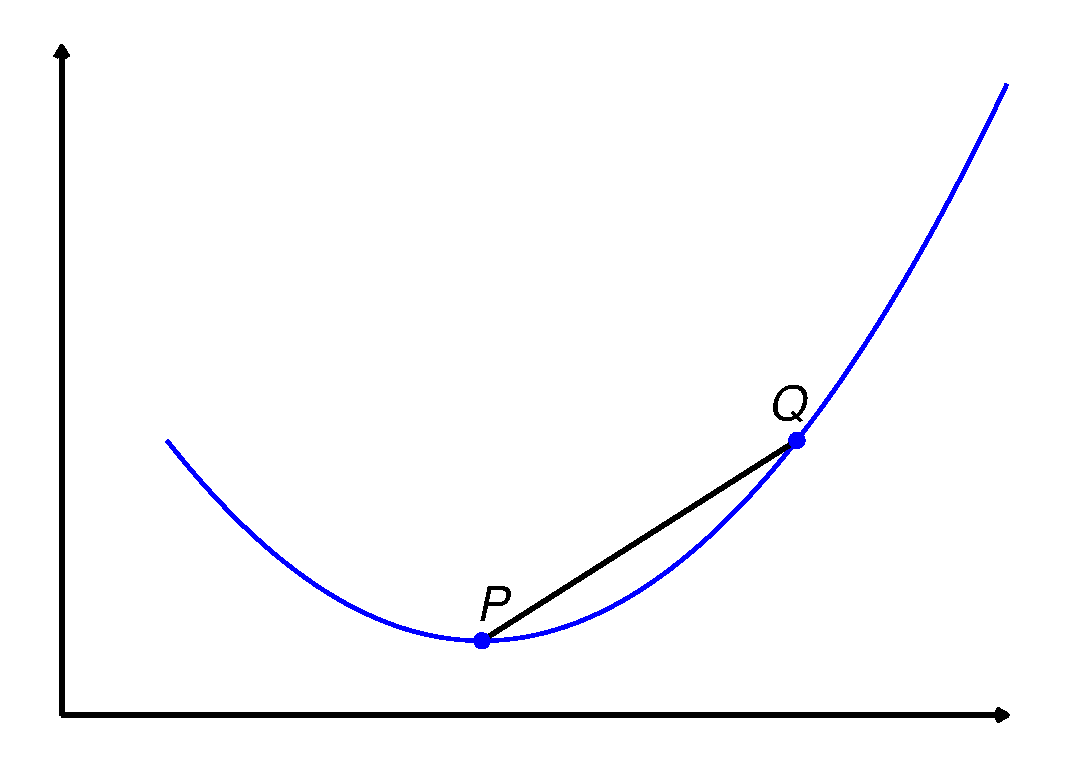
\includegraphics[width=15cm, height=7.9cm]{images/convexo.pdf}}
  \label{fig:convexo}
\end{figure}

\begin{definition}
	Una función $f: D \rightarrow \mathbb{R}$ es concava si $-f$ es convexa
\end{definition}

\begin{theorem}
	Sea $f$ definida en un punto $x_0$. Si $f$ tiene una derivada en $x_0$, entonces es continuo en $x_0$
\end{theorem}
\subsubsection{Demostración}
De la definición de derivada, se determina la siguiente igualdad
\begin{eqnarray}
	\phi(h) &=& \frac{f({x}_{0}+h)-f({x}_{0})}{h} \nonumber \\
	h \phi(h) &=& f({x}_{0}+h)-f({x}_{0}) \nonumber
\end{eqnarray}
Si existe la derivada de $f(x)$ en ${x}_{0}$, entonces $\phi(h) \rightarrow {f}^{'}({x}_{0})$ y como $h \rightarrow 0$ la expresión se desprende como
$$
f({x}_{0}+h) - f({x}_{0}) \rightarrow 0
$$
Por lo que para un determinado $\epsilon > 0$ existe un $\delta > 0$ tal que
$$
\lvert f({x}_{0}+h)-f({x}_{0}) \rvert < \epsilon
$$
Si $\lvert h \rvert < \delta$, se indica que $f(x)$ es continuo en ${x}_{0}$

%\begin{theorem}(\citep{Boyd_2004})
%	\label{convexo_dos_derivadas}
%	\begin{itemize}
%		\item[i] Si asumimos que $f$ es dos veces diferenciable, esto es la matriz Hessiana de segundo orden. Entonces $f$ es convexo si y solo si el dominio de $f$ es convexo y la matriz Hessiana es positiva semidefinida para todo $x \in dom(f)$
%		$$
%				{\nabla}^{2}f(x) \geq 0
%		$$
%		\item[ii] Si asumimos que $f$ es dos veces diferenciable, esto es la matriz Hessiana de segundo orden. Entonces $f$ es cóncavo si y solo si el dominio de $f$ es convexo y la matriz Hessiana es negativa semidefinida para todo $x \in dom(f)$
%		$$
%				{\nabla}^{2}f(x) \leq 0
%		$$
%	\end{itemize}
%\end{theorem}

\subsection{Máximo y mínimo de una función}
Para encontrar los máximos y mínimos de una función que sirve para hallar los valores óptimos, se debe encontrar los extremos de la función $f$ definida por $y=f(x)$ cuya derivada $f'(x)$ existe en cualquier conjunto abierto dentro de su dominio. \citep{Khuri_2002}

\begin{definition}
	Una función $f: D \rightarrow \mathbb{R}$ tiene un maximo local en un punto ${x}_{0} \in D$ si existe $\delta > 0$ tal que $f(x) \leq f({x}_{0})$ para todo $x \in {N}_{\delta}({x}_{0}) \cap D$. La función $f$ tiene un mínimo local en ${x}_{0}$ si $f(x) \geq f({x}_{0})$ para todo $x \in {N}_{\delta}({x}_{0}) \cap D$.
\end{definition}

\begin{definition}
	Una función $f: D \rightarrow \mathbb{R}$ tiene un máximo absoluto encima de $D$ si existe un punto $x^* \in D$ tal que $f(x) \leq f(x^*)$ para todo $x \in D$. La función $f$ tiene un mínimo absoluto encima de $D$ si existe un punto $x^* \in D$ tal que $f(x) \geq f(x^*)$ para todo $x \in D$.
\end{definition}

La determinación de los óptimos locales de $f$ son facilitados si $f$ es diferenciable

\begin{theorem}
	\label{teorema_min_max}
	Sea $f(x)$ diferenciable en un intervalo abierto $(a,b)$. Si $f(x)$ tiene un máximo o mínimo local en un punto ${x}_{0}$ en $(a,b)$, entonces $f'({x}_{0})=0$
\end{theorem}
\subsubsection{Demostración}
Suponga que $f$ tiene un máximo local en ${x}_{0}$. Entonces $f(x) \leq f({x}_{0})$ para todo $x$ en una vecindad ${N}_{\delta}({x}_{0}) \subset (a,b)$ resulta
\begin{equation}
	\frac{f(x)-f({x}_{0})}{x-{x}_{0}} =
	\left\{
	\begin{array}{ll}
		\leq 0, & \text{si } x > {x}_{0} \\
		\geq 0, & \text{si } x < {x}_{0}
	\end{array}
	\right.
\end{equation}
Para todo $x$ que pertenece a ${N}_{\delta}({x}_{0})$ como $x \rightarrow {x}_{0}^{+}$ la relación tendrá un límite no positivo, y si $x \rightarrow {x}_{0}^{-}$ la relación tendrá un límite no negativo. Mientras $f'(x_0)$ exista estos dos límites deben ser iguales a $f'({x}_{0})$ como $x \rightarrow {x}_{0}$ en lo que se concluye que $f'({x}_{0})=0$.

De igual forma suponga que $f(x)$ tiene un mínimo local en ${x}_{0}$. Entonces $f(x) \geq f({x}_{0})$ para todo $x$ en una vecindad ${N}_{\delta}({x}_{0}) \subset (a,b)$ resulta
\begin{equation}
	\frac{f(x)-f({x}_{0})}{x-{x}_{0}} =
	\left\{
	\begin{array}{ll}
		\geq 0, & \text{si } x > {x}_{0} \\
		\leq 0, & \text{si } x < {x}_{0}
	\end{array}
	\right.
\end{equation}
Para todo $x$ que pertenece a ${N}_{\delta}({x}_{0})$ como $x \rightarrow {x}_{0}^{+}$ la relación tendrá un límite no negativo, y si $x \rightarrow {x}_{0}^{-}$ la relación tendrá un límite no positivo. Mientras $f'(x_0)$ exista estos dos límites deben ser iguales a $f'({x}_{0})$ como $x \rightarrow {x}_{0}$ en lo que se concluye que $f'({x}_{0})=0$.

Una aplicación de la segunda derivada es la prueba para identificar valores máximos y mínimos locales como una consecuencia de la prueba de concavidad que sirve como alternativa a la primera prueba de la derivada \citep{stewart2016calculus}

\begin{itemize}
	\item \textbf{Prueba de la segunda derivada} Suponga que $f''$ es continuo cerca de un punto $c$.
	\begin{itemize}
		\item[\textbf{a)}] Si $f'(c)=0$ y $f''(c) > 0$, entonces $f$ tiene un mínimo local en $c$.
		\item[\textbf{b)}] Si $f'(c)=0$ y $f''(c) < 0$, entonces $f$ tiene un máximo local en $c$.
	\end{itemize}
\end{itemize}

\subsection{Variable aleatoria}
El concepto de variable aleatoria se define como una función del espacio muestral en el conjunto de números reales, esto permite considerar el resultado de un experimento aleatorio como un número real tomado por la variable aleatoria \citep{rincon2014introduccion}.

En general la variable aleatoria asigna un número real $x$ a cada elemento $e$ del espacio muestral $\Omega$. El dominio de $X$ es $\Omega$ y los números en el rango son números reales, en el cual la función $X$ se denomina variable aleatoria \citep{hines1988probabilidad}.

\begin{definition}
	Si $E$ es un experimento aleatorio que tiene espacio muestral $\Omega$, y $X$ es una función que asigna un número real $X(e)$ para todo resultado $e \in \Omega$, entonces $X(e)$ se llama variable aleatoria.
\end{definition}

\subsubsection{Función de distribución}
Por convención se utiliza una letra minúscula para denotar un valor particular de una variable aleatoria, del modo que $(X=x)$ es un evento del espacio del rango de la variable aleatoria $X$, donde $x$ es un número real. La probabilidad del evento $(X \leq x)$ puede expresarse como la función de $x$ en la siguiente forma
\begin{equation}
	F(x)=P(X \leq x)
\end{equation}
Donde $F(x)$ es llamada función de distribución, o función de distribución acumulativa de la variable aleatoria $X$

\subsection{Variable aleatoria discreta}\label{VADiscreta}
Generalmente estan relacionados al conteo, en el cual si $X$ es una variable aleatoria discreta, entonces $F(x)$ tendrá un número contablemente infinito de saltos y su rango $R=\{{x}_{1},{x}_{2},\ldots,{x}_{k},\ldots\}$
\begin{definition}\label{defn_vadisc}
	Si $X$ es una variable aleatoria discreta, asociamos un número\\ $p({x}_{i})=P(X={x}_{i})$ con cada resultado ${x}_{i}$, en $R$ para $i=1,2, \ldots , n, \ldots$ donde los números $p({x}_{i})$ satisfacen
	\begin{enumerate}
		\item $p({x}_{i}) \geq 0 \quad$ para todo $i$
		\item $\sum\limits_{i = 1}^{x}p({x}_{i})=1$ 
	\end{enumerate}
\end{definition}
En lo cual se observa que 
\begin{equation}
	\label{eq:prob:p_xi}
	p({x}_{i})=F({x}_{i})-F({x}_{i-1})
\end{equation}
y
\begin{equation}
	\label{eq:prob:p_xi2}
	F({x}_{i})=P(X \leq {x}_{i}) = \sum\limits_{x \leq {x}_{i}}^{}p(x)
\end{equation}
Empleando la ecuación (\ref{eq:prob:p_xi}) notamos el siguiente resultado para $b \geq a$
\begin{equation}
	P(a < X \leq b) = F(b) - F(a)
\end{equation}

\subsubsection{Esperanza}
Sea $X$ una variable aleatoria discreta con función de probabilidad $f(x)$. La esperanza de $X$ se define como el número
\begin{equation}
	E(X)=\sum\limits_{x}^{}xf(x)
\end{equation}

\subsubsection{Varianza}
Sea $X$ una variable aleatoria discreta con función de probabilidad $f(x)$. La varianza de $X$ se define como el número
\begin{equation}
	Var(X)=\sum\limits_{x}^{}{(x-\mu)}^{2}f(x)
\end{equation}
Donde $\mu$ es la esperanza de $X$ ($E[X]$) \citep{rincon2014introduccion}

\subsection{Variable aleatoria continua}\label{VAContinua}
En este caso se tiene un tramo continuo en los cuales el rango $R$ consistirá en uno o más intervalos, en la cual se define la función de densidad $f(x)$ como
\begin{equation}
	f(x) = \frac{d}{dx}F(x)
\end{equation}
y resulta que
\begin{equation}
	F(x) = \int_{- \infty}^{x}f(t)dt
\end{equation}
En la cual tiene la misma forma que (\ref{eq:prob:p_xi2}) reemplazando el simbolo de la sumatoria por la integral, entonces se tienen las siguientes propiedades de $f(x)$
\begin{enumerate}
	\item $f(x)\geq 0 \quad$ para todo $x \in {R}_{x}$
	\item $\int_{{R}_{x}}^{}f(x)dx=1$
	\item $f(x)$ es un tramo continuo.
	\item $F(x)=0$ si $x \notin {R}_{x}$ 
\end{enumerate}
De la misma forma en un rango para $x$ la función $f$ es estable si cumple lo siguiente
\begin{equation}
	P\{ e \in \Omega: a \leq X(e) \leq b \} = \int_{b}^{a}f(x)dx
\end{equation}
\citep{hines1988probabilidad}

\subsubsection{Esperanza}
Sea $X$ una variable aleatoria continua con función de densidad $f(x)$, la esperanza esta definida como
\begin{equation}
	E(X) = \int_{- \infty}^{\infty} xf(x)dx
\end{equation}
Suponiendo que esta integral es absolutamente convergente, es decir, cuando la integral de los valores absolutos es convergente.

\subsubsection{Varianza}
Sea $X$ una variable aleatoria continua con función de densidad $f(x)$. La varianza de $X$ se define como el número
\begin{equation}
	Var(X)= \int_{- \infty}^{\infty} {(x-\mu)}^{2} f(x)dx
\end{equation}
Donde $\mu$ es la esperanza de $X$ ($E[X]$), además de que esta integral debe ser convergente \citep{rincon2014introduccion}.

\subsection{Distribución normal}\label{Dist_normal}
La distribución normal es de las más importantes tanto en la parte teórica como la aplicativa de la estadística \citep{hines1988probabilidad}. Se afirma que una variable aleatoria $X$ tiene una distribución normal con media $\mu (- \infty < \mu < \infty)$ y varianza ${\sigma}^{2} > 0$ y tiene la función de densidad
\begin{equation}
	\label{distribucion_normal}
	f(x) = \frac{1}{\sigma \sqrt{2 \pi}} {e}^{-\frac{1}{2} {\left( \frac{x- \mu}{\sigma} \right)}^{2}}
\end{equation}

Con media $\mu$ y varianza ${\sigma}^{2}$. Su notación abreviada es $X \sim N(\mu, {\sigma}^{2})$ para indicar que la variable aleatoria $X$ se distribuye normalmente con media $\mu$ y varianza ${\sigma}^{2}$.

\subsubsection{Distribución normal acumulativa}
La función de distribución acumulativa $F$ es
\begin{equation}
	F(x) = P(X \leq x) = \int_{-\infty}^{x} \frac{1}{\sigma \sqrt{2 \pi}} {e}^{-\frac{1}{2} {\left( \frac{x- \mu}{\sigma} \right)}^{2}} d \mu
\end{equation}
La evaluación de la integral es muy complicado, por lo que es necesario aplicar métodos numéricos. Sin embargo una transformación de variables $z = \frac{x-\mu}{\sigma}$, permite que la evaluación sea independiente de $\mu$ y $\sigma$. de la siguiente forma
\begin{eqnarray}
	F(x) &=& P(X \leq x) = P \left( Z \leq \frac{x-\mu}{\sigma} \right) \nonumber \\
	F(x) &=& \int_{- \infty}^{(x-\mu) / \sigma} \frac{1}{\sqrt{2 \pi}} {e}^{- \frac{{z}^{2}}{2}}dz \nonumber \\
	\label{distribucion_normal_acum}
	F(x) &=& \int_{- \infty}^{(x - \mu)/ \sigma} \varphi (z)dz \nonumber \\
	F(x) &=& \Phi \left( \frac{x-\mu}{\sigma} \right)
\end{eqnarray}

\subsubsection{Distribución normal estándar}
De la distribución de probabilidad en (\ref{distribucion_normal_acum}) se tiene
\begin{equation}
	\varphi (z) = \frac{1}{\sqrt{2 \pi}} {e}^{- \frac{{z}^{2}}{2}} \quad -\infty < z < \infty
\end{equation}
Es una distribución normal con media $0$ y varianza $1$, esto indica que $Z \sim N(0,1)$ en la cual $Z$ es una \textsl{distribución normal estándar}, su gráfica de función de densidad se muestra en la Figura \ref{fig:norm_z}.
\begin{figure}[H]
  \caption{Distribución normal estándar $Z \sim N(0,1)$}
  {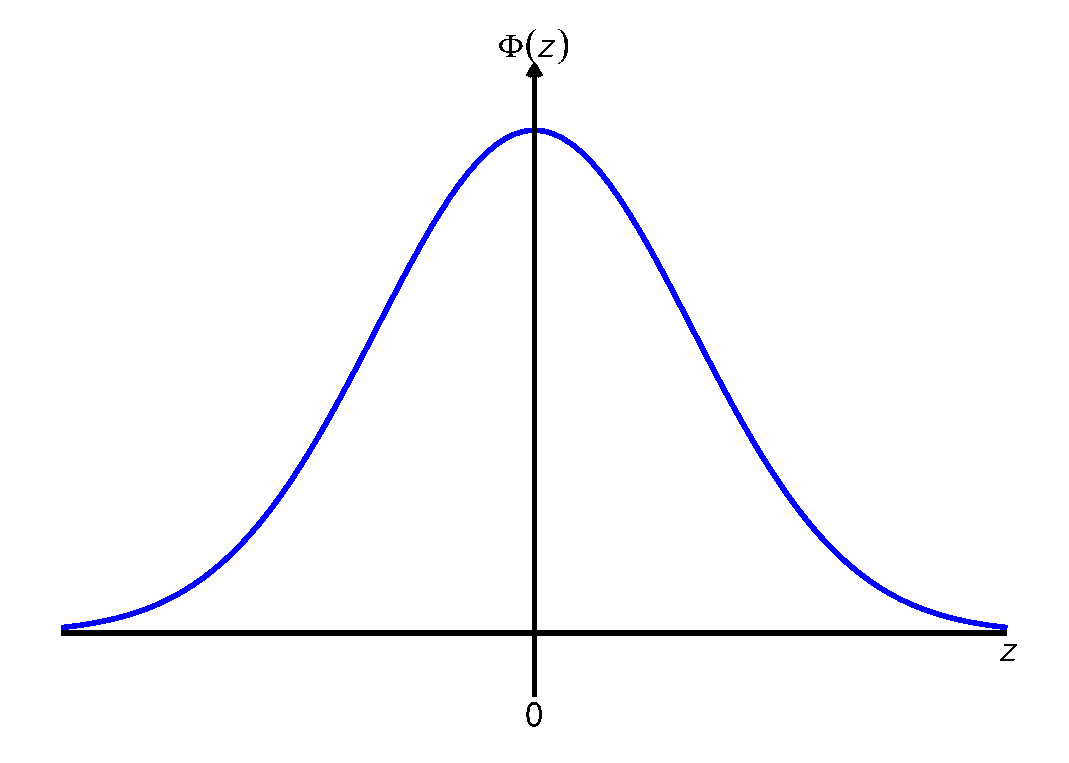
\includegraphics[width=15cm, height=7.9cm]{images/norm_estn.pdf}}
  \label{fig:norm_z}
\end{figure}

La función de distribución correspondiente ahora es $\Phi$
\begin{equation}
	\Phi (z) = \int_{-\infty}^{z} \frac{1}{\sqrt{2 \pi}} {e}^{- \frac{{z}^{2}}{2}} dz
\end{equation}

\subsection{Costos}
La contabilidad de costos determina el costo estimado hacia el real del producto o servicio para valorarlo y considerarlo en su precio de venta. La gestión de costos es la actividad de medición y análisis. \citep{toomey2000inventory}

Los costos deben considerar tanto los costos directos e indirectos, como por ejemplo el costo directo viene a ser el costo de compra mientras que los costos indirectos viene a ser los gastos generales de fabricación y materiales. \cite{haeussler2003matematicas} indican que el \textsl{costo fijo} es la suma de costos independientes del nivel de producción como renta, seguros entre otros; mientras que el \textsl{costo variable} es la suma de todos los costos dependientes del nivel de producción como salarios y materiales. De esta forma el \textsl{costo total} es la suma de los costos variables y fijos.

\newpage
\subsection{Clasificación de actividades basada en costos (ABC)}
\label{section:ABC}
\cite{toomey2000inventory} lo indica como un modo alternativo a la gestión de costos en el cual se acumulan los costos de los productos o servicios brindados de tal forma que clasifica los trabajos en base a sus costos acumulados, en lugar de categorías contables que permita una gestión de costos efectiva. Su propósito es dividir todos los productos o articulos que se tienen en el inventario y clasificarlas en tres grupos (A, B y C), en el cual se le debe dedicar más tiempo a la administración a los productos que representan el mayor costo monetario \citep{render2006metodos}.

La clasificación de los productos son descritos a continuación:
\begin{enumerate}
	\item \textbf{Grupo A:} Son los productos que poseen la mayor parte de los costos de todo el inventario que suele conformar el $70\%$, sus niveles de inventario deben ser monitoreados con una prioridad alta aunque estos solo comprendan el $10\%$ de todos los artículos del inventario, siendo así su tiempo de dedicación no muy alto.
	\item \textbf{Grupo B:} Son los productos que poseen costos moderados de todo el inventario conformando el $20\%$ siendo menores a los del grupo A, sus productos comprenden también el $20\%$ de todos los artículos del inventario, por lo cual su tiempo de dedicación debería ser menor a los del grupo A, especialmente a los costos más altos del grupo B.
	\item \textbf{Grupo C:} Son los productos que poseen la menor cantidad de costos del inventario conformando solo el $10\%$, aunque sus productos comprenden el $70\%$ de todo el inventario. Para este grupo no es beneficioso dedicar mucho tiempo a la administración de sus artículos como a los de grupo A y B.
\end{enumerate} 
La Tabla \ref{table:ABC_resumen} resume el análisis ABC.
\begin{table}[h!]
    \caption{Resumen de actividades basadas en costos (ABC)}
    \begin{tabular}{p{0.8cm} p{2.52cm} p{5.2cm} p{4.9cm}} % Define anchos personalizados para cada columna
        \hline
        \textbf{Grupo} & \textbf{$(\%)$ de Costos} & \textbf{$(\%)$ ocupación del inventario} & \textbf{Usar técnicas cuantitativas} \\
        \hline
        \textbf{A} & $70\%$ & $10\%$ & Si \\
        \textbf{B} & $20\%$ & $20\%$ & Los que tienen costos altos \\
        \textbf{C} & $10\%$ & $70\%$ & No \\
        \hline
    \end{tabular}
    \label{table:ABC_resumen}
\end{table}


\subsection{Inventarios}
La sociedad estadounidense de producción e inventario (APICS) lo define como la rama de la gestión empresarial que se ocupa de la planificación y el control de inventarios, en el cual su función es mantener un nivel de existencias deseado de productos o artículos específicos. \citep{toomey2000inventory}

El rol principal del inventario es servir o brindar servicio al cliente, esto implica factores como la disponibilidad de la cantidad pedida, momento correcto, lugar correcto y costo correcto. Su objetivo principal es minimizar las inversiones en inventarios y al mismo tiempo cumplir con los requisitos funcionales sin alterar las operaciones normales.

Un sistema que controla los inventarios tiene que ser compatible con los objetivos, funciones y demandas del inventario en particular.

\subsection{Modelos de inventarios}

%\subsection{Modelo General de Inventario}

Los problemas de inventarios son relacionados sobre reservas de cierto artículo o insumo utilizado para satisfacer las demandas. Por lo cual el exceso de existencias provoca un mayor costo de capital y almacenamiento, mientras que el desabesticimiento interrumpe las producciones y/o las ventas. En el que se debe optimizar el nivel de inventario que equilibre las dos situaciones minimizando una función de costo apropiada. Esto se define en diseñar una \textsl{política de inventario} \citep{taha2012investigacion} que responda las preguntas:

\begin{enumerate}
	\item ¿Cuánto pedir?
	\item ¿Cuándo pedir?
\end{enumerate}

En la cual su base del modelo de inventario es la siguiente función de costo genérica para el costo total del inventario $CTI(y)$

$$
\begin{pmatrix}
\text{Costo total del} \\ 
\text{inventario}
\end{pmatrix}
=
\begin{pmatrix}
\text{Costo de} \\ 
\text{compra}
\end{pmatrix}
+
\begin{pmatrix}
\text{Costo de} \\ 
\text{preparación}
\end{pmatrix}
+
\begin{pmatrix}
\text{Costo de} \\ 
\text{retención}
\end{pmatrix}
+
\begin{pmatrix}
\text{Costo por} \\ 
\text{escasez}
\end{pmatrix}
$$

Donde:

\begin{enumerate}
	\item \textbf{Costo de compra $(C)$: }Es el costo por unidad de un artículo de inventario. Puede haber momentos en que el artículo se ofrece con descuento si el tamaño del pedido excede una cantidad determinada, lo cual es un factor importante a tomar en cuenta al momento de tomar la decisión de \textsl{cuánto pedir}.

	\item \textbf{Costo de preparación $(K)$: }Representa los costos que incurren cuando se coloca un pedido, es decir los costos que llevan la elaboración o brindación del servicio o su producto independientemente de su tamaño.

	\item \textbf{Costo de retención (almacenamiento) $(h)$: }Representa el costo de mantener las existencias de productos sobrantes. Estos costos incluyen el interés sobre el capital y el costo de almacenamiento, mantenimiento y manejo del producto.

	\item \textbf{Costo por escasez (faltante) $(p)$: }Este costo es tomado como una penalización en que se incurre cuando se agotan las existencias. Incluye la pérdida potencial de ingresos, la interrupción de la producción y el costo subjetivo de pérdida de lealtad del cliente debido a la falta del producto.
\end{enumerate}

Esto también puede expresarse de la siguiente manera:
\begin{equation}
	\label{2.1}
	CTI(y) = C + K + h + p
\end{equation}

\subsection{Política sobre un modelo de inventarios}

Entonces se hacen las siguientes preguntas sobre cuando y cuanto debe reabastecerse un inventario. Por el cual la administración científica de inventarios debe comprender los siguientes pasos:
\begin{enumerate}
	\item Plantear un \textsl{modelo matemático} que describa el comportamiento del sistema de inventarios.
	\item Elaborar una política óptima de inventarios a partir del modelo.
	\item Utilizar un \textsl{sistema de procesamiento de información computarizado} para mantener registros de los niveles del inventario.
	\item A partir de estos registros, utilizar la política óptima de inventarios para señalar cuándo y cuánto conviene reabastecer. 
\end{enumerate}

Los modelos matemáticos de inventarios que se utilizan bajo estos pasos son los modelos determinísticos y estocásticos, el modelo dependerá según la posibilidad de predecir la demanda. \citep{hillier2003introduccion}

\subsection{Clasificación de un sistema de inventarios}

Asimismo un sistema de inventario puede requerir \textsl{revisiones periódicas} es decir en un cierto intervalo de tiempo como una semana o cada mes. De forma alterna puede estar basado en \textsl{revisiones continuas}, que es cuando se realiza un pedido cuando el nivel del inventario se reduce a un punto de volver a pedir o \textsl{punto de reorden (R)}.

\subsection{Demanda}
La complejidad de los modelos de inventario depende de si la demanda ($D$) es determinística o probabilística, además que esta pueda variar con el tiempo. \citep{hillier2003introduccion}

Cuando se tiene una demanda determinística se conocen los pedidos siguientes, asimismo sobre intervalos de tiempos iguales la demanda puede ser constante (estática) o variable (dinámica).

En el caso de una demanda probabilística se efectúa cuando la demanda en un periodo de tiempo es incierta, pero puede describirse en términos de una distribución de probabilidad, en el caso de las demandas probabilísticas se tienen que estas puedan ser estacionarias o no estacionarias sobre el tiempo.

%De forma general el patrón de la demanda en un modelo de inventario puede asumir uno de estos tipos:
%\begin{enumerate}
%	\item Determinístico y constante (estático) con el tiempo.
%	\item Determinístico y variable (dinámico) con el tiempo.
%	\item Probabilístico y estacionario a lo largo del tiempo.
%	\item Probabilístico y no estacionario a lo largo del tiempo. 
%\end{enumerate}

Entonces para seleccionar el modelo de inventario, debemos determinar si se va a utilizar un modelo determinístico o probabilístico. Esta decisión es más factible calculando el \textsl{coeficiente de variabilidad} $(CV)$ tomando los siguientes pasos
\begin{enumerate}
	\item Calcular la demanda promedio en el periodo evaluado es decir tomar la \textsl{Media}.
	$$
	\textsl{Media}=\frac{1}{n}\sum\limits_{i = 1}^{n}{d}_{i}
	$$
	\item Encontrar una estimación de la varianza de la demanda por periodo, es decir tomar la \textsl{Varianza}.
	$$
	\textsl{Varianza}=\frac{1}{n}\sum\limits_{i = 1}^{n}{(d_i-\textsl{Media})}^2
	$$
	\item Determinar el coeficiente de variabilidad ($CV$) que representa la variabilidad relativa de la demanda con la siguiente fórmula
	\begin{equation}
	\label{CVar}
	CV = \frac{\textsl{Varianza}}{\textsl{Media}^2}
\end{equation}
	\item Si el ($CV$) (\ref{CVar}) es menor a 0.20, indica que la demanda es relativamente estable en los periodos evaluados, y por lo tanto tiene una demanda determinística. Si resulta mayor o igual a 0.20 indica que la demanda no es estable y además, por lo que posee una demanda probabilística.
\end{enumerate}


%\subsection{Multiplicadores de Lagrange}
%Un importante teorema que ayuda en funciones restringidas es el de ``Multiplicadores de Lagrange'' formulada por Joseph-Louis Lagrange, más conocido como Giuseppe Luigi Lagrangia, quien fue un físico, matemático y astrónomo italiano nacido en Turín el 25 de enero de 1736. Además de sus principales logros fue demostrar el teorema del valor medio, desarrollar la mecánica Lagrangiana y su importante contribución en astronomía. Falleciendo en Paris el 10 de abril de 1813. \citep{cardenascalculo}

\subsection{Modelos de inventario determinísticos}

Este modelo asume que la demanda y el tiempo de entrega son conocidos y fijos, adicionalmente en los modelos estáticos se tiene una demanda constante en función del tiempo. \citep{taha2012investigacion}

\manualsubsubsection{2.2.15.1}{Modelo clásico de cantidad económica de pedido (EOQ)}\label{Modelo_clas_EOQ}
La abreviación EOQ proviene del inglés (economic order quantity) que significa cantidad económica pedido. Este primer modelo asume que la demanda es constante y las ordenes llegan en el momento que se están solicitando. Se basa en los siguientes supuestos:
\begin{enumerate}
	\item Tasa de demanda conocida por unidad de tiempo.
	\item La cantidad ordenada de inventario llega cuando se desea, indicando un tiempo de espera igual a cero.
	\item No se tienen faltantes.
\end{enumerate}
\clearpage
Como la demanda es constante a través de los intervalos de tiempo, se tiene un inventario disminuido con comportamiento uniforme, de tal forma que cuando el inventario llega a una cantidad nula o cero, con el nuevo pedido este nivel de inventario debe incrementarse a ``$y$'' unidades. El proceso continuará con esta conducta a través del tiempo.

Según al modelo se definen las siguientes componentes:

\begin{itemize}
	\item[$y=$] Cantidad de pedido, que viene a ser el número de unidades pedidas.
	\item[$D=$] Tasa de demanda, expresado en las unidades de medidas sobre el tiempo evaluado.
	\item[$T=$] Duración del ciclo de pedido, expresado en el tiempo evaluado desde el momento que se tiene el pedido hasta el siguiente pedido.
\end{itemize}

Gráficamente se puede observar en la Figura \ref{fig:img1} la conducta del modelo clásico de cantidad económica de pedido.

\begin{figure}[H] %Colocar H mayuscula en lugar del h!
  \caption{Conducta de inventario en el modelo clásico económica de pedido (EOQ)}
  {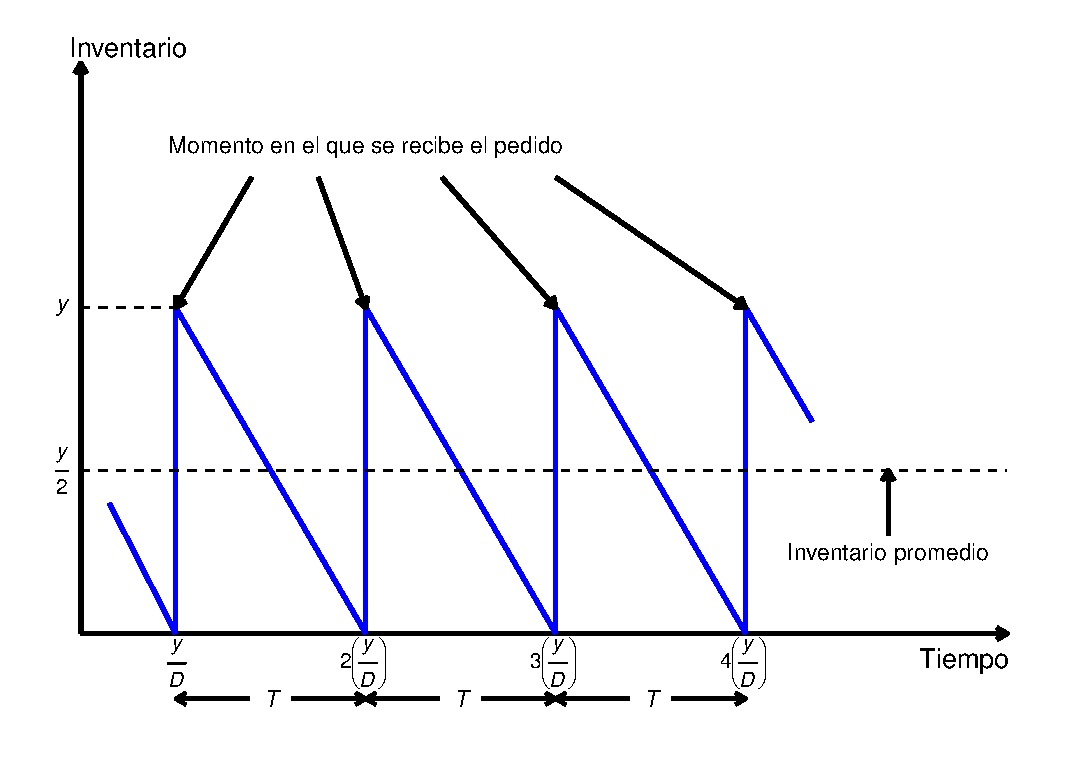
\includegraphics[width=15cm, height=8.5cm]{images/img1.pdf}}
  \label{fig:img1}
\end{figure}

Durante los pedidos, se tiene un intervalo de tiempo que comienza con el abastecimiento del pedido y culmina en el punto en el que se recibe el siguiente abastecimiento del pedido, por tanto se tiene la siguiente relación
\begin{equation}
	\label{T}
	T = \frac{y}{D}
\end{equation}

Para el modelo de costos del modelo EOQ se requieren dos parámetros esenciales
\begin{itemize}
	\item[$K=$] Costo de preparación del pedido
	\item[$h=$] Costo de retención
\end{itemize}

El nivel de inventario promedio ($NIP$) que se mide en unidades sobre el tiempo se encuentra expresado de la siguiente forma:
\begin{equation}
	\label{NIP}
	NIP=\frac{y}{2}
\end{equation}

El costo de almacenamiento por unidad de tiempo ($CAT$) estaría en función del costo de almacenamiento $h$ por el nivel promedio de inventario $(NIP)$ expresado en la ecuación (\ref{NIP}):
\begin{eqnarray}
	\label{CAT}
	CAT &=& h(NIP) \nonumber \\
	CAT &=& h\left(\frac{y}{2} \right)
\end{eqnarray}
Entonces el costo de almacenamiento por intervalo de tiempo ($CAIT$) vendría a estar expresado como el producto del tiempo entre abastecimientos del producto por el costo de almacenamiento por unidad de tiempo, de la siguiente forma:
\begin{eqnarray}
	CAIT = T * CAT \nonumber
\end{eqnarray}
Reemplazando los valores por las expresiones (\ref{T}) y (\ref{CAT}) se tiene la siguiente expresión para el costo de almacenamiento por intervalo de tiempo 
\begin{eqnarray}
	\label{CAIT}
	CAIT &=&  \left( \frac{y}{D} \right)  \left[ h \left( \frac{y}{2} \right) \right]  \nonumber \\
	CAIT &=& \frac{h {y}^{2}}{2D}
\end{eqnarray}
Ahora el costo por cada orden realizada o costo por la producción en el intervalo de tiempo ($CPT$) estaría expresado como:
\begin{equation}
	\label{CPT}
	CPT = K + Cy
\end{equation}
De lo que el costo total por intervalo de tiempo ($CTT$) sería el costo de almacenamiento por intervalo de tiempo (\ref{CAIT}) más el costo de producción por intervalo de tiempo (\ref{CPT})
\begin{eqnarray}
	\label{CTT}
	CTT &=& CAIT + CPT \nonumber \\
	CTT &=& \frac{h {y}^{2}}{2D} + K + Cy
\end{eqnarray}
Si al costo total por intervalo de tiempo ($CTT$) de la expresión (\ref{CTT}) lo dividimos entre el tiempo $T$, se tendría el costo total del inventario ($CTI$)
\begin{eqnarray}
	\label{CTIdejado}
	CTI(y) = \frac{CTT}{T} 
\end{eqnarray}
Reemplazando por los valores de la ecuación (\ref{CTT}) y (\ref{T}) se tiene la siguiente expresión para el costo total del inventario del modelo EOQ
\begin{eqnarray}
	\label{CTI}
	CTI(y) &=& \frac{\frac{h {y}^{2}}{2D} + K + Cy}{\frac{y}{D}} \nonumber \\
	CTI(y) &=& \frac{KD}{y} + DC + \frac{hy}{2}
\end{eqnarray}
De donde se tiene las siguientes componentes
\begin{itemize}
	\item[$\frac{KD}{y}$:] Costo de preparación de pedidos expresado como el costo por pedido multiplicado por el número de pedidos.
	\item[$DC$:] Costo de aprovisionamiento sirve para satisfacer toda la demanda, ya que no se permiten faltantes. Esta en función del producto entre los costos por unidad y la demanda.
	\item[$\frac{hy}{2}$:] Costo de almacenamiento por unidad de tiempo ($CAT$) expresado en (\ref{CAT}).
\end{itemize}	
Se debe minimizar el costo total de inventario $CTI(y)$, en la ecuación (\ref{CTI}) se observa que el $CTI(y)$ esta en función del costo por ordenar y el costo por almacenar.
En todo caso se tiene que minimizar la suma del costo por ordenar y el costo por almacenar, de tal forma que se minimice el costo total de inventario. El valor óptimo de cuanto pedir ``$y$'' es minimizando el $CTI(y)$ mediante la derivación e igualando a cero teniendo como se demostró en el Teorema $\ref{teorema_min_max}$:
\clearpage
\begin{eqnarray}
	\label{dCTI}
	\frac{dCTI(y)}{dy} &=& 0 \nonumber \\
	\frac{dCTI(y)}{dy} &=& \frac{d}{dy}\left(\frac{KD}{y} + DC + \frac{hy}{2} \right) = 0 \nonumber \\
	\frac{dCTI(y)}{dy} &=& - \frac{KD}{y^2} + \frac{h}{2} = 0
\end{eqnarray}
Despejando ``$y$'' en la ecuación (\ref{dCTI}) se obtiene la cantidad de pedido óptima $y^*$ de la siguiente manera
\begin{eqnarray}
	\label{yopt}
	\frac{h}{2} &=& \frac{KD}{y^2} \nonumber \\
	y^2 &=& \frac{2KD}{h} \nonumber \\
	y &=& \pm \sqrt{\frac{2KD}{h}} \qquad \text{(solo se considera la parte positiva)} \nonumber \\
	y^* &=& \sqrt{\frac{2KD}{h}}
\end{eqnarray}
Asimismo la cantidad de pedido es mínima mediante la prueba de la segunda derivada.
\begin{eqnarray}
	\label{minimo1}
	\frac{d^2 CTI(y)}{dy^2} &=& \frac{d^2}{dy^2} \left(\frac{KD}{y} + DC + \frac{hy}{2} \right) \nonumber \\
	\frac{d^2 CTI(y)}{dy^2} &=& \frac{2KD}{y^3} \geq 0; \quad \forall y > 0
\end{eqnarray}
Ahora tomando la ecuación del ciclo de pedido $T$ (\ref{T}) y la cantidad de pedido óptima $y^*$  (\ref{yopt}) se tiene la respuesta a cuando pedir o el intervalo de pedido óptimo $T^*$
%\newpage
\begin{eqnarray}
	\label{Topt}
	T &=& \frac{y}{D} \nonumber \\
	T^* &=& \frac{y^*}{D} \nonumber \\
	T^* &=& \frac{\sqrt{\frac{2KD}{h}}}{D} \nonumber \\
	T^* &=& \sqrt{\frac{2K}{Dh}}
\end{eqnarray}
De la misma forma tomando la ecuación de costo total de inventario $CTI(y)$ (\ref{CTI}) reemplazando con los valores de la cantidad de pedido óptima $y^*$ (\ref{yopt}) se obtiene el costo mínimo total de inventario óptimo $CTI(y^*)$
\begin{eqnarray}
	\label{CTIopt}
	CTI(y) &=& \frac{KD}{y} + DC + \frac{hy}{2} \nonumber \\
	CTI(y^*) &=& \frac{KD}{y^*} + DC + \frac{hy^*}{2} \nonumber \\
%\end{eqnarray}
%Ahora reemplanzando $y^*$ por los valores de (\ref{yopt} se tiene
%\begin{eqnarray}
	CTI(y^*) &=& \frac{KD}{\sqrt{\frac{2KD}{h}}} + DC + \frac{h \left( \sqrt{\frac{2KD}{h}} \right)}{2} \nonumber \\ 
	CTI(y^*) &=& KD \sqrt{\frac{h}{2KD}} + DC + \sqrt{\frac{hKD}{2}} \nonumber \\
	CTI(y^*) &=& \sqrt{\frac{hKD}{2}} + DC + \sqrt{\frac{hKD}{2}} \nonumber \\
	CTI(y^*) &=& 2 \sqrt{\frac{hKD}{2}} + DC \nonumber \\
	CTI(y^*) &=& \sqrt{2hKD} + DC
\end{eqnarray}
Generalmente los pedidos no llegan en el mismo momento que se hace la solicitud de pedido, lo que sucede es un tiempo de espera o tiempo de entrega, que depende a la frecuencia del tiempo ya sean días o hasta semanas. Por lo cual el inventario de igual forma tiene que estar disponible para la demanda una vez ya realizada el pedido. Entonces la decisión de cuándo ordenar es conocida como punto de reorden ($R$) esto se observa en la Figura \ref{fig:img2}.
\begin{figure}[H]
  \caption{Punto de reorden ($R$) del modelo (EOQ)}
  {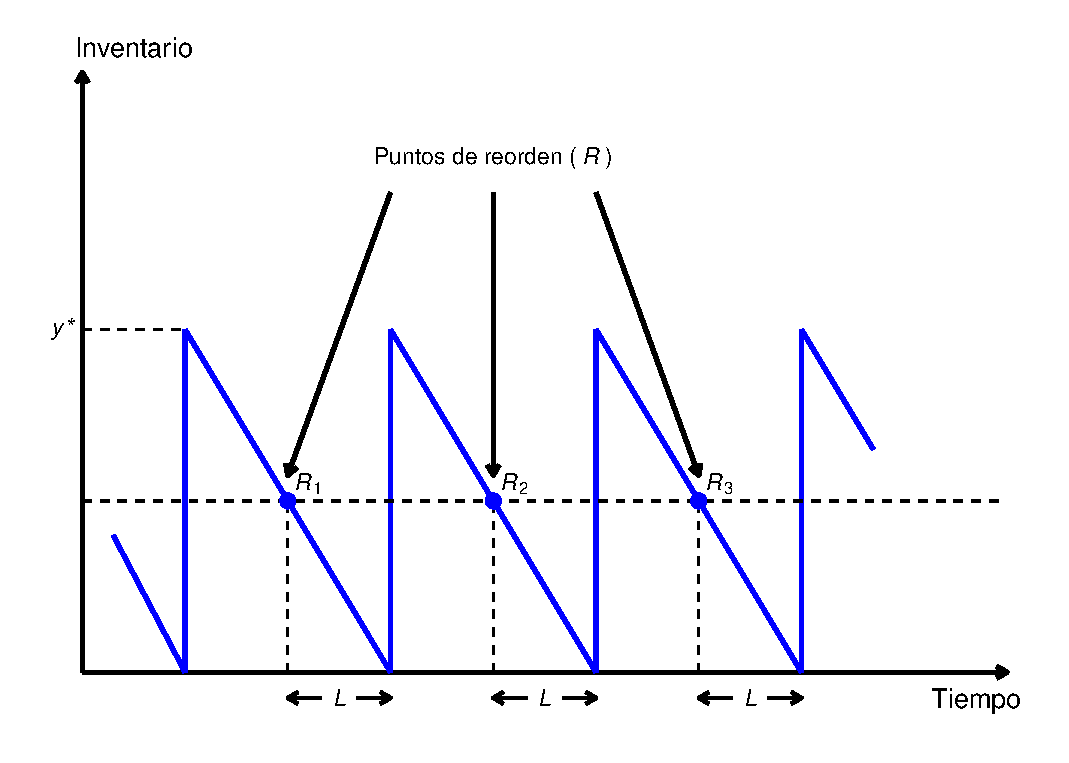
\includegraphics[width=15cm, height=6.5cm]{images/img2.pdf}}
  \label{fig:img2}
\end{figure}

Donde se observa que el punto de reorden se establece tomando en cuenta los siguientes casos. Sea $L$ el tiempo de entrega, entonces el punto de reorden $R$ es:
\begin{itemize}
	\item $R = LD$, si $L < T^*$ es decir que la demanda durante el tiempo de entrega es menor a la cantidad óptima $y^*$, en el cual el punto de reorden es la demanda por el tiempo de entrega.
	\item $L_e = L - nT^*$, si $L > T^*$ es decir que la demanda durante el tiempo de entrega es mayor que la cantidad óptima $y^*$, en el cual el pedido debe realizarse en el periodo del pedido anterior. Por lo que el punto de reorden vuelve a ser
\end{itemize}
$$
	R = L_e D
$$
Por lo cual enunciamos lo siguiente: \textsl{``Pedir la cantidad $y^*$ siempre que el nivel de inventario se reduzca $L_e D$ unidades''}.

\manualsubsubsection{2.2.15.2}{Modelo clásico de cantidad económica de pedido (EOQ) con descuentos}
Algo más general del modelo EOQ es que el precio del producto del inventario  varíe con la cantidad que se compre o produzca. Es decir que se puede obtener un descuento si el tamaño del pedido ``$y$'' excede un límite ``$q$'' establecido. Por lo cual se tiene un precio unitario de compra ``$c$'', expresado de la siguiente manera:
\begin{equation}
	\label{c_descuento}
	c =
	\left\{
	\begin{array}{ll}
		c_1, & \text{si } y \leq q \\
		c_2, & \text{si } y > q
	\end{array}
	\right\}, \quad c_1 > c_2
\end{equation}
De tal forma que el costo de compra por intervalo de tiempo ($CCIT$) estaría en función del precio unitario de compra ``$c$'' (\ref{c_descuento}) y el tiempo de pedido ``$T$'' (\ref{T}), quedando de la siguiente manera
\begin{equation}
	CCIT = \left\{%
	\begin{array}{ll}
		\frac{c_1 y}{T} = \frac{c_1 y}{\left( \frac{y}{D} \right)} = Dc_1 , & y \leq q \\ 
		\frac{c_2 y}{T} = \frac{c_2 y}{\left( \frac{y}{D} \right)} = Dc_2 , & y > q 
	\end{array}%
	\right.
\end{equation}
\clearpage
\noindent Asi mismo si aplicamos la notación utilizada con el precio de compra ``$c$'' (\ref{c_descuento}) en (\ref{CTI}), el costo total de inventario $CTI(y)$ estaría expresado de la siguiente manera
\begin{equation}
	\label{CTI_descuento}
	CTI(y) = \left\{%
	\begin{array}{ll}
		CTI_1 (y) = Dc_1 + \frac{KD}{y} + \frac{hy}{2} , & y \leq q \\ 
		CTI_2 (y) = Dc_2 + \frac{KD}{y} + \frac{hy}{2} , & y > q 
	\end{array}%
	\right.
\end{equation}
En la ecuación (\ref{CTI_descuento}) se observa que $c_i,$ donde $i = \{ 1,2 \}$ actúa como constante si es que deseamos minimizar ``$y$'', e igualar a cero obteniedo nuestra cantidad de pedido óptima $y^*$ tal como se realizó en la expresión (\ref{yopt}) y el Teorema (\ref{teorema_min_max}). Entonces la cantidad óptima de pedido con descuentos $y_m$ es igual a
\begin{equation}
	y_m = \sqrt{\frac{2KD}{h}}
\end{equation}
El costo se ve ilustrado en la Figura \ref{fig:img3}.

\begin{figure}[H]
  \caption{Función de costos de inventario con descuentos en el precio}
  {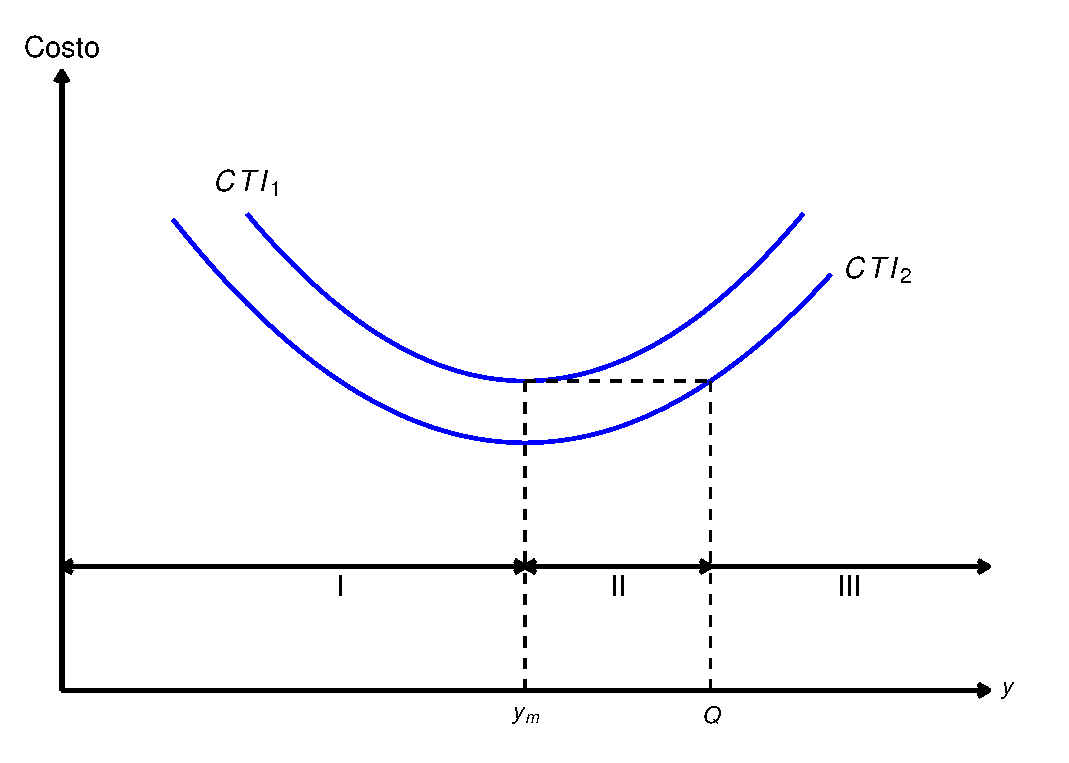
\includegraphics[width=15cm, height=8cm]{images/img3.pdf}}
  \label{fig:img3}
\end{figure} 
En donde la determinación de la cantidad de pedido óptima $y^*$ sera de acuerdo al punto de discontinuidad de precio $q$, con respecto a las zonas I, II y III, limitadas por los intervalos:

\begin{itemize}
	\item \textbf{ZONA I:} en el intervalo $(0, y_m)$
	\item \textbf{ZONA II:} en el intervalo $(y_m, Q)$
	\item \textbf{ZONA III:} en el intervalo $(Q, \infty)$
\end{itemize}

El valor de $Q (> y_m)$ se determina mediante la siguiente ecuación
$$
CTI_2 (Q) = CTI_1 (Q)
$$
Reemplazando $CTI_2 (Q)$ por los valores de la expresión (\ref{CTI_descuento}) se tiene
\begin{eqnarray}
	Dc_2 + \frac{KD}{Q} + \frac{hQ}{2} &=& CTI_1 (Q) \nonumber \\
	\frac{2QDc_2 + 2KD + hQ^2}{2Q} &=& CTI_1 (y_m) \nonumber \\
	2QDc_2 + 2KD + hQ^2 - 2Q [ CTI_1 (ym) ] &=& 0 \nonumber
\end{eqnarray}
A la expresión lo dividimos por el costo de almacenamiento $h \neq 0$ el cual se simplifica en
\begin{eqnarray}
	\label{Q_descuento}
	\frac{2QDc_2 + 2KD + hQ^2 - 2Q [ CTI_1 (ym) ]}{h} &=& \frac{0}{h} \nonumber \\
	\frac{2QDc_2}{h} + \frac{2KD}{h} + \frac{hQ^2}{h} - \frac{2Q [ CTI_1 (y_m) ]}{h} &=& 0 \nonumber \\
	Q^2 + \frac{2QDc_2}{h} - \frac{2Q [ CTI_1 (y_m) ]}{h} + \frac{2KD}{h} &=& 0 \nonumber \\
	Q^2 + \left( \frac{2[ Dc_2 - CTI_1 (y_m) ]}{h} \right) Q + \frac{2KD}{h} &=& 0 
\end{eqnarray}
En la Figura \ref{fig:img4} se muestra la cantidad óptima deseada $y^*$ en base a la zona que se encuentre $q$.
En el cual se observa que la cantidad óptima $y^*$ que se busca es
\begin{equation}
	\label{CTI_descuento2}
	y^* = \left\{%
	\begin{array}{ll}
		y_m & \text{, si } q \text{ se encuentra en las zonas I o III} \\ 
		q & \text{, si } q \text{ se encuentra en la zona II}
	\end{array}%
	\right.
\end{equation}
Los pasos para determinar $y^*$ es
\begin{itemize}
	\item[\textbf{Paso 1:}] Calcular $y_m = \sqrt{\frac{2KD}{h}}$. Si $q$ se encuentra en la zona I, entonces $y^* = y_m$. Caso contrario ir al paso 2.
	\item[\textbf{Paso 2:}] Calcular $Q (> y_m)$. a partir de la ecuación (\ref{Q_descuento}) de $Q$
\end{itemize}
$$
	Q^2 + \left( \frac{2[ Dc_2 - CTI_1 (y_m) ]}{h} \right) Q + \frac{2KD}{h} = 0 
$$
Definir las zonas II y III, si $q$ está en la zona II entonces $y^* = q$. En el caso contrario si $q$ está en la zona III entonces $y^* = y_m$

\begin{figure}[h!]
		\caption{Solución óptima del problema de inventario con descuentos}
    \centering
    % Primera fila con dos imágenes
    \begin{subfigure}[b]{1\textwidth} % Ancho mayor para que sean más grandes
    		\caption{\textbf{Caso 1:} ($q$) queda dentro de la zona I, $y^* = y_m$}
        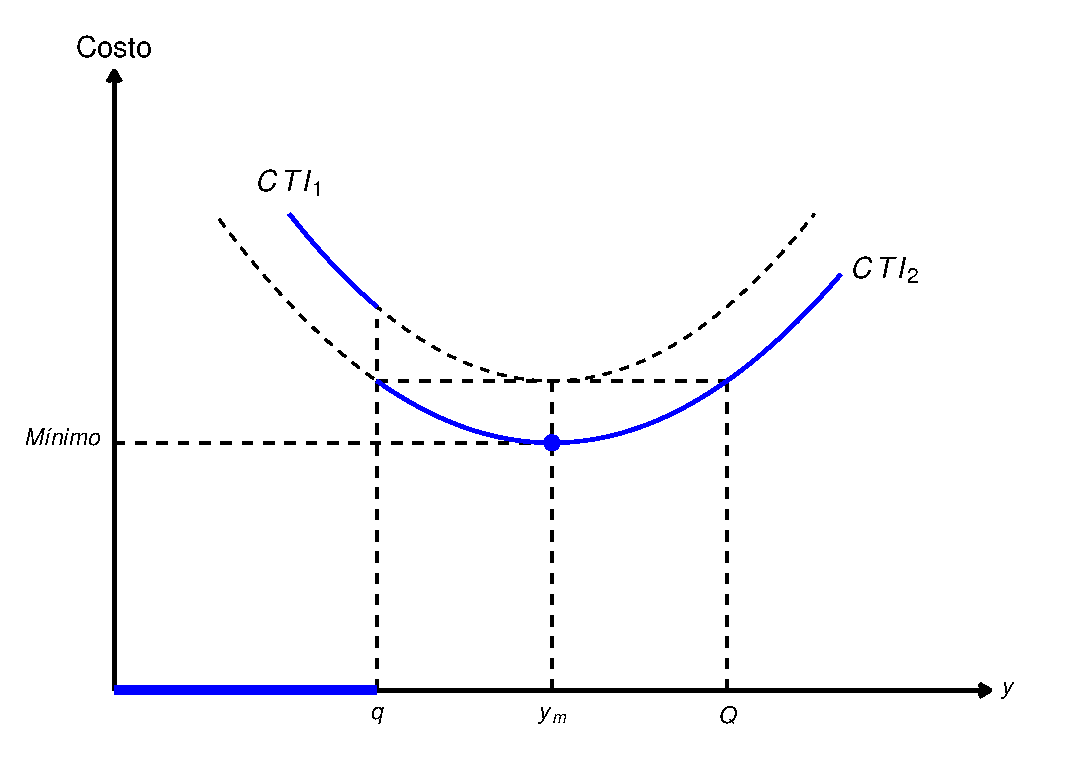
\includegraphics[width=13cm, height=6.1cm]{images/img4.pdf}
        \label{fig:img4a}
    \end{subfigure}

    \vspace{0.2cm}

    \begin{subfigure}[b]{1\textwidth}
    		\caption{\textbf{Caso 2:} ($q$) queda dentro de la zona II, $y^* = q$}
        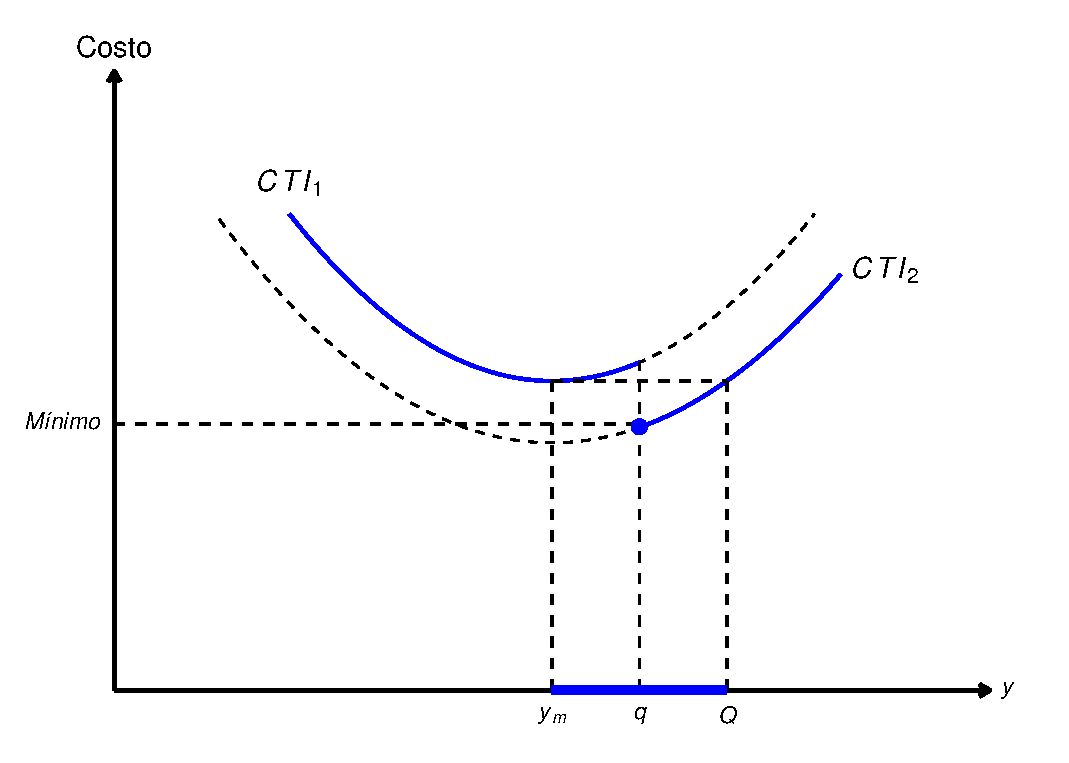
\includegraphics[width=13cm, height=6.1cm]{images/img5.pdf}
        \label{fig:img4b}
    \end{subfigure}
    
    % Salto de línea
    \vspace{0.2cm}
    
    % Segunda fila con una imagen centrada
    \begin{subfigure}[b]{1\textwidth} % Ancho mayor para la tercera imagen
        \caption{\textbf{Caso 3:} ($q$) queda dentro de la zona III, $y^* = y_m$}
        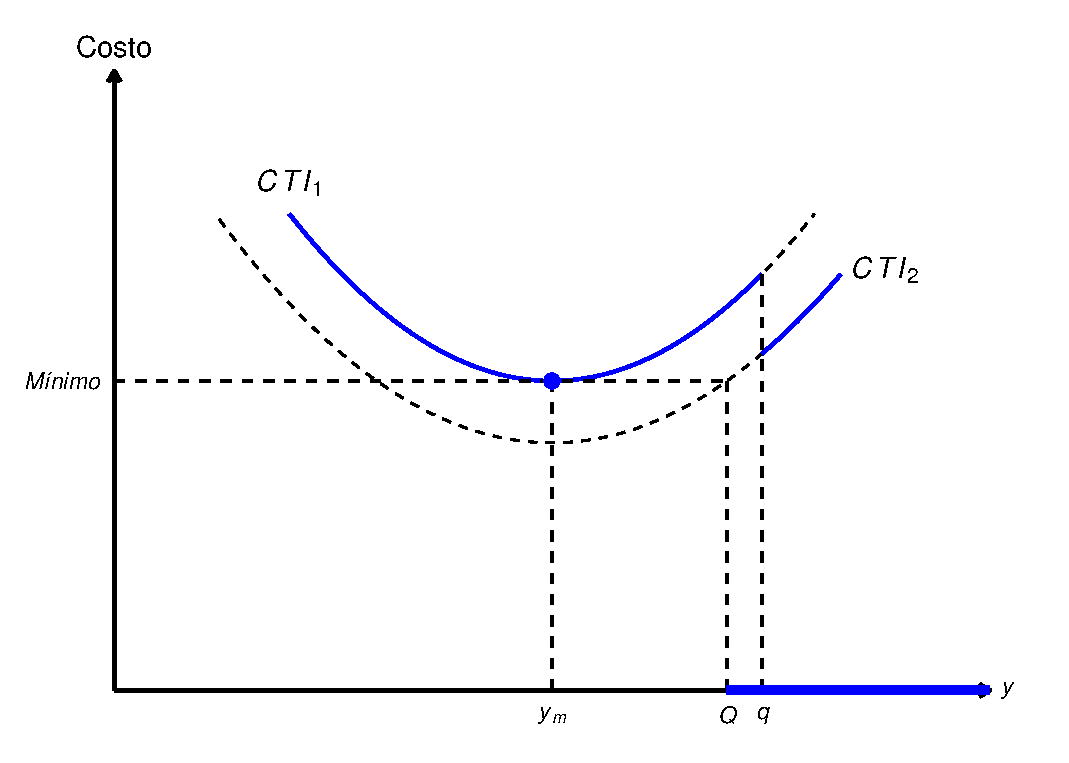
\includegraphics[width=13cm, height=6.1cm]{images/img6.pdf}
        \label{fig:img4c}
    \end{subfigure}
    \label{fig:img4}
\end{figure}

\newpage
\manualsubsubsection{2.2.15.3}{Modelo clásico de cantidad económica de pedido (EOQ) de varios productos con limitación de almacén}
En este modelo se considera que cada producto sigue el comportamiento del modelo clásico (EOQ) sin faltantes que se muestra en la Figura \ref{fig:img1}. Además se consideran que se tiene $n$ productos tal que $n>1$, entonces además de que los productos se utilizan con una demanda constante, a su vez tienen un espacio de almacenamiento con un límite de capacidad.

Definimos para cada producto $i$ tal que $i = 1, 2, \cdots , n$ sus respectivos
\begin{itemize}
	\item[$D_i=$] Tasa de demanda del producto $i$.
	\item[$K_i=$] Costo de preparación del producto $i$.
	\item[$h_i=$] Costo de retención del producto $i$.
	\item[$y_i=$] Cantidad de pedido del producto $i$.
	\item[$a_i=$] Espacio de almacenamiento para el producto $i$.
	\item[$A=$] Espacio de almacenamiento disponible para los $n$ productos.
\end{itemize}
Al igual que el modelo (EOQ) para cada producto $i$ en el que $i = 1, \cdots, n$ hallamos la duración del ciclo de pedido mediante la expresión (\ref{T}) quedando de la siguiente manera
\begin{equation}
	\label{T_i}
	{T}_{i} = \frac{y_i}{D_i}
\end{equation}
Cantidad de pedido óptima $y^*$ de la expresión (\ref{yopt}) para cada producto $i$
\begin{equation}
	\label{yiast}
	{y}_{i}^{*} = \sqrt{\frac{2{K}_{i}{D}_{i}}{{h}_{i}}}
\end{equation}
De igual forma para obtener el costo total de inventario $CTI(y)$ que se observa en la ecuación (\ref{CTI})
$$
CTI(y) = \frac{KD}{y} + DC + \frac{hy}{2}
$$
Para cada producto $i$ se borra el costo fijo $DC$ de donde $C$ es el costo por unidad del producto, ya que este no es el mismo al costo total al variar por producto, de tal forma que para cada producto el costo mínimo total quedaría de la siguiente forma:
\begin{equation}
	\label{CTI_i_opt}
	CTI({y}_{i}) = \frac{{K}_{i}{D}_{i}}{{y}_{i}} + \frac{{h}_{i}{y}_{i}}{2} 	
\end{equation} 
Y el costo mínimo total estaría dado por la siguiente función
\begin{eqnarray}
	CTI({y}_{1},{y}_{2},\cdots , {y}_{n}) &=& CTI({y}_{1}) + CTI({y}_{2}) + \cdots + CTI({y}_{n}) \nonumber \\
	 CTI({y}_{1},{y}_{2},\cdots , {y}_{n}) &=& \left(\frac{{K}_{1}{D}_{1}}{{y}_{1}} + \frac{{h}_{1}{y}_{1}}{2} 	 \right) + \left(\frac{{K}_{2}{D}_{2}}{{y}_{2}} + \frac{{h}_{2}{y}_{2}}{2} 	 \right) + \cdots + \left(\frac{{K}_{n}{D}_{n}}{{y}_{n}} + \frac{{h}_{n}{y}_{n}}{2} 	 \right) \nonumber \\
	 CTI({y}_{1},{y}_{2},\cdots , {y}_{n}) &=& \sum\limits_{i = 1}^{n} \left(\frac{{K}_{i}{D}_{i}}{{y}_{i}} + \frac{{h}_{i}{y}_{i}}{2} \right)
\end{eqnarray}
Tomando en cuenta de que el modelo no va a tener faltantes, el modelo matemático que exprese el inventario vendría a ser
$$
	\textsl{Minimizar }CTI({y}_{1},{y}_{2},\cdots , {y}_{n}) = \sum\limits_{i = 1}^{n} \left(\frac{{K}_{i}{D}_{i}}{{y}_{i}} + \frac{{h}_{i}{y}_{i}}{2} \right)
$$
Sujeto a
$$
\sum\limits_{i = 1}^{n} {a}_{i} {y}_{i} \leq A
$$
$$
{y}_{i} > 0, i = 1, 2, \cdots , n
$$
Primeramente se debe abordar el caso no restringido
$$
{y}_{i}^{*} = \sqrt{\frac{2{K}_{i}{D}_{i}}{{h}_{i}}}, i = 1, 2, \cdots , n
$$
Si la solución satisface la restricción, entonces el proceso termina. Caso contrario la restricción debe ser activada, uno de los métodos de activación es el método clásico de Lagrange (\ref{Mult_Lagrange}). Entonces el lagrangiano de la función es:
\begin{eqnarray}
	\label{funcion_lagrange}
	L(\lambda, {y}_{1}, {y}_{2}, \cdots , {y}_{n}) &=& CTI({y}_{1}, {y}_{2}, \cdots , {y}_{n}) - \lambda \left( \sum\limits_{i = 1}^{n} {a}_{i} {y}_{i} - A \right) \nonumber \\
	L(\lambda, {y}_{1}, {y}_{2}, \cdots , {y}_{n}) &=& \sum\limits_{i = 1}^{n} \left(\frac{{K}_{i}{D}_{i}}{{y}_{i}} + \frac{{h}_{i}{y}_{i}}{2} \right) - \lambda \left( \sum\limits_{i = 1}^{n} {a}_{i} {y}_{i} - A \right)
\end{eqnarray}
En donde $\lambda < 0$ es el multiplicador de Lagrange, asimismo la función de Lagrange es convexa, los valores óptimos de $y_i$ y $\lambda$ que minimizan a (\ref{funcion_lagrange}) se determina resolviendo el sistema
\begin{eqnarray}
	\label{lagran_yi}
	\frac{\partial L}{\partial {y}_{i}} = \frac{\partial}{\partial {y}_{i}} \left[ \sum\limits_{i = 1}^{n} \left(\frac{{K}_{i}{D}_{i}}{{y}_{i}} + \frac{{h}_{i}{y}_{i}}{2} \right) - \lambda \left( \sum\limits_{i = 1}^{n} {a}_{i} {y}_{i} - A \right) \right] = 0 \\
	\label{lagran_lambda}
	\frac{\partial L}{\partial \lambda} = \frac{\partial}{\partial \lambda} \left[ \sum\limits_{i = 1}^{n} \left(\frac{{K}_{i}{D}_{i}}{{y}_{i}} + \frac{{h}_{i}{y}_{i}}{2} \right) - \lambda \left( \sum\limits_{i = 1}^{n} {a}_{i} {y}_{i} - A \right) \right] = 0
\end{eqnarray}
De lo que resolviendo la primera derivada parcial (\ref{lagran_yi}) se tiene la siguiente expresión
\begin{eqnarray}
	\frac{\partial L}{\partial {y}_{i}} &=& - \frac{{K}_{i} {D}_{i}}{{y}_{i}^2} + \frac{{h}_{i}}{2} - \lambda {a}_{i} \nonumber
\end{eqnarray}
Esta expresión igualamos a cero y hallamos la cantidad de pedido óptimo ${y}_{i}^{*}$
\begin{eqnarray}
	\label{yi_opt_ast}
	- \frac{{K}_{i} {D}_{i}}{{y}_{i}^2} + \frac{{h}_{i}}{2} - \lambda {a}_{i} &=& 0 \nonumber \\
	\frac{{K}_{i} {D}_{i}}{{y}_{i}^2} &=& \frac{{h}_{i}}{2} - \lambda {a}_{i} \nonumber \\
	\frac{{K}_{i} {D}_{i}}{{y}_{i}^2} &=& \frac{{h}_{i} - 2 \lambda {a}_{i}}{2} \nonumber \\
	2 {K}_{i} {D}_{i} &=& {y}_{i}^{2} ({h}_{i} - 2 \lambda {a}_{i}) \nonumber \\
	{y}_{i}^{2} &=& \frac{2 {K}_{i} {D}_{i}}{{h}_{i} - 2 \lambda {a}_{i}} \nonumber \\
	{y}_{i} &=& \pm \sqrt{\frac{2 {K}_{i} {D}_{i}}{{h}_{i} - 2 \lambda {a}_{i}}} \quad \text{(solo se considera la parte positiva)} \nonumber \\
	{y}_{i}^{*} &=& \sqrt{\frac{2 {K}_{i} {D}_{i}}{{h}_{i} - 2 \lambda {a}_{i}}}
\end{eqnarray}
De igual forma resolviendo la derivada parcial (\ref{lagran_lambda}) se tiene la siguiente expresión
\begin{eqnarray}
	\frac{\partial L}{\partial \lambda} &=& A - \sum\limits_{i = 1}^{n} {a}_{i} {y}_{i} \nonumber
\end{eqnarray}
Ahora igualando a cero y reemplazando ${y}_{i}$ por el valor de ${y}_{i}^{*}$ de (\ref{yi_opt_ast}) se tiene
\begin{eqnarray}
	\label{lagran_lambda2}
	A - \sum\limits_{i = 1}^{n} {a}_{i} {y}_{i} &=& 0 \nonumber \\
	A - \sum\limits_{i = 1}^{n} {a}_{i} \sqrt{\frac{2 {K}_{i} {D}_{i}}{{h}_{i} - 2 \lambda {a}_{i}}} &=& 0 
\end{eqnarray}
Si $\lambda = 0$ en la expresión (\ref{yi_opt_ast}) se tiene la cantidad de pedido óptima $y^*$ igual a (\ref{yiast}), por lo que se debe tener un valor de $\lambda < 0$ para que cumpla la igualdad de (\ref{lagran_lambda2}) si no es así se vuelve a repetir el proceso asignando otro valor negativo $\lambda$ hasta lograr una aproximación a la igualdad (\ref{lagran_lambda2}).

\manualsubsubsection{2.2.15.4}{Modelo clásico de cantidad económica de pedido (EOQ) con escasez}\label{EOQ_escasez}
Uno de los problemas más grandes que se tienen en los modelos de inventarios son los faltantes, que es cuando la demanda no se satisface y genera retrasos, esto es debido a que el inventario agoto los productos en existencia hasta volver a reabastecerse, los casos en donde se permiten estos faltantes es cuando el cliente acepta este retraso si es necesario, donde se toma el riesgo de la pérdida del cliente o la caída del negocio. Este modelo toma en consideración estos casos extendiendo el modelo clásico (EOQ) que se observa en la Figura \ref{fig:img1} donde:
\begin{itemize}
	\item[$S=$] Nivel del inventario después de recibir $y$ unidades.
	\item[$y-S=$] Escasez del inventario antes de recibir $y$ unidades.
	\item[$t_1=$] Intervalo de tiempo en el cual el inventario no es negativo y satisface la demanda.
	\item[$t_2=$] Intervalo de tiempo en el cual el inventario es negativo y no satisface la demanda.
\end{itemize}
El comportamiento del modelo clásico de cantidad económica de pedido con escasez se observa en la Figura \ref{fig:imga}.
\newpage
\begin{figure}[H]
  \caption{Modelo clásico económica de pedido (EOQ) con demanda diferida}
  {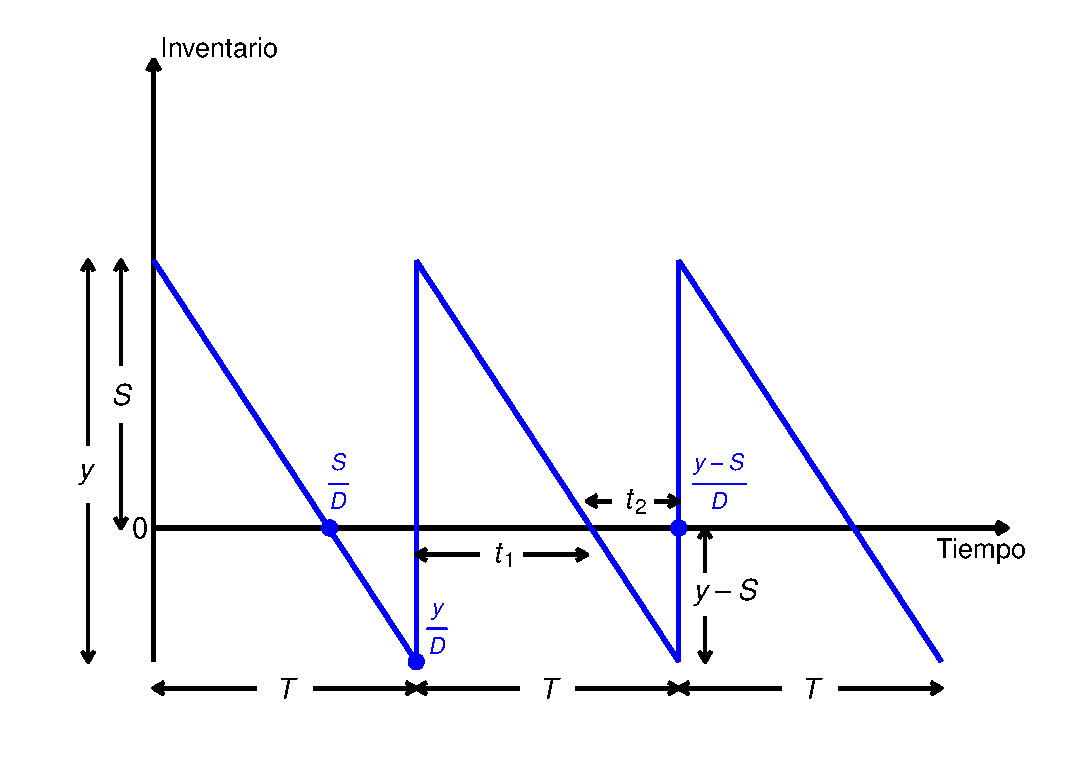
\includegraphics[width=15cm, height=7.7cm]{images/imga.pdf}}
  \label{fig:imga}
\end{figure}
En la cual por semejanza de triángulos podemos hallar el intervalo de tiempo que satisface la demanda:
\begin{eqnarray}
	\frac{t_1}{T} &=& \frac{S}{y} \nonumber \\
	t_1 &=& \frac{S}{y}T \nonumber
\end{eqnarray}
A esta expresión reemplazemos el valor $T$ de (\ref{T})
\begin{eqnarray}
	t_1 &=& \frac{S}{y} \left( \frac{y}{D} \right) \nonumber \\
	t_1 &=& \frac{S}{D}
\end{eqnarray}
De igual forma por semejanza de triángulos hallamos el intervalo en donde no se satisface la demanda:
\begin{eqnarray}
	\frac{t_2}{T} &=& \frac{y-S}{y} \nonumber \\
	t_2 &=& \frac{y-S}{y}(T) \nonumber
\end{eqnarray}
\newpage
\noindent De la misma forma reemplazamos $T$ de (\ref{T})
\begin{eqnarray}
	t_2 &=& \frac{y-S}{y} \left( \frac{y}{D} \right) \nonumber \\
	t_2 &=& \frac{y-S}{D}
\end{eqnarray}
Como se vieron en los anteriores casos para sacar el costo total del inventario $CTI(y)$ se tienen que tomar en cuenta el costo por producción en el intervalo de tiempo ($CPT$) enunciada en la expresión (\ref{CPT}). El costo de almacenamiento por intervalo de tiempo $(CAIT)$ se da solo en el tiempo $\frac{S}{D}$ por lo que extendiendo la expresión (\ref{CAIT}) reemplazando ``$y$'' por $S$ se tiene la siguiente expresión
\begin{equation}
	\label{CAITescasez}
	CAIT = \frac{hS^2}{2D}
\end{equation}
Ahora el déficit del inventario ocurre en un intervalo de tiempo $\frac{y-S}{D}$ en donde se tiene un costo de escasez ``$p$'', de la misma analogía que (\ref{CAIT}) se tiene la siguiente expresión para el costo de escasez por intervalo de tiempo $(CET)$
\begin{equation}
	\label{CETescasez}
	CET = \frac{p{(y-S)}^{2}}{2D} 	
\end{equation} 
De lo que el costo total por intervalo de tiempo $(CTT)$ estaría en función de la adición del costo de almacenamiento $(CAIT)$, el costo de producción $(CPT)$ y el costo por escasez $(CET)$ por intervalo de tiempo
\begin{equation}
	CTT = CPT + CAIT + CET
\end{equation}
Reemplazando los valores $(CPT)$, $(CAIT)$ y $(CET)$ por las expresiones (\ref{CPT}), (\ref{CAITescasez}) y (\ref{CETescasez}) respectivamente se tiene la siguiente expresión
\begin{equation}
	CTT = K + Cy + \frac{hS^2}{2D} + \frac{p{(y-S)}^{2}}{2D}
\end{equation}
De la misma forma que se realizó en (\ref{CTIdejado}) dividimos el $(CTT)$ por el tiempo $(T)$, y reemplazando $T$ por la expresión (\ref{T}), se tiene el costo total del inventario del modelo con demanda diferida.
\begin{eqnarray}
	\label{CTIy_esc_fal}
	CTI(y) &=& \frac{CTT}{T} \nonumber \\
	CTI(y) &=& \frac{K + Cy + \frac{hS^2}{2D} + \frac{p{(y-S)}^{2}}{2D}}{T} \nonumber \\
	CTI(y) &=& \frac{K + Cy + \frac{hS^2}{2D} + \frac{p{(y-S)}^{2}}{2D}}{\frac{y}{D}} \nonumber \\
%\end{eqnarray}
%\begin{eqnarray}
	CTI(y) &=& \frac{\frac{2DK + 2DCy + hS^2 + p{(y-S)}^{2}}{2D}}{\frac{y}{D}} \nonumber \\
	CTI(y) &=& \frac{2DK + 2DCy + hS^2 + p{(y-S)}^{2}}{2y} \nonumber \\
	CTI(y) &=& \frac{DK}{y} + DC + \frac{hS^2}{2y}+\frac{p{(y-S)}^{2}}{2y}
\end{eqnarray}
Para este caso en la expresión (\ref{CTIy_esc_fal}) se tienen dos variables de decisión ``$S$'' y ``$y$'', en lo cual para encontrar los valores óptimos $S^*$ y $y^*$ se halla el vector gradiente $\nabla CTI(y)$ con las respectivas derivadas parciales e igualando a cero, teniendo el siguiente sistema
\begin{eqnarray}
	\label{part1}
	\frac{\partial CTI(y)}{\partial S} &=& \frac{\partial}{\partial S} \left[ \frac{DK}{y} + DC + \frac{hS^2}{2y}+\frac{p{(y-S)}^{2}}{2y} \right] = 0 \\
	\label{part2}
	\frac{\partial CTI(y)}{\partial y} &=& \frac{\partial}{\partial y} \left[ \frac{DK}{y} + DC + \frac{hS^2}{2y}+\frac{p{(y-S)}^{2}}{2y} \right] = 0
\end{eqnarray}
Resolviendo (\ref{part1}) se tiene que:
\begin{eqnarray}
	\label{2_40}
	\frac{\partial CTI(y)}{\partial S} &=& \frac{\partial}{\partial S} \left[ \frac{DK}{y} + DC + \frac{hS^2}{2y}+\frac{p{(y-S)}^{2}}{2y} \right] \nonumber \\
	\frac{\partial CTI(y)}{\partial S} &=& \frac{2hS}{2y} + \frac{2p(y-S)(-1)}{2y} \nonumber \\
	\frac{\partial CTI(y)}{\partial S} &=& \frac{hS}{y} - \frac{p(y-S)}{y}
\end{eqnarray}
Ahora igualando (\ref{2_40}) a cero se tiene el valor para $S$ 
\begin{eqnarray}
	\label{S_240}
	\frac{hS}{y} - \frac{p(y-S)}{y} &=& 0 \nonumber \\
	\frac{hS - p (y-S)}{y} &=& 0 \nonumber \\
	hS &=& p(y-S) \nonumber \\
	hS &=& py - pS \nonumber \\
	hS + pS &=& py \nonumber \\
	S(h+p) &=& py \nonumber \\
	S &=& \frac{py}{h+p}
\end{eqnarray}
De la misma forma resolviendo (\ref{part2}) se tiene que:
\begin{eqnarray}
	\label{2_41}
	\frac{\partial CTI(y)}{\partial y} &=& \frac{\partial}{\partial y} \left[ \frac{DK}{y} + DC + \frac{hS^2}{2y}+\frac{p{(y-S)}^{2}}{2y} \right] \nonumber \\
	\frac{\partial CTI(y)}{\partial y} &=& - \frac{DK}{y^2} - \frac{hS^2}{2y^2} + \frac{2y[2p(y-S)]-[p{(y-S)}^{2}]2}{4y^2} \nonumber \\
	\frac{\partial CTI(y)}{\partial y} &=& - \frac{DK}{y^2} - \frac{hS^2}{2y^2} + \frac{4py(y-S)-2p{(y-S)}^{2}}{4y^2} \nonumber \\
	\frac{\partial CTI(y)}{\partial y} &=& - \frac{DK}{y^2} - \frac{hS^2}{2y^2} + \frac{2p(y-S)(2y-(y-S))}{4y^2} \nonumber \\
	\frac{\partial CTI(y)}{\partial y} &=& - \frac{DK}{y^2} - \frac{hS^2}{2y^2} + \frac{2p(y-S)(y+S)}{4y^2} \nonumber \\
	\frac{\partial CTI(y)}{\partial y} &=& - \frac{DK}{y^2} - \frac{hS^2}{2y^2} + \frac{p(y^2 - S^2)}{2y^2} \nonumber \\
	\frac{\partial CTI(y)}{\partial y} &=& - \frac{DK}{y^2} - \frac{hS^2}{2y^2} + \frac{py^2 - pS^2}{2y^2} \nonumber \\
	\frac{\partial CTI(y)}{\partial y} &=& - \frac{DK}{y^2} - \frac{hS^2}{2y^2} + \frac{py^2}{2y^2} - \frac{pS^2}{2y^2} \nonumber \\
	\frac{\partial CTI(y)}{\partial y} &=& - \frac{DK}{y^2} + \frac{p}{2} - \frac{hS^2}{2y^2} - \frac{pS^2}{2y^2} \nonumber \\
	\frac{\partial CTI(y)}{\partial y} &=& - \frac{DK}{y^2} + \frac{p}{2} - \frac{(h + p)}{2y^2}S^2
\end{eqnarray}
Ahora igualando (\ref{2_41}) a cero y reemplazando $S$ por el valor de (\ref{S_240})  se tiene el valor para la cantidad de pedido óptima $y^*$
\newpage
\begin{eqnarray}
		\label{y_ast}
	 	- \frac{DK}{y^2} + \frac{p}{2} - \frac{(h + p)}{2y^2}S^2 &=& 0 \nonumber \\
	 	- \frac{DK}{y^2} + \frac{p}{2} - \frac{(h + p)}{2y^2} {\left(\frac{py}{h+p} \right)}^{2} &=& 0 \nonumber \\
	 	- \frac{DK}{y^2} + \frac{p}{2} - \frac{p^2}{2(h+p)} &=& 0 \nonumber \\
	 	- \frac{DK}{y^2} + \frac{p(h+p)-p^2}{2(h+p)} &=& 0 \nonumber \\
	 	- \frac{DK}{y^2} + \frac{ph}{2(h+p)} &=& 0 \nonumber \\
	 	y^2 &=& \frac{2(h+p)DK}{ph} \nonumber \\
	 	y^2 &=& \left( \frac{2DK}{h} \right) \left( \frac{h+p}{p} \right) \nonumber \\
	 	y &=& \pm \sqrt{\left( \frac{2DK}{h} \right) \left( \frac{h+p}{p} \right)} \quad \text{(solo se considera la parte positiva)} \nonumber \\
	 	y^* &=& \sqrt{\frac{2DK}{h}} \sqrt{\frac{h+p}{p}}
\end{eqnarray}
De la misma forma reemplazamos $y^*$ de (\ref{y_ast}) en (\ref{S_240}) para obtener el nivel de inventario óptimo $(S^*)$ para recibir las cantidades de pedido óptimas.
\begin{eqnarray}
	\label{S_ast}
	S^* &=& \frac{py^*}{h+p} \nonumber \\
	S^* &=& \left(\frac{p}{h+p} \right) \sqrt{\frac{2DK}{h}} \sqrt{\frac{h+p}{p}} \nonumber \\
	S^* &=& \sqrt{\frac{(p^2)(2DK)(h+p)}{{(h+p)}^{2}hp}} \nonumber \\
	S^* &=& \sqrt{\frac{2DKp}{h(h+p)}} \nonumber \\
	S^* &=& \sqrt{\frac{2DK}{h}}\sqrt{\frac{p}{h+p}}
\end{eqnarray}
El tiempo de ciclo en cada pedido óptimo $(T^*)$ estaría expresado en base a (\ref{T}) reemplanzando por el valor de $y$ por $y^*$ de (\ref{y_ast})
\newpage
\begin{eqnarray}
	T^* &=& \frac{y^*}{D} \nonumber \\
	T^* &=& \frac{1}{D} \sqrt{\frac{2DK}{h}} \sqrt{\frac{h+p}{p}} \nonumber \\
	T^* &=& \sqrt{\frac{2DK(h+p)}{D^2 hp}} \nonumber \\
	T^* &=& \sqrt{\frac{2K}{Dh}} \sqrt{\frac{(h+p)}{p}}
\end{eqnarray}
La escasez del inventario óptima $(y^* - S^*)$ antes de recibir las $y^*$ unidades estaría en función de reemplazar $y$ por (\ref{y_ast}) y $S$ por (\ref{S_ast})
\begin{eqnarray}
	y^* - S^* &=& \sqrt{\frac{2DK}{h}} \sqrt{\frac{h+p}{p}} - \sqrt{\frac{2DK}{h}}\sqrt{\frac{p}{h+p}} \nonumber \\
	y^* - S^* &=& \sqrt{\frac{2DK}{h}} \left( \sqrt{\frac{h+p}{p}} - \sqrt{\frac{p}{h+p}} \right) \nonumber \\
	y^* - S^* &=& \sqrt{\frac{2DK}{h}} \left( \frac{{(\sqrt{h+p})}^{2} - {(\sqrt{p})}^{2}}{\sqrt{p(h+p)}}  \right) \nonumber \\
	y^* - S^* &=& \sqrt{\frac{2DK}{h}} \left( \frac{h}{\sqrt{p(h+p)}}  \right) \nonumber \\
	y^* - S^* &=& \sqrt{\frac{2DKh^2}{hp(h+p)}} \nonumber \\
	y^* - S^* &=& \sqrt{\frac{2DK}{p}} \sqrt{\frac{h}{(h+p)}}
\end{eqnarray}
Por último, de igual forma hallemos el total de inventario de la expresión (\ref{CTIy_esc_fal})
\begin{eqnarray}
	\label{CTI_escasezz}
	CTI(y) &=& \frac{DK}{y} + DC + \frac{hS^2}{2y}+\frac{p{(y-S)}^{2}}{2y} \nonumber \\
	CTI(y) &=& \frac{2DK + hS^2 + p{(y-S)}^{2}}{2y} + DC \nonumber \\
	CTI(y) &=& \frac{2DK + hS^2 + py^2 - 2pyS + pS^2}{2y} + DC \nonumber \\
	CTI(y^*) &=& \frac{2DK + (h+p){S}^{2} + p{y}^{2} - 2pyS}{2y} + DC
\end{eqnarray}
A la expresión reemplazemos los valores de $y$ y $S$ por los valores de $y^*$ y $S^*$ de las expresiones (\ref{y_ast}) y (\ref{S_ast}) respectivamente en la expresiòn (\ref{CTI_escasezz}) para hallar el costo mínimo total del inventario $CTI(y^*)$
\begin{eqnarray}
	CTI(y^*) &=& \frac{2DK + (h+p){S^*}^{2} + p{y^*}^{2} - 2py^*S^*}{2y^*} + DC \nonumber \\
	CTI(y^*) &=& \frac{2DK + (h+p){\left( \sqrt{\frac{2DK}{h}}\sqrt{\frac{p}{h+p}} \right)}^{2} + p{\left( \sqrt{\frac{2DK}{h}} \sqrt{\frac{h+p}{p}} \right)}^{2} - 2p\left( \sqrt{\frac{2DK}{h}} \sqrt{\frac{h+p}{p}} \right) \left( \sqrt{\frac{2DK}{h}}\sqrt{\frac{p}{h+p}} \right)}{2\left( \sqrt{\frac{2DK}{h}} \sqrt{\frac{h+p}{p}} \right)} + DC \nonumber \\
	CTI(y^*) &=& \frac{2DK + (h+p)\left( \frac{2DKp}{h(h+p)} \right) + p \left( \frac{2DK(h+p)}{hp} \right) - 2p \left( \sqrt{\frac{p{(2DK)}^{2}(h+p)}{h^2 p (h+p)}} \right) }{2 \left(\sqrt{\frac{2DK(h+p)}{hp}} \right)} + DC \nonumber \\
	CTI(y^*) &=& \frac{2DK + \frac{2DKp}{h}  + \frac{2DK(h+p)}{h} - 2p \left( \frac{2DK}{h} \right) }{2 \left(\sqrt{\frac{2DK(h+p)}{hp}} \right)} + DC \nonumber \\
	CTI(y^*) &=& \frac{2 \left( DK + \frac{DKp}{h}  + \frac{DK(h+p)}{h} - \frac{2DKp}{h} \right) }{2 \left(\sqrt{\frac{2DK(h+p)}{hp}} \right)} + DC \nonumber \\
	CTI(y^*) &=& \frac{\frac{DKh + DKp + DKh + DKp - 2DKp}{h}}{\sqrt{\frac{2DK(h+p)}{hp}}} + DC \nonumber \\
	CTI(y^*) &=& \frac{\frac{2DKh}{h}}{\sqrt{\frac{2DK(h+p)}{hp}}} + DC \nonumber \\
	CTI(y^*) &=& \sqrt{\frac{4D^2 K^2 h^2 hp}{h^2 2DK (h+p)}} + DC \nonumber \\
	CTI(y^*) &=& \sqrt{\frac{2DKhp}{h+p}} + DC \nonumber \\
	CTI(y^*) &=& \sqrt{2DKh} \sqrt{\frac{p}{h+p}} + DC
\end{eqnarray}
De la misma forma que se realizó en (\ref{yopt}) para demostrar que el valor es mínimo se realiza la prueba de la segunda derivada a la expresión del costo total de inventario $CTI(y)$ con respecto a ``$y$'' y ``$S$''
\newpage
\begin{eqnarray}
	\label{minimo2}
	\frac{d^2 CTI(y)}{dy^2} &=& \frac{d^2}{dy^2} \left[ \frac{DK}{y} + DC + \frac{hS^2}{2y}+\frac{p{(y-S)}^{2}}{2y} \right] \nonumber \\
	\frac{d^2 CTI(y)}{dy^2} &=& \frac{d}{dy} \left( - \frac{DK}{y^2} + \frac{p}{2} - \frac{(h + p)}{2y^2}S^2 \right) \nonumber \\
	\frac{d^2 CTI(y)}{dy^2} &=& \frac{2KD + (h+p)S^2}{y^3} \geq 0; \quad \forall y \\
	\frac{d^2 CTI(y)}{dS^2} &=& \frac{d^2}{dS^2} \left[ \frac{DK}{y} + DC + \frac{hS^2}{2y}+\frac{p{(y-S)}^{2}}{2y} \right] \nonumber \\
	\frac{d^2 CTI(S)}{dS^2} &=& \frac{d}{dS} \left( \frac{hS}{y} - \frac{p(y-S)}{y} \right) \nonumber \\
	\frac{d^2 CTI(S)}{dS^2} &=& \frac{h+p}{y} \geq 0; \quad \forall S
\end{eqnarray}
%Y de la misma forma que se realizó en (\ref{convexo1}) del teorema (\ref{convexo_dos_derivadas}) se demuestra la convexidad puesto que
%\begin{equation}
%	\label{convexo2}
%	\frac{d^2 CTI(y)}{dy^2} = \frac{2KD + (h+p)S^2}{y^3} < 0; \quad \forall y > 0
%\end{equation}
%La función $CTI(y)$ es convexa en $(0, + \infty)$, por lo que $y^*$ es el minimo de la función.
%--------------------------------------------
%----------- MODELOS PROBABILISTICOS ---------
%--------------------------------------------
\subsection{Modelos de inventario probabilísticos o estocásticos}
A diferencia del modelo determinístico presentado en la sección anterior, en este tipo de modelos se analizan los inventarios con un desconocimiento sobre la demanda para los periodos siguientes, aunque estos pueden ser representados como una variable aleatoria que siga una distribución de probabilidad conocida. \citep{taha2012investigacion}

Primeramente se explicarán los modelos con revisión continua que tienen dos modelos, la versión probabilística del modelo clásico (EOQ) y el modelo (EOQ) probabilizado que tiene una demanda aleatoria. Seguidamente se explicarán los modelos de revisión periódica como los modelos de un periodo sin costo de preparación, con costo de preparación y los modelos de varios periodos. 
\manualsubsubsection{2.2.16.1}{Modelo probabilizado de cantidad económica de pedido}\label{EOQ_probabilizado}
Son algunos los profesionales que buscaron la forma de adaptar el modelo EOQ determinístico para explicar de manera aproximada la naturaleza probabilística de la demanda. Se tiene un problema de periodo crítico en el ciclo del inventario entre la colocación y recepción de pedidos que pueda ocasionar que no se tengan los productos. Por lo que se toma la idea de tener la probabilidad de tener pocos faltantes y mayores reservas. Donde se tienen las siguientes variables:
\begin{itemize}
	\item[$B=$] Cantidad de la existencia de reserva.
	\item[$L=$] Tiempo de espera entre la llegada del producto y su siguiente colocación.
	\item[${x}_{L}=$] Variable aleatoria de la demanda durante el tiempo de espera $L$.
	\item[${\mu}_{L}=$] Media de la demanda en el tiempo de espera $L$.
	\item[${\sigma}_{L}=$] Desviación estándar de la demanda en el tiempo de espera $L$.
	\item[${y}^{*}=$] Cantidad de pedido óptimo del modelo (EOQ).
	\item[$\alpha =$] Probabilidad máxima de admitir faltantes durante el tiempo de espera $L$.
	\item[$B + {\mu}_{L} =$] Punto de pedido según la media de la demanda y la cantidad de reserva.
\end{itemize}
La relación del modelo EOQ con respecto a las reservas se muestran en la Figura \ref{fig:EOQ_ext}.

\begin{figure}[H]
  \caption{Modelo clásico EOQ con existencias de reservas $B$}
  {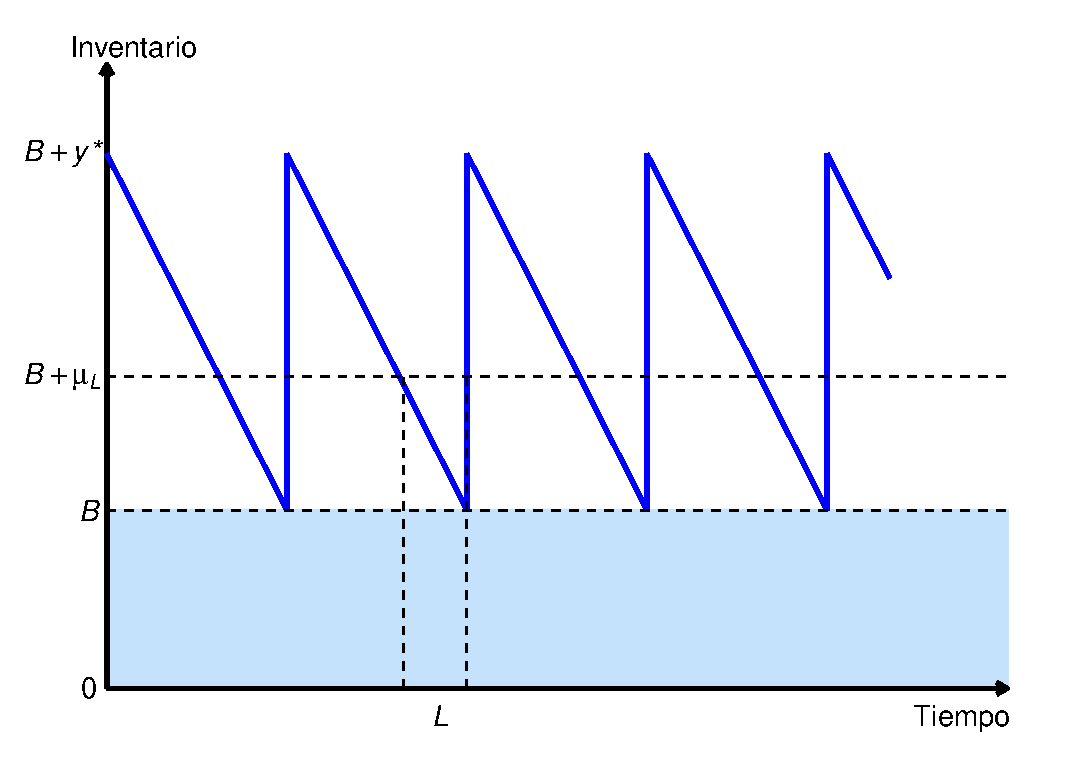
\includegraphics[width=15cm, height=8.5cm]{images/EOQ_ext.pdf}}
  \label{fig:EOQ_ext}
\end{figure} 

La hipótesis planteada del modelo es que la demanda por unidad de tiempo sigue una distribución normal con media $D$ y desviación estándar $\sigma$, denotado como $N(D,\sigma)$. Generalizando la definición de distribución normal mostrado en la subsección (\ref{Dist_normal}) expresando la demanda como una variable aleatoria durante un tiempo de espera $L$, en lo cual debe seguir la distribución de probabilidad normal con media ${\mu}_{L} = DL$ y desviación estándar ${\sigma}_{L} = \sqrt{L {\sigma}^{2}}$, representado de la siguiente manera ${x}_{L} \sim N({\mu}_{L},{\sigma}_{L})$. La definición de $L$ es la misma del modelo clásico en (\ref{Modelo_clas_EOQ}).
La cantidad de existencia de reservas $B$ se determina mediante la probabilidad de faltantes durante $L$ sea a lo máximo $\alpha$ de la siguiente forma:
\begin{equation}
	\label{eq:Prob1}
	P[ {x}_{L} \geq B + {\mu}_{L} ] \leq \alpha
\end{equation}
De lo cual a la expresión (\ref{eq:Prob1}) si despejamos con respecto a $B$ y estandarizamos se tiene la siguiente expresión:
\begin{eqnarray}
	\label{eq:Prob2}
	P[ {x}_{L} - {\mu}_{L} \geq B  ] &\leq& \alpha \nonumber \\
	P \left[ \frac{{x}_{L} - {\mu}_{L}}{{\sigma}_{L}} \geq \frac{B}{{\sigma}_{L}} \right] &\leq& \alpha \nonumber \\
	P \left[ z \geq \frac{B}{{\sigma}_{L}} \right] &\leq& \alpha 
\end{eqnarray}
De (\ref{eq:Prob2}) se tiene que $z = \frac{{x}_{L} - {\mu}_{L}}{{\sigma}_{L}}$ es la estandarización de ${x}_{L}$ que sigue una distribución normal estándar $N(0,1)$. Se define el parámetro ${K}_{\alpha}$ para la distribución normal estándar de modo que $P[z \geq {k}_{\alpha}] \leq \alpha$ que se observa en la Figura \ref{fig:img10}.
\begin{figure}[H]
  \caption{Probabilidad de que se agoten las reservas $P[z \leq {K}_{\alpha}] = \alpha$}
  {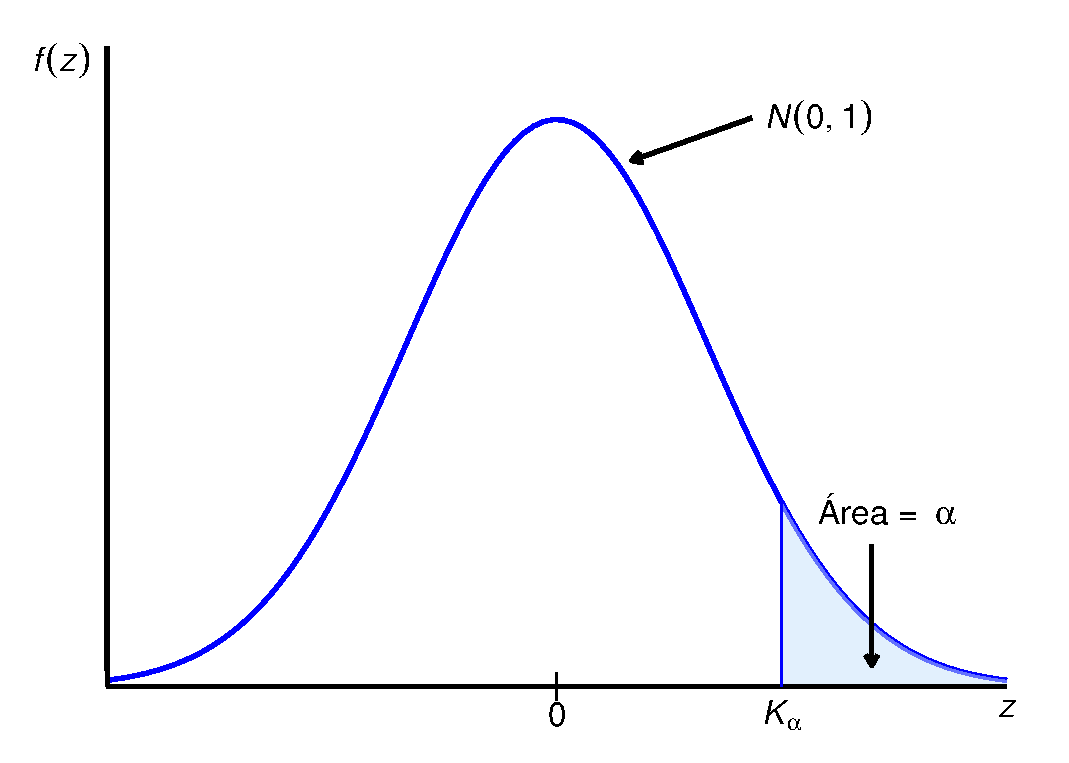
\includegraphics[width=15cm, height=7cm]{images/img10.pdf}}
  \label{fig:img10}
\end{figure} 
Por lo que el tamaño de reserva debe satisfacer la siguiente desigualdad
\newpage
\begin{equation}
	\label{eq:Prob3}
	B \leq {\sigma}_{L} {K}_{\alpha}
\end{equation}
En el cual de (\ref{eq:Prob3}) se tiene que ${\sigma}_{L}{K}_{\alpha}$ proporciona el valor mínimo de $B$ y se requiere que $L$ sea un valor entero ya sea por el valor exacto o redondeando el valor.

\manualsubsubsection{2.2.16.2}{Modelo cantidad de pedido económica (EOQ) probabilístico}
El modelo probabilizado EOQ visto en la anterior sección no hace verosimil la producción de una política óptima, ya que se ignora el hecho de que la demanda tenga un comportamiento probabilístico. Por lo cual el modelo de cantidad de pedido económica (EOQ) probabilístico toma en cuenta el comportamiento probabilístico de la demanda. De igual forma la política del inventario establece en realizar el pedido de ``$y$'' cantidades cuando el inventario llegue al punto de reorden ``$R$'' que al igual que en el modelo determinístico tiene un tiempo entre el pedido y la recepción del pedido. Para encontrar los valores óptimos de ``$y$'' y ``$R$'' se debe minimizar la suma esperada de los costos de retención y los costos de faltantes por unidad de tiempo. El modelo toma en cuenta tres suposiciones:
\begin{enumerate}
	\item La demanda que no se satisface en el ciclo de espera se guardan o almacenan.
	\item No se debe permitir más de un pedido pendiente.
	\item La distribución de la demanda en el ciclo de espera es estacionaria con el tiempo.
\end{enumerate}
Asimismo la función de costo total por unidad de tiempo se toman en cuenta las siguientes variables:
\begin{itemize}
	\item[$f(x) =$] Función de densidad de probabilidad de la demanda ``$x$'' durante el ciclo de espera.
	\item[$D =$] Demanda esperada por unidad de tiempo.
	\item[$h =$] Costo de retención o almacenamiento del inventario por unidad de tiempo.
	\item[$p =$] Costo por escasez o faltante del inventario.
	\item[$K =$] Costo de preparación del pedido.
\end{itemize}
El comportamiento del modelo se puede observar en la Figura \ref{fig:img11}.
\begin{figure}[h!]
  \caption{Modelo de inventario probabilístico con faltante}
  {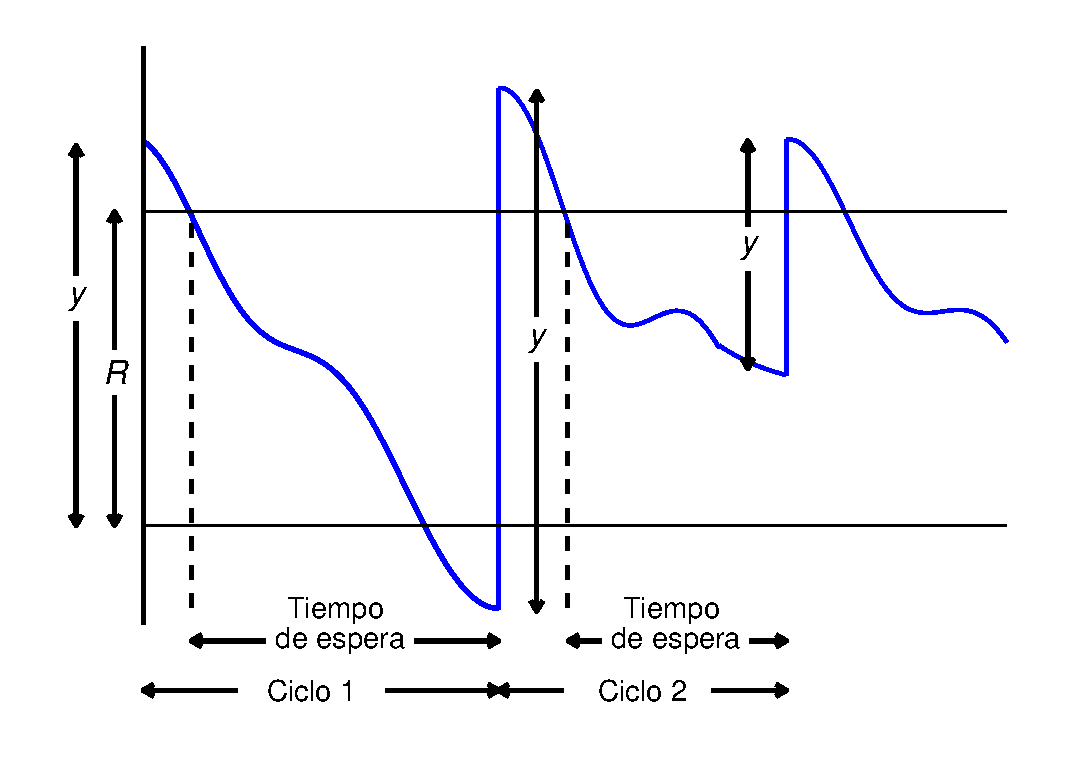
\includegraphics[width=15cm, height=7cm]{images/img11.pdf}}
  \label{fig:img11}
\end{figure} 
En el cual se observan que en los ciclos pueden ocurrir o no faltantes (tal vez con un comportamiento aleatorio), como en el ciclo 1 y 2 de la Figura \ref{fig:img11}. Con estas variables se determinan los elementos de la función de costos
\begin{enumerate}
	\item \textbf{Costo de preparación $(CPT)$:} Es la cantidad aproximada de pedidos por unidad de tiempo es $\frac{D}{y}$, de modo que el costo de preparación por unidad de tiempo es aproxidamente $\frac{KD}{y}$.
	\begin{equation}
		\label{prob:CPT}
		CPT = \frac{KD}{y}
	\end{equation}
	\item \textbf{Costo de retención esperado $(CRE)$:} Si $I$ es el nivel de inventario promedio, el costo de retención o almacenamiento pur unidad de tiempo es ``$hI$''. Para calcular $I$ se toma en cuenta el promedio de los inventarios esperados inicial y final de un ciclo es decir $y + E[R - x]$ y $E[R-x]$ respectivamente de la siguiente forma:
	\begin{eqnarray}
		\label{prob:I}
		I &=& \frac{(y + E[R-x])+E[R-x]}{2} \nonumber \\
		I &=& \frac{(y+E[R]-E[x])+E[R]-E[x]}{2} \nonumber \\
		I &=& \frac{y}{2} + 2\frac{(R-E[x])}{2} \nonumber \\
		I &=& \frac{y}{2} + R - E[x]
	\end{eqnarray}
	En el cual $R-E[x]$ se ignora que pueda ser negativo, ahora el costo de retención esperado $(CRE)$ estaría en función de $h$ e $I$ de la expresión (\ref{prob:I}) mediante la siguiente forma:
	\begin{eqnarray}
		\label{prob:CRE}
		CRE &=& hI \nonumber \\
		CRE &=& h \left( \frac{y}{2} + R - E[x] \right)
	\end{eqnarray}
	\item \textbf{Costo por faltanes esperado:} Los faltantes se dan en el caso que $x > R$. De lo cual tomando en cuenta una función de densidad (\ref{VAContinua}) su valor esperado en el ciclo se calcula como:
	\begin{equation}
		\label{prob:S}
		S = \int_{R}^{\infty} (x-R)f(x)dx
	\end{equation}
\end{enumerate}
Como el costo por escasez ``$p$'' es proporcional sólo a la cantidad faltante, el costo esperado por cada ciclo es $pS$ y tomando en cuenta $\frac{D}{y}$ ciclos por unidad de tiempo, el costo de escasez por unidad de tiempo $(CET)$ es:
\begin{eqnarray}
	\label{prob:CET}
	CET &=& \frac{pS}{T} \nonumber \\
	CET &=& \frac{pS}{\frac{y}{D}} \nonumber \\
	CET &=& \frac{pDS}{y}
\end{eqnarray}  
De lo cual el costo total del inventario $CTI$ es igual a la suma del costo de preparación $(CPT)$, costo de retención esperado $(CRE)$ y el costo de escasez $(CET)$ por unidad de tiempo de las expresiones (\ref{prob:CPT}), (\ref{prob:CRE}) y (\ref{prob:CET}) respectivamente. El cual estaría en función de ``$y$'' y ``$R$'' de la siguiente manera:
\begin{eqnarray}
	\label{prob:CTI_y_R}
	CTI(y,R) &=& CPT + CRE + CET \nonumber \\
	CTI(y,R) &=& \frac{DK}{y} + h \left( \frac{y}{2} + R - E[x] \right) + \frac{pDS}{y}
\end{eqnarray}
\newpage
Como se realizó antes las soluciones óptimas de $y^*$ y $R^*$ se determinan mediante las derivadas parciales e igualando a cero la expresión (\ref{prob:CTI_y_R}) mediante las siguientes ecuaciones:
\begin{eqnarray}
	\label{prob:CTI_y_der}
	\frac{\partial CTI(y,R)}{\partial y} &=& \frac{\partial}{\partial y} \left[\frac{DK}{y} + h \left(\frac{y}{2} + R - E[x] \right) + \frac{pDS}{y} \right] = 0 \\
	\label{prob:CTI_R_der}
	\frac{\partial CTI(y,R)}{\partial R} &=& \frac{\partial}{\partial R} \left[\frac{DK}{y} + h \left(\frac{y}{2} + R - E[x] \right) + \frac{pDS}{y} \right] = 0
\end{eqnarray}
De lo que resolviendo la primera derivada parcial (\ref{prob:CTI_y_der}) se tiene la siguiente expresión:
\begin{eqnarray}
	\frac{\partial CTI(y,R)}{\partial y} = - \frac{DK}{y^2} + \frac{h}{2} - \frac{pDS}{y^2} = 0 \nonumber
\end{eqnarray}
Esta expresión igualamos a cero y hallamos la cantidad de pedido óptima $y^*$
\begin{eqnarray}
	\label{prob:y_opt_int}
	- \frac{DK}{y^2} + \frac{h}{2} - \frac{pDS}{y^2} &=& 0 \nonumber \\
	-2DK + y^2 h - 2pDS &=& 0 \nonumber \\
	y^2 &=& \frac{2D(K + pS)}{h} \nonumber \\
	y &=& \pm \sqrt{\frac{2D(K+pS)}{h}} \quad \text{(solo se considera la parte positiva)} \nonumber \\
	y^* &=&  \sqrt{\frac{2D(K+pS)}{h}}
\end{eqnarray}
De la misma forma resolviendo (\ref{prob:CTI_R_der}) reemplazamos $S$ por la expresión (\ref{prob:S}) de lo cual se tiene
\begin{eqnarray}
	\frac{\partial CTI(y,R)}{\partial R} &=& \frac{\partial}{\partial R} \left[\frac{DK}{y} + h \left(\frac{y}{2} + R - E[x] \right) + \frac{pD}{y} \int_{R}^{\infty} (x-R)f(x)dx \right] \nonumber
\end{eqnarray}
Resolviendo la derivada parcial 
\begin{eqnarray}
	\frac{\partial CTI(y,R)}{\partial R} &=& h - \frac{pD}{y}\int_{R}^{\infty} f(x)dx \nonumber
\end{eqnarray}
Ahora igualando a cero
\begin{eqnarray}
	\label{prob:R_opt_int}
	h - \frac{pD}{y}\int_{R}^{\infty} f(x)dx &=& 0 \nonumber \\
	\int_{R}^{\infty} f(x)dx &=& \frac{hy^*}{pD}
\end{eqnarray}
De lo cual los valores óptimos de $y^*$ y $R^*$ no se hallan en formas cerradas, por lo que se usa un algoritmo númerico, desarrollado por Hadle y Whitin (1963) para hallar las soluciones a las ecuaciones (\ref{prob:y_opt_int}) y (\ref{prob:R_opt_int}).

El algoritmo converge en un número finito de iteraciones, siempre que se tenga una solución factible.

Si $R=0$ en las ecuaciones (\ref{prob:y_opt_int}) y (\ref{prob:R_opt_int}) se tiene los siguientes resultados:
\begin{eqnarray}
	\hat{y} &=& \sqrt{\frac{2D(K+pE[x])}{h}} \nonumber \\
	\tilde{y} &=& \frac{pD}{h} \nonumber
\end{eqnarray}
De lo cual los valores óptimos de ``$y$'' y ``$R$'' existen cuando $\tilde{y} \geq \hat{y}$. Si $S=0$ el valor mínimo de $y^*$ es $\sqrt{\frac{2KD}{h}}$. Los pasos del algoritmo son:
\begin{itemize}
	\item[\textbf{Paso 0:}] Use la solución inicial ${y}_{1} = y^* = \sqrt{\frac{2KD}{h}}$, y sea ${R}_{0} = 0$. Establezca $i = 1$ y continue al paso \textbf{i}.
	\item[\textbf{Paso i:}] Use ${y}_{i}$ para determinar ${R}_{i}$ a partir de la ecuación (\ref{prob:R_opt_int}). Si ${R}_{i} \approx {R}_{i-1}$ se detiene el proceso. La solución óptima es $y^* = y_{i}$ y $R^* = R_{i}$. Caso contrario use ${R}_{i}$ en la ecuación (\ref{prob:y_opt_int}) para calcular ${y}_{i}$. Establezca $i = i +1$ y repetir el paso $i$.
\end{itemize}

\manualsubsubsection{2.2.16.3}{Modelo de un periodo sin preparación}
Los modelos de un periodo para un artículo se da cuando se pide una sola vez para satisfacer la demanda del periodo. Cuando culmina el periodo los sobrantes se desechan. En este primer modelo no se tiene un costo de preparación al momento de colocar el pedido de lo cual se tienen las siguientes variables:
\begin{itemize}
	\item[$h=$] Costo de retención o almacenamiento del inventario en el periodo.
	\item[$p=$] Costo de escasez del inventario en el periodo.
	\item[$f(D)=$] Función de distribución de probabilidad de la demanda $(D)$ durante el periodo.
	\item[$y=$] Cantidad del pedido.
	\item[$x=$] Cantidad del inventario disponible antes del siguiente pedido.
\end{itemize}
De la misma manera que los anteriores modelos, el modelo determina el valor óptimo de ``$y$'' minimizando los costos de retención y faltantes. Si se tiene $y = y^*$ se tiene un óptimo en el cual la política de inventario exige pedir $y^* - x$ si $x < y$, caso contrario no se debe de realizar el pedido.

En este modelo sin preparación se relaciona con el almacenamiento como se observa en la Figura \ref{fig:img12}.
\begin{figure}[h!]
    \centering
    \caption{Modelo de inventario de un solo periodo con retención y escasez}
    
    \subfloat[(a)]{
        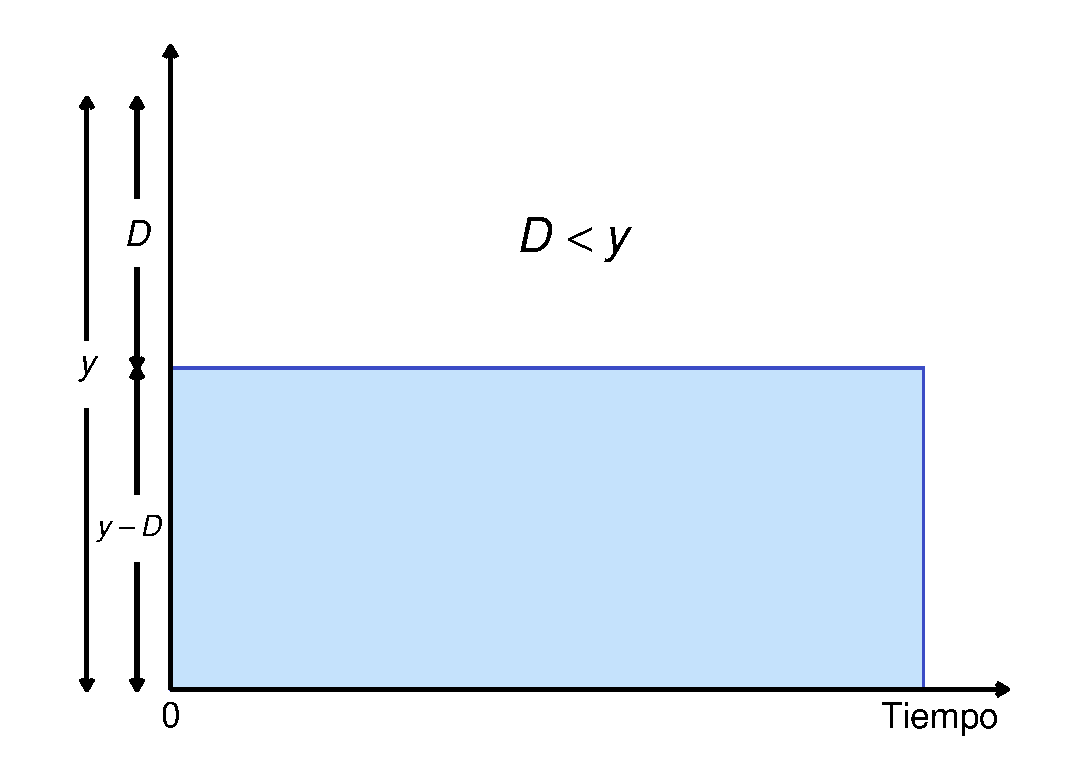
\includegraphics[width=0.48\textwidth,height=7cm]{images/img12.pdf}
        \label{fig:img12a}
    }
    \hfill
    \subfloat[(b)]{
        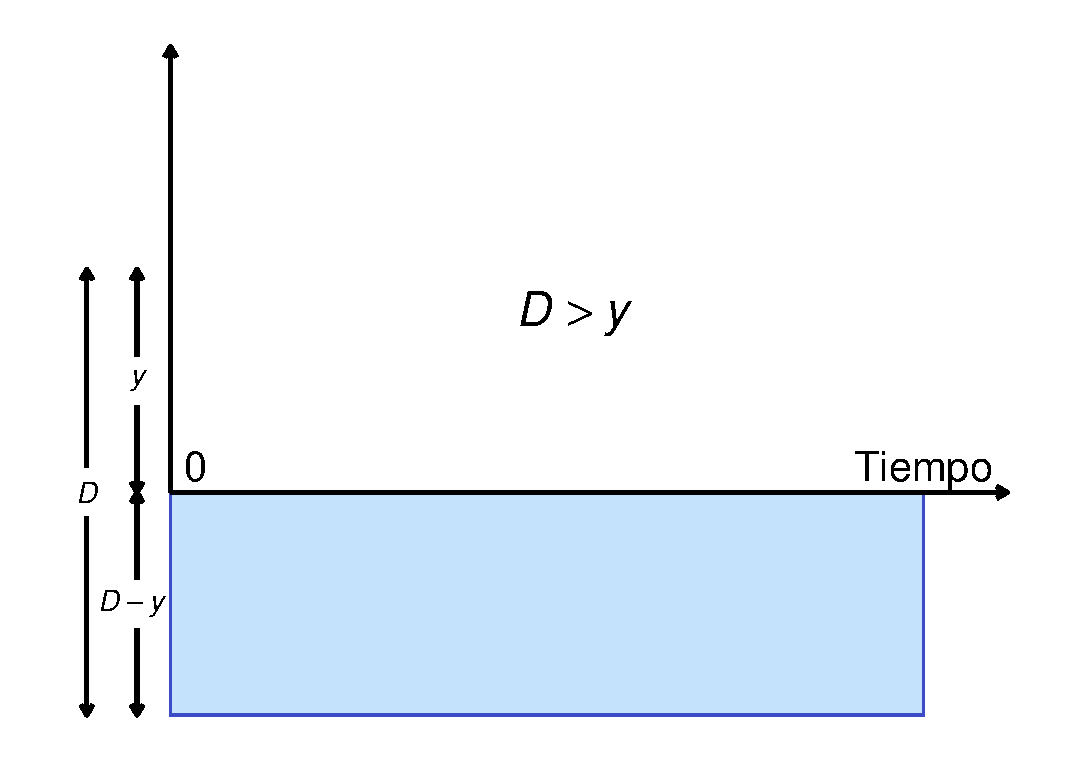
\includegraphics[width=0.48\textwidth,height=7cm]{images/img13.pdf}
        \label{fig:img12b}
    }

    \label{fig:img12}
\end{figure}

En el cual se tienen las siguientes suposiciones:
\begin{enumerate}
	\item En el momento que se recibe el pedido, la demanda empieza a ocurrir.
	\item No se tiene ningún costo de preparación. 
\end{enumerate}
De la Figura \ref{fig:img12} se tiene que si $D < y$, la cantidad sobrante $y-D$ se mantiene durante el periodo. Caso contrario si $D > y$ se tendrá una cantidad faltante $D-y$ durante el periodo.

Ahora el costo esperado durante el perido $E[C(y)]$ en función de la demanda estaría expresado para el caso discreto (\ref{VADiscreta}) y continuo (\ref{VAContinua}) teniendo las siguientes ecuaciones
\begin{eqnarray}
	\label{prob:un_periodo_con}
	E[C(y)] &=& h \int_{0}^{y} (y-D)f(D)dD + p \int_{y}^{\infty} (D-y)f(D)dD \quad \text{(caso continuo)} \\
	\label{prob:un_periodo_dis}
	E[C(y)] &=& h \sum\limits_{D = 0}^{y}(y-D)f(D) + p \sum\limits_{D = y+1}^{\infty} (D-y)f(D) \quad \text{(caso discreto)}
\end{eqnarray}
En lo cual se observa que $E[C(y)]$ en (\ref{prob:un_periodo_con}) y (\ref{prob:un_periodo_dis}) son convexos.

Para el caso continuo (\ref{prob:un_periodo_con}) como es convexo en ``$y$'' tiene un mínimo único. Tomando la primera derivada con respecto a ``$y$'' se tiene la siguiente expresión
\begin{eqnarray}
	\label{prob:der_E_con}
	\frac{d E[C(y)]}{dy} &=& \frac{d}{dy} \left[ h \int_{0}^{y} (y-D)f(D)dD + p \int_{y}^{\infty} (D-y)f(D)dD \right] \nonumber \\
	\frac{d E[C(y)]}{dy} &=& h \int_{0}^{y} f(D)dD - p \int_{0}^{\infty} f(D) dD
\end{eqnarray} 
Tomando en cuenta la segunda propiedad de la definición de variable aleatoria continua (\ref{VAContinua}), se puede realizar la siguiente expresión:
\begin{itemize}
 	\item $P[x \leq X] = \int_{0}^{X} f(x)dx$ 
 	\item $1 - P[x \leq X] = \int_{0}^{\infty} f(x)dx$
\end{itemize} 
Reemplazando en la expresión (\ref{prob:der_E_con}) se tiene la siguiente igualdad
\begin{eqnarray}
	\frac{d E[C(y)]}{dy} &=& hP[D \leq y] - p(1 - P[D \leq y]) \nonumber \\
	\frac{d E[C(y)]}{dy} &=& P[D \leq y] (h + p) - p \nonumber
\end{eqnarray}
E igualando a cero se tiene la siguiente igualdad:
\begin{eqnarray}
	\label{prob:P_D_men_y_opt}
	P[D \leq y] (h + p) - p &=& 0 \nonumber \\
	P[D \leq y^*] &=& \frac{p}{h+p}
\end{eqnarray}
Ahora para el caso discreto (\ref{prob:un_periodo_dis}) tomemos en cuenta las siguientes condiciones necesarias de optimalidad
\begin{itemize}
	\item $E[C(y-1)] \geq E[C(y)]$ y
	\item $E[C(y+1)] \geq E[C(y)]$ 
\end{itemize}
Que son suficientes ya que $E[C(y)]$ es una función convexa, empezemos hallando la expresiòn para $E[C(y+1)]$ en base a (\ref{prob:un_periodo_dis}) quedando de la siguiente manera
\begin{eqnarray}
	E[C(y+1)] &=& h \sum\limits_{D = 0}^{(y+1)}((y+1)-D)f(D) + p \sum\limits_{D = (y+1)+1}^{\infty} (D-(y+1))f(D) \nonumber \\
	E[C(y+1)] &=& h \left[ \sum\limits_{D = 0}^{y+1}(y+1)f(D) - \sum\limits_{D = 0}^{y+1}Df(D) \right] + \nonumber \\
	 & & p \left[ \sum\limits_{D = y+2}^{\infty} (D-y-1)f(D) \right] \nonumber \\
	E[C(y+1)] &=& h \left[ (y+1) \left( \sum\limits_{D = 0}^{y}f(D)+f(y+1) \right) - \left(\sum\limits_{D = 0}^{y} Df(D) + (y+1)f(y+1) \right) \right] + \nonumber \\
	 & & p \left[ \sum\limits_{D = y+1}^{\infty}(D-y-1)f(D)-( (y+1)-y-1 )f(y+1) \right] \nonumber \\
	 E[C(y+1)] &=& h \left[ (y+1) \sum\limits_{D = 0}^{y} f(D) + (y+1)f(y+1) - \sum\limits_{D = 0}^{y} Df(D) - (y+1)f(y+1) \right] + \nonumber \\
	  & & p \left[ \sum\limits_{D = y+1}^{\infty} (D-y-1)f(D) \right] \nonumber \\
	 E[C(y+1)] &=& h \left[ (y+1) \sum\limits_{D = 0}^{y} f(D) - \sum\limits_{D = 0}^{y} Df(D) \right] + \nonumber \\
	  & & p \left[ \sum\limits_{D = y+1}^{\infty} (D-y-1)f(D) \right] \nonumber \\
	E[C(y+1)] &=& h \left[ \sum\limits_{D = 0}^{y} (y+1-D) f(D) \right] + \nonumber \\
	  & & p \left[ \sum\limits_{D = y+1}^{\infty} (D-y-1)f(D) \right] \nonumber \\
	E[C(y+1)] &=& h \sum\limits_{D = 0}^{y}(y-D)f(D) + h \sum\limits_{D = 0}^{y}f(D) + p \sum\limits_{D = y+1}^{\infty}(D-y)f(D) - p \sum\limits_{D = y+1}^{\infty} f(D) \nonumber
\end{eqnarray}
\begin{eqnarray}
	\label{seguimos_res}
	E[C(y+1)] &=& h \sum\limits_{D = 0}^{y} (y-D) f(D) + p \sum\limits_{D = y+1}^{\infty} (D-y)f(D) + h \sum\limits_{D = 0}^{y} f(D) - p \sum\limits_{D = y+1}^{\infty} f(D) \nonumber \\
	E[C(y+1)] &=& E[C(y)] + h \sum\limits_{D = 0}^{y} f(D) - p \sum\limits_{D = y+1}^{\infty} f(D)
\end{eqnarray}
Por la segunda satisfacción de la definición (\ref{defn_vadisc}) de variable aleatoria discreta (\ref{VADiscreta}) se tiene la siguiente igualdad:
\begin{eqnarray}
	\sum\limits_{D = 0}^{y}f(D) + \sum\limits_{D = y+1}^{\infty} f(D) &=& 1 \nonumber \\
	\sum\limits_{D = y+1}^{\infty} f(D) &=& 1 - \sum\limits_{D = 0}^{y}f(D) \nonumber
\end{eqnarray}
Reemplazando esta igualdad en la expresión (\ref{seguimos_res}) obtenemos lo siguiente
\begin{eqnarray}
	\label{prob:Prim_cond_optima}
	E[C(y+1)] &=& E[C(y)] + h \sum\limits_{D = 0}^{y} f(D) - p \left(1 - \sum\limits_{D = 0}^{y}f(D) \right) \nonumber \\
	E[C(y+1)] - E[C(y)] &=& h \sum\limits_{D = 0}^{y} f(D) - p + p \sum\limits_{D = 0}^{y}f(D) \nonumber \\
	E[C(y+1)] - E[C(y)] &=& (h+p) \sum\limits_{D = 0}^{y}f(D)  - p \nonumber \\
	E[C(y+1)] - E[C(y)] &=& (h+p) P[D \leq y] - p
\end{eqnarray}
De la misma forma ahora hallando la expresiòn para $E[C(y-1)]$ en base a (\ref{prob:un_periodo_dis}) se tiene
\begin{eqnarray}
	E[C(y-1)] &=& h \sum\limits_{D = 0}^{(y-1)}((y-1)-D)f(D) + p \sum\limits_{D = (y-1)+1}^{\infty} (D-(y-1))f(D) \nonumber \\
	E[C(y-1)] &=& h \sum\limits_{D = 0}^{y-1}(y-D)f(D) - h \sum\limits_{D = 0}^{y-1}f(D) + p \sum\limits_{D = y}^{\infty} (D-y)f(D) + p \sum\limits_{D = y}^{\infty} f(D) \nonumber \\
	E[C(y-1)] &=& h \left[ \sum\limits_{D = 0}^{y}(y-D)f(D) - (y-y)f(y) \right] - h \sum\limits_{D = 0}^{y-1}f(D) \nonumber \\
	 & & + p \left[ \sum\limits_{D = y+1}^{\infty}(D-y)f(D) + (y-y)f(y) \right] + p \sum\limits_{D = y}^{\infty} f(D) \nonumber \\
	E[C(y-1)] &=& h \sum\limits_{D = 0}^{y}(y-D)f(D) - h \sum\limits_{D = 0}^{y-1}f(D) + p \sum\limits_{D = y+1}^{\infty} (D-y)f(D) + p \sum\limits_{D = y}^{\infty} f(D) \nonumber
\end{eqnarray}
\begin{eqnarray}
	\label{seguimos_res2}
	E[C(y-1)] &=& h \sum\limits_{D = 0}^{y}(y-D)f(D) + p \sum\limits_{D = y+1}^{\infty} (D-y)f(D) - h \sum\limits_{D = 0}^{y-1}f(D) + p \sum\limits_{D = y}^{\infty} f(D) \nonumber \\
	E[C(y-1)] &=& E[C(y)] - h \sum\limits_{D = 0}^{y-1}f(D) + p \sum\limits_{D = y}^{\infty} f(D)
\end{eqnarray}	
De la misma forma por la definición (\ref{defn_vadisc}) de variable aleatoria discreta (\ref{VADiscreta}) se tiene la siguiente igualdad:
\begin{eqnarray}
	\sum\limits_{D = 0}^{y-1}f(D) + \sum\limits_{D = y}^{\infty} f(D) &=& 1 \nonumber \\
	\sum\limits_{D = y}^{\infty} f(D) &=& 1 - \sum\limits_{D = 0}^{y-1}f(D) \nonumber
\end{eqnarray}
Reemplazando esta igualdad en la expresión (\ref{seguimos_res2}) obtenemos lo siguiente
\begin{eqnarray}
	\label{prob:Seg_cond_optima}
	E[C(y-1)] &=& E[C(y)] - h \sum\limits_{D = 0}^{y-1}f(D) + p \left( 1 - \sum\limits_{D = 0}^{y-1}f(D) \right) \nonumber \\
	E[C(y-1)] - E[C(y)] &=& - h \sum\limits_{D = 0}^{y-1}f(D) + p - p \sum\limits_{D = 0}^{y-1} f(D) \nonumber \\
	E[C(y-1)] - E[C(y)] &=& - (h+p) \sum\limits_{D = 0}^{y-1}f(D) + p \nonumber \\
	E[C(y-1)] - E[C(y)] &=& - (h+p) P[D \leq y-1] + p
\end{eqnarray}
En lo cual tomando la primera condición de optimalidad $E[C(y-1)] \geq E[C(y)]$ y reemplazando por los valores de (\ref{prob:Seg_cond_optima}) se tiene la siguiente desigualdad
\begin{eqnarray}
	\label{prob:seg_cond_des}
	E[C(y-1)] & \geq & E[C(y)] \nonumber \\
	E[C(y-1)] - E[C(y)] & \geq & 0 \nonumber \\
	- (h+p) P[D \leq y-1] + p & \geq & 0 \nonumber \\
	(h+p) P[D \leq y-1] - p & \leq & 0 \nonumber \\
	P[D \leq y-1] & \leq & \frac{p}{h+p}
\end{eqnarray}
Tomando la segunda condición de optimalidad $E[C(y+1)] \geq E[C(y)]$ y reemplazando por los valores de (\ref{prob:Prim_cond_optima}) se tiene la siguiente desigualdad
\begin{eqnarray}
	\label{prob:prim_cond_des}
	E[C(y+1)] & \geq & E[C(y)] \nonumber \\
	E[C(y+1)] - E[C(y)] & \geq & 0 \nonumber \\
	(h+s) P[D \leq y] - p & \geq & 0 \nonumber \\
	P[D \leq y] & \geq & \frac{p}{h+p}
\end{eqnarray}
Ahora tomando las expresiones (\ref{prob:seg_cond_des}) y (\ref{prob:prim_cond_des}) se tiene la siguiente desigualdad
\begin{equation}
	P[D \leq y^* - 1] \leq \frac{p}{h+p} \leq P[D \leq y^*]
\end{equation}

\manualsubsubsection{2.2.16.4}{Modelo de un periodo con costos de preparación}
Siendo igual que el modelo anterior de un periodo sin costos de preparación, en este modelo se incide el costo de preparación denotado por $K$. Entonces tomando en cuenta la expresión (\ref{prob:un_periodo_con}) y le adjuntamos el costo de preparación, se tiene la siguiente expresión para el costo esperado durante el periodo $E[\bar{C}(y)]$:
\begin{eqnarray}
	E[\bar{C}(y)] &=& K + E[C(y)] \nonumber \\
	E[\bar{C}(y)] &=& K + h \int_{0}^{y} (y-D)f(D)dD + p \int_{y}^{\infty} (D-y)f(D)dD
\end{eqnarray}
De la misma manera el valor óptimo $y^*$ de la expresión (\ref{prob:P_D_men_y_opt}) se debe satisfacer lo siguiente
\begin{equation}
	P[y \leq y^*] = \frac{p}{h+p}
\end{equation}
Tomando a $K$ como una constante el valor mínimo de $E[\bar{C}(y)]$ ocurre también en $y^*$. La política de pedido óptima se observa en la Figura \ref{fig:img14}.
\newpage
\begin{figure}[H]
  \caption{Política de pedido óptima (s-S) del modelo de un solo periodo con costo de preparación}
  {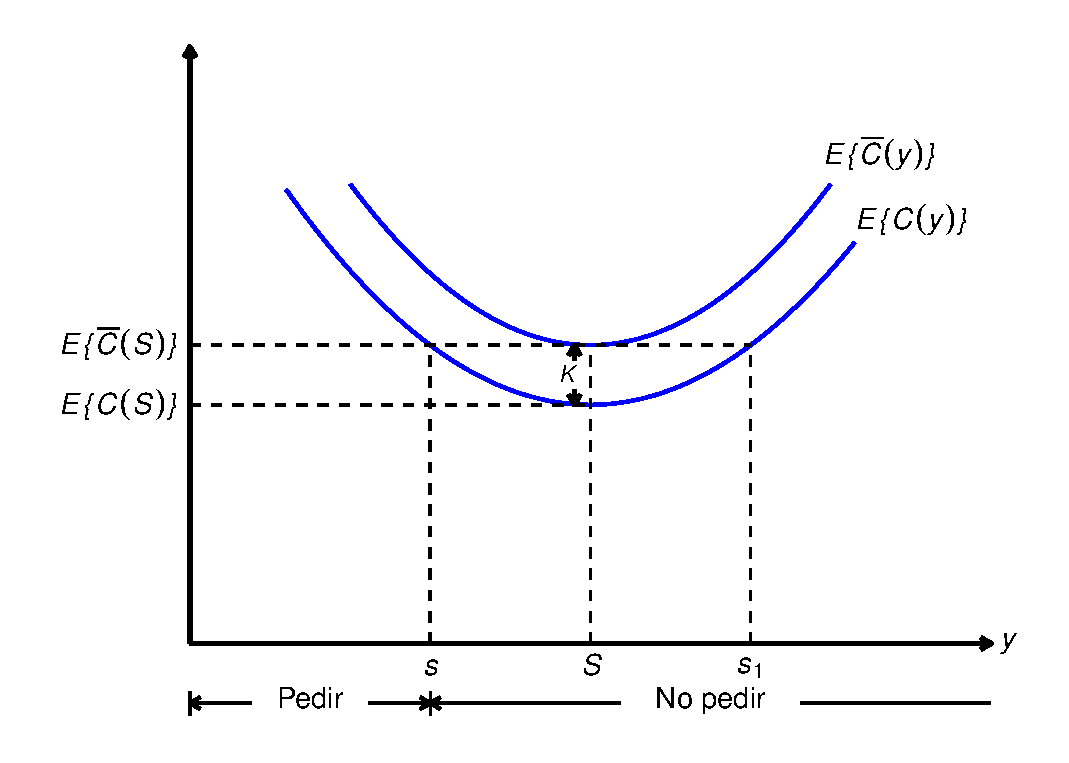
\includegraphics[width=13.5cm, height=7cm]{images/img14.pdf}}
  \label{fig:img14}
\end{figure}
En el cual se observa que si $S = y^*$ y el valor de $s < S$ se puede determinar mediante la siguiente ecuación:
\begin{eqnarray}
	E[C(s)] &=& E[\bar{C}(S)] \nonumber \\
	E[C(s)] &=& K + E[C(S)], \quad s < S
\end{eqnarray}
Si en la ecuación se tiene otro valor ${s}_{1} > S$ se le descarta. 

Entonces para la política de pedido suponemos que $x$ es la cantidad disponible antes de colocar el siguiente pedido, se tienen tres condiciones:
\begin{enumerate}
	\item $x < s$
	\item $s \leq x \leq S$
	\item $x > S$ 
\end{enumerate}

\begin{description}
    \item[\textbf{Caso 1 $(x > s)$:}] Como ya se tiene una cantidad $x$ en el cual su costo equivale a $E[C(x)]$. Si realizamos un pedido adicional $y-x$ donde $y > x$ su costo para $y$ estaría dado por $E[\bar{C}(y)]$ en el que se incluye el costo de preparación $K$. De la Figura \ref{fig:img14} se tiene
    $$
        \min_{y>x} E[\bar{C}(y)] = E[\bar{C}(S)] < E[C(x)]
    $$
    En el que la política de inventario óptima es pedir $S-x$ unidades.

    \item[\textbf{Caso 2 $(s \leq x \leq S)$:}] De la Figura \ref{fig:img14} se tiene
    $$
        E[C(x)] \leq \min_{y>x}E[\bar{C}(y)] = E[\bar{C}(S)]
    $$
    En el que la política de inventario indica que no se debería realizar el pedido para este caso. Por lo que $y^* = x$.

    \item[\textbf{Caso 3 $(x > S)$:}] De la Figura \ref{fig:img14} se tiene que $y > x$
    $$
        E[C(x)] < E[\bar{C}(y)]
    $$
    Al igual que en el caso 2, no se debería realizar el pedido o sea $y^* = x$.
\end{description}

Por lo que la política de inventario utiliza la \textsl{política s-S} que resume el pedido de la siguiente manera

\begin{equation}
	y^* =
	\left\{
	\begin{array}{ll}
		S-x & \text{si } x < s \\
		x, & \text{si } x \geq s
	\end{array}
	\right.
\end{equation}
En el cual se debe realizar el pedido $(S-x)$ si $x < s$ y no realizar el pedido si $x \geq s$, esta política esta garantizado ya que la función de costo es convexa.

\manualsubsubsection{2.2.16.5}{Modelo de varios periodos}
A diferencia de los dos anteriores modelos mencionados, en este modelo se presentan varios periodos bajo el supuesto de que no se tenga costo de preparación. Además se permite un retraso en el cumplimiento de la demanda y no se tiene un retraso en la entrega.

La demanda $D$ sigue una función de densidad $f(D)$ para cualquier periodo. Se tiene un factor de descuento $\alpha$ tal que $\alpha < 1$, por lo que la cantidad monetario disponible $A$ durante los $n$ periodos tendrán un valor de ${\alpha}^{n}A$. En el caso de que el inventario tenga $n$ periodos y que la escasez se deja pendiente en un periodo se define
\begin{itemize}
	\item[${F}_{i}({x}_{i}) =$] Utilidad máxima esperada durante los periodos $i, i+1, i+2, \cdots, n$ dado que ${x}_{i}$ es la cantidad disponible antes de colocar el siguiente pedido en el periodo $i$  
\end{itemize}
Teniendo en cuenta el costo e ingreso por unidad denotadas por $c$ y $r$ respectivamente, asimismo tomando las notaciones vistas en los modelos de un periodo y ${F}_{n+1}({y}_{n}-D)=0$ se tiene el siguiente modelo de programación probabilística.
\begin{align}
    F_{i}(x_{i}) &= \max_{y_{i} \geq x_{i}} 
    \left\{ -c({y}_{i}-{x}_{i}) + \int_{0}^{{y}_{i}} \left[ rD - h ({y}_{i}-D) \right] f(D) dD \right. \nonumber \\
    & \quad + \int_{{y}_{i}}^{\infty} \left[ r{y}_{i}+ \alpha r (D-{y}_{i}) - p(D-{y}_{i}) \right] f(D) dD \nonumber \\
    & \quad + \alpha \int_{0}^{\infty} F_{i+1}({y}_{i}-D) f(D) dD 
    \left. \vphantom{\int_{0}^{\infty}} \right\}, \quad \text{para } i = 1,2, \dots, n
\end{align}

El valor de ${x}_{i}$ puede ser negativa por la escasez pendiente, se incluye la cantidad $\alpha r (D-{y}_{i})$ en la segunda integral porque $(D - {y}_{i})$ es la demanda no satisfecha en el periodo $i$ que debe ser satisfecha en el periodo $i+1$. El problema se resuelve mediante la manera recursiva. Si la cantidad de pedidos en los periodos es finita, la ecuación recursiva se reduce a
\begin{align}
    F(x) &= \max_{y \geq x} 
    \left\{ -c(y-x) + \int_{0}^{y} \left[ rD - h (y-D) \right] f(D) dD \right. \nonumber \\
    & \quad + \int_{y}^{\infty} \left[ ry+ \alpha r (D-y) - p(D-y) \right] f(D) dD \nonumber \\
    & \quad + \alpha \int_{0}^{\infty} F(y-D) f(D) dD 
    \left. \vphantom{\int_{0}^{\infty}} \right\}
\end{align}
Donde ``$x$'' y ``$y$'' son los inventarios durante cada periodo antes y después de recibir el pedido respectivamente.

El valor óptimo de $y$ se determina a partir de la siguiente condición necesaria y suficiente ya que la función de ingreso $F(x)$ es cóncava
\newpage
\begin{align}
	\label{prob:alpha_der_partial}
    \frac{\partial F(x)}{\partial y}  &= \frac{\partial}{\partial y} 
    \left[ \max_{y \geq x} \left\{ -c(y-x) + \int_{0}^{y} \left[ rD - h (y-D) \right] f(D) dD \right. \right. \nonumber \\
    & \quad + \int_{y}^{\infty} \left[ ry+ \alpha r (D-y) - p(D-y) \right] f(D) dD \nonumber \\
    & \quad + \alpha \int_{0}^{\infty} F(y-D) f(D) dD 
    \left. \vphantom{\int_{0}^{\infty}} \right\} 
    \left. \vphantom{\int_{0}^{\infty}} \right] \nonumber \\
    \frac{\partial F(x)}{\partial y}  &= -c -h \int_{0}^{y}f(D)dD + \int_{y}^{\infty}[(1- \alpha )r + p]f(D)dD \nonumber \\
    & \quad + \alpha \int_{0}^{\infty} \frac{\partial F(y-D)}{\partial y}f(D)dD = 0
\end{align}

El valor de $\frac{\partial F(y-D)}{\partial y}$ se determina de la siguiente manera. Si hay más unidades $\beta > 0$ disponibles al inicio del siguiente periodo, la utilidad del siguiente periodo se incrementará en $c \beta$, ya que se pide esa cantidad de manera menor, lo que indica que:
$$
\frac{\partial F(y-D)}{\partial y}=c
$$
De lo que en (\ref{prob:alpha_der_partial}) la condición necesaria es
$$
-c-h \int_{0}^{y}f(D)dD+[(1-\alpha)r+p]\left( 1- \int_{0}^{y}f(D)dD \right) + \alpha c \int_{0}^{\infty}f(D)dD = 0
$$
Sea $w = \int_{0}^{y}f(D)dD$ y además se sabe que $\int_{0}^{\infty}f(D)dD=1$ por la definición de variable aleatoria continua ($\ref{VAContinua}$), reemplazando en la condición y resolviendo se tiene la siguiente expresión
\begin{eqnarray}
	-c-hw+[(1-\alpha)r+p](1-w)+\alpha c &=& 0 \nonumber \\
	-c-hw+[r-\alpha r + p](1-w)+ \alpha c &=& 0 \nonumber \\
	-c-wh+r-\alpha r + p - wr + w \alpha r - w p + \alpha c &=& 0 \nonumber \\
	wh + wr - w \alpha r + wp &=& -c+r - \alpha r + p + \alpha c \nonumber \\
	w (h+r- \alpha r + p) &=& p + r - \alpha r - c + \alpha c \nonumber \\
	w (p+h+r- \alpha r) &=& p + r(1 - \alpha) -c(1 - \alpha) \nonumber
\end{eqnarray}
\begin{eqnarray}
	w (p+h+r(1- \alpha)) &=& p + (r-c)(1 - \alpha) \nonumber \\
	w &=& \frac{p + (r-c)(1 - \alpha)}{p+h+r(1- \alpha)} \nonumber
\end{eqnarray}
Reemplazando $w = \int_{0}^{y}f(D)dD$ se tiene el nivel óptimo del inventario $y^*$ determinado a partir de
\begin{equation}
	\int_{0}^{y^*}f(D)dD = \frac{p + (r-c)(1 - \alpha)}{p+h+r(1- \alpha)}
\end{equation}
En el cual la política de inventario óptima durante cada periodo, si el nivel de inventario es $x$ se da de la siguiente manera
\begin{equation}
	y^* =
	\left\{
	\begin{array}{ll}
		y^* - x & \text{si } x < y^* \\
		x, & \text{si } x \geq y^*
	\end{array}
	\right.
\end{equation}
En el cual se debe realizar el pedido $({y}^{*}-x)$ si $x < y^*$ y no realizar el pedido si $x \geq y^*$.
%--------------------------------------------
%----------- ORGANIZACION DEL CSI   ---------
%--------------------------------------------
%\newpage
\subsection{Organización del centro de salud integral ``La Fuente''}

\subsubsection{Historia}
\textsl{LA FUENTE CENTRO DE SALUD INTEGRAL} es una Organización Cristiana que opera desde el año 2005 en el distrito de San Jerónimo, Cusco, Perú. Se constituye formalmente como Asociación Civil Sin Fines de Lucro el 28 de Octubre del año 2008.

Nuestro deseo es brindar atención excelente en servicios de salud a la población del Cusco y su alrededor, y, al hacerlo, compartir el amor que Dios nos ha mostrado a través de Jesucristo.

Nuestro equipo esta compuesto por médicos norteamericanos titulados en su especialidad respectiva, y profesionales peruanos debidamente licenciados. Hablamos inglés, castellano y quechua.

\subsubsection{Misión}
Promover vidas saludables para nuestros pacientes, brindándoles la mejor atención a nuestro alcance: preventiva de rehabilitación y curativa, de manera integral, atendiendo tanto su salud física como espiritual, sobre el fundamento de nuestra fe en Jesucristo.

\subsubsection{Visión}
Ser, al 2035 una organización lider en salud a nivel nacional, y referente en Oftalmología a nivel global, que muestre a Jesucristo en cada servicio que brindamos a todas las personas que lleguen a nosotros.

\subsubsection{Valores}

\begin{table}[H]
    \caption{Valores La Fuente Centro de Salud Integral}
    \begin{tabular}{p{2.65cm} p{5.5cm} p{6cm} } % Define anchos personalizados para cada columna
        \hline
        \textbf{VALORES CENTRALES} & \textbf{METAS} & \textbf{PRINCIPIOS} \\
        \hline
        \textbf{Compasión} & Atención con empatía & Amor y cuidado \\
        \hline
        \textbf{Justicia} & Acceso equitativo & Equidad / No discriminación \\
        \hline
        \textbf{Servicio} & Servicios de alta calidad & Diligencia \\
        \hline
        \textbf{Integridad} & Promoción de las mejores prácticas éticas y transparentes & Alineación con valores cristianos \\
        \hline
        \textbf{Cooperación} & Trabajo efectivo en equipo & Impacto mediante la colaboración \\
        \hline
    \end{tabular}
\end{table}

\subsubsection{Estructura organizativa}

\begin{enumerate}
	\item \textbf{ORGANO DE DIRECCIÓN}
	\begin{enumerate}
		\item Dirección General
	\end{enumerate}
	\item \textbf{ORGANOS DE ASESORAMIENTO}
	\begin{enumerate}
		\item Departamento Legal
		\item Departamento de Contabilidad y Finanzas
		\item Medicina Ocupacional
		\item Seguridad y Salud en el Trabajo
		\item INLASER (Marketing) 
	\end{enumerate}
	\item \textbf{ORGANOS DE APOYO}
	\begin{enumerate}
		\item Administración General
		\item Dirección de Operaciones
		\item Departamento de Logística de Insumos Médicos
		\begin{itemize}
			\item Cotizaciones
			\item Almacén 
		\end{itemize}
		\item Ingeniería Biomédica
		\item Infraestructura y Servicios Generales
		\begin{itemize}
			\item Portería y Seguridad
			\item Limpieza y mantenimiento 
		\end{itemize}
		\item Sistemas $\&$ TI
		\begin{itemize}
			\item Soporte Técnico
			\item Software y Programación 
		\end{itemize}
		\item Gestión de HHCC
	\end{enumerate}
	\item \textbf{ORGANOS EN LINEA}
	\begin{enumerate}
	 	\item UPSS Farmacia
	 	\item Departamento de Fisioterapia
	 	\begin{itemize}
	 		\item Admisión / Recepción
	 		\item Consultorios Externos 
	 	\end{itemize}
	 	\item Departamento de Odontología
	 	\begin{itemize}
	 		\item Admisión / Recepción
	 		\item Consultorios Externos 
	 	\end{itemize}
	 	\item Departamento de Oftalmología
	 	\begin{itemize}
	 		\item Área de Admisión
	 		\begin{itemize}
	 		 	\item Admisión
	 		 	\item Recepción
	 		 \end{itemize}
	 		 \item Área de Asistencia Técnica
	 		 \begin{itemize}
	 		  	\item Triaje
	 		  	\item Indicaciones
	 		  	\item Exámenes Especiales 
	 		  \end{itemize}
	 		  \item Optometría
	 		  \item Oftalmología
	 		  \item Especialidades
	 		  \begin{itemize}
	 		   	\item Retina
	 		   	\item Glaucoma
	 		   	\item Oculoplastía 
	 		   \end{itemize}
	 		  \item Sala de Cirugías y Procedimientos
	 		  \begin{itemize}
	 		   	\item Cotizaciones
	 		   	\item Esterilización
	 		   	\item Cirugías no electivas y Electivas 
	 		   \end{itemize}
	 		  \item Óptica
	 		  \begin{itemize}
	 		   	\item Asesoría de Ventas
	 		   	\item Laboratorio Óptico 
	 		   \end{itemize} 
	 	\end{itemize}
	 \end{enumerate} 
\end{enumerate}

\begin{landscape} % Iniciar la página en formato horizontal
\begin{figure}[h!]
  \caption{Organigrama La Fuente Centro de Salud Integral}
  {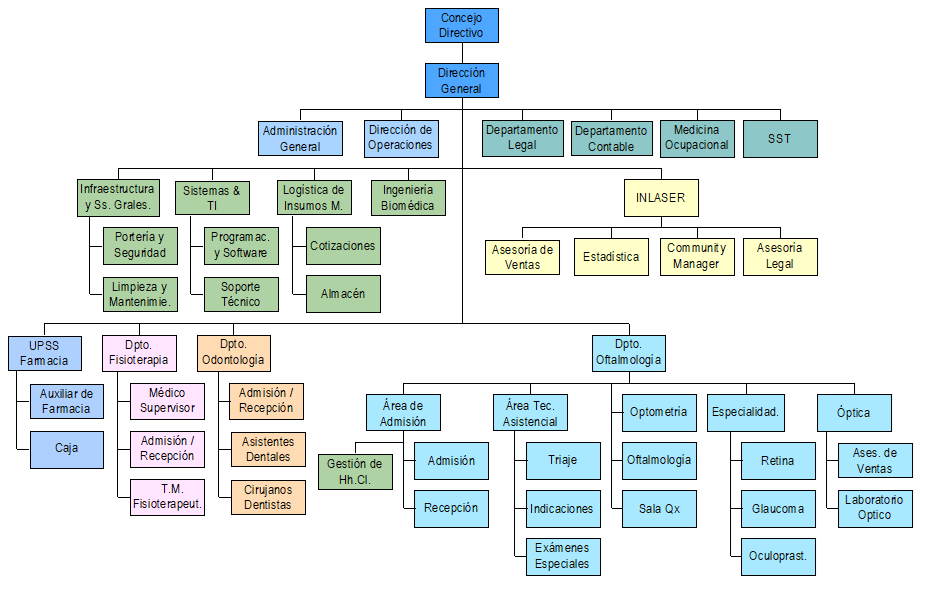
\includegraphics[width=25cm, height=14cm]{images/organigrama.png}}
  \label{fig:organigrama_fuente}
\end{figure} 
\end{landscape} % Finalizar la página horizontal

\section{Marco conceptual}
\noindent
\textbf{Análisis ABC:} Análisis que divide el inventario en tres grupos. El grupo A es más importante que el grupo B que, a su vez más importante que el C. \citep{render2006metodos}\vspace{0.25cm}

\noindent
\textbf{Inventario:} Es cualquier recurso almacenado que se utiliza para satisfacer una necesidad actual o futura. \citep{render2006metodos}\vspace{0.25cm}

\noindent
\textbf{Demanda:} Es la cantidad que los compradores desean adquirir o comprar de un determinado bien para satisfacer sus necesidades. \citep{mankiw2007principios}\vspace{0.25cm}

\noindent
\textbf{Costos:} Valor de mercado de los insumos que la empresa utiliza en la producción o mantenimiento del bien. Todo lo que el vendedor renuncia para producir el bien \citep{mankiw2007principios}\vspace{0.25cm}

\noindent
\textbf{Descuentos por cantidad:} Costo por unidad cuando se tienen grandes órdenes de un artículo. \citep{render2006metodos}\vspace{0.25cm}

\noindent
\textbf{Faltantes:} Situación que ocurre cuando no hay inventario en disponibilidad. \citep{render2006metodos}\vspace{0.25cm}

\noindent
\textbf{Punto de Reorden:} Momento en el que se toma la decisión de cuando realizar el pedido. \citep{taha2012investigacion}\vspace{0.25cm}

\noindent
\textbf{Tiempo de entrega:} Tiempo que se demora en recibir la orden una vez realizada. \citep{render2006metodos}






















 
% Capitulo 4 - Metodologia
\newpage
\chapter{HIPÓTESIS Y VARIABLES}
\section{Hipótesis}

\section{Hipótesis general}
El control de almacén del centro de salud integral La Fuente del Cusco se optimizará mediante la aplicación de los modelos de inventarios.

\section{Hipótesis específicas}

\begin{itemize}
\item Los productos más demandados y/o costosos en el centro de salud integral La Fuente del Cusco vienen a ser aquellos usados en el área de oftalmología.
\item Los modelos de inventarios determinísticos se adecuan a los productos más demandados y/o costosos.
\item Las cantidades, tiempo y costos de inventarios se optimizarán aplicando los modelos de inventarios.
\item El aplicativo web de Shiny monitoreara y dara seguimiento a los productos del centro de salud integral La Fuente del Cusco.
\end{itemize}

\section{Identificación de variables e indicadores}
\subsection{Variables dependientes}
Las variables dependientes vienen a ser las respuestas a la política de inventarios sobre cuánto pedir y cuándo pedir expresados por el tiempo ($T^*$), la cantidad de pedidos ($y^*$), punto de reorden ($R$) y costos totales de inventarios $CTI(y^*)$ óptimos que van a estar influenciados principalmente por el comportamiento de la demanda y costos del inventario.
\clearpage
\subsection{Variables independientes}
\begin{itemize}
	\item Comportamiento de la demanda de los productos.
	\begin{itemize}
		\item Tiempos en reabastecer el pedido $(L)$
		\item Función de la demanda de los productos $(D)$ 
	\end{itemize}
	\item Costos de inventario
	\begin{itemize}
		\item Costo de compra $(C)$
		\item Costo de preparación $(K)$
		\item Costo de retención $(h)$
		\item Costo por escasez $(p)$
	\end{itemize}
	
\end{itemize}

\begin{landscape} % Iniciar la página en formato horizontal
\section{Operacionalización de variables}

\begin{longtable}{p{3.5cm}p{6.5cm}p{5cm}p{3cm}p{2.5cm}}
    \caption{Matriz de operacionalización de variables} 
    \label{tab:matriz_operacionalizacion} \\

    \hline
    \textbf{Variable} & \textbf{Definición} & \textbf{Indicador} & \textbf{Tipo} & \textbf{Escala} \\
    \hline
    \endfirsthead

    \hline
    \textbf{Variable} & \textbf{Definición} & \textbf{Indicador} & \textbf{Tipo} & \textbf{Escala} \\
    \hline
    \multicolumn{5}{l}{\textbf{Independiente}} \\ % Se repite al inicio de cada nueva página
    \hline
    \endhead

    \hline
    \endfoot

    \hline
    \endlastfoot

    \multicolumn{5}{l}{\textbf{Dependiente}} \\
    \hline
    Cantidad de pedido óptimo & Es la cantidad de pedido óptimo que tiene la política del producto, que responde a ¿Cuánto pedir? \citep{taha2012investigacion} & Cantidad o unidades del producto que se deben realizar $(y^*)$ & Continua & Razón \\
    \hline
    Tiempo de pedido óptimo & Es el tiempo de pedido óptimo que tiene la política del producto, que responde a ¿Cuándo pedir? \citep{taha2012investigacion} & Tiempo de solicitud del producto $(T^*)$ & Discreta & Razón \\
    \hline
    Punto de reorden & Es la cantidad del producto que debe llegar para realizar el siguiente pedido. \citep{taha2012investigacion} & Cantidad del producto para realizar el siguiente pedido ($R$) & Continua & Razón \\
    \hline
    Costo total del inventario óptimo & Es el costo total que se tendrá aplicando la política de inventarios. \citep{taha2012investigacion} & Costo total de inventario $CTI(y^*)$ & Continua & Razón \\
    \hline
    Tiempo de reabastecimiento & Tiempo de entrega del proveedor desde que se realiza el pedido hasta el momento de la entrega. \citep{taha2012investigacion} & Tiempo desde la realización del pedido hasta la entrega ($L$) & Discreta & Razón \\
    \hline
    Demanda & Comportamiento del producto sobre sus salidas que se encuentra en base a las solicitudes realizadas por los usuarios que requieran dicho producto. \citep{hillier2003introduccion} & Demanda del producto ($D$) & Continua & Razón \\
    \hline
    \multirow{4}{*}{Costos} & \multirow{4}{6.5cm}{Es el monto que cuesta el producto en el inventario que se encuentra en función de los costos que conlleva poseer dicho producto. \citep{taha2012investigacion}} & Costo de compra ($C$) & Continua & Razón \\
    \cline{3-5}
    & & Costo de preparación ($K$) & Continua & Razón \\
    \cline{3-5}
    & & Costo de retención ($h$) & Continua & Razón \\
    \cline{3-5}
    & & Costo de escasez ($p$) & Continua & Razón \\
    \hline
\end{longtable}

\end{landscape} % Finalizar la página horizontal




















 
% Capitulo 4 - Metodologia
\newpage
\chapter{METODOLOGÍA}

\section{Ámbito de estudio: localización política y geográfica}

\section{Tipo y nivel de investigación}
El tipo de investigación es aplicada, como indican \cite{hernandez2020metodologia} se está evaluando los productos adquiridos para el funcionamiento del centro de salud integral, desde la selección de productos importantes que requieran un análisis más exhaustivo, los factores que influyen sobre el tiempo de pedido y las cantidades de pedido de esos productos, con la finalidad de encontrar una política óptima de inventarios. De esta forma aumentar el conocimiento científico sobre modelos de investigación operativa y resolver problemas de gestión y almacenamiento usando modelos de inventarios. 

\section{Unidad de análisis}
Esta investigación tiene enfoque cuantitativo dado que los datos recopilados tienen medición numérica en las características de los productos (entradas, salidas, espacio de almacenamiento, descuentos, entre otros) que serán utilizadas en las variables de estudio. De los cuáles serán analizados de forma descriptiva e inferencial según a los objetivos planteados. 

Además, para determinar la política óptima de inventario sobre cuánto pedir y cuándo pedir se utilizarán modelos matemáticos (modelos de inventarios determinísticos) y modelos estadísticos (modelos de inventarios probabilísticos) de inventarios que serán utilizados en el desarrollo de la investigación. \citep{hernandez2020metodologia}

\section{Población de estudio}
La población estará conformada por todos los productos que se encuentran en el almacén del centro de salud integral ``La Fuente'' del Cusco en el año 2024.

\section{Tamaño de muestra}
Para la investigación se obtuvo una cantidad total de 471 productos registrados en almacén del centro de salud integral. De la cual el único criterio de inclusión a tomar en cuenta para seleccionar los productos que se analizarán mediante los modelos de inventarios, seran aquellos que se encuentren en el grupo A de la clasificación de actividades basadas en costos (ABC), la justificación y uso de esta clasificación se detalla en el marco teórico del apartado (\ref{section:ABC})

\section{Técnicas de selección de muestra}
La técnica empleada es la revisión de documentos y/o análisis de datos secundarios del registro que se tienen de los productos de almacén del centro de salud integral.

\section{Técnicas de recolección de información}
Se consultaron los documentos como boletas, ordenes de compra, KARDEX, cotizaciones entre otros del departamento de logística el centro de salud integral ``La Fuente'' en el año 2024 con respecto a los datos específicos requeridos de los productos para el estudio.

\section{Técnicas de recolección de información}
Los datos serán recopilados y cargados en un archivo de extensión \textsl{.xlsx} para que posteriormente mediante el lenguaje de programación R y el entorno de desarrollo integrado RStudio se realice el análisis descriptivo apropiado asi como la clasificación ABC para seleccionar los productos que serán evaluados mediante el modelo de inventarios.

Seleccionando los productos en la categoría A se creará otro archivo de extensión \textsl{.xlsx} en donde se detallarán los movimientos recopilados en diferentes fechas del año 2024 de cada producto y se desarrollará la política de inventario según a los objetivos planteados en los cuales se describirá, analizará e interpretará los resultados obtenidos.

\section{Técnicas de análisis e interpretación de la información}

Las hipótesis de investigación planteadas en el estudio serán comprobadas mediante los resultados obtenidos por la política de inventarios, ya sea la clasificación ABC, los modelos de inventarios. De igual forma se utilizarán pruebas estadísticas para el caso de modelos inventarios estadísticos como la normalidad de datos.

\section{Técnicas para demostrar la verdad o falsedad de las hipótesis planteadas}

Las hipótesis de investigación planteadas en el estudio serán comprobadas mediante los resultados obtenidos por la política de inventarios, ya sea la clasificación ABC, los modelos de inventarios. De igual forma se utilizarán pruebas estadísticas para el caso de modelos inventarios estadísticos como la normalidad de datos.
% Capitulo 5 - Resultados
\newpage
\chapter{RESULTADOS}

Con el objetivo de determinar la política de inventario óptima, se tuvo un registro de los productos de almacén, donde primero se analizó los productos más demandados, seguidamente se extrajo el monto total en soles de cada producto que tuvo en el año 2024 así como el respectivo volumen de almacenamiento que tiene en $cm^3$. Para que sean evaluados descriptivamente mediante el análisis ABC y el diagrama de Pareto, seleccionando los productos que se analizarán mediante el modelo de inventarios.

\section{Análisis descriptivo de los productos de almacén}

Primeramente se describirá los 471 productos registrados mediante el área y la especialidad indicando su porcentaje en costos y almacenamiento.

\subsection{Nivel de área}

En esta parte se describirá los resultados en porcentaje de los costos y almacenamiento de los productos agrupados por áreas.

\begin{table}[H]
    \caption{Resultados por área de productos de almacén}
    \begin{tabular}{p{2cm} p{2.51cm} p{4cm} p{4cm}} % Define anchos personalizados para cada columna
        \hline
        \textbf{Área} & \textbf{Productos} & \textbf{$(\%)$ de Costos} & \textbf{$(\%)$ Ocupación} \\
        \hline
        \textbf{Oftalmología} & 212 & $92.86\%$ & $80.09\%$ \\
        \textbf{Odontología} & 259 & $7.14\%$ & $19.91\%$ \\
        \hline
        \textbf{Total} & 471 & $100\%$ & $100\%$
    \end{tabular}
    \label{table:Area_productos}
\end{table}

La Tabla \ref{table:Area_productos} describe los 471 productos de almacén agrupados por área, se muestra que la mayor parte de costos son productos del área de oftalmología con 212 productos tomando el $92.86\%$ de costos, seguido del área de odontología con 259 productos tomando el $7.14\%$ de costos. De la misma forma el porcentaje de ocupación de productos de oftalmología es del $80.09\%$ mientras que productos del área de odontología ocupan solo el $19.91\%$ del espacio de almacén.

\subsection{Nivel de especialidad}

Se describirá los resultados con respecto al porcentaje de costos y espacio de almacenamiento de los productos agrupados por especialidad.

\subsubsection{Área de oftalmología}

En almacén con respecto a insumos del área de oftalmología se tienen registrado 212 productos los cuales sirven para abastecer las diferentes especialidades y servicios que ofrece el centro de salud integral del área de oftalmología, de los cuales estos vienen a ser:

\begin{itemize}
    \item Insumos generales
    \item Tintas (usadas para las impresoras que se tienen)
    \item INLASER
    \item FACO
    \item Retina
    \item CROSSLINKING
    \item Esterilización
    \item Catarata
    \item ICL
    \item Glaucoma
    \item Oculoplastía
    \item Avastin 
\end{itemize}

\newpage

\begin{table}[H]
    \caption{Resultados de insumos del área de oftalmología por especialidad}
    \begin{tabular}{p{4cm} p{2.5cm} p{3cm} p{3cm}} % Define anchos personalizados para cada columna
        \hline
        \textbf{Especialidad} & \textbf{Productos} & \textbf{$(\%)$ de Costos} & \textbf{$(\%)$ Ocupación} \\
        \hline
        \textbf{INLASER} & 6 & $39.27\%$ & $2.20\%$ \\
        \textbf{FACO} & 6 & $25.49\%$ & $2.82\%$ \\
        \textbf{Insumos generales} & 105 & $9.95\%$ & $31.91\%$ \\
        \textbf{Tintas} & 27 & $5.62\%$ & $6.38\%$ \\
        \textbf{Esterilización} & 27 & $3.66\%$ & $27.32\%$ \\
        \textbf{CROSSLINKING} & 2 & $3.09\%$ & $0.48\%$ \\
        \textbf{Catarata} & 10 & $2.10\%$ & $1.96\%$ \\
        \textbf{Retina} & 16 & $1.94\%$ & $4.60\%$ \\
        \textbf{Glaucoma} & 3 & $0.68\%$ & $0.37\%$ \\
        \textbf{Oculoplastía} & 6 & $0.58\%$ & $0.48\%$ \\
        \textbf{ICL} & 2 & $0.28\%$ & $0.34\%$ \\
        \textbf{Avastín} & 2 & $0.19\%$ & $1.22\%$ \\
        \hline
        \textbf{Total} & 212 & $92.86\%$ & $80.09\%$
    \end{tabular}
    \label{table:productos_oftalmologia}
\end{table}

La Tabla \ref{table:productos_oftalmologia} describe los productos del área de oftalmología agrupados por especialidad en donde se muestra que la mayor cantidad de productos del área de oftalmología son insumos generales con 105 productos ocupando el $31.91\%$ de almacén, seguido de 27 productos de la especialidad de esterilización ocupando el $27.32\%$ de almacén, tintas con 27 productos ocupando el $6.38\%$ de almacén, retina con 16 productos ocupando el $4.60\%$ de almacén, FACO con 6 productos ocupando el $2.82\%$ de almacén, INLASER con 6 productos ocupando el $2.20\%$ de almacén, catarata con 10 productos ocupando el $1.96\%$ de almacén, avastin con 2 productos ocupando el $1.22\%$ de almacén, oculoplastía con 6 productos ocupando el $0.48\%$ de almacén, CROSSLINKING con 2 productos ocupando el $0.48\%$ de almacén, glaucoma con 3 productos ocupando el $0.37\%$ de almacén, y los productos que ocupan el menor espacio en almacén son de la especialidad de ICL con 2 productos ocupando solo el $0.34\%$

\newpage

\begin{figure}[h!]
  \caption{Productos del área de oftalmología por especialidad en base al ($\%$) de costos}
  {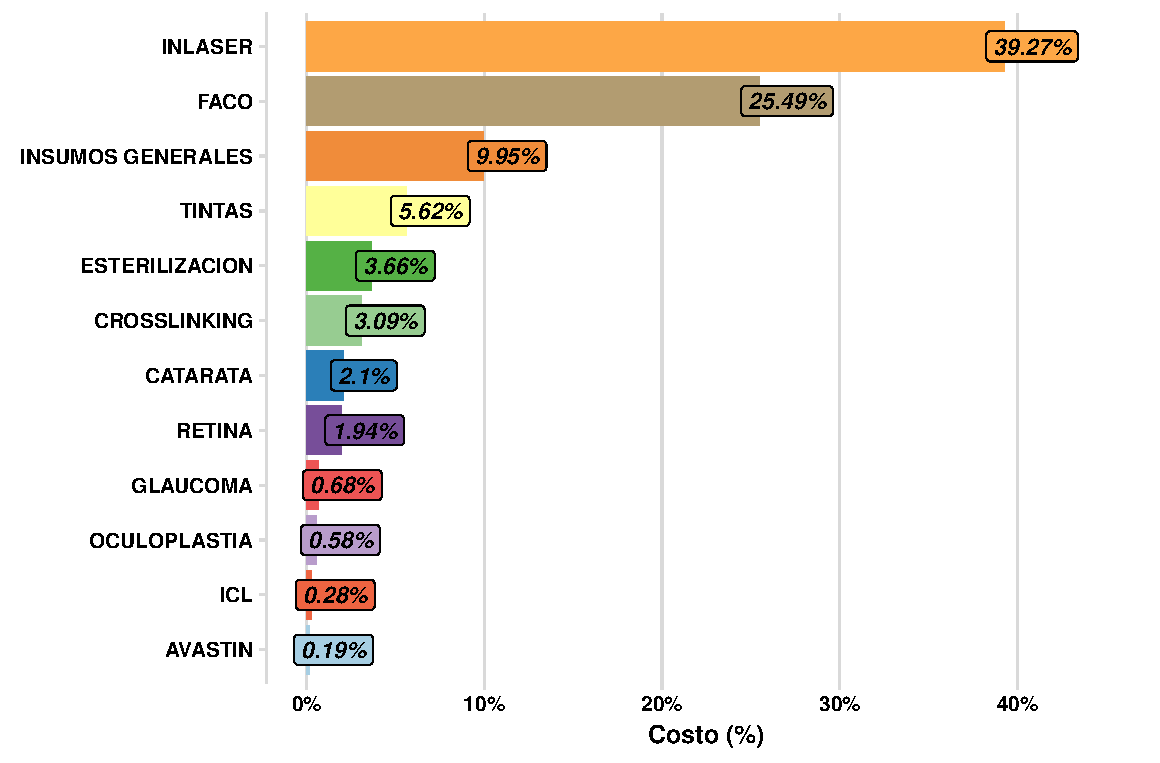
\includegraphics[width=15cm, height=10cm]{images/oftalm_prod.pdf}}
  \label{fig:Oftalm_espec}
\end{figure}

La Figura \ref{fig:Oftalm_espec} muestra un gráfico de barras de las especialidades del área de oftalmología ordenado por el porcentaje de costos, donde se observa que la mayor parte de los costos del área de oftalmología son de la especialidad de INLASER con el $39.27\%$ de los costos totales, seguido de la especialidad de FACO con el $25.49\%$ de costos, insumos generales con el $9.95\%$ de costos, tintas con el $5.62\%$ de costos, esterilización con el $3.66\%$ de costos, CROSSLINKING con $3.09\%$ de costos, catarata con $2.10\%$ de costos, retina con $1.94\%$ de costos, glaucoma con $0.68\%$ de costos, oculoplastía con $0.58\%$ de costos, ICL con $0.28\%$ de costos y de la especialidad de avastín con el $0.19\%$ de los costos totales.

\newpage

\subsubsection{Área de odontología}

En almacén con respecto a insumos del área de odontología se tienen registrado 260 productos los cuales sirven para abastecer las diferentes especialidades y servicios que ofrece el centro de salud integral en el área de odontología, de los cuales estos vienen a ser:

\begin{itemize}
    \item Prostodoncia
    \item Operatoria
    \item Endodoncia
    \item Cirugias
    \item Materiales
    \item Periodoncia
\end{itemize}

\begin{table}[H]
    \caption{Resultados de insumos del área de odontología por especialidad}
    \begin{tabular}{p{4cm} p{2.5cm} p{3cm} p{3cm}} % Define anchos personalizados para cada columna
        \hline
        \textbf{Especialidad} & \textbf{Productos} & \textbf{$(\%)$ de Costos} & \textbf{$(\%)$ Ocupación} \\
        \hline
        \textbf{Operatoria} & 93 & $2.09\%$ & $3.95\%$ \\
        \textbf{Prostodoncia} & 65 & $1.97\%$ & $4.24\%$ \\
        \textbf{Cirugías} & 16 & $1.28\%$ & $2.54\%$ \\
        \textbf{Materiales} & 25 & $0.92\%$ & $6.47\%$ \\
        \textbf{Endodoncia} & 51 & $0.68\%$ & $1.56\%$ \\
        \textbf{Periodoncia} & 9 & $0.19\%$ & $1.14\%$ \\
        \hline
        \textbf{Total} & 259 & $7.14\%$ & $19.91\%$
    \end{tabular}
    \label{table:productos_odontologia}
\end{table}

La Tabla \ref{table:productos_odontologia} describe los productos del área de odontología agrupados por especialidad, donde se muestra que la mayor cantidad de productos del área de odontología son materiales con 25 productos ocupando el $6.47\%$ de almacén, seguido de 65 productos de la especialidad de prostodoncia ocupando el $4.24\%$ de almacén, operatoria con 93 productos ocupando el $3.95\%$ de almacén, cirugías con 16 productos ocupando el $2.54\%$ de almacén, endodoncia con 51 productos ocupando el $1.56\%$ de almacén y periodoncia con 9 productos ocupando solo el $1.14\%$ de almacén.

\begin{figure}[H]
  \caption{Productos del área de odontología por especialidad en base al ($\%$) de costos}
  {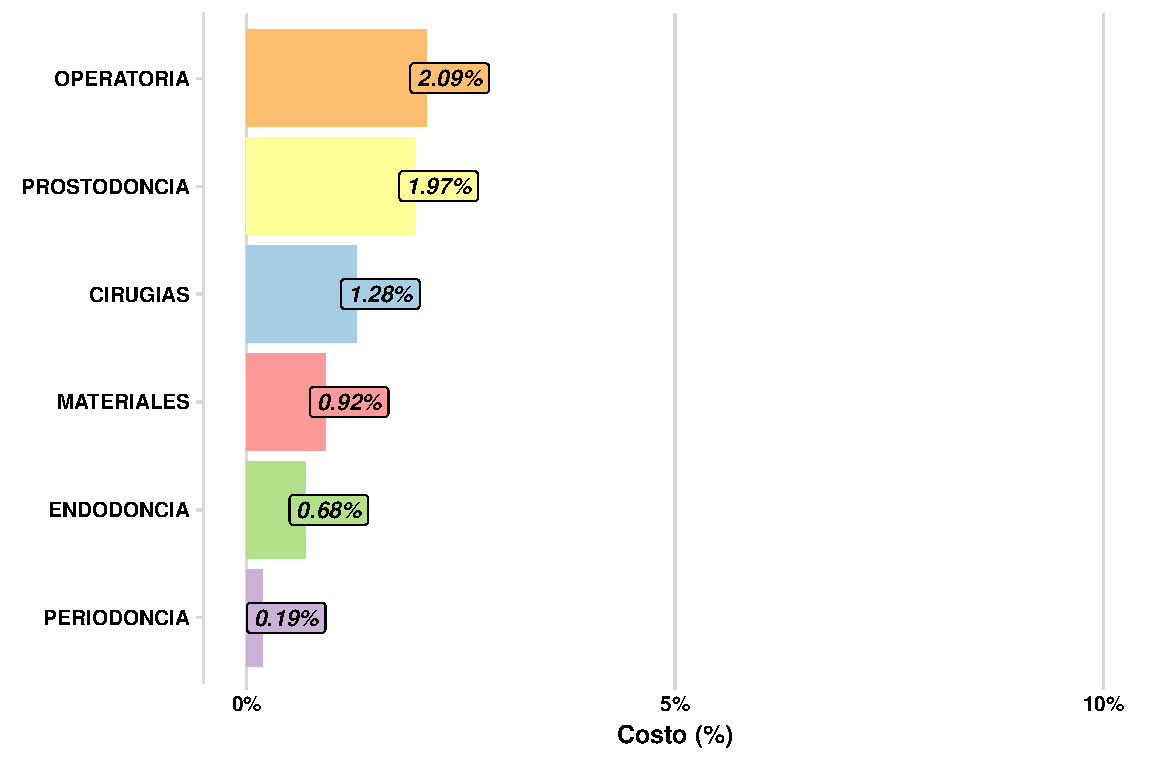
\includegraphics[width=15cm, height=10cm]{images/odonto_prod.pdf}}
  \label{fig:Odonto_espec}
\end{figure}

La Figura \ref{fig:Odonto_espec} muestra un gráfico de barras de las especialidades de odontología ordenados por el porcentaje de costos en donde se observa que la mayor parte de los costos del área de odontología son de la especialidad de operatoria con el $2.09\%$ de los costos totales, seguido de la especialidad de prostodoncia con el $1.97\%$ de costos, cirugías con $1.28\%$ de costos, materiales con $0.92\%$ de costos, endodoncia con $0.68\%$ de costos y de la especialidad de periodoncia con el $0.19\%$ de los costos totales.

\newpage

\section{Análisis descriptivo mediante actividades basadas en costos (ABC)}

Se describe la información de todos los productos registrados en función de los costos que vendrían a ser el costo total del año 2024 en salidas para evaluar la demanda en función monetaria, de la misma forma ver los espacios de almacenamiento. Este análisis será en función del porcentaje del total de costos y almacenamiento como se muestra en la Tabla \ref{table:ABC_resumen}

\begin{table}[H]
    \caption{Resultados de la clasificacìón (ABC)}
    \begin{tabular}{p{0.8cm} p{2.51cm} p{5.2cm} p{4.9cm}} % Define anchos personalizados para cada columna
        \hline
        \textbf{Grupo} & \textbf{Productos} & \textbf{$(\%)$ de Costos} & \textbf{$(\%)$ Ocupación} \\
        \hline
        \textbf{A} & 8 & $68.55\%$ & $3.74\%$ \\
        \textbf{B} & 34 & $21.36\%$ & $29.09\%$ \\
        \textbf{C} & 429 & $10.09\%$ & $67.17\%$ \\
        \hline
        \textbf{Total} & 471 & $100\%$ & $100\%$
    \end{tabular}
    \label{table:ABC_productos}
\end{table}

En la Tabla \ref{table:ABC_productos}, se muestra el análisis ABC de los productos de almacén del centro de salud clasificados mediante los costos producidos en el año 2024. De manera general se observa que la mayor denominación o cantidad de productos se encuentra en el grupo C con 429 productos ocupando el $67.17\%$ del espacio de almacén, seguido del grupo B con 34 productos ocupando el $29.09\%$ del espacio de almacén y por último el grupo A con 8 productos ocupando solo el $3.74\%$ del espacio de almacén.

\newpage
\begin{figure}[H]
  \caption{Diagrama de Pareto productos de almacén del centro de salud integral agrupados por análisis basados en costos (ABC)}
  {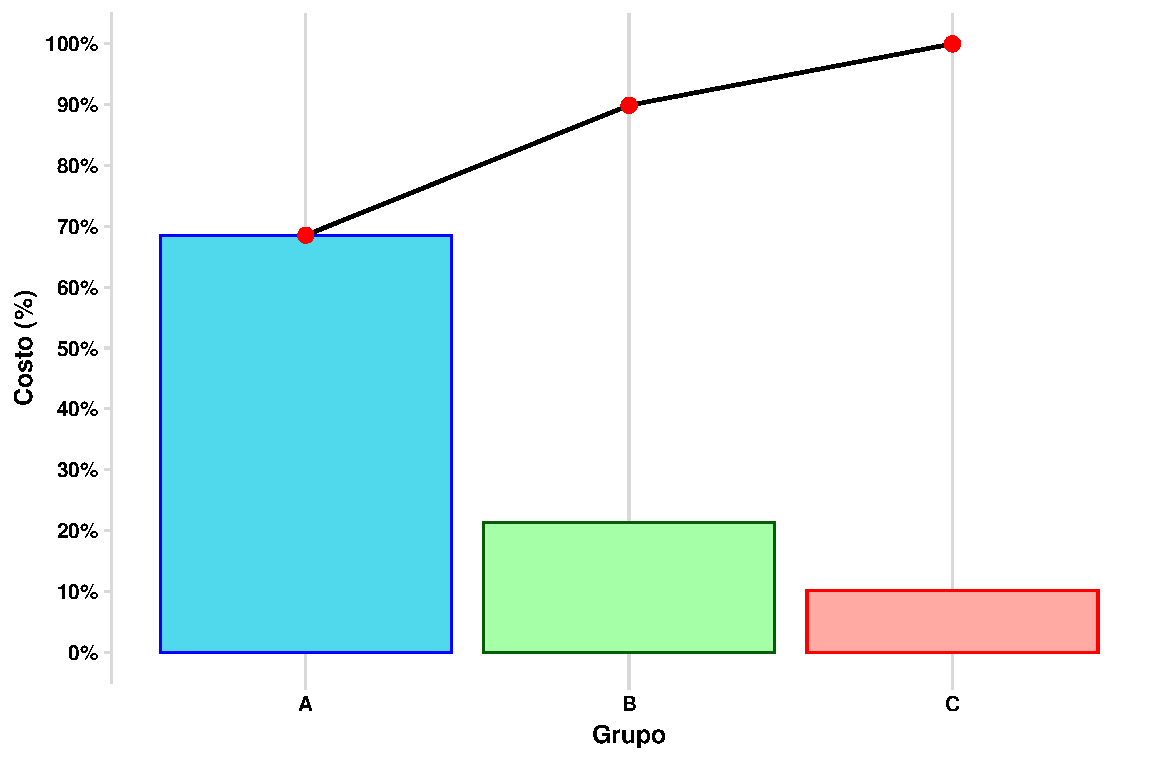
\includegraphics[width=15cm, height=7.9cm]{images/ABC.pdf}}
  \label{fig:ABC_almacen}
\end{figure}

En la Figura \ref{fig:ABC_almacen} se observa el diagrama de Pareto con respecto a los costos acumulados en el año 2024 de los productos de almacén del centro de salud integral, en donde se observa que los 8 productos del grupo A conforman un $68.55\%$ de los costos totales de almacén, los del grupo B el $21.36\%$ y los del grupo C solo el $10.09\%$ de costos totales.

\subsection{Selección de productos}

Tomando en cuenta los resultados de la Tabla \ref{table:ABC_productos} y el diagrama de Pareto de la Figura \ref{fig:ABC_almacen}, la política de inventarios debe priorizar a los 8 productos que se encuentran en el grupo A del análisis ABC. Siguiendo la metodología ABC de la sección (\ref{section:ABC}) se tomará los 8 productos del grupo A y productos del grupo B que tienen mayores costos, esto con la solicitud del área de logística del centro de salud siendo 10 productos adicionales. Teniendo un total de 18 productos seleccionados en los que se aplicarán los modelos de inventarios.

\subsubsection{Resultados descriptivos de productos seleccionados}

Se describirá los resultados con respecto al porcentaje de costos y espacio de almacenamiento de los productos seleccionados para el modelo de inventarios.

\begin{table}[H]
    \caption{Resultados por área de productos seleccionados mediante el análisis ABC}
    \begin{tabular}{p{2cm} p{2.51cm} p{4cm} p{4cm}} % Define anchos personalizados para cada columna
        \hline
        \textbf{Área} & \textbf{Productos} & \textbf{$(\%)$ de Costos} & \textbf{$(\%)$ Ocupación} \\
        \hline
        \textbf{Oftalmología} & 18 & $79.31\%$ & $24.44\%$ \\
        \hline
    \end{tabular}
    \label{table:GrupoA_Area_Productos}
\end{table}

La Tabla \ref{table:GrupoA_Area_Productos} muestra los productos seleccionados mediante el análisis ABC agrupados por área, en el que todos los 18 productos seleccionados son del área de oftalmología ocupando el $79.31\%$ de costos y ocupan un $24.44\%$ del espacio de almacén.

\begin{table}[H]
    \caption{Resultados por especialidad de productos seleccionados mediante el análisis ABC}
    \begin{tabular}{p{2.5cm} p{3cm} p{2cm} p{3cm} p{3cm}}
        \hline
        \textbf{Área} & \textbf{Especialidad} & \textbf{Productos} & \textbf{$(\%)$ de Costos} & \textbf{$(\%)$ Ocupación} \\
        \hline
        \multirow{7}{*}{\textbf{Oftalmología}} & \textbf{INLASER} & 2 & $39.27\%$ & $0.79\%$ \\ \cline{2-5}
        & \textbf{FACO} & 5 & $25.49\%$ & $2.59\%$ \\ \cline{2-5}
        & \textbf{Insumos generales} & 4 & $5.97\%$ & $1.49\%$ \\ \cline{2-5}
        & \textbf{Tintas} & 3 & $3.78\%$ & $0.86\%$ \\ \cline{2-5} \cline{2-5}
        & \textbf{CROSSLINKING} & 1 & $2.58\%$ & $0.24\%$ \\ \cline{2-5}
        & \textbf{Catarata} & 2 & $1.52\%$ & $0.76\%$ \\ \cline{2-5}
        & \textbf{Esterilización} & 1 & $0.71\%$ & $17.70\%$ \\
        \hline
        \multicolumn{2}{c}{\textbf{Total}} & 18 & $79.31\%$ & $24.44\%$ 
    \end{tabular}
    \label{table:GrupoA_Especialidad}
\end{table}

La Tabla \ref{table:GrupoA_Especialidad} muestra los productos seleccionados mediante el análisis ABC agrupados por especialidad, en donde se muestra que la mayor parte de los productos seleccionados por el análisis ABC son de la especialidad de INLASER con 2 productos ocupando el $39.27\%$ de costos, seguido de 5 productos de la especialidad de FACO ocupando el $2.59\%$ de costos, insumos generales con 4 productos ocupando el $1.49\%$ de costos, tintas con 3 productos ocupando el $3.78\%$ de costos, CROSSLINKING con 1 producto ocupando el $2.58\%$ de costos, catarata con 2 productos ocupando el $1.52\%$ de costos y esterilización con 1 producto ocupando el $0.71\%$ de costos. De la misma forma que con respecto al porcentaje de ocupación de almacén, el producto de esterilización ocupan una gran parte de almacén siendo el $17.70\%$ del área de almacén, y los que ocupan la menor parte es el producto de CROSSLINKING con solo el $0.24\%$ de ocupación de almacén.

\begin{figure}[h!]
  \caption{Productos seleccionados mediante el análisis ABC por especialidad en base al ($\%$) de costos}
  {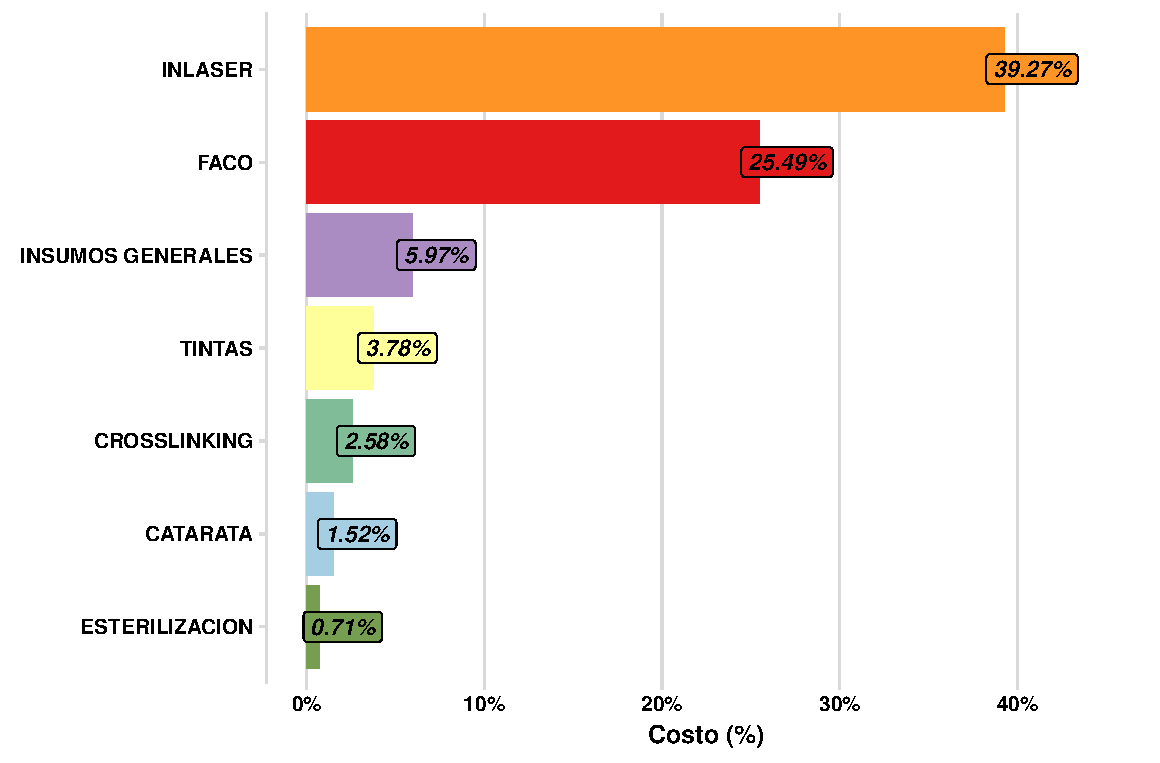
\includegraphics[width=15cm, height=10cm]{images/Especialidad.pdf}}
  \label{fig:EspecialidadGrupoA_almacen}
\end{figure}

La Figura \ref{fig:EspecialidadGrupoA_almacen} muestra un diagrama de barras de los productos seleccionados mediante el análisis ABC agrupados por especialidad y ordenados en base al porcentaje al costo, se observa que de los productos seleccionados para aplicar el modelo de inventarios lo que tienen la mayor parte de costos son de la especialidad de INLASER siendo el $39.27\%$ de los costos, seguido de FACO con el $25.49\%$ de costos, mientras que los productos con menor porcentaje son de la especialidad de CROSSLINKING, catarata y esterilización.

\newpage
\subsubsection{Descripción de los productos seleccionados}

\begin{longtable}{p{2cm} p{2cm} p{3.1cm} p{6.5cm}}
    \caption{Descripción de los productos seleccionados mediante la clasificacìón (ABC)}
    \label{table:ABC_productos_desc} \\
        \hline

        \hline
    \textbf{Código} & \textbf{Área} & \textbf{Subárea} & \textbf{Denominación} \\
        \hline
    \hline
    \endfirsthead

    \hline
    \textbf{Código} & \textbf{Área} & \textbf{Subárea} & \textbf{Denominación} \\
        \hline
    \hline
    %\multicolumn{5}{l}{\textbf{Independiente}} \\ % Se repite al inicio de cada nueva página
    \hline
    \endhead

    \hline
    \endfoot

    \hline
    \endlastfoot

        \hline
        \textbf{PROD001} & Oftalmología & INLASER & Paquete de tratamiento talla ``S'' \\
        \textbf{PROD002} & Oftalmología & FACO & KIT para procedimiento quirúrgico oftálmico (pack centurion ultra balance) \\
        \textbf{PROD003} & Oftalmología & FACO & Bolsa de solución BSS BAG 500 ml \\
        \textbf{PROD004} & Oftalmología & FACO & Cuchillo de hendidura CLEAR CUT HP2 2.4 mm bisel doble, intrepido sistema microcoaxial \\
        \textbf{PROD005} & Oftalmología & FACO & AJL VISC 1.4$\%$ - pack solución viscoelástica para uso intraocular hialuronato sódico 14 mg/ml canula 1x27g \\
        \textbf{PROD006} & Oftalmología & Insumos generales & Cuchillo lateral CLEAR CUT doble bisel 1.2 mm angulado \\
        \textbf{PROD007} & Oftalmología & CROSSLINKING & Solución de riboflavina VIBEX RAPID 0.1$\%$ isotonico jeringa de 1.5 ml \\
        \textbf{PROD008} & Oftalmología & INLASER & Anterior chamber cannula 27 g x 9 mm BEND \\
        \textbf{PROD009} & Oftalmología & FACO & Canula para cistotoma formada 27 g \\
        \textbf{PROD010} & Oftalmología & Tintas & Toner TNP80Y yellow para Konica Minolta BIZHUB C-3320i \\
        \textbf{PROD011} & Oftalmología & Insumos generales & Campo quirúrgico para ojos desechable 100 cm x 70 cm \\
        \textbf{PROD012} & Oftalmología & Tintas & Toner TNP80C cyan para Konica Minolta BIZHUB C-3320i \\
        \textbf{PROD013} & Oftalmología & Insumos generales & Lentes de contacto - AIR optix dia y noche \\
        \textbf{PROD014} & Oftalmología & Tintas & Toner Konica Minolta BIZHUB C-3320i Magenta \\
        \textbf{PROD015} & Oftalmología & Catarata & Solución salina equilibrada (BSS) en botella de vidrio 500 ml \\
        \textbf{PROD016} & Oftalmología & Insumos generales & Campo quirúrgico 100 x 120 cm \\
        \textbf{PROD017} & Oftalmología & Catarata & Azul de tripan 0.06$\%$ - 0.6 mg VIAL x 1 ml / OCUBLU - TRY \\
        \textbf{PROD018} & Oftalmología & Esterilización & Agua destilada y/o desionizada \\
        \hline
\end{longtable}

La Tabla \ref{table:ABC_productos_desc} muestra la descripción de los productos seleccionados mediante la clasificación (ABC), así como del área y subárea correspondiente. La mayor parte de las denominaciones vienen a ser instrumentos utilizados en las cirugías realizadas por el centro de salud integral ``La Fuente'' en el área de oftalmología; asimismo también se tienen productos utilizados por impresoras ya sea en la impresión de exámenes y evaluaciones realizadas.  

\section{Análisis de la demanda y selección del modelo}

Evaluando el KARDEX se tiene que los productos evaluados son mayormente derivados al área de sala de cirugías de oftalmología (a excepción de TINTAS), en el cual el área indica que el uso de los productos es según a las cirugías realizadas (cada producto utilizado para diferentes tipos de cirugías) no contando por el momento un registro de utilización de los productos, por el cual la estimación de la demanda de los productos se realizará en base a las cirugías realizadas del centro de salud en el año 2024.

Estableciendo un periodo de tiempo de 1 año tomando en cuenta las demandas mensuales en el año 2024 de los 18 productos seleccionados, se presenta la siguiente Tabla.

\newpage
\begin{landscape}

\begin{table}[H]
    \caption{Demanda mensual del año 2024 de los productos seleccionados}
    \footnotesize
    \begin{tabular}{p{1cm} >{\centering\arraybackslash}p{1.2cm} >{\centering\arraybackslash}p{1.2cm} >{\centering\arraybackslash}p{1.2cm} >{\centering\arraybackslash}p{1.2cm} >{\centering\arraybackslash}p{1.2cm} >{\centering\arraybackslash}p{1.2cm} >{\centering\arraybackslash}p{1.2cm} >{\centering\arraybackslash}p{1.2cm} >{\centering\arraybackslash}p{1.2cm} >{\centering\arraybackslash}p{1.2cm} >{\centering\arraybackslash}p{1.2cm} >{\centering\arraybackslash}p{1.2cm} } % Define anchos personalizados para cada columna
        \hline
        \textbf{Código} & \textbf{Enero} & \textbf{Febrero} & \textbf{Marzo} & \textbf{Abril} & \textbf{Mayo} & \textbf{Junio} & \textbf{Julio} & \textbf{Agosto} & \textbf{Setiembre} & \textbf{Octubre} & \textbf{Noviembre} & \textbf{Diciembre} \\
        \hline
        \textbf{PROD001} & 53 & 44 & 8 & 31 & 16 & 35 & 21 & 58 & 34 & 39 & 50 & 20 \\
        \textbf{PROD002} & 7 & 8 & 7 & 11 & 4 & 7 & 8 & 8 & 9 & 8 & 8 & 7 \\
        \textbf{PROD003} & 20 & 25 & 26 & 34 & 19 & 28 & 33 & 30 & 30 & 30 & 28 & 18 \\
        \textbf{PROD004} & 36 & 50 & 53 & 62 & 32 & 55 & 64 & 55 & 58 & 59 & 52 & 36 \\
        \textbf{PROD005} & 37 & 50 & 53 & 62 & 32 & 55 & 64 & 56 & 59 & 59 & 53 & 36 \\
        \textbf{PROD006} & 36 & 50 & 53 & 62 & 32 & 55 & 64 & 55 & 58 & 59 & 52 & 36 \\
        \textbf{PROD007} & 2 & 7 & 4 & 4 & 2 & 3 & 8 & 7 & 7 & 5 & 4 & 4 \\
        \textbf{PROD008} & 20 & 24 & 4 & 16 & 6 & 14 & 12 & 17 & 12 & 17 & 20 & 7 \\
        \textbf{PROD009} & 36 & 50 & 53 & 62 & 32 & 55 & 64 & 55 & 58 & 59 & 52 & 36 \\
        \textbf{PROD010} & 1 & 1 & 1 & 1 & 1 & 1 & 2 & 1 & 1 & 1 & 1 & 1 \\
        \textbf{PROD011} & 54 & 69 & 66 & 72 & 43 & 73 & 78 & 76 & 71 & 77 & 69 & 50 \\
        \textbf{PROD012} & 1 & 1 & 1 & 1 & 1 & 1 & 1 & 1 & 2 & 1 & 1 & 1 \\
        \textbf{PROD013} & 17 & 17 & 11 & 12 & 9 & 16 & 11 & 19 & 13 & 13 & 14 & 7 \\
        \textbf{PROD014} & 1 & 1 & 1 & 2 & 1 & 1 & 1 & 1 & 2 & 1 & 1 & 1 \\
        \textbf{PROD015} & 11 & 14 & 11 & 16 & 8 & 12 & 14 & 14 & 16 & 15 & 16 & 12 \\
        \textbf{PROD016} & 41 & 63 & 60 & 65 & 39 & 64 & 78 & 65 & 69 & 68 & 70 & 47 \\
        \textbf{PROD017} & 30 & 29 & 40 & 55 & 24 & 47 & 53 & 46 & 51 & 45 & 47 & 27 \\
        \textbf{PROD018} & 6 & 8 & 7 & 6 & 3 & 4 & 8 & 5 & 9 & 5 & 9 & 6 \\
        \hline
    \end{tabular}
    \label{table:Demanda_ABC_productos}
\end{table}

\end{landscape}

La Tabla \ref{table:Demanda_ABC_productos} muestra la demanda por los 12 meses de los productos seleccionados en el año 2024. 

Posteriormente se hallará el coeficiente de variabilidad ($CV$) mediante la ecuación (\ref{CVar}), como asi mismo se determinará el modelo de inventarios adecuado.

\begin{table}[H]
    \caption{Coeficiente de variabilidad y modelo de inventarios de los productos seleccionados}
    \begin{tabular}{p{2cm} p{2cm} p{2cm} p{2cm} p{2cm} p{2.5cm}} % Define anchos personalizados para cada columna
        \hline
        \textbf{Código} & \textbf{Total} & \textbf{$Media$} & \textbf{$Varianza$} & \textbf{$CV$} & \textbf{Modelo} \\
        \hline
        \textbf{PROD001} & 409 & $34.08$ & $224.41$ & $0.19$ & \textbf{Determinístico} \\
        \textbf{PROD002} & 92 & $7.67$ & $2.39$ & $0.04$ & \textbf{Determinístico} \\
        \textbf{PROD003} & 321 & $26.75$ & $26.02$ & $0.04$ & \textbf{Determinístico} \\
        \textbf{PROD004} & 612 & $51.00$ & $104.33$ & $0.04$ & \textbf{Determinístico} \\
        \textbf{PROD005} & 616 & $51.33$ & $104.06$ & $0.04$ & \textbf{Determinístico} \\
        \textbf{PROD006} & 612 & $51.00$ & $104.33$ & $0.04$ & \textbf{Determinístico} \\
        \textbf{PROD007} & 57 & $4.75$ & $3.85$ & $0.17$ & \textbf{Determinístico} \\
        \textbf{PROD008} & 169 & $14.08$ & $34.58$ & $0.17$ & \textbf{Determinístico} \\
        \textbf{PROD009} & 612 & $51.00$ & $104.33$ & $0.04$ & \textbf{Determinístico} \\
        \textbf{PROD010} & 13 & $1.08$ & $0.08$ & $0.07$ & \textbf{Determinístico} \\
        \textbf{PROD011} & 798 & $66.50$ & $118.25$ & $0.03$ & \textbf{Determinístico} \\
        \textbf{PROD012} & 13 & $1.08$ & $0.08$ & $0.07$ & \textbf{Determinístico} \\
        \textbf{PROD013} & 159 & $13.25$ & $11.52$ & $0.07$ & \textbf{Determinístico} \\
        \textbf{PROD014} & 14 & $1.17$ & $0.14$ & $0.10$ & \textbf{Determinístico} \\
        \textbf{PROD015} & 159 & $13.25$ & $5.69$ & $0.03$ & \textbf{Determinístico} \\
        \textbf{PROD016} & 729 & $60.75$ & $134.02$ & $0.04$ & \textbf{Determinístico} \\
        \textbf{PROD017} & 494 & $41.17$ & $108.64$ & $0.06$ & \textbf{Determinístico} \\
        \textbf{PROD018} & 76 & $6.33$ & $3.39$ & $0.08$ & \textbf{Determinístico} \\
        \hline
    \end{tabular}
    \label{table:GrupoA_Area}
\end{table}

La Tabla \ref{table:GrupoA_Area} muestra el coeficiente de variabilidad calculado para los productos seleccionados. Donde se muestra que todos los productos tienen una demanda determinística ya que su coeficiente de variabilidad es menor a 0.20 en lo que se usará un modelo determinístico de inventarios.

\section{Determinación de costos}

Procedamos a recopilar la información de los costos. El área de administración y logística proporcionó la información de compras y factores asociados al almacén del centro de salud. Para esta parte tomemos los productos seleccionados mediante el análisis ABC presentado en la sección anterior, seguidamente hallemos los costos específicos de cada producto, que se presentará en cada subsección a continuación, de la misma forma será en tamaño de su ocupación en el área de almacén, que se presenta en la siguiente Tabla.

\begin{table}[H]
    \caption{Ocupación de los productos seleccionados mediante el análisis ABC}
    \begin{tabular}{p{2cm} p{3cm} p{5cm}} % Define anchos personalizados para cada columna
        \hline
        \textbf{Código} & \textbf{Volumen ($cm^3$)} & \textbf{Proporción en almacén} \\
        \hline
        \textbf{PROD001} & 42400 & $0.3367\%$ \\
        \textbf{PROD002} & 63920 & $0.5077\%$ \\
        \textbf{PROD003} & 140296 & $1.1142\%$ \\
        \textbf{PROD004} & 28800 & $0.2287\%$ \\
        \textbf{PROD005} & 52800 & $0.4193\%$ \\
        \textbf{PROD006} & 54720 & $0.4346\%$ \\
        \textbf{PROD007} & 30720 & $0.2440\%$ \\
        \textbf{PROD008} & 57600 & $0.4575\%$ \\
        \textbf{PROD009} & 40700 & $0.3232\%$ \\
        \textbf{PROD010} & 36000 & $0.2859\%$ \\
        \textbf{PROD011} & 92800 & $0.7370\%$ \\
        \textbf{PROD012} & 36000 & $0.2859\%$ \\
        \textbf{PROD013} & 29700 & $0.2359\%$ \\
        \textbf{PROD014} & 36000 & $0.2859\%$ \\
        \textbf{PROD015} & 85280 & $0.6773\%$ \\
        \textbf{PROD016} & 10640 & $0.0845\%$ \\
        \textbf{PROD017} & 10800 & $0.0858\%$ \\
        \textbf{PROD018} & 2228696 & $17.70\%$ \\
        \hline
    \end{tabular}
    \label{table:GrupoA_Ocupacion}
\end{table}

La Tabla \ref{table:GrupoA_Ocupacion} muestra los productos seleccionados con respecto a la dimensión que ocupa en el área de almacén. El volumen considera el espacio que se esta asignando para cada producto de almacén independientemente si los productos ocupan todo o parte del espacio asignado. No se mostraron costos de escasez ya que se tuvieron todos los productos para satisfacer la demanda en el año 2024, por lo que se tomarán los costos de compra, costo de preparación y costo de almacenamiento.

\subsection{Costo de compra}
Como se definió en la ecuación (\ref{2.1}) este viene a ser los costos por unidad de cada artículo del inventario, en el cual se debe incluir costos de descuento. En la política de inventario el costo de compra no influye, pero si influye en el costo total de cada producto.

Para determinar este costo, se tomó en cuenta el KARDEX de logística en el cual se precisa el precio unitario de cada producto. Mediante la consulta al área de logística se indicó que los precios de cada producto ya son determinados de manera fija por previo acuerdo con el proveedor independiente de un descuento por cantidad, asimismo este precio de pedido también incluye el precio de transporte. Lo que indica que los precios de compra son únicamente los precios unitarios de cada producto registrado en el KARDEX resumido de la siguiente forma:
\begin{itemize}
\item \textbf{Costo de compra:} Costo de adquirir el producto, de manera fija con previo acuerdo del proveedor por lo que no tiene descuento.
\item \textbf{Costo de transporte:} No esta incluido ya que el acuerdo de pedido es independiente a los costos de transporte, es decir se puede realizar el pedido de $n$ productos sin necesidad de que haya un costo adicional de transporte.
\end{itemize}

La información de los productos seleccionados mediante el análisis ABC se muestra en la siguiente Tabla.

\newpage
\begin{table}[H]
    \caption{Costos de compra de los productos seleccionados mediante el análisis ABC}
    \begin{tabular}{p{2cm} p{5cm} p{6.5cm}} % Define anchos personalizados para cada columna
        \hline
        \textbf{Código} & \textbf{Costo Unitario (S/)} & \textbf{Costo total del año 2024 (S/)} \\
        \hline
        \textbf{PROD001} & S/ 4,282.68 & S/ 165,471.40 \\
        \textbf{PROD002} & S/ 542.60 & S/ 49,666.90 \\
        \textbf{PROD003} & S/ 345.15 & S/ 21,532.12 \\
        \textbf{PROD004} & S/ 69.80 & S/ 17,572.86 \\
        \textbf{PROD005} & S/ 90.00 & S/ 17,100.00 \\
        \textbf{PROD006} & S/ 72.81 & S/ 11,828.01 \\
        \textbf{PROD007} & S/ 362.94 & S/ 11,370.00 \\
        \textbf{PROD008} & S/ 16.00 & S/ 7,680.00 \\
        \textbf{PROD009} & S/ 143.00 & S/ 6,507.00 \\
        \textbf{PROD010} & S/ 720.00 & S/ 6,498.00 \\
        \textbf{PROD011} & S/ 15.59 & S/ 6,259.82 \\
        \textbf{PROD012} & S/ 715.00 & S/ 5,839.00 \\
        \textbf{PROD013} & S/ 143.37 & S/ 4,874.58 \\
        \textbf{PROD014} & S/ 715.00 & S/ 4,337.00 \\
        \textbf{PROD015} & S/ 290.00 & S/ 3,480.00 \\
        \textbf{PROD016} & S/ 14.00 & S/ 3,346.00 \\
        \textbf{PROD017} & S/ 400.00 & S/ 3,200.00 \\
        \textbf{PROD018} & S/ 39.84 & S/ 3,132.82 \\
        \hline
    \end{tabular}
    \label{table:GrupoA_Costo_Compra}
\end{table}

La Tabla \ref{table:GrupoA_Costo_Compra} muestra los costos de compra que debe tener cada producto según el KARDEX, asimismo también se muestra el costo de compra total que se realizó en el año 2024.

\subsection{Costo de preparación}

Como se definió en la ecuación (\ref{2.1}) este viene a ser los costos que incurren cuando se coloca un pedido, es decir los costos de las operaciones realizadas al momento de realizar el pedido del producto independiente de su tamaño o cantidad solicitada. Según la información brindada por el área de administración y logística estos costos estaría en base a los siguientes conceptos:

\begin{itemize}
\item \textbf{Sueldo:} En el cual el centro de salud asumen un costo mensual por el tiempo que dedica el trabajador a las funciones involucradas al pedido de productos. Este costo es determinada por el área de administración en base al porcentaje de la función y su sueldo mensual, en la cual están involucrados 4 personales de logística directamente, el resultado se muestra en la siguiente Tabla.

\begin{table}[H]
    \caption{Costo de sueldos en base a costos de preparación}
    \begin{tabular}{p{5cm} p{8cm}} % Define anchos personalizados para cada columna
        \hline
        \textbf{Personal} & \textbf{Costo preparación personal (S/)} \\
        \hline
        \textbf{Logística (personal 1)} & S/ 18.00 \\
        \textbf{Logística (personal 2)} & S/ 25.00 \\
        \textbf{Logística (personal 3)} & S/ 23.00 \\
        \textbf{Logística (personal 4)} & S/ 5.65 \\
        \hline
        \textbf{Total} & S/ 71.65
    \end{tabular}
    \label{table:Personal_costo_preparacion}
\end{table}

La Tabla \ref{table:Personal_costo_preparacion} muestra los sueldos por mes del personal involucrado con respecto a las funciones por costo de preparación, en la que se tiene un total de S/ 71.65 por mes y en el año sería de S/ 859.80

\item \textbf{Servicio de telefonía móvil:} Para realizar los pedidos son necesarios el servicio de telefonía móvil e internet para realizar el pedido. Ya que el costo del servicio no es exclusivamente para los pedidos, en cambio viene a ser un costo general que recibe el centro de salud integral, es necesario estimarlo en base al área útil que ocupa el área de trabajo de almacén, en el cual se tiene una área útil total de 1260.38$m^2(100\%)$, en el cual el área útil de almacén es de 19.92$m^2(1.58\%)$. Entonces tomando en cuenta que el servicio de telefonía móvil anual es de S/ 5,772.16 con respecto al área útil de almacén $(1.58\%)$ se tiene un costo de servicio para preparación de S/ 91.20 anual.

\end{itemize}

Por lo que tomando estos dos costos, se tiene un costo de preparación por servicios de S/ 91.20 y un costo de preparación por personal de S/ 859.80, en el que sumando ambos costos se tiene un costo de preparación de S/ 951.00 que viene a ser de todo almacén. Si tomamos este precio en base a la proporción de pedidos realizados en el año 2024 se tendría el costo de preparación, la información de la cantidad de pedidos realizados se obtendrá mediante el KARDEX de logística y las órdenes realizadas. La siguiente Tabla resume estos valores para los productos seleccionados mediante el análisis ABC.

\begin{table}[H]
    \caption{Costos de preparación de los productos seleccionados mediante el análisis ABC}
    \begin{tabular}{p{2cm} p{1.5cm} p{5.5cm} p{5cm}} % Define anchos personalizados para cada columna
        \hline
        \textbf{Código} & \textbf{Pedidos} & \textbf{Proporción Pedidos ($\%$)} & \textbf{Costo de preparación (S/)} \\
        \hline
        \textbf{PROD001} & 2 & $0.40\%$ & S/ 3.80 \\
        \textbf{PROD002} & 9 & $1.82\%$ & S/ 17.31 \\
        \textbf{PROD003} & 10 & $2.02\%$ & S/ 19.21 \\
        \textbf{PROD004} & 5 & $1.01\%$ & S/ 9.61 \\
        \textbf{PROD005} & 4 & $0.81\%$ & S/ 7.70 \\
        \textbf{PROD006} & 2 & $0.40\%$ & S/ 3.80 \\
        \textbf{PROD007} & 1 & $0.20\%$ & S/ 1.90 \\
        \textbf{PROD008} & 4 & $0.81\%$ & S/ 7.70 \\
        \textbf{PROD009} & 5 & $1.01\%$ & S/ 9.61 \\
        \textbf{PROD010} & 6 & $1.21\%$ & S/ 11.51 \\
        \textbf{PROD011} & 7 & $1.42\%$ & S/ 13.50 \\
        \textbf{PROD012} & 8 & $1.62\%$ & S/ 15.41 \\
        \textbf{PROD013} & 1 & $0.20\%$ & S/ 1.90 \\
        \textbf{PROD014} & 5 & $1.01\%$ & S/ 9.61 \\
        \textbf{PROD015} & 3 & $0.61\%$ & S/ 5.80 \\
        \textbf{PROD016} & 2 & $0.40\%$ & S/ 3.80 \\
        \textbf{PROD017} & 5 & $1.01\%$ & S/ 9.61 \\
        \textbf{PROD018} & 6 & $1.21\%$ & S/ 11.51 \\
        \hline
    \end{tabular}
    \label{table:GrupoA_Costo_Preparacion}
\end{table}

La Tabla \ref{table:GrupoA_Costo_Preparacion} muestra los pedidos realizados, la proporción de los pedidos tomando en cuenta los pedidos de todos los productos de almacén y también se muestra el costo de preparación de cada producto.

\subsection{Costo de retención}
Como se definió en la ecuación (\ref{2.1}) este viene a ser los costos que se realizan al mantener la existencia de productos sobrantes, es decir los costos de almacenamiento, mantenimiento y manejo del producto. Según la información brindada por el área de administración y logística estos costos estaría en base a los siguientes conceptos:

\begin{itemize}
\item \textbf{Sueldo:} En el cual el centro de salud asume un costo mensual por el tiempo que dedica el trabajador a las funciones involucradas al mantenimiento de productos. Este costo es determinada por el área de administración en base al porcentaje de la función y su sueldo mensual, en la cual están involucrado 1 personal de limpieza y mantenimiento y 1 personal de seguridad directamente, el resultado se muestra en la siguiente Tabla.

\begin{table}[H]
    \caption{Costo de servicios en base a costos de retención}
    \begin{tabular}{p{5cm} p{8cm}} % Define anchos personalizados para cada columna
        \hline
        \textbf{Personal} & \textbf{Costo retención personal (S/)} \\
        \hline
        \textbf{Seguridad} & S/ 84.80 \\
        \textbf{Limpieza} & S/ 68.90 \\
        \hline
        \textbf{Total} & S/ 153.70
    \end{tabular}
    \label{table:Personal_costo_retencion}
\end{table}

La Tabla \ref{table:Personal_costo_retencion} muestra los sueldos del personal respecto a retención de S/ 153.70 por mes por lo que al año sería de S/ 1,844.40

\item \textbf{Servicios:} Para realizar el adecuado almacenamiento de los productos se necesitan de servicios de energía eléctrica y agua por lo que para los costos de retención se tomará en base al área útil que ocupa el área útil de almacén que es 19.92$m^2(1.58\%)$.

\begin{table}[H]
    \caption{Costo de sueldos en base a costos de retención}
    \begin{tabular}{p{4cm} p{4cm} p{4cm}}
        \hline
        \textbf{Servicio} & \textbf{Total ($100\%$)} & \textbf{Almacén ($1.58\%$)} \\
        \hline
        \textbf{Luz o energía eléctrica} & S/ 51,719.70 & S/ 817.70 \\
        \textbf{Agua} & S/ 789.31 & S/ 12.47 \\
        \hline
        \multicolumn{2}{c}{\textbf{Total}} & S/ 830.17
    \end{tabular}
    \label{table:Servicio_costo_retencion}
\end{table}

\end{itemize}

Por lo que tomando estos dos costos, se tiene un costo de retención por servicios de S/ 830.17 y un costo de retención por personal de S/ 1,844.40, en el que sumando ambos costos se tiene un costo de retención de S/ 2,674.57 que viene a ser de todo almacén. Si tomamos este precio en base a la proporción del espacio que ocupa cada producto se tendría el costo de retención, la información del volumen que ocupa cada producto sera medido del área de almacén. La siguiente Tabla resume estos valores para los productos seleccionados mediante el análisis ABC.

\begin{table}[H]
    \caption{Costos de retención de los productos seleccionados mediante el análisis ABC}
    \begin{tabular}{p{2cm} p{2.7cm} p{4.5cm} p{4.3cm}} % Define anchos personalizados para cada columna
        \hline
        \textbf{Código} & \textbf{Volumen ($cm^3$)} & \textbf{Proporción Volumen ($\%$)} & \textbf{Costo de retención (S/)} \\
        \hline
        \textbf{PROD001} & 42400 & $0.34\%$ & S/ 9.90 \\
        \textbf{PROD002} & 63920 & $0.51\%$ & S/ 13.64 \\
        \textbf{PROD003} & 140296 & $1.11\%$ & S/ 29.42 \\
        \textbf{PROD004} & 28800 & $0.23\%$ & S/ 6.15 \\
        \textbf{PROD005} & 52800 & $0.42\%$ & S/ 11.23 \\
        \textbf{PROD006} & 54720 & $0.43\%$ & S/ 11.50 \\
        \textbf{PROD007} & 30720 & $0.24\%$ & S/ 6.42 \\
        \textbf{PROD008} & 57600 & $0.46\%$ & S/ 12.30 \\
        \textbf{PROD009} & 40700 & $0.32\%$ & S/ 8.56 \\
        \textbf{PROD010} & 36000 & $0.29\%$ & S/ 7.76 \\
        \textbf{PROD011} & 92800 & $0.74\%$ & S/ 19.79 \\
        \textbf{PROD012} & 36000 & $0.29\%$ & S/ 7.76 \\
        \textbf{PROD013} & 29700 & $0.24\%$ & S/ 6.42 \\
        \textbf{PROD014} & 36000 & $0.29\%$ & S/ 7.76 \\
        \textbf{PROD015} & 85280 & $0.68\%$ & S/ 18.19 \\
        \textbf{PROD016} & 10640 & $0.08\%$ & S/ 2.14 \\
        \textbf{PROD017} & 10800 & $0.09\%$ & S/ 2.41 \\
        \textbf{PROD018} & 2228696 & $17.70\%$ & S/ 473.40 \\
        \hline
    \end{tabular}
    \label{table:GrupoA_Costo_Retencion}
\end{table}

La Tabla \ref{table:GrupoA_Costo_Retencion} muestra el volumen que ocupa cada producto, la proporción del volumen tomando en cuenta todos los productos de almacén, y también se muestra el costo de retención de cada producto.
\section{Políticas de inventario}

Tomando en cuenta el modelo seleccionado a través de la demanda, los costos de compra, preparación y retención mostrada en el capitulo anterior. Se procederá con la descripción de los productos seleccionados en base a la tendencia y la aplicación del modelo de inventarios seleccionado para generar una política de inventarios óptima.

\subsection{Política de inventarios para los productos seleccionados mediante el análisis ABC}

En este apartado se realizará el modelo de inventarios de los productos seleccionados, empezando realizando un análisis de su demanda, aplicación del modelo de inventarios y finalmente hallando la política de inventarios óptima.
\subsubsection{Paquete de tratamiento talla ``S''}
El primer producto a evaluar es el Paquete de tratamiento talla ``S'' de INLASER del área de oftalmología. Este insumo es utilizado para las cirugías refractivas, primeramente observemos la tendencia de la demanda a lo largo del año 2024 en el siguiente gráfico.
\begin{figure}[H]
  \caption{Evolución demanda: Paquete de tratamiento talla ``S'' de INLASER - Oftalmología en el año 2024}
  {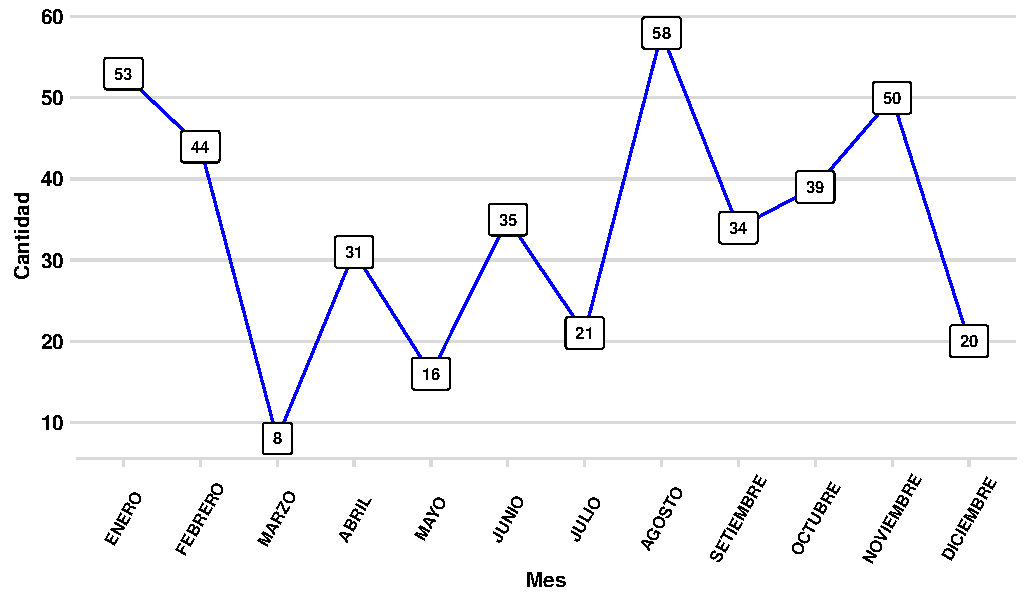
\includegraphics[width=15cm, height=5.95cm]{images/PROD001_demanda.pdf}}
  \label{fig:PROD001_demanda}
\end{figure}
La Figura \ref{fig:PROD001_demanda} muestra el diagrama de lineas que representa la evolución de la demanda del paquete de tratamiento talla ``S'' por mes en el año 2024, se observa que la demanda tiene un comportamiento determinístico a través de los meses del año, a excepción del mes de marzo y agosto donde hubo puntos extremos, asimismo no se observa una tendencia y solo estacionariedad en el tiempo, por lo que tomando estos casos y el comportamiento de la demanda es necesario utilizar un \textsl{modelo determinístico EOQ}.

Tomando en cuenta la demanda total anual de la Tabla \ref{table:GrupoA_Area}, el costo de compra de la Tabla \ref{table:GrupoA_Costo_Compra}, el costo de preparación estimado de la Tabla \ref{table:GrupoA_Costo_Preparacion}, el costo de retención estimado de la Tabla \ref{table:GrupoA_Costo_Retencion} y tiempo de reabastecimiento del pedido brindado por el área de logística se tienen los siguientes valores:
\begin{itemize}
    \item \textbf{Demanda ($D$):} 409 unidades
    \item \textbf{Costo de compra ($C$):} S/ 4,282.68 por unidad
    \item \textbf{Costo de preparación ($K$):} S/ 3.80
    \item \textbf{Costo de retención ($h$):} S/ 9.90
    \item \textbf{Tiempo de entrega ($L$):} 7 días
\end{itemize}
Hallamos la cantidad de pedido óptima $y^*$ mediante la expresión (\ref{yopt}) de la siguiente manera
\begin{eqnarray}
    y^* &=& \sqrt{\frac{2KD}{h}} \nonumber \\
    y^* &=& \sqrt{\frac{2(3.8)(409)}{9.90}} \nonumber \\
    y^* &=& 17.72 \nonumber \\
    y^* &\thickapprox& 18 \text{ unidades} \nonumber
\end{eqnarray}
De la misma forma hallemos el intervalo de pedido óptimo $T^*$ utilizando la expresión (\ref{Topt}) 
\begin{eqnarray}
    T^* &=& \sqrt{\frac{2K}{Dh}} \nonumber \\
    T^* &=& \sqrt{\frac{2(3.8)}{(409)(9.9)}} \nonumber \\
    T^* &=& 0.0433 \nonumber
\end{eqnarray}
Asimismo tomemos la demanda por día laborable (52 semanas * 5 días/semana = 260 días laborables) de tal forma que vemos el momento de cuando pedir
\begin{eqnarray}
    T^* &=& 0.0433 (260 \text{ días laborables}) \nonumber \\   
    T^* &=& 11.26 \nonumber \\
    T^* &\thickapprox& 11 \text{ días laborables} \nonumber
\end{eqnarray}
Ahora hallemos el costo mínimo total de inventario óptimo $CTI(y^*)$ usando la expresión (\ref{CTIopt}).
\begin{eqnarray}
    CTI(y^*) &=& \sqrt{2hKD} + DC \nonumber \\
    CTI(y^*) &=& \sqrt{2(9.9)(3.8)(409)} + (409)(4282.68) \nonumber \\
    CTI(y^*) &=& \text{S/ 1,751,791.54} \nonumber
\end{eqnarray}
Por último hallemos el punto de reorden en base a la cantidad de pedido óptima y el tiempo de reabastecimiento de 7 días.
\begin{eqnarray}
    R &=& L_e D \nonumber \\
    R &=& (7) \left(\frac{409}{260 \text{ días laborables}} \right) \nonumber \\
    R &=& 11.01 \nonumber \\
    R &\thickapprox& 11 \text{ unidades} \nonumber
\end{eqnarray}
Esto quiere decir que cuando el inventario del producto llegue a 11 unidades se deben de realizar el pedido de 18 unidades, del cual el tiempo de pedido debería ser cada 11 días laborables teniendo un costo total de S/ 1,751,791.54
\subsubsection{KIT para procedimiento quirúrgico oftálmico (pack centurion ultra balance)}
El producto KIT para procedimiento quirúrgico oftálmico (pack centurion ultra balance) de FACO del área de oftalmología es utilizado para las cirugía de facoemulsificación para la extracción de la catarata, observemos la tendencia de la demanda a lo largo del año 2024.
\clearpage
\begin{figure}[H]
  \caption{Evolución demanda: KIT para procedimiento quirúrgico oftálmico (pack centurion ultra balance) de FACO - oftalmología}
  {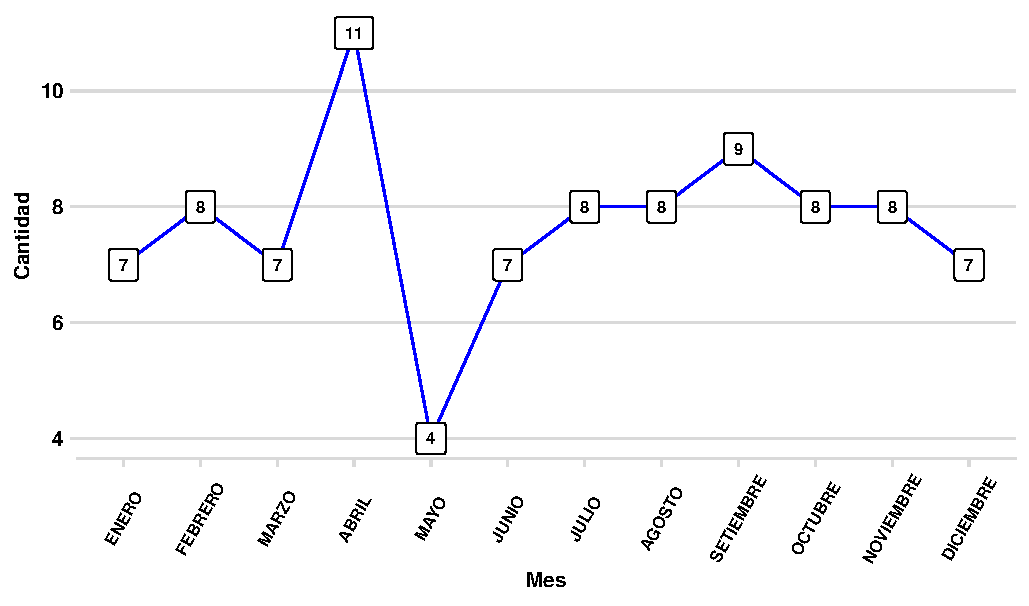
\includegraphics[width=15cm, height=5.95cm]{images/PROD002_demanda.pdf}}
  \label{fig:PROD002_demanda}
\end{figure}
La Figura \ref{fig:PROD002_demanda} muestra el diagrama de lineas que representa la evolución de la demanda del KIT para procedimiento quirúrgico oftálmico por mes en el año 2024, se observa que la demanda tiene un comportamiento determinístico a través de los meses del año, a excepción del mes de abril y mayo donde hubo puntos extremos, asimismo no se observa una tendencia y solo estacionariedad en el tiempo, por lo que tomando estos casos y el comportamiento de la demanda es necesario utilizar un \textsl{modelo determinístico EOQ}.

Tomando en cuenta la demanda total anual de la Tabla \ref{table:GrupoA_Area}, el costo de compra de la Tabla \ref{table:GrupoA_Costo_Compra}, el costo de preparación estimado de la Tabla \ref{table:GrupoA_Costo_Preparacion}, el costo de retención estimado de la Tabla \ref{table:GrupoA_Costo_Retencion} y tiempo de reabastecimiento del pedido brindado por el área de logística se tienen los siguientes valores:

\begin{itemize}
    \item \textbf{Demanda ($D$):} 92 unidades
    \item \textbf{Costo de compra ($C$):} S/ 542.60 por unidad
    \item \textbf{Costo de preparación ($K$):} S/ 17.31
    \item \textbf{Costo de retención ($h$):} S/ 13.64
    \item \textbf{Tiempo de entrega ($L$):} 3 días
\end{itemize}

Hallamos la cantidad de pedido óptima $y^*$ mediante la expresión (\ref{yopt}) de la siguiente manera
\begin{eqnarray}
    y^* &=& \sqrt{\frac{2KD}{h}} \nonumber \\
    y^* &=& \sqrt{\frac{2(17.31)(92)}{13.64}} \nonumber \\
    y^* &=& 15.28 \nonumber \\
    y^* &\thickapprox& 15 \text{ unidades} \nonumber
\end{eqnarray}
De la misma forma hallemos el intervalo de pedido óptimo $T^*$ utilizando la expresión (\ref{Topt}) 
\begin{eqnarray}
    T^* &=& \sqrt{\frac{2K}{Dh}} \nonumber \\
    T^* &=& \sqrt{\frac{2(17.31)}{(92)(13.64)}} \nonumber \\
    T^* &=& 0.1661 \nonumber
\end{eqnarray}
Asimismo tomemos la demanda por día laborable (52 semanas * 5 días/semana = 260 días laborables) de tal forma que vemos el momento de cuando pedir
\begin{eqnarray}
    T^* &=& 0.1661 (260 \text{ días laborables}) \nonumber \\   
    T^* &=& 43.19 \nonumber \\
    T^* &\thickapprox& 43 \text{ días laborables} \nonumber
\end{eqnarray}
Ahora hallemos el costo mínimo total de inventario óptimo $CTI(y^*)$ usando la expresión (\ref{CTIopt}).
\begin{eqnarray}
    CTI(y^*) &=& \sqrt{2hKD} + DC \nonumber \\
    CTI(y^*) &=& \sqrt{2(13.64)(17.31)(92)} + (92)(542.60) \nonumber \\
    CTI(y^*) &=& \text{S/ 50,127.63} \nonumber
\end{eqnarray}
Por último hallemos el punto de reorden en base a la cantidad de pedido óptima y el tiempo de reabastecimiento de 3 días.

\begin{eqnarray}
    R &=& L_e D \nonumber \\
  R &=& (3) \left(\frac{92}{260\text{ días laborables }} \right) \nonumber \\
  R &=& 1.06 \nonumber \\
  R &\thickapprox& 1\text{ unidad}
\end{eqnarray}

Esto quiere decir que cuando el inventario del producto llegue a 1 unidad se deben de realizar el pedido de 15 unidades, del cual el tiempo de pedido debería ser cada 43 días laborables teniendo un costo total de S/ 50,127.63
\subsubsection{Bolsa de solución BSS BAG 500 ml}

El producto bolsa de solución BSS BAG 500 ml de FACO del área de oftalmología es utilizado para las cirugía de facoemulsificación para la extracción de la catarata, primeramente observemos la tendencia de la demanda a lo largo del año 2024 en el siguiente gráfico.

\begin{figure}[H]
  \caption{Evolución demanda: Bolsa de solución BSS BAG 500 ml de FACO - oftalmología}
  {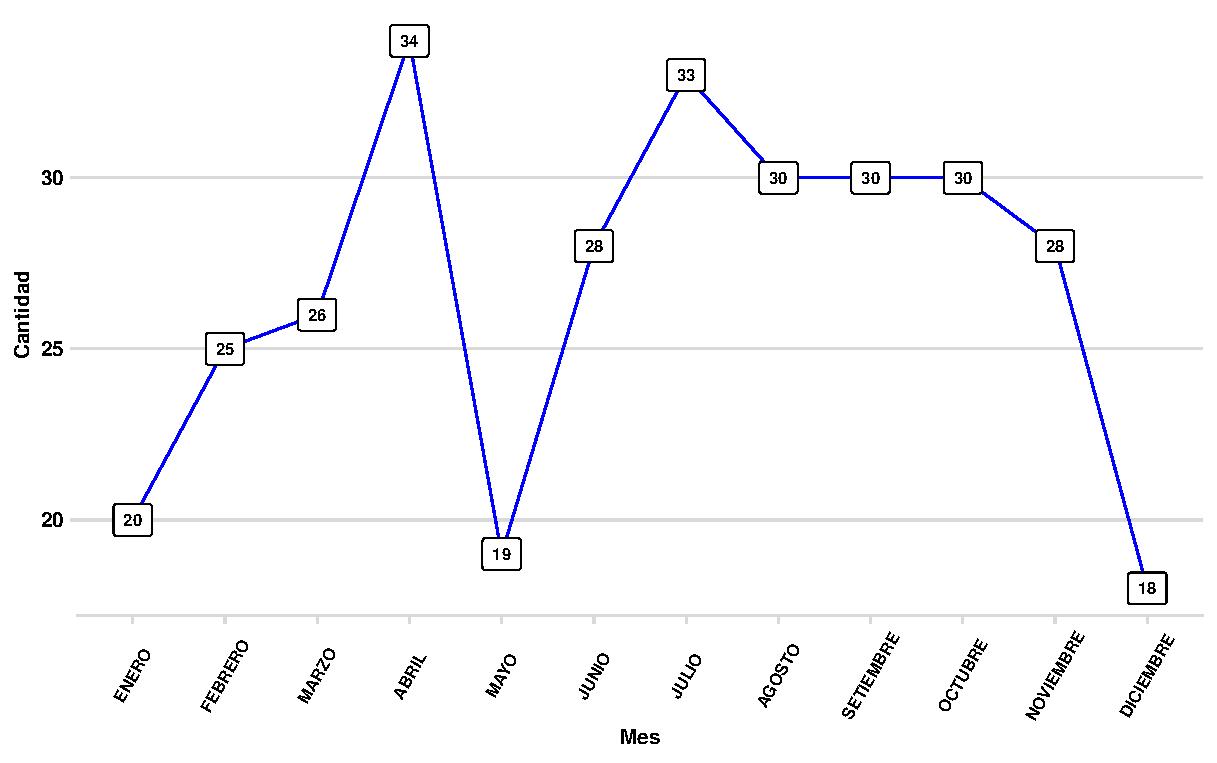
\includegraphics[width=15cm, height=5.95cm]{images/PROD003_demanda.pdf}}
  \label{fig:PROD003_demanda}
\end{figure}

La Figura \ref{fig:PROD003_demanda} muestra el diagrama de lineas que representa la evolución de la demanda de la bolsa de solución BSS BAG 500 ml por mes en el año 2024, se observa que la demanda tiene un comportamiento determinístico a través de los meses del año, a excepción del mes de enero, mayo y diciembre en donde hubo puntos extremos, asimismo no se observa una tendencia y solo estacionariedad en el tiempo, por lo que tomando estos casos y el comportamiento de la demanda es necesario utilizar un \textsl{modelo determinístico EOQ}.

Tomando en cuenta la demanda total anual de la Tabla \ref{table:GrupoA_Area}, el costo de compra de la Tabla \ref{table:GrupoA_Costo_Compra}, el costo de preparación estimado de la Tabla \ref{table:GrupoA_Costo_Preparacion}, el costo de retención estimado de la Tabla \ref{table:GrupoA_Costo_Retencion} y tiempo de reabastecimiento del pedido brindado por el área de logística se tienen los siguientes valores:

\begin{itemize}
    \item \textbf{Demanda ($D$):} 321 unidades
    \item \textbf{Costo de compra ($C$):} S/ 345.15 por unidad
    \item \textbf{Costo de preparación ($K$):} S/ 19.21
    \item \textbf{Costo de retención ($h$):} S/ 29.42
    \item \textbf{Tiempo de entrega ($L$):} 3 días
\end{itemize}

Hallamos la cantidad de pedido óptima $y^*$ mediante la expresión (\ref{yopt}) de la siguiente manera
\begin{eqnarray}
    y^* &=& \sqrt{\frac{2KD}{h}} \nonumber \\
    y^* &=& \sqrt{\frac{2(19.21)(321)}{29.42}} \nonumber \\
    y^* &=& 20.47 \nonumber \\
    y^* &\thickapprox& 20 \text{ unidades} \nonumber
\end{eqnarray}
De la misma forma hallemos el intervalo de pedido óptimo $T^*$ utilizando la expresión (\ref{Topt}) 
\begin{eqnarray}
    T^* &=& \sqrt{\frac{2K}{Dh}} \nonumber \\
    T^* &=& \sqrt{\frac{2(19.21)}{(321)(29.42)}} \nonumber \\
    T^* &=& 0.0638 \nonumber
\end{eqnarray}
Asimismo tomemos la demanda por día laborable (52 semanas * 5 días/semana = 260 días laborables) de tal forma que vemos el momento de cuando pedir

\begin{eqnarray}
    T^* &=& 0.0638 (260 \text{ días laborables}) \nonumber \\   
    T^* &=& 16.58 \nonumber \\
    T^* &\thickapprox& 17 \text{ días laborables} \nonumber
\end{eqnarray}
Ahora hallemos el costo mínimo total de inventario óptimo $CTI(y^*)$ usando la expresión (\ref{CTIopt}).
\begin{eqnarray}
    CTI(y^*) &=& \sqrt{2hKD} + DC \nonumber \\
    CTI(y^*) &=& \sqrt{2(29.42)(19.21)(321)} + (321)(345.15) \nonumber \\
    CTI(y^*) &=& \text{S/ 111,395.51} \nonumber
\end{eqnarray}
Por último hallemos el punto de reorden en base a la cantidad de pedido óptima y el tiempo de reabastecimiento de 3 días.
\begin{eqnarray}
    R &=& L_e D \nonumber \\
    R &=& (3) \left(\frac{321}{260 \text{ días laborables}} \right) \nonumber \\
    R &=& 3.70 \nonumber \\
    R &\thickapprox& 4 \text{ unidades} \nonumber
\end{eqnarray}

Esto quiere decir que cuando el inventario del producto llegue a 4 unidades se deben de realizar el pedido de 20 unidades, del cual el tiempo de pedido debería ser cada 17 días laborables teniendo un costo total de S/ 111,395.51
\subsubsection{Cuchillo de hendidura CLEAR CUT HP2 2.4 mm bisel doble, intrepido sistema microcoaxial}

El producto cuchillo de hendidura CLEAR CUT HP2 2.4 mm bisel doble, intrepido sistema microcoaxial de FACO del área de oftalmología es utilizado para las cirugía de facoemulsificación y extracción manual de catarata con incisión pequeña que son las cirugías para la extracción de la catarata, primeramente observemos la tendencia de la demanda a lo largo del año 2024 en el siguiente gráfico.

\begin{figure}[H]
  \caption{Evolución demanda: Cuchillo de hendidura CLEAR CUT HP2 2.4 mm bisel doble, intrepido sistema microcoaxial de FACO - oftalmología}
  {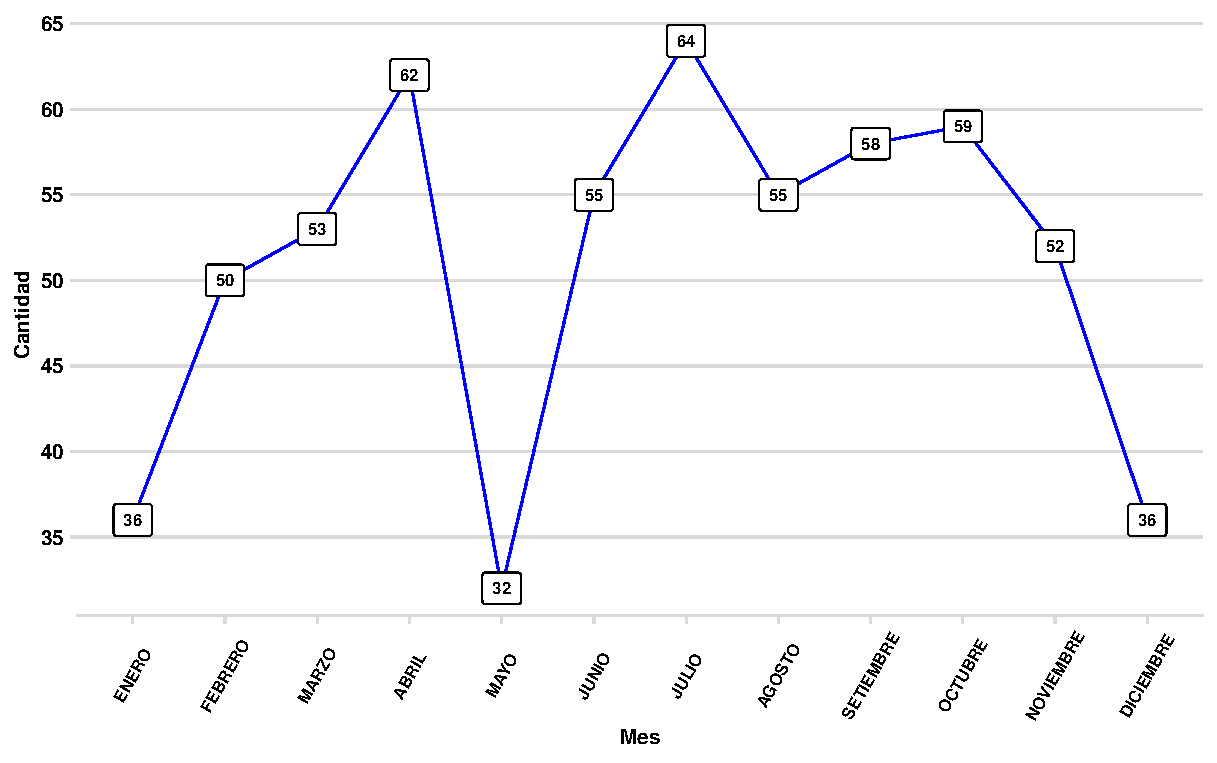
\includegraphics[width=15cm, height=5.95cm]{images/PROD004_demanda.pdf}}
  \label{fig:PROD004_demanda}
\end{figure}

La Figura \ref{fig:PROD004_demanda} muestra el diagrama de lineas que representa la evolución de la demanda del cuchillo de hendidura CLEAR CUT HP2 2.4 mm bisel doble, intrepido sistema microcoaxial por mes en el año 2024, se observa que la demanda tiene un comportamiento determinístico a través de los meses del año, a excepción del mes de enero, mayo y diciembre en donde hubo puntos extremos, asimismo no se observa una tendencia y solo estacionariedad en el tiempo, por lo que tomando estos casos y el comportamiento de la demanda es necesario utilizar un \textsl{modelo determinístico EOQ}.

Tomando en cuenta la demanda total anual de la Tabla \ref{table:GrupoA_Area}, el costo de compra de la Tabla \ref{table:GrupoA_Costo_Compra}, el costo de preparación estimado de la Tabla \ref{table:GrupoA_Costo_Preparacion}, el costo de retención estimado de la Tabla \ref{table:GrupoA_Costo_Retencion} y tiempo de reabastecimiento del pedido brindado por el área de logística se tienen los siguientes valores:

\begin{itemize}
    \item \textbf{Demanda ($D$):} 612 unidades
    \item \textbf{Costo de compra ($C$):} S/ 69.80 por unidad
    \item \textbf{Costo de preparación ($K$):} S/ 9.61
    \item \textbf{Costo de retención ($h$):} S/ 6.15
\end{itemize}
\begin{itemize}
  \item \textbf{Tiempo de entrega ($L$):} 3 días
\end{itemize}

Hallamos la cantidad de pedido óptima $y^*$ mediante la expresión (\ref{yopt}) de la siguiente manera
\begin{eqnarray}
    y^* &=& \sqrt{\frac{2KD}{h}} \nonumber \\
    y^* &=& \sqrt{\frac{2(9.61)(612)}{6.15}} \nonumber \\
    y^* &=& 43.73 \nonumber \\
    y^* &\thickapprox& 44 \text{ unidades} \nonumber
\end{eqnarray}
De la misma forma hallemos el intervalo de pedido óptimo $T^*$ utilizando la expresión (\ref{Topt}) 
\begin{eqnarray}
    T^* &=& \sqrt{\frac{2K}{Dh}} \nonumber \\
    T^* &=& \sqrt{\frac{2(9.61)}{(612)(6.15)}} \nonumber \\
    T^* &=& 0.0715 \nonumber
\end{eqnarray}
Asimismo tomemos la demanda por día laborable (52 semanas * 5 días/semana = 260 días laborables) de tal forma que vemos el momento de cuando pedir
\begin{eqnarray}
    T^* &=& 0.0715 (260 \text{ días laborables}) \nonumber \\   
    T^* &=& 18.58 \nonumber \\
    T^* &\thickapprox& 19 \text{ días laborables} \nonumber
\end{eqnarray}
Ahora hallemos el costo mínimo total de inventario óptimo $CTI(y^*)$ usando la expresión (\ref{CTIopt}).
\begin{eqnarray}
    CTI(y^*) &=& \sqrt{2hKD} + DC \nonumber \\
    CTI(y^*) &=& \sqrt{2(6.15)(9.61)(612)} + (612)(69.80) \nonumber \\
    CTI(y^*) &=& \text{S/ 42,986.56} \nonumber
\end{eqnarray}
\clearpage
\noindent Por último hallemos el punto de reorden en base a la cantidad de pedido óptima y el tiempo de reabastecimiento de 3 días.
\begin{eqnarray}
    R &=& L_e D \nonumber \\
    R &=& (3) \left(\frac{612}{260 \text{ días laborables}} \right) \nonumber \\
    R &=& 7.06 \nonumber \\
    R &\thickapprox& 7 \text{ unidades} \nonumber
\end{eqnarray}

Esto quiere decir que cuando el inventario del producto llegue a 7 unidades se deben de realizar el pedido de 44 unidades, del cual el tiempo de pedido debería ser cada 19 días laborables teniendo un costo total de S/ 42,986.56
\subsubsection{AJL VISC 1.4$\%$ - pack solución viscoelástica para uso intraocular hialuronato sódico 14 mg/ml canula 1x27g}

El producto AJL VISC 1.4$\%$ - pack solución viscoelástica para uso intraocular de FACO del área de oftalmología es utilizado para las cirugía de facoemulsificación, extracción manual de catarata con incisión pequeña para la extracción de catarata y cirugía de válvula, primeramente observemos la tendencia de la demanda a lo largo del año 2024 en el siguiente gráfico.

\begin{figure}[H]
  \caption{Evolución demanda: AJL VISC 1.4$\%$ - pack solución viscoelástica para uso intraocular de FACO - oftalmología}
  {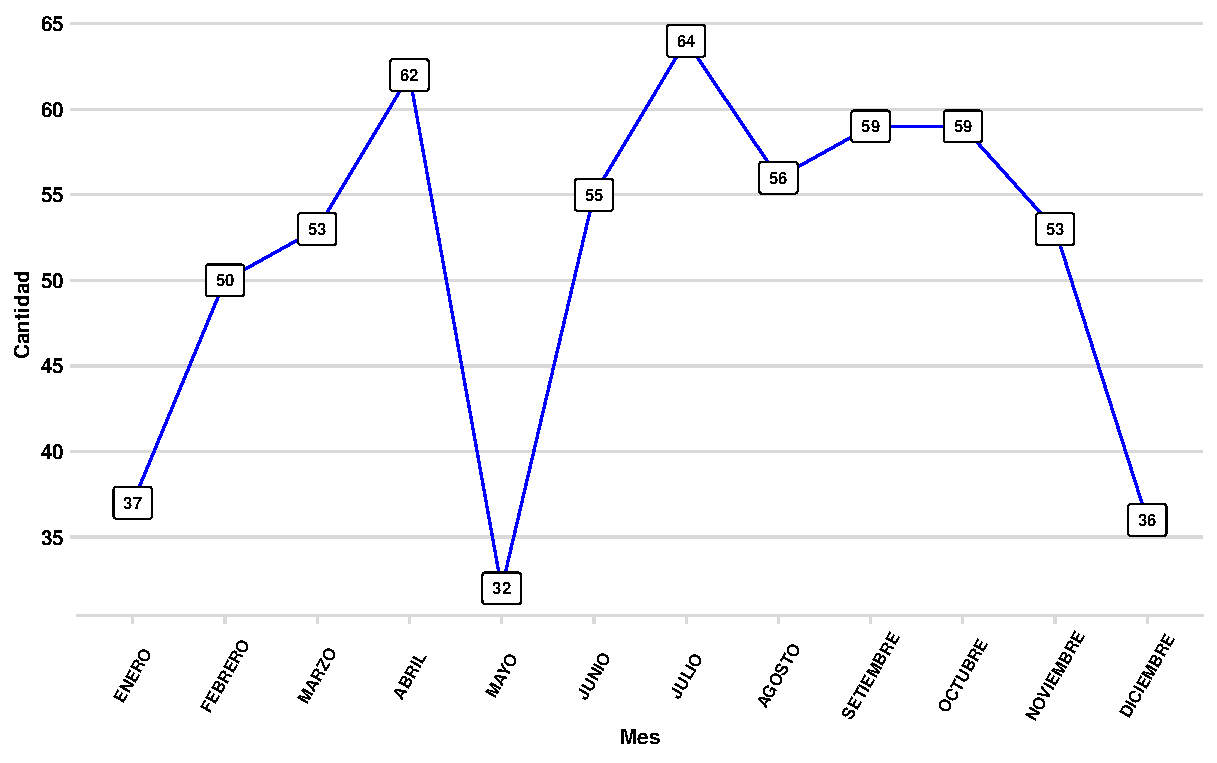
\includegraphics[width=15cm, height=5.95cm]{images/PROD005_demanda.pdf}}
  \label{fig:PROD005_demanda}
\end{figure}

La Figura \ref{fig:PROD005_demanda} muestra el diagrama de lineas que representa la evolución de la demanda de AJL VISC 1.4$\%$ - pack solución viscoelástica para uso intraocular hialuronato sódico 14 mg/ml canula 1x27g por mes en el año 2024, se observa que la demanda tiene un comportamiento determinístico a través de los meses del año, a excepción del mes de enero, mayo y diciembre en donde hubo puntos extremos, asimismo no se observa una tendencia y solo estacionariedad en el tiempo, por lo que tomando estos casos y el comportamiento de la demanda es necesario utilizar un \textsl{modelo determinístico EOQ}.

Tomando en cuenta la demanda total anual de la Tabla \ref{table:GrupoA_Area}, el costo de compra de la Tabla \ref{table:GrupoA_Costo_Compra}, el costo de preparación estimado de la Tabla \ref{table:GrupoA_Costo_Preparacion}, el costo de retención estimado de la Tabla \ref{table:GrupoA_Costo_Retencion} y tiempo de reabastecimiento del pedido brindado por el área de logística se tienen los siguientes valores:

\begin{itemize}
    \item \textbf{Demanda ($D$):} 616 unidades
    \item \textbf{Costo de compra ($C$):} S/ 90.00 por unidad
    \item \textbf{Costo de preparación ($K$):} S/ 7.70
    \item \textbf{Costo de retención ($h$):} S/ 11.23
    \item \textbf{Tiempo de entrega ($L$):} 7 días
\end{itemize}

Hallamos la cantidad de pedido óptima $y^*$ mediante la expresión (\ref{yopt}) de la siguiente manera
\begin{eqnarray}
    y^* &=& \sqrt{\frac{2KD}{h}} \nonumber \\
    y^* &=& \sqrt{\frac{2(7.7)(616)}{11.23}} \nonumber \\
    y^* &=& 29.06 \nonumber \\
    y^* &\thickapprox& 29 \text{ unidades} \nonumber
\end{eqnarray}
De la misma forma hallemos el intervalo de pedido óptimo $T^*$ utilizando la expresión (\ref{Topt}) 
\begin{eqnarray}
    T^* &=& \sqrt{\frac{2K}{Dh}} \nonumber
\end{eqnarray}
\begin{eqnarray}
    T^* &=& \sqrt{\frac{2(7.7)}{(616)(11.23)}} \nonumber \\
    T^* &=& 0.0472 \nonumber
\end{eqnarray}
Asimismo tomemos la demanda por día laborable (52 semanas * 5 días/semana = 260 días laborables) de tal forma que vemos el momento de cuando pedir
\begin{eqnarray}
    T^* &=& 0.0472 (260 \text{ días laborables}) \nonumber \\   
    T^* &=& 12.27 \nonumber \\
    T^* &\thickapprox& 12 \text{ días laborables} \nonumber
\end{eqnarray}
Ahora hallemos el costo mínimo total de inventario óptimo $CTI(y^*)$ usando la expresión (\ref{CTIopt}).
\begin{eqnarray}
    CTI(y^*) &=& \sqrt{2hKD} + DC \nonumber \\
    CTI(y^*) &=& \sqrt{2(11.23)(7.7)(616)} + (616)(90) \nonumber \\
    CTI(y^*) &=& \text{S/ 55,766.39} \nonumber
\end{eqnarray}
Por último hallemos el punto de reorden en base a la cantidad de pedido óptima y el tiempo de reabastecimiento de 7 días.
\begin{eqnarray}
    R &=& L_e D \nonumber \\
    R &=& (7) \left(\frac{616}{260 \text{ días laborables}} \right) \nonumber \\
    R &=& 16.58 \nonumber \\
    R &\thickapprox& 17 \text{ unidades} \nonumber
\end{eqnarray}

Esto quiere decir que cuando el inventario del producto llegue a 17 unidades se deben de realizar el pedido de 29 unidades, del cual el tiempo de pedido debería ser cada 12 días laborables teniendo un costo total de S/ 55,766.39
\clearpage
\subsubsection{Cuchillo lateral CLEAR CUT doble bisel 1.2 mm angulado}

El producto cuchillo lateral CLEAR CUT doble bisel 1.2 mm angulado de insumos generales del área de oftalmología es utilizado para las cirugía de facoemulsificación y extracción manual de catarata con incisión pequeña que son las cirugías para la extracción de catarata, primeramente observemos la tendencia de la demanda a lo largo del año 2024 en el siguiente gráfico.

\begin{figure}[H]
  \caption{Evolución demanda: Cuchillo lateral CLEAR CUT doble bisel 1.2 mm angulado de insumos generales - oftalmología}
  {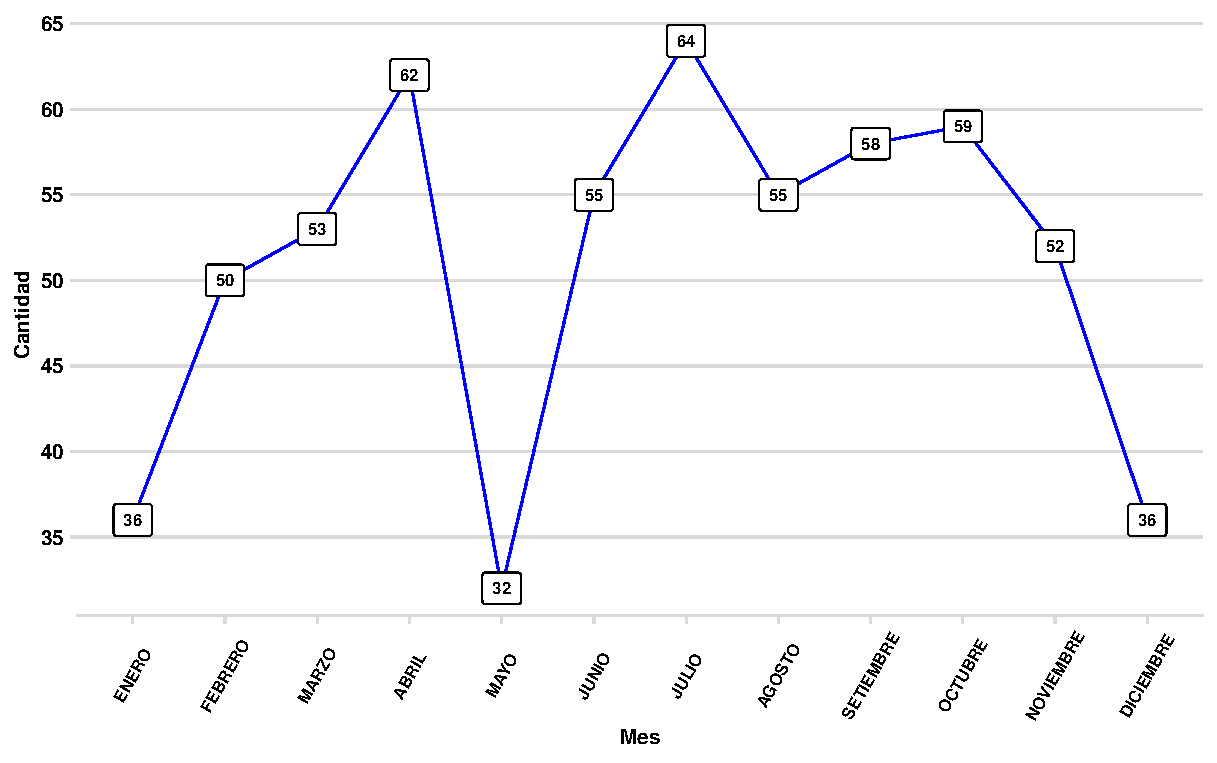
\includegraphics[width=15cm, height=5.95cm]{images/PROD006_demanda.pdf}}
  \label{fig:PROD006_demanda}
\end{figure}

La Figura \ref{fig:PROD006_demanda} muestra el diagrama de lineas que representa la evolución de la demanda del cuchillo lateral CLEAR CUT doble bisel 1.2 mm angulado por mes en el año 2024, se observa que la demanda tiene un comportamiento determinístico a través de los meses del año, a excepción del mes de enero, mayo y diciembre en donde hubo puntos extremos, asimismo no se observa una tendencia y solo estacionariedad en el tiempo, por lo que tomando estos casos y el comportamiento de la demanda es necesario utilizar un \textsl{modelo determinístico EOQ}.

Tomando en cuenta la demanda total anual de la Tabla \ref{table:GrupoA_Area}, el costo de compra de la Tabla \ref{table:GrupoA_Costo_Compra}, el costo de preparación estimado de la Tabla \ref{table:GrupoA_Costo_Preparacion}, el costo de retención estimado de la Tabla \ref{table:GrupoA_Costo_Retencion} y tiempo de reabastecimiento del pedido brindado por el área de logística se tienen los siguientes valores:

\begin{itemize}
    \item \textbf{Demanda ($D$):} 612 unidades
    \item \textbf{Costo de compra ($C$):} S/ 72.81 por unidad
    \item \textbf{Costo de preparación ($K$):} S/ 3.80
    \item \textbf{Costo de retención ($h$):} S/ 11.50
    \item \textbf{Tiempo de entrega ($L$):} 3 días
\end{itemize}

Hallamos la cantidad de pedido óptima $y^*$ mediante la expresión (\ref{yopt}) de la siguiente manera
\begin{eqnarray}
    y^* &=& \sqrt{\frac{2KD}{h}} \nonumber \\
    y^* &=& \sqrt{\frac{2(3.8)(612)}{11.5}} \nonumber \\
    y^* &=& 20.11 \nonumber \\
    y^* &\thickapprox& 20 \text{ unidades} \nonumber
\end{eqnarray}
De la misma forma hallemos el intervalo de pedido óptimo $T^*$ utilizando la expresión (\ref{Topt}) 
\begin{eqnarray}
    T^* &=& \sqrt{\frac{2K}{Dh}} \nonumber \\
    T^* &=& \sqrt{\frac{2(3.8)}{(612)(11.5)}} \nonumber \\
    T^* &=& 0.0329 \nonumber
\end{eqnarray}
Asimismo tomemos la demanda por día laborable (52 semanas * 5 días/semana = 260 días laborables) de tal forma que vemos el momento de cuando pedir
\begin{eqnarray}
    T^* &=& 0.0329 (260 \text{ días laborables}) \nonumber \\   
    T^* &=& 8.54 \nonumber \\
    T^* &\thickapprox& 9 \text{ días laborables} \nonumber
\end{eqnarray}
Ahora hallemos el costo mínimo total de inventario óptimo $CTI(y^*)$ usando la expresión (\ref{CTIopt}).
\begin{eqnarray}
    CTI(y^*) &=& \sqrt{2hKD} + DC \nonumber
\end{eqnarray}
\begin{eqnarray}
    CTI(y^*) &=& \sqrt{2(11.5)(3.8)(612)} + (612)(72.81) \nonumber \\
    CTI(y^*) &=& \text{S/ 44,791.00} \nonumber
\end{eqnarray}
Por último hallemos el punto de reorden en base a la cantidad de pedido óptima y el tiempo de reabastecimiento de 3 días.
\begin{eqnarray}
    R &=& L_e D \nonumber \\
    R &=& (3) \left(\frac{612}{260 \text{ días laborables}} \right) \nonumber \\
    R &=& 7.06 \nonumber \\
    R &\thickapprox& 7 \text{ unidades} \nonumber
\end{eqnarray}

Esto quiere decir que cuando el inventario del producto llegue a 7 unidades se deben de realizar el pedido de 20 unidades, del cual el tiempo de pedido debería ser cada 9 días laborables teniendo un costo total de S/ 44,791.00
\subsubsection{Solución de riboflavina VIBEX RAPID 0.1$\%$ isotonico jeringa de 1.5 ml}

El producto solución de riboflavina VIBEX RAPID 0.1$\%$ isotonico jeringa de 1.5 ml de CROSSLINKING del área de oftalmología es utilizado para las cirugías de queratocono, primeramente observemos la tendencia de la demanda a lo largo del año 2024 en el siguiente gráfico.

\begin{figure}[H]
  \caption{Evolución demanda: Solución de riboflavina VIBEX RAPID 0.1$\%$ de CROSSLINKING - oftalmología}
  {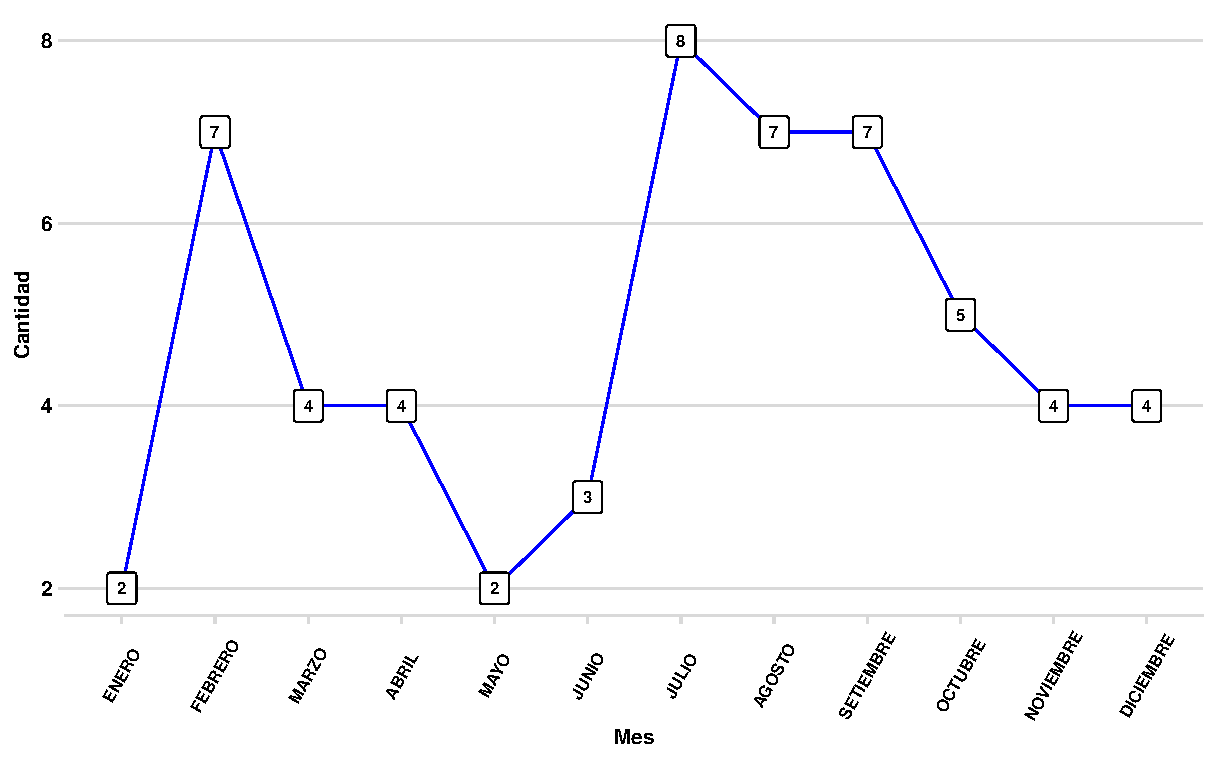
\includegraphics[width=15cm, height=5.85cm]{images/PROD007_demanda.pdf}}
  \label{fig:PROD007_demanda}
\end{figure}

La Figura \ref{fig:PROD007_demanda} muestra el diagrama de lineas que representa la evolución de la demanda de la solución de riboflavina VIBEX RAPID 0.1$\%$ por mes en el año 2024, se observa que la demanda tiene un comportamiento determinístico y estacionario sin tendencia a través de los meses del año, por lo que tomando estos casos y el comportamiento de la demanda es necesario utilizar un \textsl{modelo determinístico EOQ}.

Tomando en cuenta la demanda total anual de la Tabla \ref{table:GrupoA_Area}, el costo de compra de la Tabla \ref{table:GrupoA_Costo_Compra}, el costo de preparación estimado de la Tabla \ref{table:GrupoA_Costo_Preparacion}, el costo de retención estimado de la Tabla \ref{table:GrupoA_Costo_Retencion} y tiempo de reabastecimiento del pedido brindado por el área de logística se tienen los siguientes valores:

\begin{itemize}
    \item \textbf{Demanda ($D$):} 57 unidades
    \item \textbf{Costo de compra ($C$):} S/ 362.94 por unidad
    \item \textbf{Costo de preparación ($K$):} S/ 1.90
    \item \textbf{Costo de retención ($h$):} S/ 6.42
    \item \textbf{Tiempo de entrega ($L$):} 7 días
\end{itemize}

Hallamos la cantidad de pedido óptima $y^*$ mediante la expresión (\ref{yopt}) de la siguiente manera
\begin{eqnarray}
    y^* &=& \sqrt{\frac{2KD}{h}} \nonumber \\
    y^* &=& \sqrt{\frac{2(1.9)(57)}{6.42}} \nonumber \\
    y^* &=& 5.81 \nonumber \\
    y^* &\thickapprox& 6 \text{ unidades} \nonumber
\end{eqnarray}
De la misma forma hallemos el intervalo de pedido óptimo $T^*$ utilizando la expresión (\ref{Topt}) 
\begin{eqnarray}
    T^* &=& \sqrt{\frac{2K}{Dh}} \nonumber \\
    T^* &=& \sqrt{\frac{2(1.9)}{(57)(6.42)}} \nonumber \\
    T^* &=& 0.1019 \nonumber
\end{eqnarray}
Asimismo tomemos la demanda por día laborable (52 semanas * 5 días/semana = 260 días laborables) de tal forma que vemos el momento de cuando pedir
\begin{eqnarray}
    T^* &=& 0.1019 (260 \text{ días laborables}) \nonumber \\   
    T^* &=& 26.49 \nonumber \\
    T^* &\thickapprox& 26 \text{ días laborables} \nonumber
\end{eqnarray}
Ahora hallemos el costo mínimo total de inventario óptimo $CTI(y^*)$ usando la expresión (\ref{CTIopt}).
\begin{eqnarray}
    CTI(y^*) &=& \sqrt{2hKD} + DC \nonumber \\
    CTI(y^*) &=& \sqrt{2(6.42)(1.9)(57)} + (57)(362.94) \nonumber \\
    CTI(y^*) &=& \text{S/ 20,724.87} \nonumber
\end{eqnarray}
Por último hallemos el punto de reorden en base a la cantidad de pedido óptima y el tiempo de reabastecimiento de 7 días.
\begin{eqnarray}
    R &=& L_e D \nonumber \\
    R &=& (7) \left(\frac{57}{260 \text{ días laborables}} \right) \nonumber \\
    R &=& 1.53 \nonumber \\
    R &\thickapprox& 2 \text{ unidades} \nonumber
\end{eqnarray}

Esto quiere decir que cuando el inventario del producto llegue a 2 unidades se deben de realizar el pedido de 6 unidades, del cual el tiempo de pedido debería ser cada 26 días laborables teniendo un costo total de S/ 20,724.87
\subsubsection{Anterior chamber cannula 27g x 9mm BEND}

El producto anterior chamber cannula 27g x 9mm BEND de INLASER del área de oftalmología es utilizado para las cirugías refractivas LASIK, Presbyond y retoques LASIK realizados, observemos la tendencia de la demanda a lo largo del año 2024 en el siguiente gráfico.

\begin{figure}[H]
  \caption{Evolución demanda: Anterior chamber cannula 27g x 9mm BEND de INLASER - oftalmología}
  {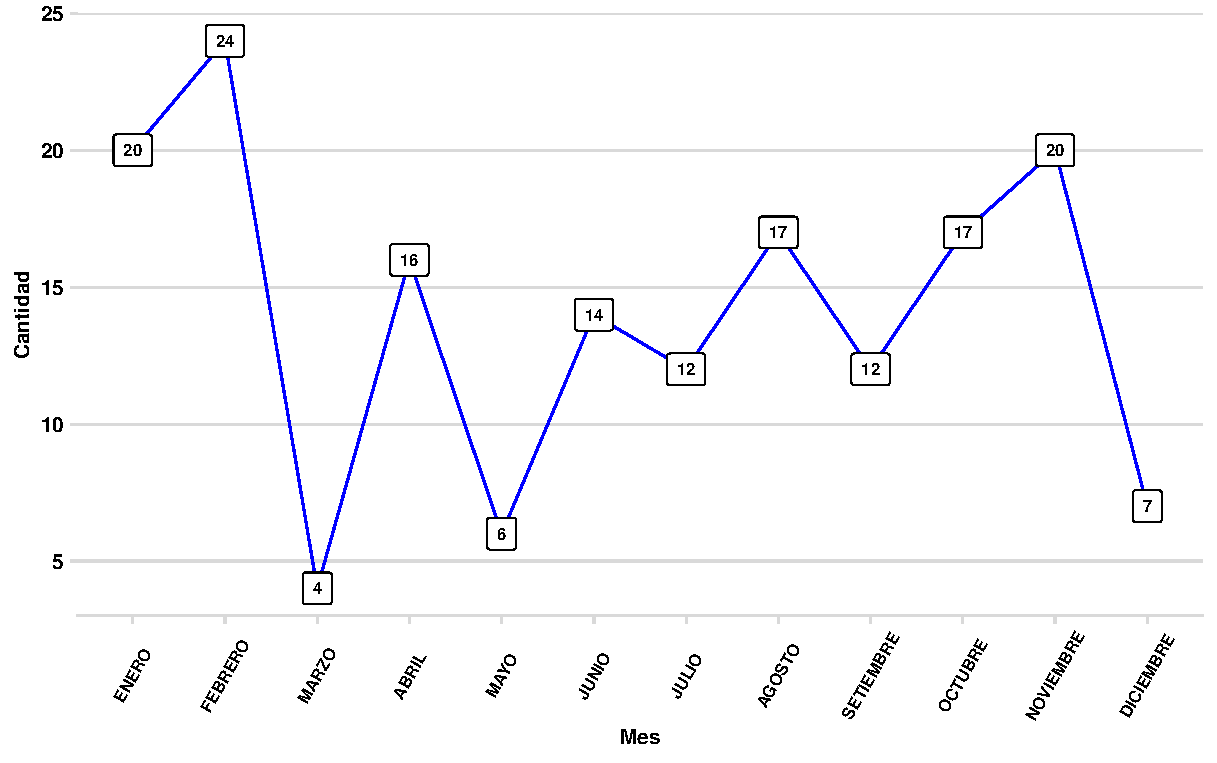
\includegraphics[width=15cm, height=5.95cm]{images/PROD008_demanda.pdf}}
  \label{fig:PROD008_demanda}
\end{figure}

La Figura \ref{fig:PROD008_demanda} muestra el diagrama de lineas que representa la evolución de la demanda del anterior chamber cannula 27g x 9mm BEND por mes en el año 2024, se observa que la demanda tiene un comportamiento determinístico y estacionario sin tendencia a través de los meses del año, por lo que tomando estos casos y el comportamiento de la demanda es necesario utilizar un \textsl{modelo determinístico EOQ}.

Tomando en cuenta la demanda total anual de la Tabla \ref{table:GrupoA_Area}, el costo de compra de la Tabla \ref{table:GrupoA_Costo_Compra}, el costo de preparación estimado de la Tabla \ref{table:GrupoA_Costo_Preparacion}, el costo de retención estimado de la Tabla \ref{table:GrupoA_Costo_Retencion} y tiempo de reabastecimiento del pedido brindado por el área de logística se tienen los siguientes valores:

\begin{itemize}
    \item \textbf{Demanda ($D$):} 169 unidades
    \item \textbf{Costo de compra ($C$):} S/ 16.00 por unidad
    \item \textbf{Costo de preparación ($K$):} S/ 7.70
    \item \textbf{Costo de retención ($h$):} S/ 12.30
    \item \textbf{Tiempo de entrega ($L$):} 7 días
\end{itemize}
Hallamos la cantidad de pedido óptima $y^*$ mediante la expresión (\ref{yopt}) de la siguiente manera
\begin{eqnarray}
    y^* &=& \sqrt{\frac{2KD}{h}} \nonumber
\end{eqnarray}
\begin{eqnarray}
    y^* &=& \sqrt{\frac{2(7.7)(169)}{12.3}} \nonumber \\
    y^* &=& 14.55 \nonumber \\
    y^* &\thickapprox& 15 \text{ unidades} \nonumber
\end{eqnarray}
De la misma forma hallemos el intervalo de pedido óptimo $T^*$ utilizando la expresión (\ref{Topt}) 
\begin{eqnarray}
    T^* &=& \sqrt{\frac{2K}{Dh}} \nonumber \\
    T^* &=& \sqrt{\frac{2(7.7)}{(169)(12.3)}} \nonumber \\
    T^* &=& 0.0861 \nonumber
\end{eqnarray}
Asimismo tomemos la demanda por día laborable (52 semanas * 5 días/semana = 260 días laborables) de tal forma que vemos el momento de cuando pedir
\begin{eqnarray}
    T^* &=& 0.0861 (260 \text{ días laborables}) \nonumber \\   
    T^* &=& 22.38 \nonumber \\
    T^* &\thickapprox& 22 \text{ días laborables} \nonumber
\end{eqnarray}
Ahora hallemos el costo mínimo total de inventario óptimo $CTI(y^*)$ usando la expresión (\ref{CTIopt}).
\begin{eqnarray}
    CTI(y^*) &=& \sqrt{2hKD} + DC \nonumber \\
    CTI(y^*) &=& \sqrt{2(12.3)(7.7)(169)} + (169)(16) \nonumber \\
    CTI(y^*) &=& \text{S/ 2,882.92} \nonumber
\end{eqnarray}
Por último hallemos el punto de reorden en base a la cantidad de pedido óptima y el tiempo de reabastecimiento de 7 días.
\begin{eqnarray}
    R &=& L_e D \nonumber \\
    R &=& (7) \left(\frac{169}{260 \text{ días laborables}} \right) \nonumber
\end{eqnarray}
\begin{eqnarray}
    R &=& 4.55 \nonumber \\
    R &\thickapprox& 5 \text{ unidades} \nonumber
\end{eqnarray}

Esto quiere decir que cuando el inventario del producto llegue a 5 unidades se deben de realizar el pedido de 15 unidades, del cual el tiempo de pedido debería ser cada 22 días laborables teniendo un costo total de S/ 2,882.92
\subsubsection{Canula para cistotoma formada 27g}

El producto canula para cistotoma formada 27g de FACO del área de oftalmología es utilizado para la cirugía de facoemulsificación y extracción manual de catarata con incisión pequeña que son las cirugías para la extracción de catarata, primeramente observemos la tendencia de la demanda a lo largo del año 2024 en el siguiente gráfico.

\begin{figure}[H]
  \caption{Evolución demanda: canula para cistotoma formada 27g de FACO - oftalmología}
  {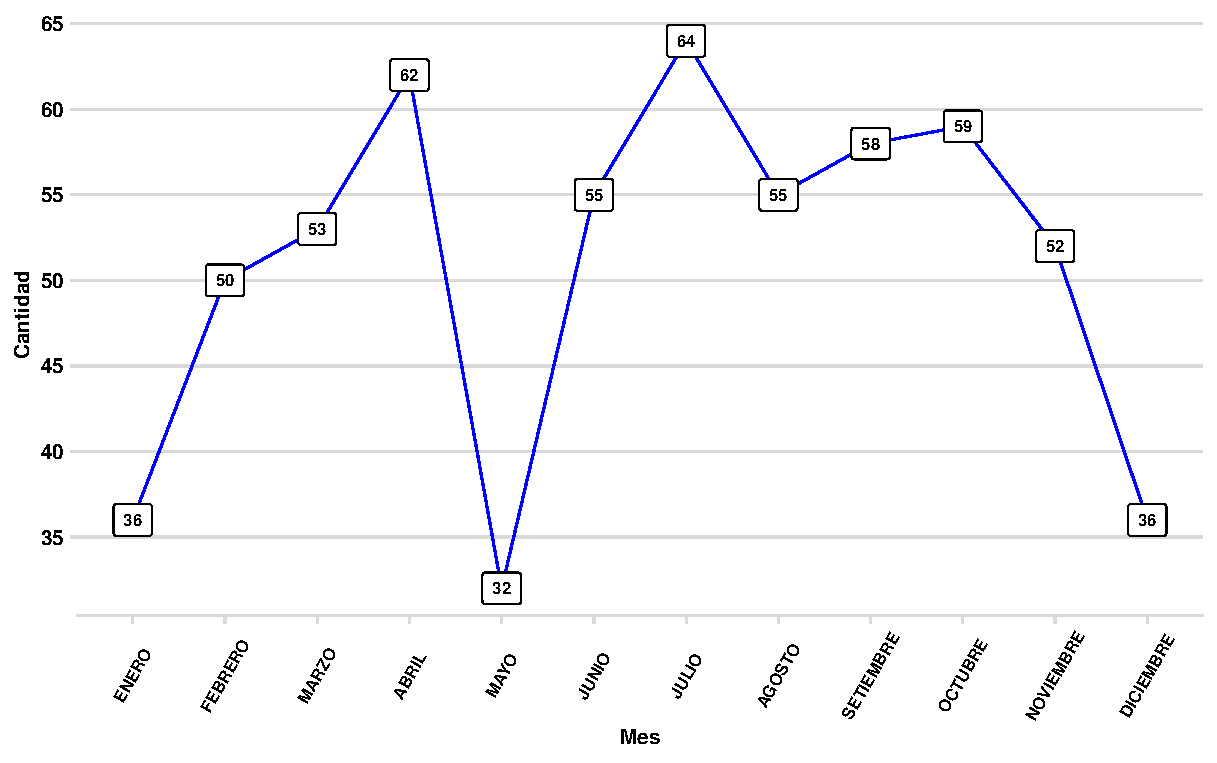
\includegraphics[width=15cm, height=5.95cm]{images/PROD009_demanda.pdf}}
  \label{fig:PROD009_demanda}
\end{figure}

La Figura \ref{fig:PROD009_demanda} muestra el diagrama de lineas que representa la evolución de la demanda de la canula para cistotoma formada 27g por mes en el año 2024, se observa que la demanda tiene un comportamiento determinístico y estacionario sin tendencia a través de los meses del año, por lo que tomando estos casos y el comportamiento de la demanda es necesario utilizar un \textsl{modelo determinístico EOQ}.

Tomando en cuenta la demanda total anual de la Tabla \ref{table:GrupoA_Area}, el costo de compra de la Tabla \ref{table:GrupoA_Costo_Compra}, el costo de preparación estimado de la Tabla \ref{table:GrupoA_Costo_Preparacion}, el costo de retención estimado de la Tabla \ref{table:GrupoA_Costo_Retencion} y tiempo de reabastecimiento del pedido brindado por el área de logística se tienen los siguientes valores:

\begin{itemize}
    \item \textbf{Demanda ($D$):} 612 unidades
    \item \textbf{Costo de compra ($C$):} S/ 143.00 por unidad
    \item \textbf{Costo de preparación ($K$):} S/ 9.61
    \item \textbf{Costo de retención ($h$):} S/ 8.56
    \item \textbf{Tiempo de entrega ($L$):} 7 días
\end{itemize}

Hallamos la cantidad de pedido óptima $y^*$ mediante la expresión (\ref{yopt}) de la siguiente manera
\begin{eqnarray}
    y^* &=& \sqrt{\frac{2KD}{h}} \nonumber \\
    y^* &=& \sqrt{\frac{2(9.61)(612)}{8.56}} \nonumber \\
    y^* &=& 37.07 \nonumber \\
    y^* &\thickapprox& 37 \text{ unidades} \nonumber
\end{eqnarray}
De la misma forma hallemos el intervalo de pedido óptimo $T^*$ utilizando la expresión (\ref{Topt}) 
\begin{eqnarray}
    T^* &=& \sqrt{\frac{2K}{Dh}} \nonumber \\
    T^* &=& \sqrt{\frac{2(9.61)}{(612)(8.56)}} \nonumber \\
    T^* &=& 0.0606 \nonumber
\end{eqnarray}
Asimismo tomemos la demanda por día laborable (52 semanas * 5 días/semana = 260 días laborables) de tal forma que vemos el momento de cuando pedir
\begin{eqnarray}
    T^* &=& 0.0606 (260 \text{ días laborables}) \nonumber \\   
    T^* &=& 15.75 \nonumber \\
    T^* &\thickapprox& 16 \text{ días laborables} \nonumber
\end{eqnarray}
Ahora hallemos el costo mínimo total de inventario óptimo $CTI(y^*)$ usando la expresión (\ref{CTIopt}).
\begin{eqnarray}
    CTI(y^*) &=& \sqrt{2hKD} + DC \nonumber \\
    CTI(y^*) &=& \sqrt{2(8.56)(9.61)(612)} + (612)(143) \nonumber \\
    CTI(y^*) &=& \text{S/ 87,833.31} \nonumber
\end{eqnarray}
Por último hallemos el punto de reorden en base a la cantidad de pedido óptima y el tiempo de reabastecimiento de 7 días.
\begin{eqnarray}
    R &=& L_e D \nonumber \\
    R &=& (7) \left(\frac{612}{260 \text{ días laborables}} \right) \nonumber \\
    R &=& 16.48 \nonumber \\
    R &\thickapprox& 16 \text{ unidades} \nonumber
\end{eqnarray}

Esto quiere decir que cuando el inventario del producto llegue a 16 unidades se deben de realizar el pedido de 37 unidades, del cual el tiempo de pedido debería ser cada 16 días laborables teniendo un costo total de S/ 87,833.31
\subsubsection{Toner TNP80Y yellow para Konica Minolta BIZHUB C-3320i}
El producto toner TNP80Y yellow para Konica Minolta de Tintas del área de oftalmología es utilizado para las impresiones realizadas en el área de exámenes especiales en tomografías realizadas, primeramente observemos la tendencia de la demanda a lo largo del año 2024 en el siguiente gráfico.
\clearpage
\begin{figure}[H]
  \caption{Evolución demanda: Toner TNP80Y yellow para Konica Minolta de Tintas - oftalmología}
  {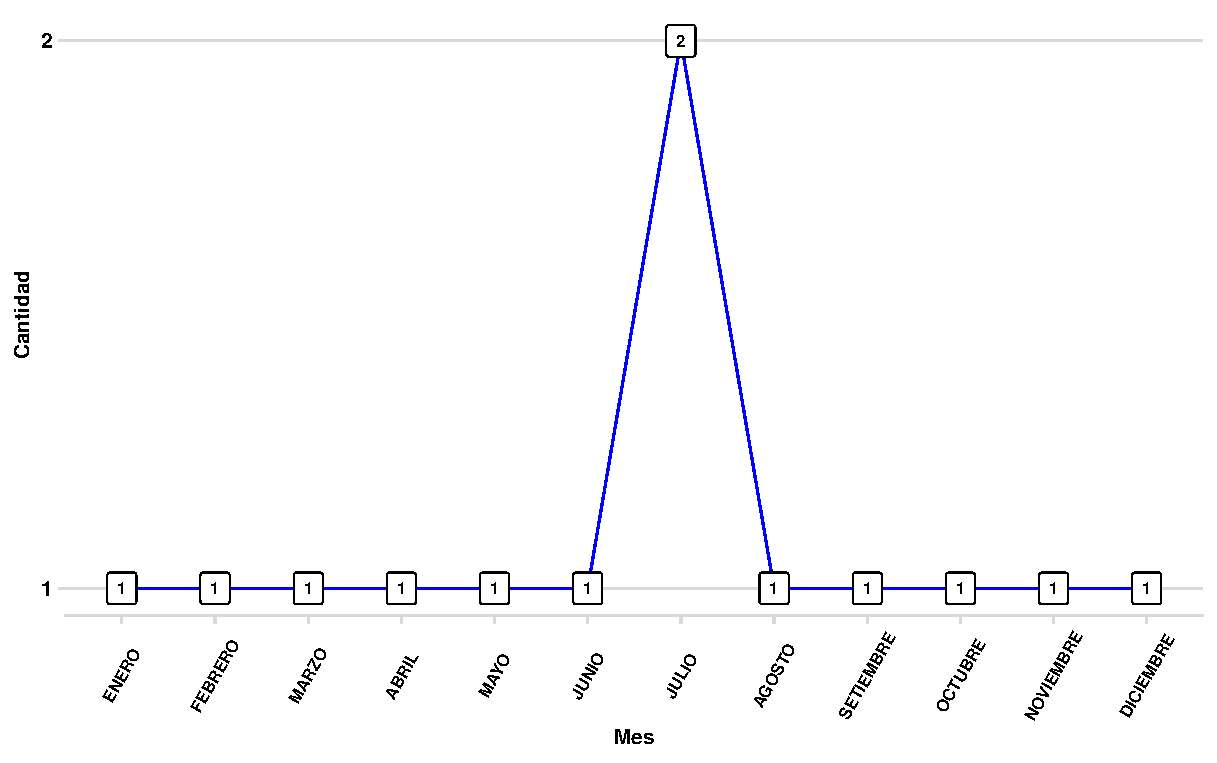
\includegraphics[width=15cm, height=5.95cm]{images/PROD010_demanda.pdf}}
  \label{fig:PROD010_demanda}
\end{figure}

La Figura \ref{fig:PROD010_demanda} muestra el diagrama de lineas que representa la evolución de la demanda del toner TNP80Y yellow por mes en el año 2024, se observa que la demanda tiene un comportamiento determinístico y sin estacionariedad ya que parece constante en los meses sin tendencia, tomando estos casos y el comportamiento de la demanda es necesario utilizar un \textsl{modelo determinístico EOQ}.

Tomando en cuenta la demanda total anual de la Tabla \ref{table:GrupoA_Area}, el costo de compra de la Tabla \ref{table:GrupoA_Costo_Compra}, el costo de preparación estimado de la Tabla \ref{table:GrupoA_Costo_Preparacion}, el costo de retención estimado de la Tabla \ref{table:GrupoA_Costo_Retencion} y tiempo de reabastecimiento del pedido brindado por el área de logística se tienen los siguientes valores:

\begin{itemize}
    \item \textbf{Demanda ($D$):} 13 unidades
    \item \textbf{Costo de compra ($C$):} S/ 720.00 por unidad
    \item \textbf{Costo de preparación ($K$):} S/ 11.51
    \item \textbf{Costo de retención ($h$):} S/ 7.76
    \item \textbf{Tiempo de entrega ($L$):} 1 día
\end{itemize}

Hallamos la cantidad de pedido óptima $y^*$ mediante la expresión (\ref{yopt}) de la siguiente manera
\begin{eqnarray}
    y^* &=& \sqrt{\frac{2KD}{h}} \nonumber
\end{eqnarray}
\begin{eqnarray}
    y^* &=& \sqrt{\frac{2(11.51)(13)}{7.76}} \nonumber \\
    y^* &=& 6.21 \nonumber \\
    y^* &\thickapprox& 6 \text{ unidades} \nonumber
\end{eqnarray}
De la misma forma hallemos el intervalo de pedido óptimo $T^*$ utilizando la expresión (\ref{Topt}) 
\begin{eqnarray}
    T^* &=& \sqrt{\frac{2K}{Dh}} \nonumber \\
    T^* &=& \sqrt{\frac{2(11.51)}{(13)(7.76)}} \nonumber \\
    T^* &=& 0.4777 \nonumber
\end{eqnarray}
Asimismo tomemos la demanda por día laborable (52 semanas * 5 días/semana = 260 días laborables) de tal forma que vemos el momento de cuando pedir
\begin{eqnarray}
    T^* &=& 0.4777 (260 \text{ días laborables}) \nonumber \\   
    T^* &=& 124.2 \nonumber \\
    T^* &\thickapprox& 124 \text{ días laborables} \nonumber
\end{eqnarray}
Ahora hallemos el costo mínimo total de inventario óptimo $CTI(y^*)$ usando la expresión (\ref{CTIopt}).
\begin{eqnarray}
    CTI(y^*) &=& \sqrt{2hKD} + DC \nonumber \\
    CTI(y^*) &=& \sqrt{2(7.76)(11.51)(13)} + (13)(720) \nonumber \\
    CTI(y^*) &=& \text{S/ 9,408.19} \nonumber
\end{eqnarray}
Por último hallemos el punto de reorden en base a la cantidad de pedido óptima y el tiempo de reabastecimiento de 1 día.
\begin{eqnarray}
    R &=& L_e D \nonumber \\
    R &=& (1) \left(\frac{13}{260 \text{ días laborables}} \right) \nonumber
\end{eqnarray}
\begin{eqnarray}
    R &=& 0.05 \nonumber \\
    R &\thickapprox& 0 \text{ unidades} \nonumber
\end{eqnarray}

Esto quiere decir que cuando el inventario del producto llegue a 0 unidades se deben de realizar el pedido de 6 unidades, del cual el tiempo de pedido debería ser cada 124 días laborables teniendo un costo total de S/ 9,408.19
\subsubsection{Campo quirúrgico para ojos desechable 100 cm x 70 cm}
El producto campo quirúrgico para ojos desechable 100 cm x 70 cm de Insumos generales del área de oftalmología es utilizado para las cirugías oftalmológicas realizadas en general, primeramente observemos la tendencia de la demanda a lo largo del año 2024 en el siguiente gráfico.

\begin{figure}[H]
  \caption{Evolución demanda: Campo quirúrgico para ojos desechable 100 cm x 70 cm de Insumos generales - oftalmología}
  {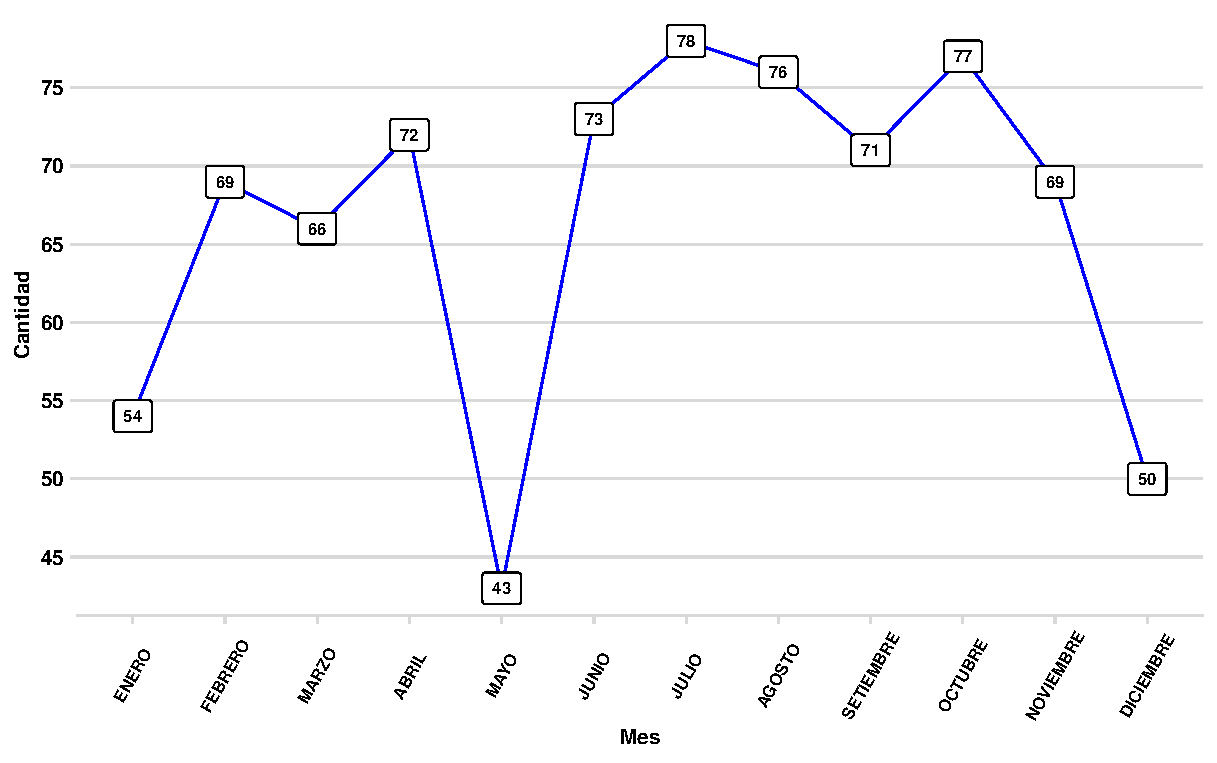
\includegraphics[width=15cm, height=5.95cm]{images/PROD011_demanda.pdf}}
  \label{fig:PROD011_demanda}
\end{figure}

La Figura \ref{fig:PROD011_demanda} muestra el diagrama de lineas que representa la evolución de la demanda del campo quirúrgico para ojos desechable 100 cm x 70 cm por mes en el año 2024, se observa que la demanda tiene un comportamiento determinístico a través de los meses del año, a excepción del mes de enero, mayo y diciembre en donde hubo puntos extremos bajos, asimismo no se observa una tendencia y solo estacionariedad en el tiempo, por lo que tomando estos casos y el comportamiento de la demanda es necesario utilizar un \textsl{modelo determinístico EOQ}.

Tomando en cuenta la demanda total anual de la Tabla \ref{table:GrupoA_Area}, el costo de compra de la Tabla \ref{table:GrupoA_Costo_Compra}, el costo de preparación estimado de la Tabla \ref{table:GrupoA_Costo_Preparacion}, el costo de retención estimado de la Tabla \ref{table:GrupoA_Costo_Retencion} y tiempo de reabastecimiento del pedido brindado por el área de logística se tienen los siguientes valores:

\begin{itemize}
    \item \textbf{Demanda ($D$):} 798 unidades
    \item \textbf{Costo de compra ($C$):} S/ 15.59 por unidad
    \item \textbf{Costo de preparación ($K$):} S/ 13.50
    \item \textbf{Costo de retención ($h$):} S/ 19.79
    \item \textbf{Tiempo de entrega ($L$):} 4 días
\end{itemize}

Hallamos la cantidad de pedido óptima $y^*$ mediante la expresión (\ref{yopt}) de la siguiente manera
\begin{eqnarray}
    y^* &=& \sqrt{\frac{2KD}{h}} \nonumber \\
    y^* &=& \sqrt{\frac{2(13.5)(798)}{19.79}} \nonumber \\
    y^* &=& 33.00 \nonumber \\
    y^* &\thickapprox& 33 \text{ unidades} \nonumber
\end{eqnarray}
De la misma forma hallemos el intervalo de pedido óptimo $T^*$ utilizando la expresión (\ref{Topt}) 
\begin{eqnarray}
    T^* &=& \sqrt{\frac{2K}{Dh}} \nonumber \\
    T^* &=& \sqrt{\frac{2(13.5)}{(798)(19.79)}} \nonumber \\
    T^* &=& 0.0413 \nonumber
\end{eqnarray}
Asimismo tomemos la demanda por día laborable (52 semanas * 5 días/semana = 260 días laborables) de tal forma que vemos el momento de cuando pedir
\begin{eqnarray}
    T^* &=& 0.0413 (260 \text{ días laborables}) \nonumber
\end{eqnarray}
\begin{eqnarray}
    T^* &=& 10.75 \nonumber \\
    T^* &\thickapprox& 11 \text{ días laborables} \nonumber
\end{eqnarray}
Ahora hallemos el costo mínimo total de inventario óptimo $CTI(y^*)$ usando la expresión (\ref{CTIopt}).
\begin{eqnarray}
    CTI(y^*) &=& \sqrt{2hKD} + DC \nonumber \\
    CTI(y^*) &=& \sqrt{2(19.79)(13.5)(798)} + (798)(15.59) \nonumber \\
    CTI(y^*) &=& \text{S/ 13,093.81} \nonumber
\end{eqnarray}
Por último hallemos el punto de reorden en base a la cantidad de pedido óptima y el tiempo de reabastecimiento de 4 días.
\begin{eqnarray}
    R &=& L_e D \nonumber \\
    R &=& (4) \left(\frac{798}{260 \text{ días laborables}} \right) \nonumber \\
    R &=& 12.28 \nonumber \\
    R &\thickapprox& 12 \text{ unidades} \nonumber
\end{eqnarray}

Esto quiere decir que cuando el inventario del producto llegue a 12 unidades se deben de realizar el pedido de 33 unidades, del cual el tiempo de pedido debería ser cada 11 días laborables teniendo un costo total de S/ 13,093.81
\subsubsection{Toner TNP80C cyan para Konica Minolta BIZHUB C-3320i}

El producto toner TNP80C cyan para Konica Minolta de Tintas del área de oftalmología es utilizado para las impresiones realizadas en el área de exámenes especiales en tomografías realizadas, primeramente observemos la tendencia de la demanda a lo largo del año 2024 en el siguiente gráfico.
\clearpage
\begin{figure}[H]
  \caption{Evolución demanda: Toner TNP80C cyan para Konica Minolta de Tintas - oftalmología}
  {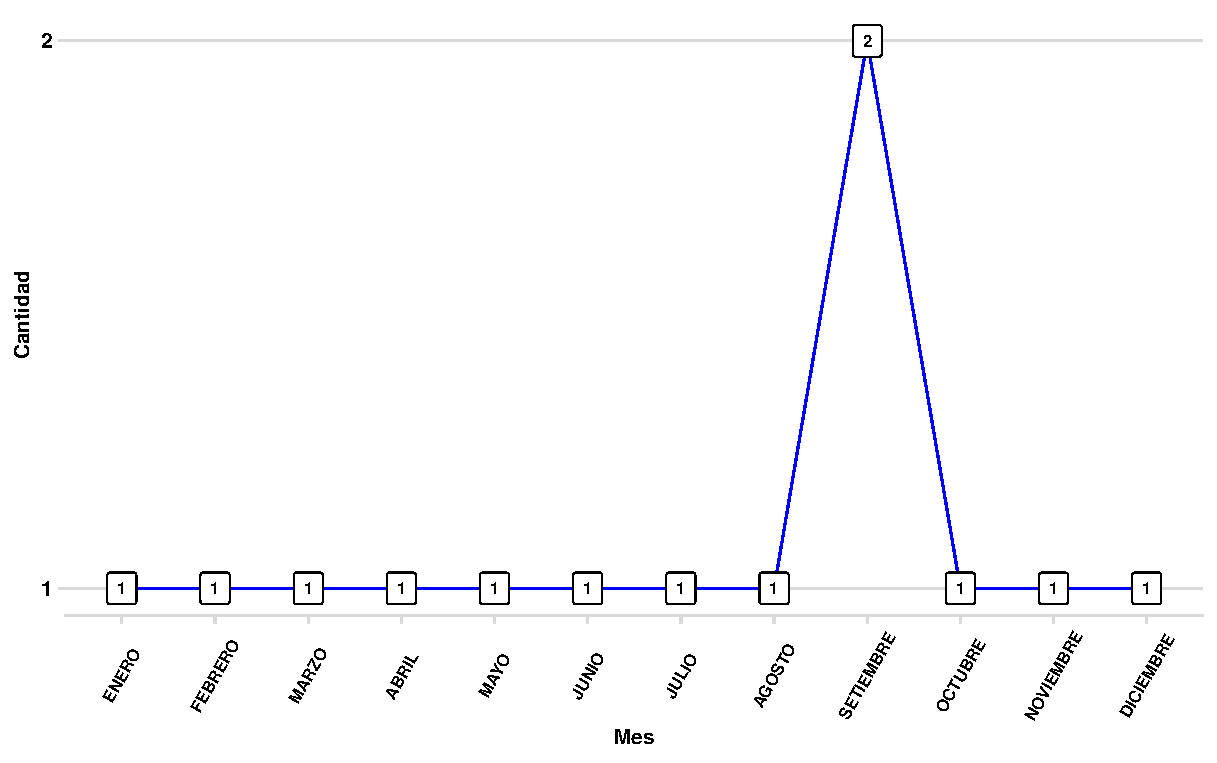
\includegraphics[width=15cm, height=5.95cm]{images/PROD012_demanda.pdf}}
  \label{fig:PROD012_demanda}
\end{figure}

La Figura \ref{fig:PROD012_demanda} muestra el diagrama de lineas que representa la evolución de la demanda del toner TNP80C cyan por mes en el año 2024, se observa que la demanda tiene un comportamiento determinístico y sin estacionariedad ya que parece constante en los meses sin tendencia, tomando estos casos y el comportamiento de la demanda es necesario utilizar un \textsl{modelo determinístico EOQ}.

Tomando en cuenta la demanda total anual de la Tabla \ref{table:GrupoA_Area}, el costo de compra de la Tabla \ref{table:GrupoA_Costo_Compra}, el costo de preparación estimado de la Tabla \ref{table:GrupoA_Costo_Preparacion}, el costo de retención estimado de la Tabla \ref{table:GrupoA_Costo_Retencion} y tiempo de reabastecimiento del pedido brindado por el área de logística se tienen los siguientes valores:

\begin{itemize}
    \item \textbf{Demanda ($D$):} 13 unidades
    \item \textbf{Costo de compra ($C$):} S/ 715.00 por unidad
    \item \textbf{Costo de preparación ($K$):} S/ 15.41
    \item \textbf{Costo de retención ($h$):} S/ 7.76
    \item \textbf{Tiempo de entrega ($L$):} 1 día
\end{itemize}

Hallamos la cantidad de pedido óptima $y^*$ mediante la expresión (\ref{yopt}) de la siguiente manera
\begin{eqnarray}
    y^* &=& \sqrt{\frac{2KD}{h}} \nonumber
\end{eqnarray}
\begin{eqnarray}
    y^* &=& \sqrt{\frac{2(15.41)(13)}{7.76}} \nonumber \\
    y^* &=& 7.19 \nonumber \\
    y^* &\thickapprox& 7 \text{ unidades} \nonumber
\end{eqnarray}
De la misma forma hallemos el intervalo de pedido óptimo $T^*$ utilizando la expresión (\ref{Topt}) 
\begin{eqnarray}
    T^* &=& \sqrt{\frac{2K}{Dh}} \nonumber \\
    T^* &=& \sqrt{\frac{2(15.41)}{(13)(7.76)}} \nonumber \\
    T^* &=& 0.5527 \nonumber
\end{eqnarray}
Asimismo tomemos la demanda por día laborable (52 semanas * 5 días/semana = 260 días laborables) de tal forma que vemos el momento de cuando pedir
\begin{eqnarray}
    T^* &=& 0.5527 (260 \text{ días laborables}) \nonumber \\   
    T^* &=& 143.71 \nonumber \\
    T^* &\thickapprox& 144 \text{ días laborables} \nonumber
\end{eqnarray}
Ahora hallemos el costo mínimo total de inventario óptimo $CTI(y^*)$ usando la expresión (\ref{CTIopt}).
\begin{eqnarray}
    CTI(y^*) &=& \sqrt{2hKD} + DC \nonumber \\
    CTI(y^*) &=& \sqrt{2(7.76)(15.41)(13)} + (13)(715) \nonumber \\
    CTI(y^*) &=& \text{S/ 9,350.76} \nonumber
\end{eqnarray}
Por último hallemos el punto de reorden en base a la cantidad de pedido óptima y el tiempo de reabastecimiento de 1 día.
\begin{eqnarray}
    R &=& L_e D \nonumber \\
    R &=& (1) \left(\frac{13}{260 \text{ días laborables}} \right) \nonumber
\end{eqnarray}
\begin{eqnarray}
    R &=& 0.05 \nonumber \\
    R &\thickapprox& 0 \text{ unidades} \nonumber
\end{eqnarray}

Esto quiere decir que cuando el inventario del producto llegue a 0 unidades se deben de realizar el pedido de 7 unidades, del cual el tiempo de pedido debería ser cada 144 días laborables teniendo un costo total de S/ 9,350.76
\subsubsection{Lentes de contacto - AIR optix día y noche}

El producto lentes de contacto - AIR optix día y noche de Insumos generales del área de oftalmología es utilizado generalmente en las cirugías de Pterigion usado para remover la carnosidad en la conjuntiva que llega a la córnea, también utilizado en algunas cirugías de catarata si es necesario, primeramente observemos la tendencia de la demanda a lo largo del año 2024 en el siguiente gráfico.

\begin{figure}[H]
  \caption{Evolución demanda: Lentes de contacto - AIR optix día y noche de Insumos generales - oftalmología}
  {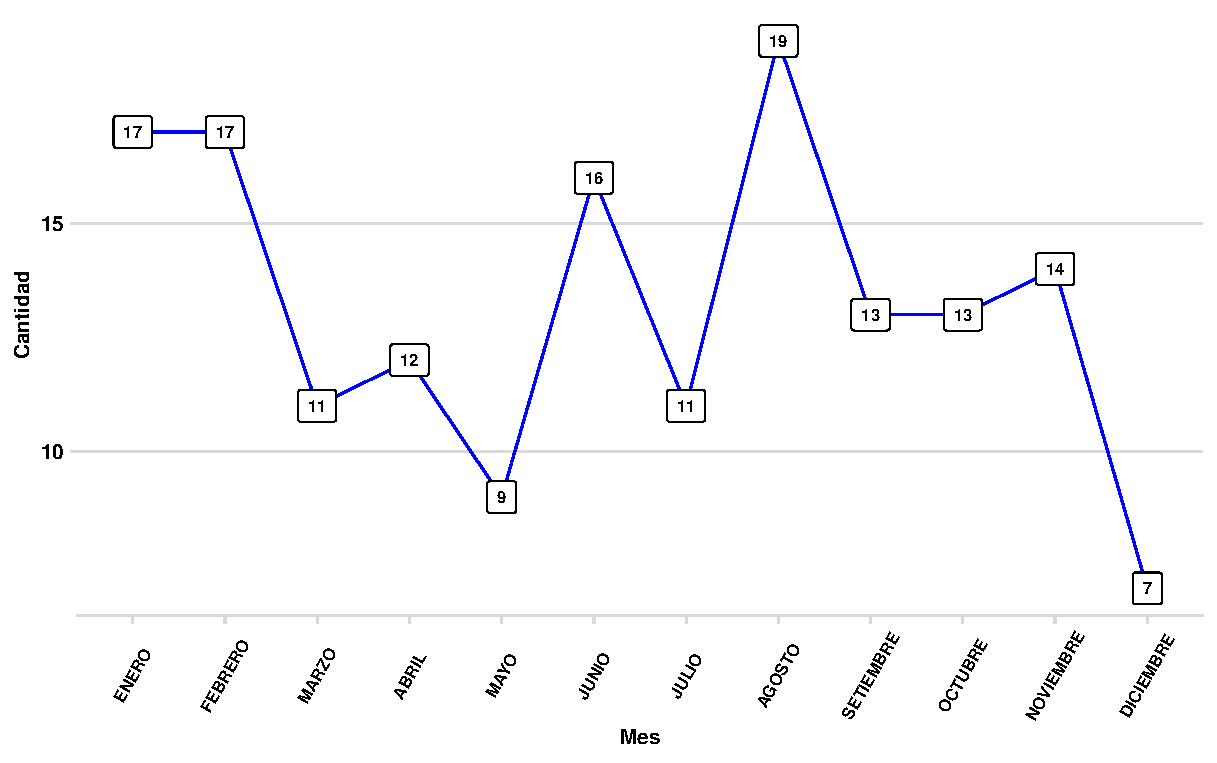
\includegraphics[width=15cm, height=5.95cm]{images/PROD013_demanda.pdf}}
  \label{fig:PROD013_demanda}
\end{figure}

La Figura \ref{fig:PROD013_demanda} muestra el diagrama de lineas que representa la evolución de la demanda del campo quirúrgico para ojos desechable 100 cm x 70 cm por mes en el año 2024, se observa que la demanda tiene un comportamiento determinístico a través de los meses del año, a excepción del mes de diciembre en donde se encuentra el valor más bajo, asimismo no se observa una tendencia y solo estacionariedad en el tiempo, por lo que tomando estos casos y el comportamiento de la demanda es necesario utilizar un \textsl{modelo determinístico EOQ}.

Tomando en cuenta la demanda total anual de la Tabla \ref{table:GrupoA_Area}, el costo de compra de la Tabla \ref{table:GrupoA_Costo_Compra}, el costo de preparación estimado de la Tabla \ref{table:GrupoA_Costo_Preparacion}, el costo de retención estimado de la Tabla \ref{table:GrupoA_Costo_Retencion} y tiempo de reabastecimiento del pedido brindado por el área de logística se tienen los siguientes valores:

\begin{itemize}
    \item \textbf{Demanda ($D$):} 159 unidades
    \item \textbf{Costo de compra ($C$):} S/ 143.37 por unidad
    \item \textbf{Costo de preparación ($K$):} S/ 1.90
    \item \textbf{Costo de retención ($h$):} S/ 6.42
    \item \textbf{Tiempo de entrega ($L$):} 3 días
\end{itemize}

Hallamos la cantidad de pedido óptima $y^*$ mediante la expresión (\ref{yopt}) de la siguiente manera
\begin{eqnarray}
    y^* &=& \sqrt{\frac{2KD}{h}} \nonumber \\
    y^* &=& \sqrt{\frac{2(1.9)(159)}{6.42}} \nonumber \\
    y^* &=& 9.7 \nonumber \\
    y^* &\thickapprox& 10 \text{ unidades} \nonumber
\end{eqnarray}
De la misma forma hallemos el intervalo de pedido óptimo $T^*$ utilizando la expresión (\ref{Topt}) 
\begin{eqnarray}
    T^* &=& \sqrt{\frac{2K}{Dh}} \nonumber \\
    T^* &=& \sqrt{\frac{2(1.9)}{(159)(6.42)}} \nonumber \\
    T^* &=& 0.0610 \nonumber
\end{eqnarray}
Asimismo tomemos la demanda por día laborable (52 semanas * 5 días/semana = 260 días laborables) de tal forma que vemos el momento de cuando pedir
\begin{eqnarray}
    T^* &=& 0.0610 (260 \text{ días laborables}) \nonumber
\end{eqnarray}
\begin{eqnarray}
    T^* &=& 15.86 \nonumber \\
    T^* &\thickapprox& 16 \text{ días laborables} \nonumber
\end{eqnarray}
Ahora hallemos el costo mínimo total de inventario óptimo $CTI(y^*)$ usando la expresión (\ref{CTIopt}).
\begin{eqnarray}
    CTI(y^*) &=& \sqrt{2hKD} + DC \nonumber \\
    CTI(y^*) &=& \sqrt{2(6.42)(1.9)(159)} + (159)(143.37) \nonumber \\
    CTI(y^*) &=& \text{S/ 22,858.11} \nonumber
\end{eqnarray}
Por último hallemos el punto de reorden en base a la cantidad de pedido óptima y el tiempo de reabastecimiento de 3 días.
\begin{eqnarray}
    R &=& L_e D \nonumber \\
    R &=& (3) \left(\frac{159}{260 \text{ días laborables}} \right) \nonumber \\
    R &=& 1.83 \nonumber \\
    R &\thickapprox& 2 \text{ unidades} \nonumber
\end{eqnarray}

Esto quiere decir que cuando el inventario del producto llegue a 2 unidades se deben de realizar el pedido de 10 unidades, del cual el tiempo de pedido debería ser cada 16 días laborables teniendo un costo total de S/ 22,858.11
\subsubsection{Toner Konica Minolta BIZHUB C-3320i Magenta}

El producto toner Konica Minolta BIZHUB C-3320i magenta de Tintas del área de oftalmología es utilizado para las impresiones realizadas en el área de exámenes especiales en tomografías realizadas, primeramente observemos la tendencia de la demanda a lo largo del año 2024 en el siguiente gráfico.
\clearpage
\begin{figure}[H]
  \caption{Evolución demanda: Toner Konica Minolta BIZHUB C-3320i de Tintas - oftalmología}
  {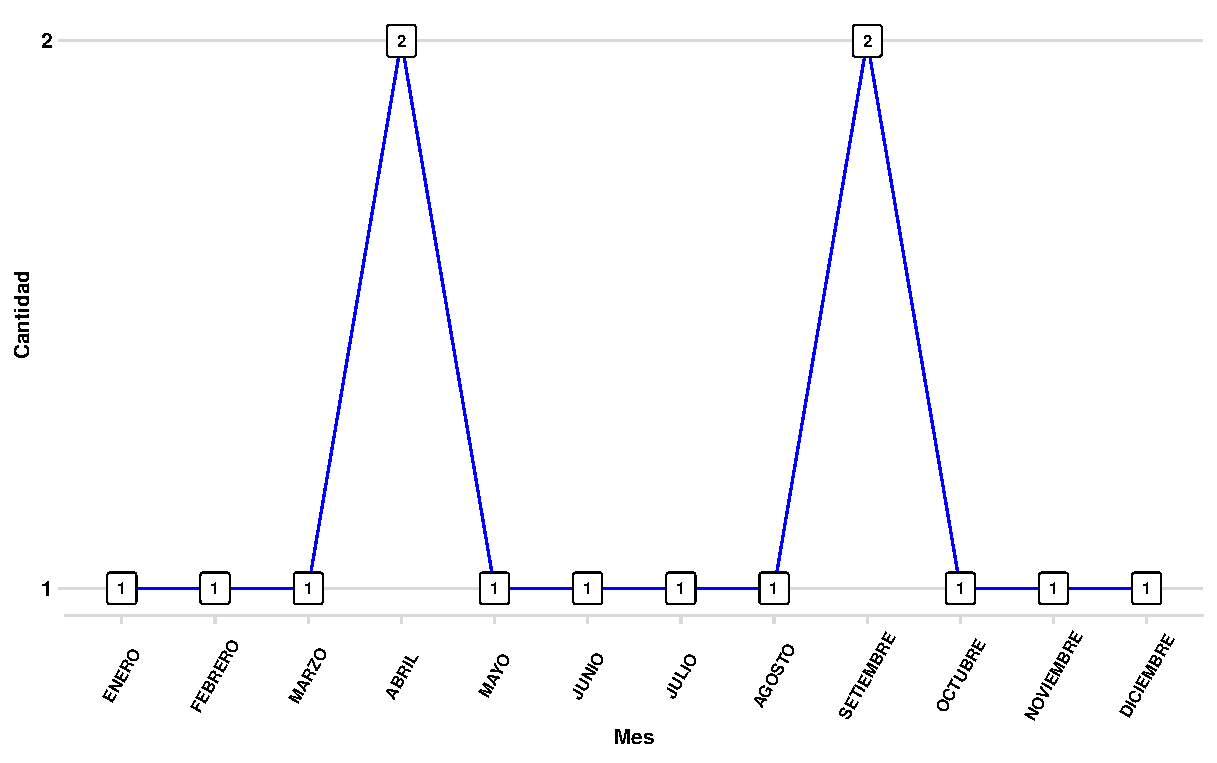
\includegraphics[width=15cm, height=5.95cm]{images/PROD014_demanda.pdf}}
  \label{fig:PROD014_demanda}
\end{figure}

La Figura \ref{fig:PROD014_demanda} muestra el diagrama de lineas que representa la evolución de la demanda del toner TNP80C cyan por mes en el año 2024, se observa que la demanda tiene un comportamiento determinístico y sin estacionariedad ya que parece constante en los meses sin tendencia, tomando estos casos y el comportamiento de la demanda es necesario utilizar un \textsl{modelo determinístico EOQ}.

Tomando en cuenta la demanda total anual de la Tabla \ref{table:GrupoA_Area}, el costo de compra de la Tabla \ref{table:GrupoA_Costo_Compra}, el costo de preparación estimado de la Tabla \ref{table:GrupoA_Costo_Preparacion}, el costo de retención estimado de la Tabla \ref{table:GrupoA_Costo_Retencion} y tiempo de reabastecimiento del pedido brindado por el área de logística se tienen los siguientes valores:

\begin{itemize}
    \item \textbf{Demanda ($D$):} 14 unidades
    \item \textbf{Costo de compra ($C$):} S/ 715.00 por unidad
    \item \textbf{Costo de preparación ($K$):} S/ 9.61
    \item \textbf{Costo de retención ($h$):} S/ 7.76
    \item \textbf{Tiempo de entrega ($L$):} 1 día
\end{itemize}

Hallamos la cantidad de pedido óptima $y^*$ mediante la expresión (\ref{yopt}) de la siguiente manera
\begin{eqnarray}
    y^* &=& \sqrt{\frac{2KD}{h}} \nonumber
\end{eqnarray}
\begin{eqnarray}
    y^* &=& \sqrt{\frac{2(9.61)(14)}{7.76}} \nonumber \\
    y^* &=& 5.89 \nonumber \\
    y^* &\thickapprox& 6 \text{ unidades} \nonumber
\end{eqnarray}
De la misma forma hallemos el intervalo de pedido óptimo $T^*$ utilizando la expresión (\ref{Topt}) 
\begin{eqnarray}
    T^* &=& \sqrt{\frac{2K}{Dh}} \nonumber \\
    T^* &=& \sqrt{\frac{2(9.61)}{(14)(7.76)}} \nonumber \\
    T^* &=& 0.4206 \nonumber
\end{eqnarray}
Asimismo tomemos la demanda por día laborable (52 semanas * 5 días/semana = 260 días laborables) de tal forma que vemos el momento de cuando pedir
\begin{eqnarray}
    T^* &=& 0.4206 (260 \text{ días laborables}) \nonumber \\   
    T^* &=& 109.36 \nonumber \\
    T^* &\thickapprox& 109 \text{ días laborables} \nonumber
\end{eqnarray}
Ahora hallemos el costo mínimo total de inventario óptimo $CTI(y^*)$ usando la expresión (\ref{CTIopt}).
\begin{eqnarray}
    CTI(y^*) &=& \sqrt{2hKD} + DC \nonumber \\
    CTI(y^*) &=& \sqrt{2(7.76)(9.61)(14)} + (14)(715) \nonumber \\
    CTI(y^*) &=& \text{S/ 10,055.70} \nonumber
\end{eqnarray}
Por último hallemos el punto de reorden en base a la cantidad de pedido óptima y el tiempo de reabastecimiento de 1 día.
\begin{eqnarray}
    R &=& L_e D \nonumber \\
    R &=& (1) \left(\frac{14}{260 \text{ días laborables}} \right) \nonumber
\end{eqnarray}
\begin{eqnarray}
    R &=& 0.05 \nonumber \\
    R &\thickapprox& 0 \text{ unidades} \nonumber
\end{eqnarray}

Esto quiere decir que cuando el inventario del producto llegue a 0 unidades se deben de realizar el pedido de 6 unidades, del cual el tiempo de pedido debería ser cada 109 días laborables teniendo un costo total de S/ 10,055.70
\subsubsection{Solución salina equilibrada (BSS) en botella de vidrio 500 ml}

El producto solución salina equilibrada (BSS) en botella de vidrio de 500 ml de Catarata del área de oftalmología es utilizado generalmente en las cirugías del área de oftalmología realizadas, primeramente observemos la tendencia de la demanda a lo largo del año 2024 en el siguiente gráfico.

\begin{figure}[H]
  \caption{Evolución demanda: Solución salina equilibrada (BSS) en botella de vidrio 500 ml de Catarata - oftalmología}
  {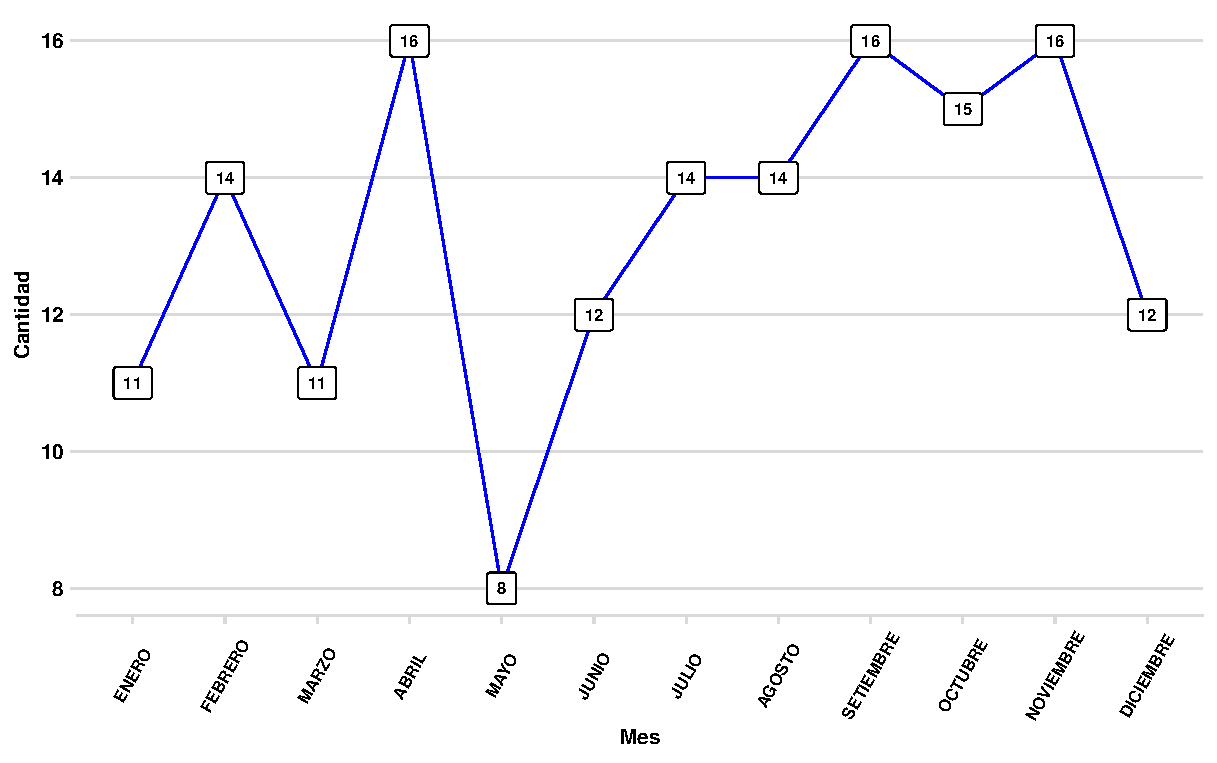
\includegraphics[width=15cm, height=5.95cm]{images/PROD015_demanda.pdf}}
  \label{fig:PROD015_demanda}
\end{figure}

La Figura \ref{fig:PROD015_demanda} muestra el diagrama de lineas que representa la evolución de la demanda sobre la solución salina equilibrada (BSS) por mes en el año 2024, se observa que la demanda tiene un comportamiento determinístico a través de los meses del año, a excepción del mes de mayo en donde se encuentra el valor más bajo, asimismo no se observa una tendencia y solo estacionariedad en el tiempo, por lo que tomando estos casos y el comportamiento de la demanda es necesario utilizar un \textsl{modelo determinístico EOQ}.

Tomando en cuenta la demanda total anual de la Tabla \ref{table:GrupoA_Area}, el costo de compra de la Tabla \ref{table:GrupoA_Costo_Compra}, el costo de preparación estimado de la Tabla \ref{table:GrupoA_Costo_Preparacion}, el costo de retención estimado de la Tabla \ref{table:GrupoA_Costo_Retencion} y tiempo de reabastecimiento del pedido brindado por el área de logística se tienen los siguientes valores:

\begin{itemize}
    \item \textbf{Demanda ($D$):} 159 unidades
    \item \textbf{Costo de compra ($C$):} S/ 290.00 por unidad
    \item \textbf{Costo de preparación ($K$):} S/ 5.80
    \item \textbf{Costo de retención ($h$):} S/ 18.19
    \item \textbf{Tiempo de entrega ($L$):} 7 días
\end{itemize}

Hallamos la cantidad de pedido óptima $y^*$ mediante la expresión (\ref{yopt}) de la siguiente manera
\begin{eqnarray}
    y^* &=& \sqrt{\frac{2KD}{h}} \nonumber \\
    y^* &=& \sqrt{\frac{2(5.8)(159)}{18.19}} \nonumber \\
    y^* &=& 10.07 \nonumber \\
    y^* &\thickapprox& 10 \text{ unidades} \nonumber
\end{eqnarray}
De la misma forma hallemos el intervalo de pedido óptimo $T^*$ utilizando la expresión (\ref{Topt}) 
\begin{eqnarray}
    T^* &=& \sqrt{\frac{2K}{Dh}} \nonumber \\
    T^* &=& \sqrt{\frac{2(5.8)}{(159)(18.19)}} \nonumber \\
    T^* &=& 0.0633 \nonumber
\end{eqnarray}
Asimismo tomemos la demanda por día laborable (52 semanas * 5 días/semana = 260 días laborables) de tal forma que vemos el momento de cuando pedir
\begin{eqnarray}
    T^* &=& 0.0633 (260 \text{ días laborables}) \nonumber
\end{eqnarray}
\begin{eqnarray}
    T^* &=& 16.47 \nonumber \\
    T^* &\thickapprox& 16 \text{ días laborables} \nonumber
\end{eqnarray}
Ahora hallemos el costo mínimo total de inventario óptimo $CTI(y^*)$ usando la expresión (\ref{CTIopt}).
\begin{eqnarray}
    CTI(y^*) &=& \sqrt{2hKD} + DC \nonumber \\
    CTI(y^*) &=& \sqrt{2(18.19)(5.8)(159)} + (159)(290) \nonumber \\
    CTI(y^*) &=& \text{S/ 46,293.17} \nonumber
\end{eqnarray}
Por último hallemos el punto de reorden en base a la cantidad de pedido óptima y el tiempo de reabastecimiento de 7 días.
\begin{eqnarray}
    R &=& L_e D \nonumber \\
    R &=& (7) \left(\frac{159}{260 \text{ días laborables}} \right) \nonumber \\
    R &=& 4.28 \nonumber \\
    R &\thickapprox& 4 \text{ unidades} \nonumber
\end{eqnarray}

Esto quiere decir que cuando el inventario del producto llegue a 4 unidades se deben de realizar el pedido de 10 unidades, del cual el tiempo de pedido debería ser cada 16 días laborables teniendo un costo total de S/ 46,293.17
\subsubsection{Campo quirúrgico 100 x 120 cm}

El producto campo quirúrgico 100 x 120 cm de Insumos generales del área de oftalmología es utilizado generalmente en las cirugías del área de oftalmología realizadas, primeramente observemos la tendencia de la demanda a lo largo del año 2024 en el siguiente gráfico.
\clearpage
\begin{figure}[H]
  \caption{Evolución demanda: Campo quirúrgico 100 x 120 cm de Insumos generales - oftalmología}
  {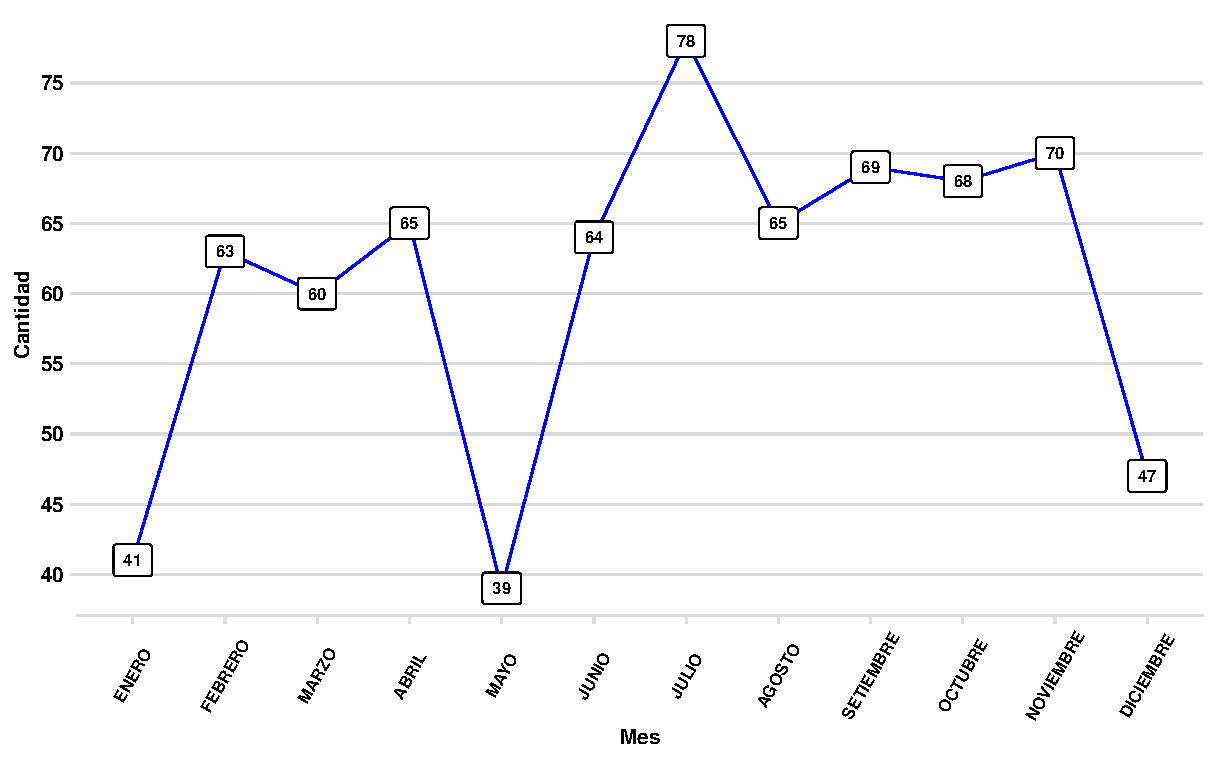
\includegraphics[width=15cm, height=5.95cm]{images/PROD016_demanda.pdf}}
  \label{fig:PROD016_demanda}
\end{figure}

La Figura \ref{fig:PROD016_demanda} muestra el diagrama de lineas que representa la evolución de la demanda del campo quirúrgico 100 x 120 cm por mes en el año 2024, se observa que la demanda tiene un comportamiento determinístico a través de los meses del año, a excepción de los meses de enero, mayo y diciembre en los cuales se presentan valores extremos bajos, asimismo no se observa una tendencia y solo estacionariedad en el tiempo, por lo que tomando estos casos y el comportamiento de la demanda es necesario utilizar un \textsl{modelo determinístico EOQ}.

Tomando en cuenta la demanda total anual de la Tabla \ref{table:GrupoA_Area}, el costo de compra de la Tabla \ref{table:GrupoA_Costo_Compra}, el costo de preparación estimado de la Tabla \ref{table:GrupoA_Costo_Preparacion}, el costo de retención estimado de la Tabla \ref{table:GrupoA_Costo_Retencion} y tiempo de reabastecimiento del pedido brindado por el área de logística se tienen los siguientes valores:

\begin{itemize}
    \item \textbf{Demanda ($D$):} 729 unidades
    \item \textbf{Costo de compra ($C$):} S/ 14.00 por unidad
    \item \textbf{Costo de preparación ($K$):} S/ 3.80
    \item \textbf{Costo de retención ($h$):} S/ 2.14
    \item \textbf{Tiempo de entrega ($L$):} 7 días
\end{itemize}

Hallamos la cantidad de pedido óptima $y^*$ mediante la expresión (\ref{yopt}) de la siguiente manera
\clearpage
\begin{eqnarray}
    y^* &=& \sqrt{\frac{2KD}{h}} \nonumber \\
    y^* &=& \sqrt{\frac{2(3.8)(729)}{2.14}} \nonumber \\
    y^* &=& 50.88 \nonumber \\
    y^* &\thickapprox& 51 \text{ unidades} \nonumber
\end{eqnarray}
De la misma forma hallemos el intervalo de pedido óptimo $T^*$ utilizando la expresión (\ref{Topt}) 
\begin{eqnarray}
    T^* &=& \sqrt{\frac{2K}{Dh}} \nonumber \\
    T^* &=& \sqrt{\frac{2(3.8)}{(729)(2.14)}} \nonumber \\
    T^* &=& 0.0698 \nonumber
\end{eqnarray}
Asimismo tomemos la demanda por día laborable (52 semanas * 5 días/semana = 260 días laborables) de tal forma que vemos el momento de cuando pedir
\begin{eqnarray}
    T^* &=& 0.0698 (260 \text{ días laborables}) \nonumber \\   
    T^* &=& 18.15 \nonumber \\
    T^* &\thickapprox& 18 \text{ días laborables} \nonumber
\end{eqnarray}
Ahora hallemos el costo mínimo total de inventario óptimo $CTI(y^*)$ usando la expresión (\ref{CTIopt}).
\begin{eqnarray}
    CTI(y^*) &=& \sqrt{2hKD} + DC \nonumber \\
    CTI(y^*) &=& \sqrt{2(2.14)(3.8)(729)} + (729)(14) \nonumber \\
    CTI(y^*) &=& \text{S/ 10,314.89} \nonumber
\end{eqnarray}
Por último hallemos el punto de reorden en base a la cantidad de pedido óptima y el tiempo de reabastecimiento de 7 días.
\clearpage
\begin{eqnarray}
    R &=& L_e D \nonumber \\
    R &=& (7) \left(\frac{729}{260 \text{ días laborables}} \right) \nonumber \\
    R &=& 19.63 \nonumber \\
    R &\thickapprox& 20 \text{ unidades} \nonumber
\end{eqnarray}

Esto quiere decir que cuando el inventario del producto llegue a 20 unidades se deben de realizar el pedido de 51 unidades, del cual el tiempo de pedido debería ser cada 18 días laborables teniendo un costo total de S/ 10,314.89
\subsubsection{Azul de tripan 0.06$\%$ - 0.6 mg VIAL x 1ml / OCUBLU - TRY}

El producto azul de tripan 0.06$\%$ - 0.6 mg VIAL x 1 ml de Catarata del área de oftalmología es utilizado para la cirugía de facoemulsificación y extracción manual de catarata con incisión pequeña que son las cirugías para la extracción de la catarata, primeramente observemos la tendencia de la demanda a lo largo del año 2024 en el siguiente gráfico.

\begin{figure}[H]
  \caption{Evolución demanda: Azul de tripan 0.06$\%$ - 0.6 mg VIAL x 1 ml / OCUBLU - TRY de Catarata - oftalmología}
  {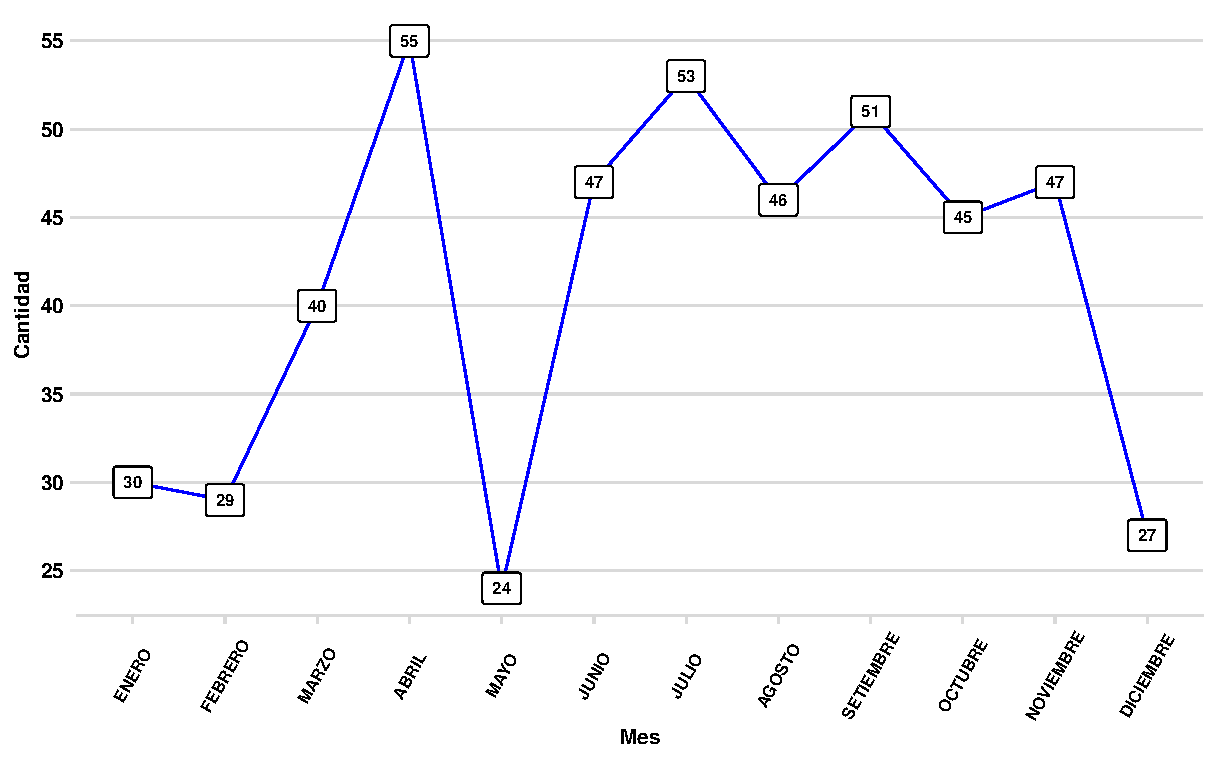
\includegraphics[width=15cm, height=5.95cm]{images/PROD017_demanda.pdf}}
  \label{fig:PROD017_demanda}
\end{figure}

La Figura \ref{fig:PROD017_demanda} muestra el diagrama de lineas que representa la evolución de la demanda del azul de tripan 0.06$\%$ por mes en el año 2024, se observa que la demanda tiene un comportamiento determinístico a través de los meses del año, a excepción de los meses de enero, febrero, mayo y diciembre en los cuales se tienen valores extremos bajos, asimismo no se observa una tendencia y solo estacionariedad en el tiempo, por lo que tomando estos casos y el comportamiento de la demanda es necesario utilizar un \textsl{modelo determinístico EOQ}.

Tomando en cuenta la demanda total anual de la Tabla \ref{table:GrupoA_Area}, el costo de compra de la Tabla \ref{table:GrupoA_Costo_Compra}, el costo de preparación estimado de la Tabla \ref{table:GrupoA_Costo_Preparacion}, el costo de retención estimado de la Tabla \ref{table:GrupoA_Costo_Retencion} y tiempo de reabastecimiento del pedido brindado por el área de logística se tienen los siguientes valores:

\begin{itemize}
    \item \textbf{Demanda ($D$):} 494 unidades
    \item \textbf{Costo de compra ($C$):} S/ 400.00 por unidad
    \item \textbf{Costo de preparación ($K$):} S/ 9.61
    \item \textbf{Costo de retención ($h$):} S/ 2.41
    \item \textbf{Tiempo de entrega ($L$):} 7 días
\end{itemize}

Hallamos la cantidad de pedido óptima $y^*$ mediante la expresión (\ref{yopt}) de la siguiente manera
\begin{eqnarray}
    y^* &=& \sqrt{\frac{2KD}{h}} \nonumber \\
    y^* &=& \sqrt{\frac{2(9.61)(494)}{2.41}} \nonumber \\
    y^* &=& 62.77 \nonumber \\
    y^* &\thickapprox& 63 \text{ unidades} \nonumber
\end{eqnarray}
De la misma forma hallemos el intervalo de pedido óptimo $T^*$ utilizando la expresión (\ref{Topt}) 
\begin{eqnarray}
    T^* &=& \sqrt{\frac{2K}{Dh}} \nonumber \\
    T^* &=& \sqrt{\frac{2(9.61)}{(494)(2.41)}} \nonumber \\
    T^* &=& 0.1271 \nonumber
\end{eqnarray}
\clearpage
\noindent Asimismo tomemos la demanda por día laborable (52 semanas * 5 días/semana = 260 días laborables) de tal forma que vemos el momento de cuando pedir
\begin{eqnarray}
    T^* &=& 0.1271 (260 \text{ días laborables}) \nonumber \\   
    T^* &=& 33.04 \nonumber \\
    T^* &\thickapprox& 33 \text{ días laborables} \nonumber
\end{eqnarray}
Ahora hallemos el costo mínimo total de inventario óptimo $CTI(y^*)$ usando la expresión (\ref{CTIopt}).
\begin{eqnarray}
    CTI(y^*) &=& \sqrt{2hKD} + DC \nonumber \\
    CTI(y^*) &=& \sqrt{2(2.41)(9.61)(494)} + (494)(400) \nonumber \\
    CTI(y^*) &=& \text{S/ 197,751.27} \nonumber
\end{eqnarray}
Por último hallemos el punto de reorden en base a la cantidad de pedido óptima y el tiempo de reabastecimiento de 7 días.
\begin{eqnarray}
    R &=& L_e D \nonumber \\
    R &=& (7) \left(\frac{494}{260 \text{ días laborables}} \right) \nonumber \\
    R &=& 13.30 \nonumber \\
    R &\thickapprox& 13 \text{ unidades} \nonumber
\end{eqnarray}

Esto quiere decir que cuando el inventario del producto llegue a 13 unidades se deben de realizar el pedido de 63 unidades, del cual el tiempo de pedido debería ser cada 33 días laborables teniendo un costo total de S/ 197,751.27

\subsubsection{Agua destilada y/o desionizada}

El producto agua destilada y/o desionizada de Esterilización del área de oftalmología es utilizado para el área de oftalmología en los procedimientos realizados, primeramente observemos la tendencia de la demanda a lo largo del año 2024 en el siguiente gráfico.
\clearpage
\begin{figure}[H]
  \caption{Evolución demanda: Agua destilada y/o desionizada de Esterilización - oftalmología}
  {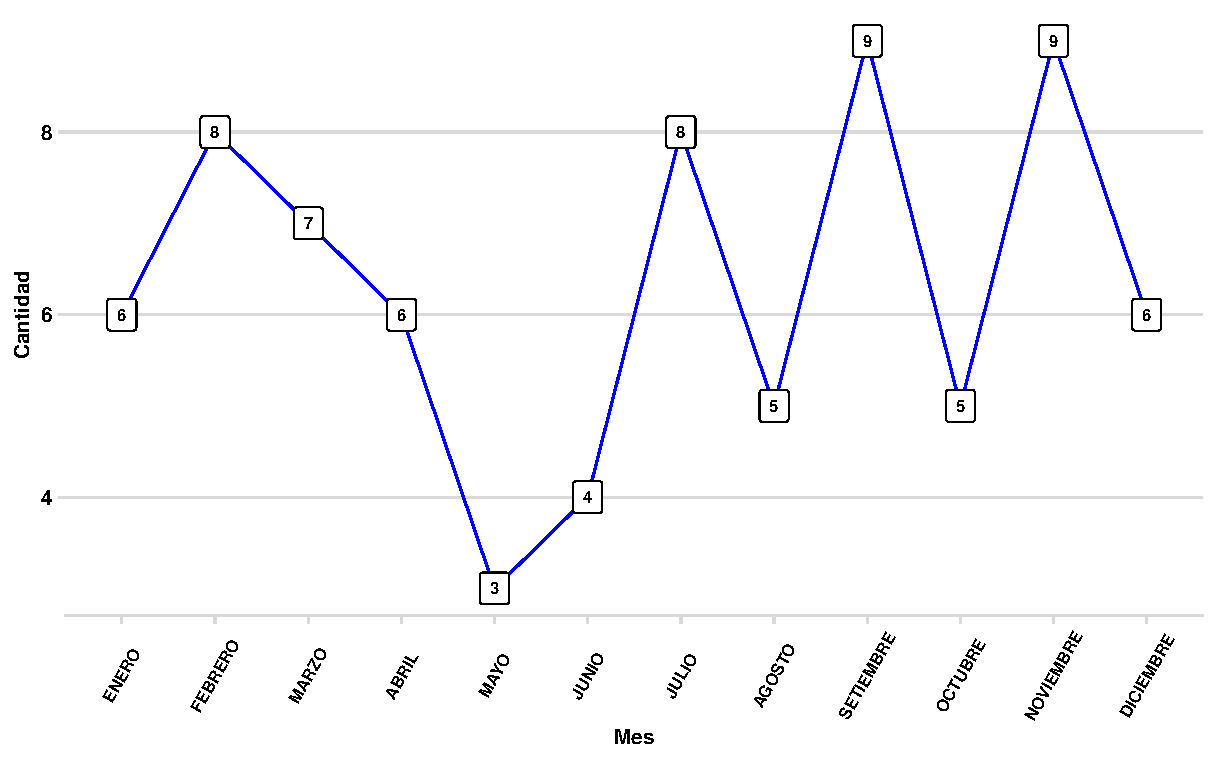
\includegraphics[width=15cm, height=5.95cm]{images/PROD018_demanda.pdf}}
  \label{fig:PROD018_demanda}
\end{figure}

La Figura \ref{fig:PROD018_demanda} muestra el diagrama de lineas que representa la evolución de la demanda del agua destilada por mes en el año 2024, se observa que la demanda tiene un comportamiento determinístico a través de los meses del año, a excepción del mes de mayo en donde se tuvo el punto más bajo, asimismo no se observa una tendencia y solo estacionariedad en el tiempo, por lo que tomando estos casos y el comportamiento de la demanda es necesario utilizar un \textsl{modelo determinístico EOQ}.

Tomando en cuenta la demanda total anual de la Tabla \ref{table:GrupoA_Area}, el costo de compra de la Tabla \ref{table:GrupoA_Costo_Compra}, el costo de preparación estimado de la Tabla \ref{table:GrupoA_Costo_Preparacion}, el costo de retención estimado de la Tabla \ref{table:GrupoA_Costo_Retencion} y tiempo de reabastecimiento del pedido brindado por el área de logística se tienen los siguientes valores:

\begin{itemize}
    \item \textbf{Demanda ($D$):} 76 unidades
    \item \textbf{Costo de compra ($C$):} S/ 39.84 por unidad
    \item \textbf{Costo de preparación ($K$):} S/ 11.51
    \item \textbf{Costo de retención ($h$):} S/ 473.40
    \item \textbf{Tiempo de entrega ($L$):} 7 días
\end{itemize}

Hallamos la cantidad de pedido óptima $y^*$ mediante la expresión (\ref{yopt}) de la siguiente manera
\clearpage
\begin{eqnarray}
    y^* &=& \sqrt{\frac{2KD}{h}} \nonumber \\
    y^* &=& \sqrt{\frac{2(11.51)(76)}{473.4}} \nonumber \\
    y^* &=& 1.92 \nonumber \\
    y^* &\thickapprox& 2 \text{ unidades} \nonumber
\end{eqnarray}
De la misma forma hallemos el intervalo de pedido óptimo $T^*$ utilizando la expresión (\ref{Topt}) 
\begin{eqnarray}
    T^* &=& \sqrt{\frac{2K}{Dh}} \nonumber \\
    T^* &=& \sqrt{\frac{2(11.51)}{(76)(473.4)}} \nonumber \\
    T^* &=& 0.0253 \nonumber
\end{eqnarray}
Asimismo tomemos la demanda por día laborable (52 semanas * 5 días/semana = 260 días laborables) de tal forma que vemos el momento de cuando pedir
\begin{eqnarray}
    T^* &=& 0.0253 (260 \text{ días laborables}) \nonumber \\   
    T^* &=& 6.58 \nonumber \\
    T^* &\thickapprox& 7 \text{ días laborables} \nonumber
\end{eqnarray}
Ahora hallemos el costo mínimo total de inventario óptimo $CTI(y^*)$ usando la expresión (\ref{CTIopt}).
\begin{eqnarray}
    CTI(y^*) &=& \sqrt{2hKD} + DC \nonumber \\
    CTI(y^*) &=& \sqrt{2(473.4)(11.51)(76)} + (76)(39.84) \nonumber \\
    CTI(y^*) &=& \text{S/ 3,937.91} \nonumber
\end{eqnarray}
Por último hallemos el punto de reorden en base a la cantidad de pedido óptima y el tiempo de reabastecimiento de 7 días.
\clearpage
\begin{eqnarray}
    R &=& L_e D \nonumber \\
    R &=& (7) \left(\frac{76}{260 \text{ días laborables}} \right) \nonumber \\
    R &=& 2.05 \nonumber \\
    R &\thickapprox& 2 \text{ unidades} \nonumber
\end{eqnarray}

Esto quiere decir que cuando el inventario del producto llegue a 2 unidades se deben de realizar el pedido de 2 unidades, del cual el tiempo de pedido debería ser cada 7 días laborables teniendo un costo total de S/ 3,937.91

\section{Generación del aplicativo web}
Como última parte se generará el aplicativo en Shiny que ayudará en el seguimiento no solo de los productos analizados anteriormente, sino también de nuevos productos que el centro de salud también requiera aplicar en su política de inventarios.

El aplicativo se desarrolló en el lenguaje R debido a su potencia en análisis estadístico y modelado matemático, permitiendo combinar de manera eficiente cálculos, visualizaciones y lógica de decisión en un solo entorno. De tal forma que se contribuye a la optimización de procesos de gestión de inventarios al facilitar una interfaz intuitiva para el usuario que automatize tareas que requieran intervención manual.

Para el desarrollo se empleó \textsl{RShiny}, un paquete de R que permite la creación de aplicaciones web interactivas, el cual tuvo las siguientes etapas:

\begin{enumerate}
    \item Diseño de la interfaz de usuario \textsl{(UI)} en el que se definieron los menús, paneles, filtros, ubicación de gráficos y tablas.
    \item Definición del servidor \textsl{(server)} en el que colocaron las funciones para procesar la lógica computacional, conectando los inputs del usuario con los outputs correspondientes.
    \item Carga y limpieza de datos en el que se tiene el procesamiento del archivo que se subirá para realizar el análisis, así como las debidas transformaciones y funciones que sean necesarias.
    \item Implementación de modelo de inventarios en el que se crearon funciones para realizar las políticas de inventarios tomando en cuenta el modelo EOQ clásico, EOQ con escasez y EOQ probabilizado.
    \item Visualización de resultados a través de gráficos, tablas e informaciones que permitan el monitoreo del inventario.
    \item Pruebas funcionales realizadas para asegurar la estabilidad de la aplicación y validación que pueda necesitar.
    \item Despliegue del aplicativo, ejecutandose en el servidor de Shiny con el plan básico gratuito, el enlace del aplicativo es el siguiente \url{https://kevin-heberth-haquehua-apaza.shinyapps.io/App_Inventario_Fuente_UNSAAC/}
\end{enumerate}

\subsection{Presentación del aplicativo}
Como primera parte se tiene la presentación del aplicativo web, mostrado cuando se accede al enlace, en esta parte se da una breve reseña de las funciones que contiene el aplicativo de inventario.
\begin{figure}[H]
  \caption{Información general del aplicativo de inventario}
  {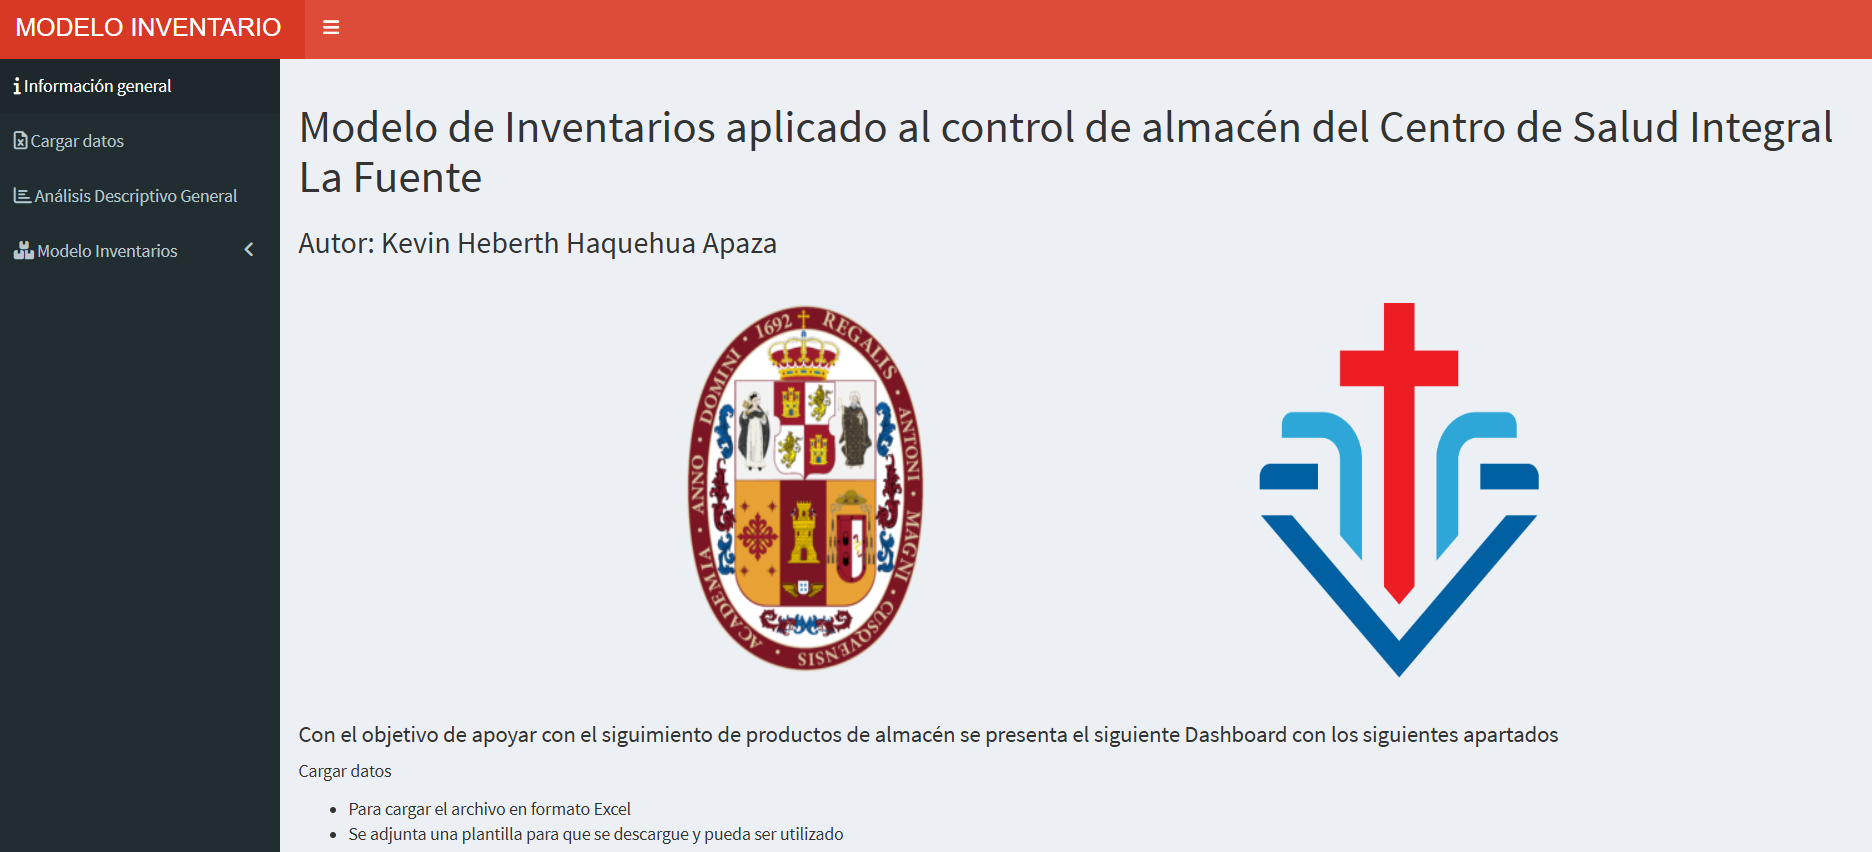
\includegraphics[width=15cm, height=6.85cm]{images/Shiny1.png}}
  \label{fig:Shiny1}
\end{figure}

La Figura \ref{fig:Shiny1} muestra la presentación del aplicativo cuando se accede al enlace proporcionado, asimismo muestra un breve resumen de las funciones que tiene el aplicativo.

\subsection{Cargar datos}
Accediendo a la segunda pestaña del aplicativo ``Cargar datos'', se muestra la parte en donde se tiene que subir los datos para que pueda ser ejecutado el análisis

\begin{figure}[H]
  \caption{Cargar datos del aplicativo de inventario}
  {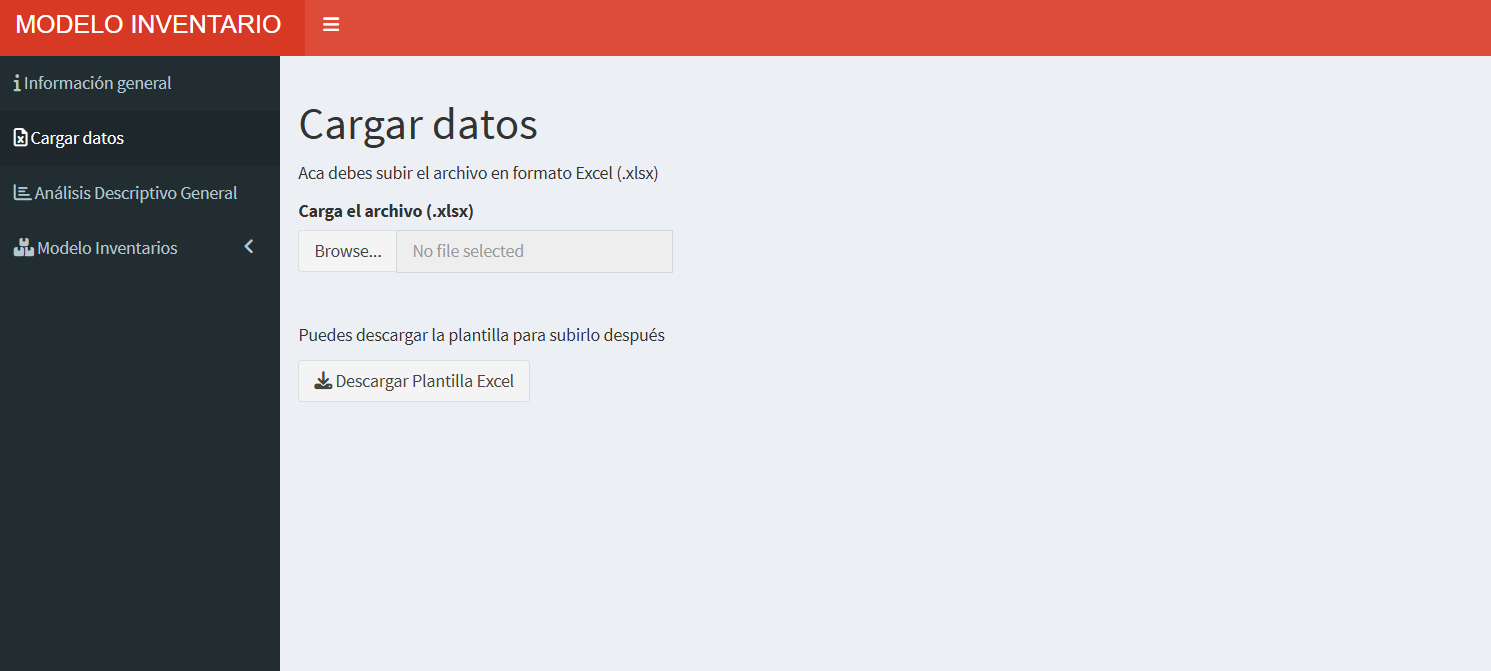
\includegraphics[width=16cm, height=9cm]{images/Shiny2.png}}
  \label{fig:Shiny2}
\end{figure}

La Figura \ref{fig:Shiny2} muestra la sección de cargar datos que viene a ser la primera parte que se debe de realizar, los puntos a tener en cuenta son los siguientes:

\begin{itemize}
  \item La extensión en la que debe subirse el archivo de carga es la extensión \textsl{.xlsx} que viene a ser el formato de archivos Excel.
  \item Asimismo el archivo debe tener dos hojas, en la cual la primera parte debe tener la información de todos los productos: Identificador del producto \textsl{(IDPROD)}, área al que pertenece el producto \textsl{(AREA)}, especialidad al que pertenece el producto \textsl{(ESPECIALIDAD)}, denominación del producto \textsl{(PRODUCTO)}, volumen que ocupa el producto en $cm^3$ \textsl{(VOLUMEN)}, cantidad de pedidos realizados por el producto, aunque este apartado no es tan necesario \textsl{(PEDIDOS)}, costo total del producto en el periodo de tiempo \textsl{(COSTO)}.
  \item La segunda hoja debe tener la demanda de los costos en la cual se debe tener la siguiente información: Identificador del producto el cual debe ser el mismo que el colocado en la primera hoja \textsl{(IDPROD)}, demanda evaluada por el periodo de tiempo (en este caso por meses), volumen que ocupa el producto en $cm^3$ \textsl{(VOLUMEN)}, el costo de compra del producto \textsl{(COSTO\_COMPRA\_C)}, el costo de preparación del producto \textsl{(COSTO\_PREPARACION\_K)}, el costo de retención del producto \textsl{(COSTO\_RETENCION\_h)}, el costo de escasez del producto \textsl{(COSTO\_ESCASEZ\_p)}, tiempo de entrega del pedido \textsl{(TIEMPO\_ENTREGA\_L)}
  \item Una mejor forma de ver el tipo de archivo que se debe subir se puede encontrar en el ANEXO G en donde se muestra la base de datos para realizar el estudio.
  \item De la misma forma en la parte inferior se puede descargar una plantilla con la información solicitada para que se pueda ingresar información y posteriormente subirlo.
  \item Es muy importante que el archivo Excel que se suba al aplicativo contenga la información solicitada que se detalló anteriormente, caso contrario no podrá realizar el análisis y modelos de inventarios.
\end{itemize}

\subsection{Análisis descriptivo general}
Una vez subido el archivo solicitado se tiene que ir a la parte de análisis descriptivo general en donde en base a la primera hoja llenada, mostrará un resumen descriptivo de las áreas y especialidades en base a los costos, y por último mostrará el análisis basado en costos (ABC) de los productos y su categorización.

\subsubsection{Análisis descriptivo por área}
En esta parte se muestra el análisis descriptivo por área tomando principalmente en cuenta los costos.

\begin{figure}[H]
  \caption{Análisis descriptivo general por área del aplicativo de inventario}
  {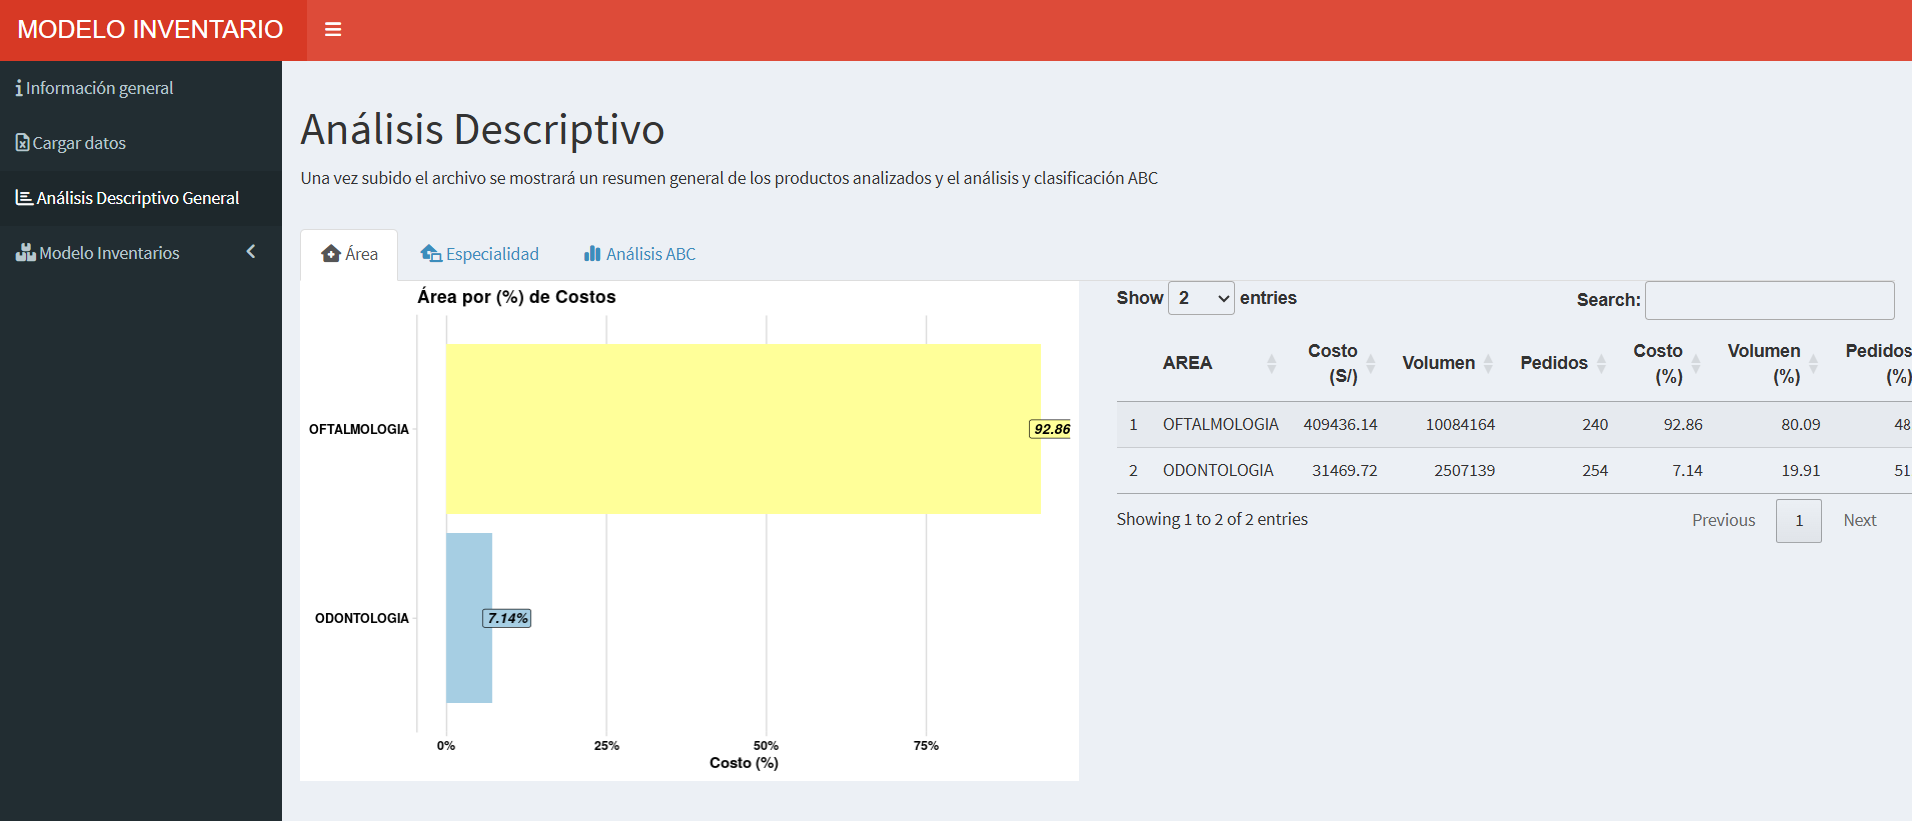
\includegraphics[width=16cm, height=10cm]{images/Shiny3.png}}
  \label{fig:Shiny3}
\end{figure}

La Figura \ref{fig:Shiny3} muestra el análisis por área tomando en cuenta todos los productos, el cual muestra la siguiente información:

\begin{itemize}
  \item En la izquierda se muestra el gráfico de barras que representa las áreas en donde se encuentra la mayor parte de los costos del inventario.
  \item En la derecha se muestra una tabla que resume las áreas tomando en cuenta los costos acumulados, volumen acumulado, pedidos realizados, costos acumulados ($\%$), volumen acumulado ($\%$) y pedidos realizados ($\%$)
\end{itemize}

\subsubsection{Análisis descriptivo por especialidad}
En esta parte se muestra el análisis descriptivo por especialidad tomando principalmente en cuenta los costos.
\clearpage
\begin{figure}[H]
  \caption{Análisis descriptivo general por especialidad del aplicativo de inventario}
  {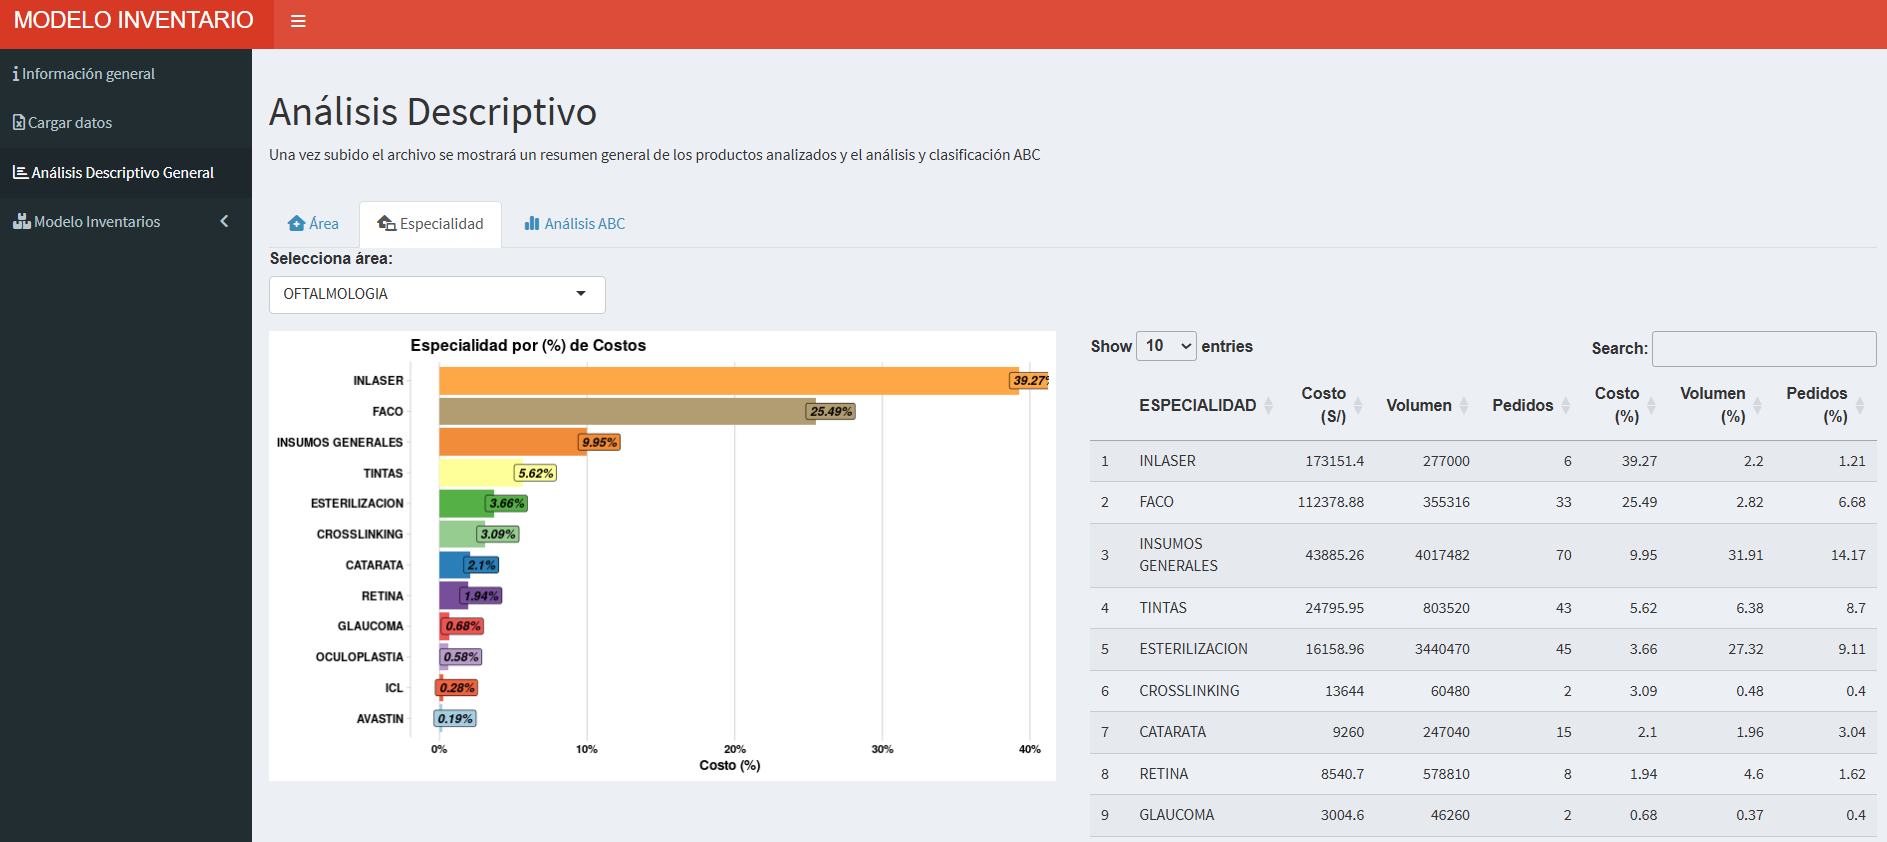
\includegraphics[width=16cm, height=10cm]{images/Shiny4.png}}
  \label{fig:Shiny4}
\end{figure}

La Figura \ref{fig:Shiny4} muestra el análisis por especialidad tomando en cuenta todos los productos, el cual muestra la siguiente información:

\begin{itemize}
  \item Primeramente se tiene un filtro para seleccionar un área y poder ver el análisis.
  \item En la izquierda se muestra el gráfico de barras que representa las especialidades en donde se encuentra la mayor parte de los costos del inventario.
  \item En la parte derecha se muestra una tabla que resume las especialidades tomando en cuenta los costos acumulados, volumen acumulado, pedidos realizados, costos acumulados ($\%$), volumen acumulado ($\%$) y pedidos realizados ($\%$)
\end{itemize}

\subsubsection{Análisis descriptivo por actividades basadas en costos (ABC)}
En esta parte se muestra el análisis de actividades basadas en costos (ABC) el cual el aplicativo es capaz de generar la clasificación de productos mediante la información brindada en los costos.
\clearpage
\begin{figure}[H]
  \caption{Análisis descriptivo de actividades basadas en costos (ABC) del aplicativo de inventario}
  {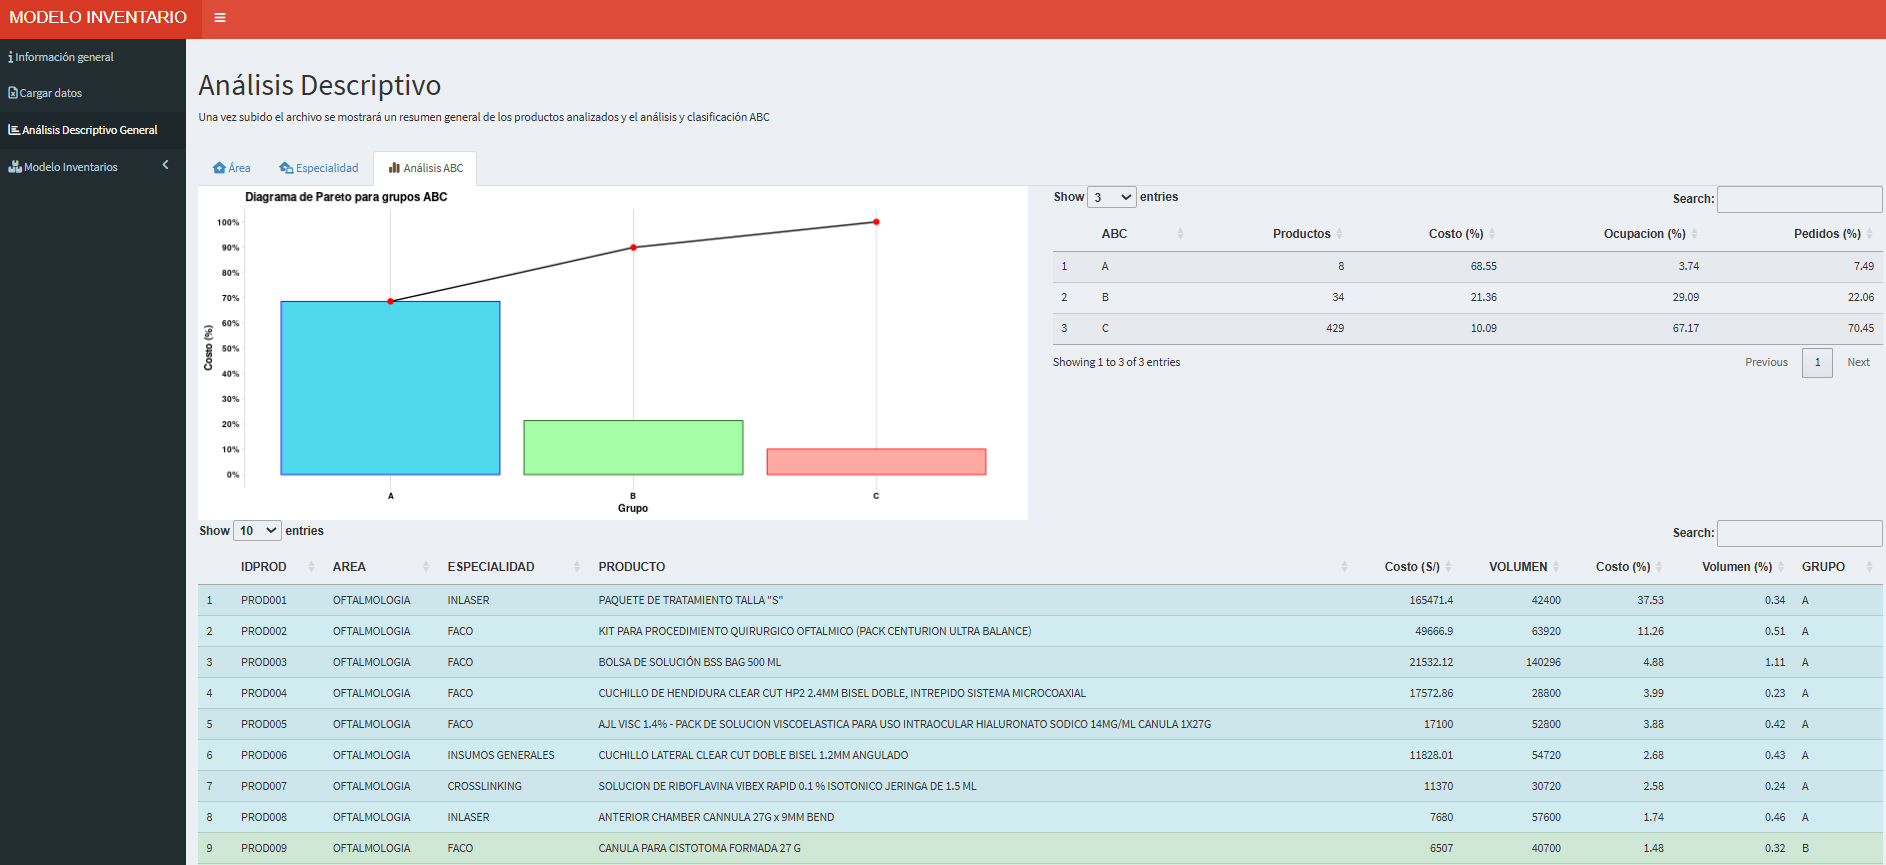
\includegraphics[width=16cm, height=10cm]{images/Shiny5.png}}
  \label{fig:Shiny5}
\end{figure}

La Figura \ref{fig:Shiny5} muestra el análisis de actividades basadas en costos (ABC) tomando en cuenta todos los productos, el cual muestra la siguiente información:

\begin{itemize}
  \item En la izquierda se muestra el diagrama de Pareto que representa los costos por grupos (A, B y C) en porcentaje de los costos.
  \item En la parte derecha se muestra una tabla que resume los resultados obtenidos mediante la clasificación (ABC) tomando en cuenta la cantidad de productos que tiene cada grupo, los costos acumulados ($\%$) en cada grupo, la ocupación que tiene cada grupo ($\%$) y los pedidos realizados por cada grupo ($\%$).
  \item En la parte inferior se muestra la lista de todos los productos, y de la misma forma a que grupo pertenece según la clasificación (ABC)
\end{itemize}
\clearpage
\subsection{Modelo de inventarios determinísticos}

La siguiente parte del análisis que brinda el aplicativo muestra la aplicación de la política de inventarios, primeramente tomando en cuenta los dos modelos determinísticos: EOQ clásico y EOQ con escasez.

\begin{figure}[H]
  \caption{Modelo determinístico del aplicativo de inventario}
  {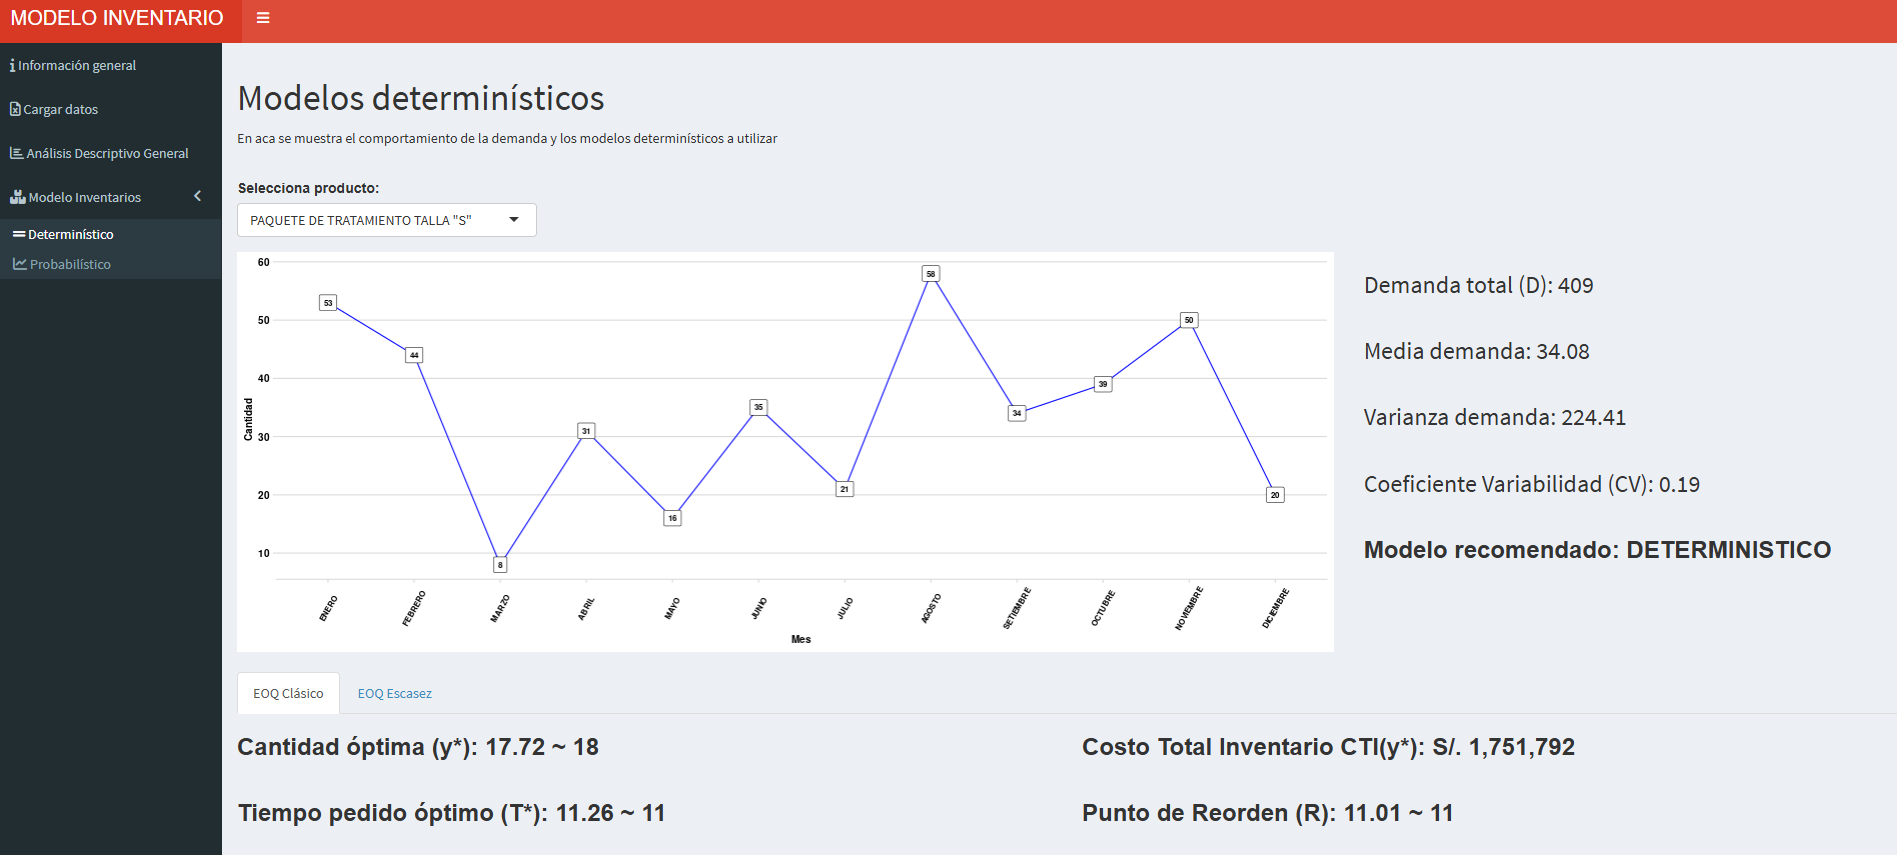
\includegraphics[width=16cm, height=10cm]{images/Shiny6.png}}
  \label{fig:Shiny6}
\end{figure}

La Figura \ref{fig:Shiny6} muestra los resultados de la aplicación del modelo de inventarios determinísticos en la cual se tiene la siguiente información:

\begin{itemize}
  \item En la parte principal se tiene un filtro que selecciona el producto al que se le va a aplicar el análisis y política de inventario óptima.
  \item En la izquierda se muestra un gráfico de línea que representa la demanda del producto por mes.
  \item En la derecha se muestra la información del producto en las cuales se tiene:
  \begin{itemize}
    \item \textbf{Demanda Total (D):} El cual representa la demanda total del periodo analizado, en este caso la demanda anual total.
    \item \textbf{Media demanda:} Representa la media de la demanda tomando en cuenta los periodos, en este caso la media de la demanda mensual.
    \item \textbf{Varianza demanda:} Representa la varianza de la demanda en el periodo analizado, en este caso la varianza de la demanda mensual.
    \item \textbf{Coeficiente de variabilidad (CV):} Representa el coeficiente de variabilidad calculado para ver si el modelo a usar es un determinístico ($CV < 0.20$) o un probabilístico ($CV \geq 0.20$).
    \item \textbf{Modelo recomendado:} Indica el modelo recomendado a utilizar (determinístico o probabilístico) tomando en cuenta el coeficiente de variabilidad.
  \end{itemize}
\end{itemize}


\subsubsection{Modelo clásico de cantidad económica de pedido (EOQ)}
La primera parte muestra los resultados aplicando el modelo determinístico EOQ clásico tomando en cuenta la información brindada en la sección (\ref{Modelo_clas_EOQ}) el cual muestra la siguiente información

\begin{itemize}
  \item \textbf{Cantidad óptima ($y^*$):} Muestra la cantidad óptima de pedido calculado mediante el modelo.
  \item \textbf{Tiempo pedido óptimo ($T^*$):} Muestra el tiempo de pedido óptimo para realizar el pedido del modelo.
  \item \textbf{Costo total inventario ($CTI(y^*)$):} Muestra el costo total que se obtendrá con la aplicación del modelo.
  \item \textbf{Punto de reorden (R):} Muestra el punto en la que debe de realizarse el siguiente pedido.
\end{itemize}

\subsubsection{Modelo clásico de cantidad económica de pedido (EOQ) con escasez}

La segunda parte muestra los resultados aplicando el modelo determinístico EOQ clásico con escasez, a pesar de que en los resultados obtenidos de los productos analizados no se tuvieron costos de escasez, es necesario colocar este análisis ya que el centro de salud puede agregar otros productos que necesite analizar su política de inventarios y tenga estos costos, para los resultados de este análisis se toma en cuenta la información de la sección (\ref{EOQ_escasez}) y seleccionando en el aplicativo la pestaña de EOQ Escasez.

\begin{figure}[H]
  \caption{Modelo determinístico EOQ con escasez del aplicativo de inventario}
  {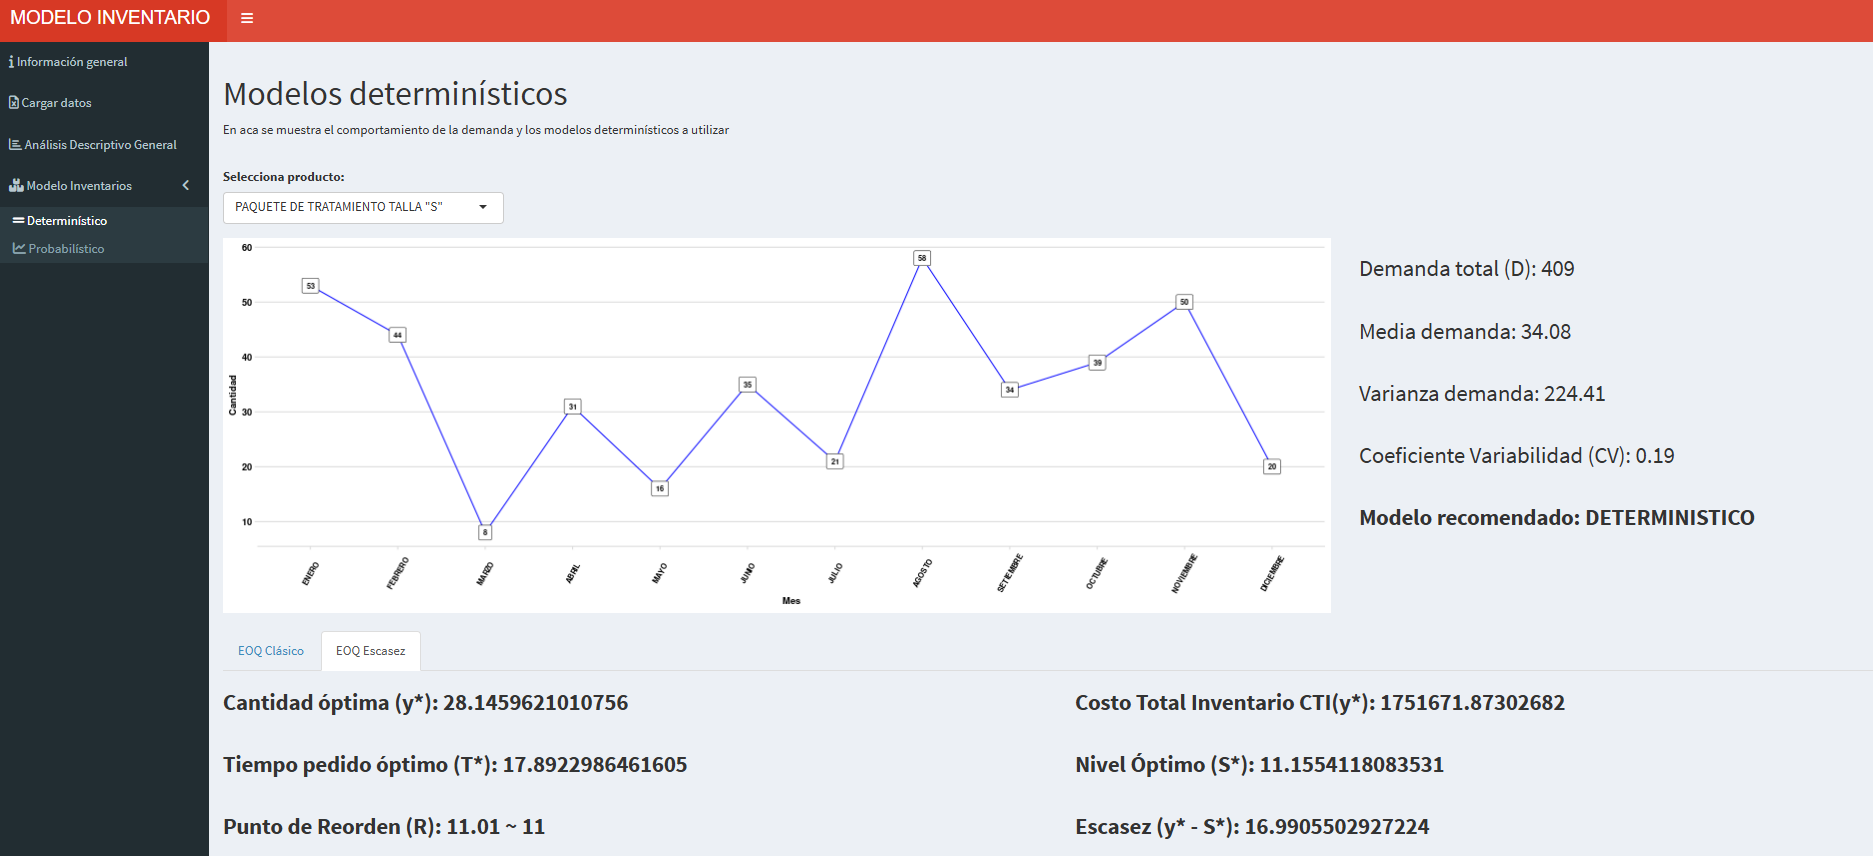
\includegraphics[width=16cm, height=10cm]{images/Shiny7.png}}
  \label{fig:Shiny7}
\end{figure}

La Figura \ref{fig:Shiny7} muestra los resultados tomando en cuenta el modelo EOQ con escasez, para mostrar el ejemplo se agrego al primer producto analizado un costo de escasez de S/ 6.50 en el cual la primera parte muestra la información general del modelo determinístico, la segunda parte muestra lo siguiente:

\begin{itemize}
   \item \textbf{Cantidad óptima ($y^*$):} Muestra la cantidad óptima de pedido calculado mediante el modelo.
  \item \textbf{Tiempo pedido óptimo ($T^*$):} Muestra el tiempo de pedido óptimo para realizar el pedido del modelo.
  \item \textbf{Costo total inventario ($CTI(y^*)$):} Muestra el costo total que se obtendrá con la aplicación del modelo.
  \item \textbf{Punto de reorden (R):} Muestra el punto en la que debe de realizarse el siguiente pedido.
  \item \textbf{Nivel Óptimo ($S^*$):} Muestra el nivel óptimo de inventario que se debe tener tomando en cuenta el modelo.
  \item \textbf{Nivel de escasez óptimo ($y^* - S^*$):} Muestra el nivel de escasez óptimo permitido aplicando el modelo.
\end{itemize}

\subsection{Modelo probabilístico}
La última parte que brinda el aplicativo es el análisis aplicando el modelo probabilístico usando la información brindada en la sección (\ref{EOQ_probabilizado}) el cual usa el modelo EOQ clásico tomando un nivel de reserva basándose en que la demanda se puede expresar mediante una distribución normal estándar, a pesar de que el coeficiente de variabilidad calculado indica que solo es necesario usar los modelos determinísticos, el centro de salud necesitaría también tomar en cuenta este modelo, especialmente para nuevos productos en los cuales se tenga un comportamiento probabilístico.

\begin{figure}[H]
  \caption{Modelo determinístico EOQ probabilizado del aplicativo de inventario}
  {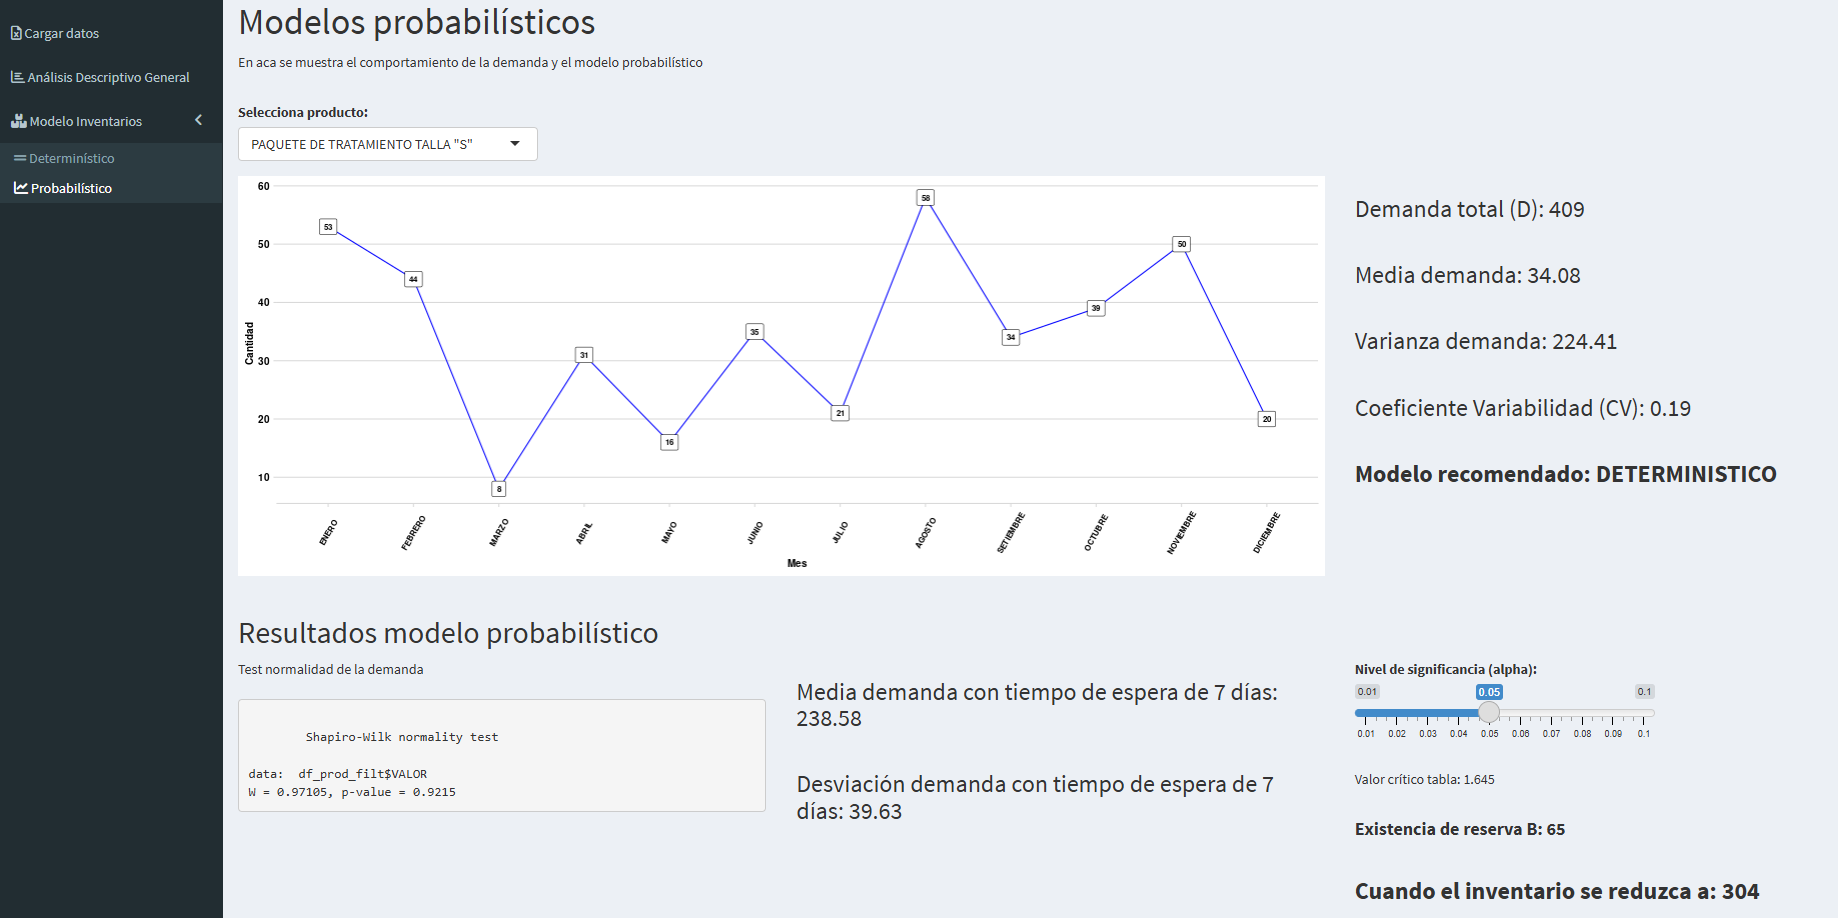
\includegraphics[width=16cm, height=9cm]{images/Shiny8.png}}
  \label{fig:Shiny8}
\end{figure}
\clearpage
La Figura \ref{fig:Shiny8} muestra los resultados obtenidos mediante el modelo probabilizado de la cantidad de pedido, la primera parte muestra los mismos resultados obtenidos en los modelos determinísticos, mientras que en la parte inferior se muestra la siguiente información:

\begin{itemize}
  \item \textbf{Test de normalidad de la demanda:} En esta parte muestra los resultados del test de normalidad usando la prueba de Shapiro-Wilk hacia el comportamiento de la demada, en el cual planteando un nivel de significancia y observado el p-value se decide por aceptar o rechazar la hipótesis nula ($H_0$) acerca de que la demanda mensual se aproxima a una distribución normal.
  \item \textbf{Media demanda con tiempo de espera:} Indica la media de la demanda con respecto al tiempo de entrega.
  \item \textbf{Desviación demanda con tiempo de espera:} Indica la desviación de la demanda con respecto al tiempo de entrega.
  \item \textbf{Nivel de significancia ($\alpha$):} Indica el nivel de significancia que se debe colocar para realizar el cálculo de la cantidad de pedido óptimo.
  \item \textbf{Existencia de reserva ($B$):} Muestra la cantidad de existencia de reserva calculado por el modelo.
  \item \textbf{Nivel de inventario para realizar el pedido:} Indica el momento para realizar el pedido, cuando el inventario llegue a las unidades del modelo se debe de realizar el siguiente pedido.
\end{itemize}




%::::::::::::::::::::::::::::::::::::::::::::::::
%:::::::: PARTE FINAL CONCLUSIONES, RECOMENDACIONES, BIBLIOGRAFIA Y ANEXOS :::::::::::::
%::::::::::::::::::::::::::::::::::::::::::::::::
% Discusiones
\begin{discusiones}
Según el estudio de \cite{gallardo2016propuesta}, titulado \textsl{''Propuesta de mejora para la gestión de inventarios de sociedad repuestos España limitada''} se tuvo un total de 2994 productos estudiados, en los cuales fueron 319 productos clasificados como ``A'' representando el 70$\%$ de las ventas, estos productos fueron analizados de los cuales se tuvieron 102 productos con demanda determinística y 217 productos con demanda probabilística. En la investigación desarrollada se tuvo de un total de 471 productos analizados de los cuales se tuvo 8 productos clasificados como ``A'' representando el $68.55\%$, asimismo se tomaron productos con mayores costos del grupo ``B'' para tener un análisis de 18 productos, en las cuales todos los productos tuvieron una demanda determinística.

La investigación de \cite{loja2015propuesta} titulado \textsl{''Propuesta de un sistema de gestión de inventarios para la empresa FEMARPE CIA.LTDA''} indico que la empresa no lleva fundamentos científicos en las acciones administrativas, sin tener la información necesaria para la aplicación de metodologías propuestas como las 5 S Japonesas, por lo que se recomendó una adecuada organización, estandarización de insumos, autodisciplina del personal, iniciando con la clasificación ABC enfatizando a que productos debe darle la prioridad para evitar gastos adicionales al momento de realizar la aplicación de métodos científicos administrativos. En el estudio realizado en el centro de salud integral La Fuente se observó que se tuvo un gran desarrolló en la parte administrativa, ya que tuvieron un control y registro de todos los movimientos realizados por parte del área de logística, siendo un gran progreso que tuvieron a comparación de los inicios que tuvo la entidad, sin embargo no se tuvo la información exacta en cuanto a la demanda o uso que se daba de cada producto, ya que tuvo que realizarse una estimación en base a los  procedimientos realizados que generalmente usarán los productos, por lo que para este caso se espera que el centro de salud a futuro tenga el registro de estos procesos de productos ya sea usando un software o detallando los registros de salidas por parte del personal que realiza la solicitación.

Por otra parte, al igual que el estudio de \cite{caceres2010propuesta} titulado \textsl{''Propuesta de un modelo de gestión de inventarios que permita mejorar la planeación y la distribución de las medicinas a las farmacias de un hospital''}, es importante tomar en cuenta la composición administrativa y su relación con otras áreas como lo es en el caso de farmacia para poder implantar una mejor política de inventarios, al igual que se tomo la información del KARDEX para ver los movimientos realizados y poder realizar la clasificación por actividades basadas en costos (ABC) en los cuales a pesar de que el centro de salud no tuvo problemas de sobre stock, desabastecimientos y programaciones de abastecimientos al momento de realizar las solicitudes, se espera que la política de inventarios propuesta mejore la gestión de inventarios del centro de salud y asimismo también implantar la metodología para el área de farmacia.

De la misma forma que el estudio de \cite{caballero2007control} titulada \textsl{''Control de inventario para una empresa de capacitación en el área de salud''} se desarrollaron conceptos de sistemas de inventarios para mejorar el desempeño de actividades en la política de inventarios, en el cual el área de logística pueda gestionar eficientemente el sistema de inventarios obteniendo controles óptimos y mejor administración de insumos.

Para este caso no se realizó la aplicación del modelo de inventarios con limitación de almacén como el desarrollado en el trabajo de \cite{koper2017analisis} titulado \textsl{''Análisis del inventario de almacén en la distribuidora Valle Sur S.A. - 2017; mediante el programa de inventario de almacén INVAL''} debido a que a pesar de que los productos tuvieron un área de ocupación en almacén, estos no se ven restringidos obligatoriamente a este espacio, ya que a comparación del estudio en el que se tuvieron que tomar en cuenta los pesos que tuvo cada producto como una limitante al momento de realizar los pedidos, el centro de salud integral no tuvo esos limitantes para los productos, en cambio se recomienda que se vea una mejor opción de almacenamiento especialmente a los productos que tuvieron una clasificación ``A'' mediante las actividades basadas en costos (ABC). Sin embargo a futuro se debería tomar en cuenta estas restricciones de espacio especialmente tomando en cuenta la visión del centro de salud sobre su desarrolló.
	
\end{discusiones}
% Conclusiones
\begin{conclusiones}
	
Según los resultados obtenidos mediante el trabajo de investigación se obtienen las siguientes conclusiones:

\begin{enumerate}
\item Se implementó el modelo clásico de cantidad económica de pedido (EOQ) para optimizar los inventarios de almacén del centro de salud integral La Fuente del Cusco durante el año 2024.
\item Los productos más demandados por el centro de salud integral La Fuente del Cusco en el año 2024 utilizando la metodologías de actividades basadas en costos, son insumos utilizados por el área de oftalmología ocupando el $79.31\%$ de los costos totales de todo el almacén en los que se incluyen los 8 productos clasificados en el grupo A y 10 productos del grupo B, de los cuales las especialidades que tuvieron mayores costos fueron: INLASER ($39.27\%$), FACO ($25.49\%$), insumos generales ($5.97\%$), tintas ($3.78\%$), CROSSLINKING ($2.58\%$), Catarata ($1.52\%$) y esterilización ($0.71\%$). 
\item Los productos seleccionados mediante la metodología (ABC) indicaron un coeficiente de variabilidad menor a 0,20 por lo que se tuvo una demanda determinística y el modelo de inventarios a utilizar en todos los casos era el modelo clásico de cantidad económica de pedido (EOQ).
\item Usando la información brindada por el área de logística y administración del centro de salud integral La Fuente se estableció la cantidad, tiempo y costo óptimo de inventarios asi como el momento de reorden. Pudiendo establecer así la política de inventarios óptima del centro de salud integral.
\item El aplicativo de Shiny apoyará al momento de realizar el monitoreo y seguimiento de los productos, no solo de los productos más demandados, sino también de productos adicionales que se puedan ingresar y pueda apoyar a gestionar una política de inventarios óptima, de la misma forma se incluye el modelo EOQ con escasez y modelo EOQ probabilizado de cantidad pedido.
\item El centro de salud integral La Fuente del Cusco mostró un gran desarrollo con respecto al área administrativa y logística. En el que se espera que la implementación de los modelos de inventarios apoyen en la gestión de las decisiones tomadas acerca de los productos de almacén con base a una administración científica.

\end{enumerate}
	
\end{conclusiones}
 
% Recomendaciones
\begin{recomendaciones}
	
\begin{enumerate}
\item Al centro de salud se recomienda tener el registro sobre el uso de los productos ya sea utilizando algún software o control para tener un valor más preciso al momento de implantar las políticas de inventarios.
\item Evaluar el impacto de la aplicación de modelos de inventarios para la gestión de inventarios con el fin de medir la importancia de la aplicación de modelos de investigación operativa en centros de salud.
\item De la misma forma recomendar la aplicación de sistemas de inventarios en el área de farmacia del centro de salud integral La Fuente para que también se puedan tomar y optimizar los medicamentos gestionados por farmacia.
\item Asimismo se recomienda a las instituciones de diferentes rubros realizar la aplicación de modelos de inventarios y otras técnicas de investigación operativa para llevar una administración científica y mejorar sus procesos. A través de la generación de aplicativos o el uso del aplicativo generado en RShiny.
\item A futuro realizar la aplicación del modelo de cantidad económica de pedido tomando en cuenta la limitación de almacén, asimismo usar los otros tipos de modelos determinísticos y probabilísticos de inventarios a otras problemáticas de aplicación.
\item Asimismo fomentar por parte de la escuela profesional de matemática y estadística al uso de lenguajes de programación como R, especificamente a la generación de aplicativos web con RShiny a los estudiantes para poder realizar prototipos computacionales con las aplicaciones matemáticas, estadísticas y de investigación operativa. De tal forma que puedan aplicar sus ideas de investigación hacia problemas reales de forma práctica e innovadora.
\end{enumerate}
	
\end{recomendaciones}
 

%%%%%%%%%%%%%%%%%%%%%%%%%%%%%%%%%%%%%%%%%%%%%%%%%%%%%%%%%%%%%%%%%%%%%%
\newpage
\bibliographystyle{apalike}
\addcontentsline{toc}{chapter}{BIBLIOGRAFÍA}
\bibliography{contenido/bibliog.bib}
\clearpage
% ANEXOS - Matriz de consistencia
% Capítulos personalizados
\makeatletter
\renewcommand\chapter[1]{%
    \clearpage
    \thispagestyle{empty}
    \phantomsection
    \refstepcounter{chapter}% Actualiza y vincula
    \addcontentsline{toc}{chapter}{#1}%
    \vspace*{\fill}
    \begin{center}
        \normalfont\LARGE\bfseries #1
    \end{center}
    \vspace{\fill}
    \clearpage
    \setcounter{section}{0}
}
\makeatother

% Numeración de secciones en letras
\renewcommand\thesection{\alph{section}.}

% Secciones personalizadas
\makeatletter
\renewcommand\section[1]{%
    \phantomsection
    \refstepcounter{section}%
    \addcontentsline{toc}{section}{\protect\numberline{\thesection}#1}%
    {\normalfont\Large\bfseries \thesection. #1}%
}
\makeatother

\chapter{ANEXOS}

\begin{landscape}
\section{Matriz de consistencia}
%\addcontentsline{toc}{chapter}{ANEXOS}
%\textbf{\Large{ANEXOS}}\\
%\addcontentsline{toc}{section}{A. Matriz de consistencia}
%\textbf{A. Matriz de consistencia}
\begin{table}[h!]
\centering
%\caption{Matriz de Consistencia}
\footnotesize % Reduce el tamaño de la fuente para que quepa mejor
\begin{tabular}{|p{4.5cm}|p{4.5cm}|p{4.5cm}|p{3cm}|p{4.2cm}|}
\hline
\multicolumn{1}{|c|}{\textbf{Problemas}}  & \multicolumn{1}{c|}{\textbf{Objetivos}}  & \multicolumn{1}{c|}{\textbf{Hipótesis}} & \multicolumn{1}{c|}{\textbf{Variables}}   & \multicolumn{1}{c|}{\textbf{Metodología}} \\ \hline
\multicolumn{3}{|c|}{\textbf{General}}                               & \textbf{Dependientes}  & \multirow{4}{=}{
\begin{minipage}{4.2cm}
\justify
$\circ$ \textbf{Tipo:} Aplicado \\
$\circ$ \textbf{Enfoque:} Cuantitativo \\
$\circ$ \textbf{Alcance:} Descriptivo correlacional - Explicativo \\
$\circ$ \textbf{Diseño:} Retrospectivo longitudinal no experimental \\
$\circ$ \textbf{Población:} Productos de almacén. \\
$\circ$ \textbf{Población de estudio:} Productos clasificados mediante (ABC).\\
$\circ$ \textbf{Técnica de recolección de datos:} Revisión documental y/o datos secundarios. \\
$\circ$ \textbf{Instrumento de recolección de datos:} Boletas, ordenes de compra, KARDEX, cotizaciones. \\
$\circ$ \textbf{Método de análisis de datos:} Recopilación de datos en un archivo \textsl{.xlsx}, procesamiento y análisis de datos en el lenguaje de programación R mediante el entorno de desarrollo integrado RStudio.
\end{minipage}
} \\ \cline{1-4}
\multicolumn{1}{|p{4.5cm}|}{¿Cómo implementar los modelos de inventarios para optimizar el control de almacén del centro de salud integral La Fuente del Cusco durante el año 2024?} & \multicolumn{1}{p{4.5cm}|}{Implementar los modelos de inventarios para optimizar el control de almacén del centro de salud integral La Fuente del Cusco durante el año 2024.} & El control de almacén del centro de salud integral La Fuente del Cusco se optimizará mediante la aplicación de los modelos de inventarios. & 
    \vspace{0.2cm}
    $\circ$ Cantidad de pedido óptimo\vspace{0.2cm}

    $\circ$ Tiempo de pedido óptimo\vspace{0.2cm}
  &                       \\ \cline{1-4}
\multicolumn{3}{|c|}{\textbf{Específicos}}                               & \textbf{Independientes} &  \\ \cline{1-4}
\multicolumn{1}{|p{4.5cm}|}{
    $\circ$ ¿Cuáles son los productos más demandados y/o costosos en el centro de salud integral La Fuente del Cusco?\vspace{0.2cm}

    $\circ$ ¿Qué modelo de inventarios se adecua a los productos más demandados y/o costosos del centro de salud integral La Fuente del Cusco?\vspace{0.2cm}

    $\circ$ ¿Cuál es la cantidad, periodo y costos de pedido óptimo para los productos más demandados y/o costosos del centro de salud integral La Fuente del Cusco mediante el modelo de inventarios?\vspace{0.2cm}

    $\circ$ ¿Cómo desarrollar un aplicativo web que apoye con el monitoreo y seguimiento de los productos del centro de salud integral La Fuente del Cusco?} & \multicolumn{1}{p{4.5cm}|}{
    $\circ$ Clasificar los productos más demandados y/o costosos del centro de salud integral La Fuente del Cusco aplicando el análisis de actividades basadas en costo (ABC).\vspace{0.2cm}

    $\circ$ Identificar el mejor modelo de inventarios para los productos más demandados y/o costosos del centro de salud integral La Fuente del Cusco.\vspace{0.2cm}

    $\circ$ Determinar la cantidad, el tiempo y costos de pedido óptimo mediante el modelo de inventarios identificado para los productos más demandados y/o costosos del centro de salud integral La Fuente del Cusco.\vspace{0.2cm}

    $\circ$ Desarrollar un aplicativo web en Shiny para realizar el monitoreo y seguimiento de los productos del centro de salud integral La Fuente del Cusco.

    } & \multicolumn{1}{p{4.5cm}|}{
    $\circ$ Los productos más demandados y/o costosos en el centro de salud integral La Fuente del Cusco vienen a ser aquellos usados en el área de oftalmología.\vspace{0.2cm}

    $\circ$ Los modelos de inventarios determinísticos se adecuan a los productos más demandados y/o costosos.\vspace{0.2cm}

    $\circ$ Las cantidades, tiempo y costos de inventarios se optimizarán aplicando los modelos de inventarios.\vspace{0.2cm}

    $\circ$ El aplicativo web de Shiny monitoreara y dara seguimiento a los productos del centro de salud integral La Fuente del Cusco.

    } & \multicolumn{1}{p{3cm}|}{
    \vspace{0.2cm}
    $\circ$ Tiempo de reabastecimiento.\vspace{0.2cm}

    $\circ$ Demanda.\vspace{0.2cm}

    $\circ$ Costos.
    }  & \\ \hline
\end{tabular}
\end{table}


 
% Matriz de consistencia
%\begin{matriz_consistencia}

\begin{landscape}
\textbf{\Large{ANEXO}}%\\
%\textbf{\normalsize{Matriz de consistencia}}\\
\begin{table}[h!]
\centering
\caption{\textbf{\textsl{Matriz de Consistencia}}}
\footnotesize % Reduce el tamaño de la fuente para que quepa mejor
\begin{tabular}{|p{4.2cm}|p{4.2cm}|p{4.2cm}|p{4.2cm}|p{4.2cm}|}
\hline
\multicolumn{1}{|c|}{\textbf{Problemas}}  & \multicolumn{1}{c|}{\textbf{Objetivos}}  & \multicolumn{1}{c|}{\textbf{Hipótesis}} & \multicolumn{1}{c|}{\textbf{Variables}}   & \multicolumn{1}{c|}{\textbf{Metodología}} \\ \hline
\multicolumn{3}{|c|}{\textbf{General}}                               & \textbf{Dependientes}  & \multirow{4}{=}{
\begin{minipage}{4.2cm}
\justify
$\circ$ \textbf{Tipo:} Aplicado \\
$\circ$ \textbf{Nivel:} Descriptivo Correlacional - Explicativo \\
$\circ$ \textbf{Diseño:} Retrospectivo longitudinal no experimental \\
$\circ$ \textbf{Población:} Todos los productos de almacén. \\
$\circ$ \textbf{Población de estudio:} Productos clasificados en el grupo A mediante (ABC).\\
$\circ$ \textbf{Técnica de recolección de datos:} Revisión documental y/o datos secundarios. \\
$\circ$ \textbf{Instrumento de recolección de datos:} Boletas, ordenes de compra, KARDEX, cotizaciones. \\
$\circ$ \textbf{Método de análisis de datos:} Recopilación de datos en un archivo \textsl{.xlsx}, procesamiento y análisis de datos en el lenguaje de programación R mediante el entorno de desarrollo integrado RStudio.
\end{minipage}
} \\ \cline{1-4}
\multicolumn{1}{|p{4.2cm}|}{¿Cómo es la gestión de inventarios de almacén sobre los productos más demandados del centro de salud integral La Fuente?} & \multicolumn{1}{p{4.2cm}|}{Analizar la gestión de inventarios del almacén en el centro de salud integral La Fuente mediante los modelos de inventarios.} & La gestión de inventarios de almacén sobre los productos más demandados del centro de salud integral ``La Fuente'' es óptimo. & 
    \vspace{0.2cm}
    $\circ$ ¿Cuánto pedir?\vspace{0.2cm}

    $\circ$ ¿Cuándo pedir?\vspace{0.2cm}
  &                       \\ \cline{1-4}
\multicolumn{3}{|c|}{\textbf{Específicos}}                               & \textbf{Independientes} &  \\ \cline{1-4}
\multicolumn{1}{|p{4.2cm}|}{
    $\circ$ ¿Cuáles son los productos más demandados y/o utilizados en el centro de salud integral La Fuente?\vspace{0.2cm}

    $\circ$ ¿Que modelo de inventarios se adecua a los productos más demandados?\vspace{0.2cm}

    $\circ$ ¿Cuál es la cantidad, periodo y costos de pedido óptima para los productos de productos más demandados del centro de salud integral La Fuente mediante el modelo de inventarios?\vspace{0.2cm}

    $\circ$ ¿Cómo desarrollar un seguimiento a los productos más demandados?} & \multicolumn{1}{p{4.2cm}|}{
    $\circ$ Clasificar los productos más demandados del centro de salud integral La Fuente aplicando el análisis de actividades basadas en costo (ABC).\vspace{0.2cm}

    $\circ$ Seleccionar el mejor modelo de inventarios de los productos más demandados.\vspace{0.2cm}

    $\circ$ Determinar mediante el modelo de inventarios la cantidad, el tiempo y costos de pedido óptimo para los productos más demandados del centro de salud integral La Fuente.\vspace{0.2cm}

    $\circ$ Desarrollar un app web en Shiny para realizar el monitoreo y seguimiento de los productos más demandados del centro de salud integral La Fuente.

    } & \multicolumn{1}{p{4.2cm}|}{
    $\circ$ Los productos más demandados y utilizados en el centro de salud integral ``La Fuente'' vienen a ser aquellos usados en el área de oftalmología.\vspace{0.2cm}

    $\circ$ Los modelos de inventarios determinísticos se adecuan a los productos más demandados..\vspace{0.2cm}

    $\circ$ Las cantidades, tiempo y costos de pedidos se optimizarán aplicando modelos de inventarios determinísticos.\vspace{0.2cm}

    $\circ$ Los seguimientos se desarrollarán en función a la demanda en el tiempo para realizar la adquisición de inventarios nuevas que van ingresar al almacén tomando en cuenta el modelo de inventario más óptimo del producto.

    } & \multicolumn{1}{p{4.2cm}|}{
    \vspace{0.2cm}
    $\circ$ Tiempo de reabastecimiento.\vspace{0.2cm}

    $\circ$ Demanda.\vspace{0.2cm}

    $\circ$ Costos.
    }  & \\ \hline
\end{tabular}
\end{table}

\end{landscape}
\end{matriz_consistencia}

\end{document}
